\documentclass{article}
\usepackage{enumitem}
\usepackage{layout}
\usepackage[utf8]{inputenc}
\usepackage{graphicx}
\usepackage[T2A]{fontenc}
\usepackage[bulgarian]{babel}
\usepackage{amssymb}
\usepackage{amsthm}  % For theorem environments
\usepackage{mathtools}
\usepackage{algpseudocode}
\usepackage{algorithm}
\usepackage{parskip}
\usepackage{stmaryrd}
\usepackage{marvosym}
\usepackage{tikz}
\usepackage{listings}
\usetikzlibrary{trees}
\usepackage[a4paper,margin=0.7in]{geometry}  % Adjust margin size
\usepackage{cancel}
\graphicspath{ {images/}}
\renewcommand{\\}{\newline}
\renewcommand{\labelenumii}{\arabic{enumi}.\arabic{enumii}}
\algrenewcommand{\alglinenumber}[1]{@\footnotesize#1.} % algorithm customization
\newcommand{\Dashv}{\rotatebox[origin=c]{180}{$\vDash$}}
\newcommand{\symvDash}{\mathrel{\vDash\!\!\!\!\!\Dashv}}
\let\marvosymLightning\Lightning
\newcommand{\amp}{\;\&\;}
\newcommand{\sep}{\;|\;}
\newcommand{\df}[1]{\textbf{Дефиниция:} \underline{#1}:\\}
\newcommand{\tv}{\textbf{Твърдение:\;}}
\newcommand{\tm}{\textbf{Теорема:\;}}
\newcommand{\mc}{\mathcal}
\newcommand{\N}{\mathbb{N}}
\newcommand{\R}{\mathbb{R}}
\newcommand{\spc}{\\\hfill \break}
\newcommand{\arrowdef}{ \overset{\text{def}}{\iff}}
\newcommand{\zad}[1]{\textbf{Задача #1:}}
\newcommand{\eqs}[1]{\begin{equation*}\begin{aligned} #1 \end{aligned}\end{equation*}}
\newcommand{\linia}{\spc\rule{\textwidth}{0.3pt}\vspace{2ex}\\}
\newcommand{\doc}{\textbf{Доказателство: }}
\newcommand{\ii}{\text{ и }}
\newcommand{\I}{\text{И}}
\newcommand{\lu}{\text{Л}}
\newcommand{\proven}{\hfill $\square$}
\DeclarePairedDelimiter{\set}{\{}{\}}
\lstset{
    language=SQL,
    basicstyle=\small\ttfamily,
    keywordstyle=\color{blue}\bfseries,
    commentstyle=\color{gray},
    stringstyle=\color{purple},
    breaklines=true,
    frame=single,
    showstringspaces=false
}
\begin{document}
\title{Подготовка за държавен изпит}
\author{Алекс Трифонов}
\date{}
\maketitle{}
\section{Множества. Декартово произведение. Релации. Функции.}
  \subsection{Аксиоматизация на множествата: аксиоми за обема, отделянето, степенното множество и индиктивно генерираните множества. }
    \textit{Аксиома за обема}: Ако две множества имат едни и същи елементи, то те са равни. 
    \[
      \forall x \forall y \left( \forall z \left( z \in x \iff z \in y \right) \Rightarrow x = y \right)
    \] 

    \textit{Схема за отделянето}: Нека \(\varphi(x, u_1, \dots, u_n\) е теоретикомножествено свойство. Тогава за всяко множество \(A\) съществува множество \(B\), чиито елементи са точно онези елементи от \(A\), които имат свойство \(\varphi\). 

    \[
      \forall u_1\dots\forall u_n \forall A \exists B \forall x \left[ x \in B \iff (x \in A \& \varphi(x, u_1, \dots, u_n)) \right]
    \]   

    \textit{Аксиома за степенното множество}: За всяко множество \(A\) съществува множество \(B\), измежду чиито елементи за всички подмножества на \(A\). 
    \[
      \forall A \exists B \forall x \left( x \subseteq A \Rightarrow x \in B \right)
    \] 

    \textit{Аксиома за индуктивно генерираните множества}: Нека \(M_0\) е непразно множество, а \(F\) е множество от операции. Тогава \(M\) се ствои по следния начин:
    \begin{enumerate}[label = \arabic*., leftmargin=*]
        \item База: \(M_0 \subseteq M\) 
        \item Индукционно предположение: Нека \(M \not= \emptyset\)
        \item Индукционна стъпка: \(M_i  = M_{i-1} \cup \left\{ f(m_i)  \sep f \in  F \& m_{i-1} \in M_{i-1}  \right\}\)   
        \item Заключение: В \(M\) няма други елементи освен базовите и включенито от индукционна стъпка, т.е. \(M = \left\langle M_{0}, F \right\rangle\)   
    \end{enumerate}

\subsection{Математичекса индукция.}

    \textit{Принцип на слабата математическа индукция}: Нека \(m, n \in \mathbb{N}, n \geq m\). За всяко свойство \(\varphi(n)\), ако \(\varphi(m)\) е истина и \(\left( \forall k > m \right)(\varphi(k) \Rightarrow \varphi(k+1))\), то \(\forall n \in \mathbb{N} (\varphi(n))\)     

    \textit{Принцип на силната математическа индукция}: Нека \(m, n \in \mathbb{N}, n \geq m\). За всяко свойство \(\varphi(n)\), ако \(\varphi(m)\) е истина и \(\left( \forall k > m \right)(\underset{i = m}{\overset{k-1}{\land}} \varphi(i) \Rightarrow \varphi(k))\), то \(\forall n \in \mathbb{N} (\varphi(n))\)     

\subsection{Основни операции върху множества и техните свойства }
\textit{Операции}: Нека \(A, B\) са множества.
       \begin{itemize}
       \item Обединение: \(A \cup B = \left\{ x \sep x \in B \lor x \in A \right\}\)  
       \item Сечение: \(A \cap B = \left\{ x \sep x \in B \land x \in A \right\}\)  
       \item Допълнение: \(\bar{A} = \left\{ x \sep x \not\in A \right\} \)
       \item Разлика: \(A \setminus B = \left\{ x \sep x\in A \land x \not\in B\right\} \)
       \item Симетрична разлика: \(A \delta B = (A \setminus B) \cup (B\setminus A)\)
       \item Степенно множество: \(\mathcal{P}(A) = \left\{ x \sep x \subseteq A \right\}\)  
       \item Обединение на \(\left\{A_1,...,A_n\right\}\): \(\underset{i=1}{\overset{n}{\bigcup}}A_i=\left\{x \sep \exists i (1 \leq i \leq n \& x \in A_i) \right\} \)
       \item Сечение на \(\left\{A_1,...,A_n\right\}\): \(\underset{i=1}{\overset{n}{\bigcap}}A_i=\left\{x \sep \forall i (1 \leq i \leq n \& x \rightarrow A_i) \right\}\)
        
       \end{itemize}

    \textit{Свойства} Нека \(A, B, C\) са множества. 
      \begin{itemize}
          \item Идемпотентност: \(A \cup A = A, A \cap A = A\)  
          \item Комутативност: \(A \sigma B = B \sigma A,\; \sigma \in \left\{\cup, \cap, \delta \right\}\)  
          \item Асоциативност: \((A \sigma B) \sigma C = A \sigma (B \sigma C),\; \sigma \in \left\{\cup, \cap, \delta \right\}\)  
          \item Свойства на универсума: \(\Omega \cup A = \Omega, \Omega \cap A = A\)
          \item Свойства на празното множество: \(\emptyset \cup A = A, \emptyset \cap A = \emptyset\)  
          \item Свойства на допълнението: \(A \cup \bar{A} = \Omega, A \cap \bar{A} = \emptyset\)  
          \item Закон на Де Морган: \(\bar{A \cup B} = \bar{A} \cap \bar{B}, \bar{A \cap B} = \bar{A} \cup \bar{B}\)  
      \end{itemize}

      \subsection{Наредена двойка и наредена n-орка }
    \textit{Наредена двойка}: За два елемента \(a, b\) въвеждаме операцията наредена двойка \(\left\langle a, b \right\rangle\). Наредената двойка \(\left\langle a, b \right\rangle\) има следното свойство: 
    \[
      a_{1}=a_{2}\land b_{1}=b_{2} \iff \left\langle a_1, b_1 \right\rangle = \left\langle a_2, b_2 \right\rangle
    \] 

    \textit{Наредена двойка на Куратовски}: \(\left\langle a, b \right\rangle = \left\{\left\{ a \right\}, \left\{ a, b \right\} \right\}\)  

    \textit{Наредена n-торка}: Нека \(a_1, \dots, a_n, n\geq2\) са произволни елементи. Наредена n-орка на елементите \(a_1,\dots, a_n\) наричаме \(\left\langle a_1,\dots, a_n \right\rangle = \left\langle a_1, \left\langle a_2, \left\langle ..., a_n \right\rangle \right\rangle \right\rangle\)    
    
    \subsection{Декартово произведение и обобщено Декартово произведение. }
    \textit{Декартово произведение}: За две множества \(A, B\) определяме тяхното декартово произведение като: \[
      A \times B = \left\{ \left\langle a, b \right\rangle \sep a \in A \& b \in B \right\}
    \]    

    \textit{Обобщено Декартово произведение}: За краен брой множества \(A_1, \dots, A_n\) определяме: \[
    A_1 \times ... \times A_n = \left\{\left\langle a_1, \dots, a_n \right\rangle \sep a_1 \in A_1, \dots, a_n \in A_n \right\}
    \]  

    \subsection{Релация над n домейна }
    \textit{Релация над n домейна}: Нека \(A_1,\dots,A_n\) са множества. Всяко подмножество \(R\) на Декартовото произведение на \(A_1,\dots,A_n\) наричаме n-местна релация над \(A_1,\dots,A_n\). За \(n=2\) казваме, че \(R\) е бинарна релация. 

    \textit{Domain, range}
      \[
        Dom(R)=\left\{a\sep a \in A \& (\exists b \in B)[\left\langle a, b\right\rangle \in R]\right\}
      \]
      \[
        Range(R)=\left\{b\sep b \in B \& (\exists a \in A)[\left\langle a, b\right\rangle \in R]\right\}
      \]      

      \subsection{Свойства на бинарните релации }
    Нека \(R \subseteq A \times A\). 
    \begin{itemize}
      \item \(R\) е рефлексивна  \(\iff \left(\forall x \in A\right)[\left\langle x, x\right\rangle \in R]\)   
      \item \(R\) е транзитивна  \(\iff \left(\forall x, y, z \in A\right)[\left\langle x, y\right\rangle \in R \& \left\langle y, z\right\rangle \in R \Rightarrow \left\langle x, z\right\rangle \in R]\)   
      \item \(R\) е симетрична  \(\iff \left(\forall x, y \in A\right)[\left\langle x, y\right\rangle \in R \Rightarrow \left\langle y, x\right\rangle \in R]\)   
      \item \(R\) е антисиметрична  \(\iff \left(\forall x, y \in A\right)[\left\langle x, y\right\rangle \in R \& \left\langle y, x\right\rangle \in R \Rightarrow x = y]\)   
      \item \(R\) е силно антисиметрична  \(\iff \left(\forall x, y \in A\right)[\left\langle x, y\right\rangle \in R \Rightarrow \left\langle y, x\right\rangle \not\in R]\)   
    \end{itemize}

    \subsection{Релация на еквивалентност и класове на еквивалентност }
    \textit{Релация на еквивалентност}: Нека \(A \not=\emptyset\) е множество. Релация \(R\) над \(A\) наричаме релация на еквивалентност ако \(R\) е симетрична, рефлексивна и транзитивна.    

    \textit{Клас на еквивалентност}: Нека \(A\) е множество, \(a \in A\) и \(R\) е релация на еквивалентност над \(A\). Класът на еквивалентност на \(a\) по отношение на релацията \(R\) е множеството: \[
      [a]_{R} = \left\{b \in A \sep \left\langle a, b\right\rangle\in R\right\}
    \]        

    Всяка релация на еквивалентност на множеството поражда разбиване на множеството.
  

    \subsection{Релации на частична наредба }
    \textit{Релация на частична наредба}: Релацията \(R\) над \(A\) е релация на частична наредба, ако \(R\) е рефлексивна, антисиметрична и транзитивна.    

    \textit{Релация на строга частична наредба}: Релацията \(R\) над \(A\) е релация на строга частична наредба, ако \(R\) е антирефлексивна, антисиметрична и транзитивна.    

    \subsection{Диаграми на Хассе }
    \textit{Диаграми на Хассе}: графично представяне на бинарна релация \(R \subseteq A \times A\), където всеки елемент на \(A\) се изобразява като връх и за всеки елемент \(\left\langle a, b\right\rangle \in R\) поставяме стрелка от \(a\) към \(b\).      

    \subsection{Релации на пълна наредба }
    \textit{Пълна наредба}: Нека \(A\) е множесто и \(R\) е релация над \(A\). \(R\) е пълна наредба над \(A\), ако \(R\) е (строга) частична наредба и всеки два различни елемента от \(A\) са сравними по отношение на \(R\). 
    \[
      \forall a \in A \forall b \in A (a \not=b \rightarrow (\left\langle a,b \right\rangle \in R \lor \left\langle b, a\right\rangle \in R))
    \] 

    Пример за пълна наредба са релациите \(\leq, <\) над естествените числа.  

    \subsection{Минимален и максимален елемент в релация на частична наредба }
    Нека \(R\) е частична наредба над множеството \(A\). Казваме, че \(a \in A\) e:
    \begin{itemize}
        \item Минимален елемент по отношение на \(R\), ако \(\forall b \in A (a \not= b \Rightarrow \left\langle b, a\right\rangle \not \in R\)   
        \item Максимален елемент по отношение на \(R\), ако \(\forall b \in A (a \not= b \Rightarrow \left\langle a, b \right\rangle \not \in R\)   
    \end{itemize}

    \subsection{Влагане на частична наредба в пълна наредба - топологично сортиране }
    \textbf{Теорема}: Нека \(A \not=\emptyset\) е крайно множество и \(R\) е частична наредба над \(A\). Тогава съществува пълна наредба \(S\) над \(A\), т. че \(R \subseteq S\)
     
    \doc Нека за определеност \(R\) е нестрога частична наредба.   

    Нека \(\left|A\right| = n\) (крайно, непразно). Ще докажем, че елементите на \(A\) могат да се подредят в редица. Тъй като \(A\) е крайно множество, то \(A\) има минимален и максимален елемент по отношение на \(R\). 
    \begin{itemize}
        \item База: Нека \(a_1\) е един такъв минимален елемент на \(A\) 
        \item И.Х. Нека сме построили редицата \(a_1,\dots, a_{i}\) от i на брой различни елемента на \(A\) 
        \item И.С. Ако \(i=1\), край на конструкцията и \(A = \left\{a_1,\dots, а_n\right\}\)   

          Иначе \(A_{i} = A \setminus \left\{a_1,\dots,a_i\right\}\) е непразно, а \(R \cap (A_i \times A_i)\) е частична наредба над \(A_i\). Избираме минимален елемент \(a_{i+1}\) на \(A_i\) по отношение на \(R \cap A_i \times A_i\)      
    \end{itemize}

    След като сме подредили елементите на \(A\) като \(a_1,\dots,a_n\) дефинираме релацията \(S = \left\{\left\langle a_i, a_j\right\rangle\sep 1 \leq i \leq j \leq n\right\}\). Твърдим, че \(S\) е пълна наредба над \(A\)\dots

    \begin{itemize}
        \item Всеки елемент на \(A\) присъства в редицата, т.е. \(a = a_i\). Имаме, че \(i \leq i, \left\langle a_i, a_i\right\rangle \in S\), откъдето \(S\) е рефлексивна.   
        \item Антисиметричността и транзитивността на \(S\) следват от антисиметричността и транзитивността на \(\leq\) над \(\mathbb{N}\) ???    
        \item Нека \(a, b \in A\), тогава за някои \(i, j\) имаме, че \(a = a_i, b = b_j\). Ако \(i \leq j\) то \(\left\langle a, b\right\rangle\in S\) , иначе \(\left\langle b, a\right\rangle\in S\)      
    \end{itemize}

    Оттук \(S\) е пълна наредба.

    Проверка, че \(R \subseteq S\). Нека \(\left\langle a, b\right\rangle\in R\). Тогава имаме, че \(a = a_i, b = a_j\) за някои \(i, j\). Да допуснем, че \(j < i\), т.е. \(\left\langle b, a\right\rangle \in R\). Имаме, че на стъпка \(j\) в конструирането на редицата елементът \(b\) е минимален на \(A_j\) спрямо \(R \cap (A_i\times A_i)\) и не се среща в \(a_1,\dots,a_{j-1}\). По същият начин \(a = a_i\) не се среща в \(a_1,\dots,a_{j-1}\), защото \(j < i\), откъдето \(a_i \in A_j\setminus \left\{a_1,\dots,a_{j-1}\right\}\). 
    Така \(\left\langle a, b\right\rangle \in R \cap (A_i \times A_i)\), но това противоречи с минималността на \(R\). Следователно \(i \leq j\) и \(\left\langle a, b\right\rangle \in S\)     

    \subsection{Частични и тотални функции }
    \textit{Частична функция}: Релацията \(R \subseteq A \times B\) се нарича тотална функция от \(A\) в \(B\), ако \(\forall a \in A \exists\) поне едно \(b \in B\), т. че \(\left\langle a, b\right\rangle \in R\)    

    \textit{Тотална функция}: Релацията \(R \subseteq A \times B\) се нарича тотална функция от \(A\) в \(B\), ако:
      \begin{itemize}
          \item \(\forall a \in A \exists b \in B \left\langle a, b\right\rangle \in R\) 
          \item \(\forall a \in \forall b_1, b_2 \in B [(\left\langle a, b_1\right\rangle \in R \land \left\langle a, b_2\right\rangle \in R \rightarrow b_1 = b_2\)  
      \end{itemize}

    Означаваме функциите като \(f: A \to B\) и пишем \(f(a) = b\) вместо \(\left\langle a, b\right\rangle \in f\)    

    \subsection{Инекции, биекции и сюрекци }
    Казваме, че функцията \(f: A \to B\) e:
    \begin{itemize}
        \item Инекция (еднозначна), ако \(\forall a_1, a_2 \in A [a_1 \not= a_2 \rightarrow f(a_1) \not= f(a_2)\)  
        \item Сюрекция, ако \(\forall b \in B \exists a \in A f(a) = b\)  
        \item Биекция, ако е инекция и сюрекция.
    \end{itemize}

    \subsection{Дефиниция на крайно множество и на кардиналност на крайно множество }
    \textit{Крайно множество}: Множеството \(A\) е крайно ако \(A = \emptyset\) или \(\exists n \in \mathbb{N}\setminus \left\{0\right\}\), т. че  има биекция между \(A\) и \(I_{n} = \left\{0,\dots, n-1\right\}\)

    \textit{Кардиналност}: Броят на елементите на множеството \(A\). Бележим с \(\left|A\right|\)    

    \subsection{item Дефиниция на изброимо безкрайно множество }
   \textit{Изброимо безкрайно множество}: Нека \(A\) е множество. Казваме, че \(A\) е изброимо безкрайно множество, ако има биекция между \(A\) и \(\mathbb{N}\)   

   \subsection{Приницип на Дирихле }    Нека \(X\) е множество от \(n\) елемента (предмета), \(Y\) е множество от \(m\) елемента (чекмеджета) и \(n > m\). Тогава за всяка тотална функция \(f: X \to Y \exists a \not= b \in X\), т.че \(f(a) = f(b)\)        

\newpage
\section{Основни комбинаторни принципи и конфигурации. Рекурентни уравнения.}
  \subsection{Формулировки на принципите на изброителната комбинаторика - принцип на Дирихле, събирането, изваждането, умножението, делението, включване и изключване. }

      \textit{Принцип на Дирихле}: Нека \(X, Y\) са крайни множества като \(\left|X\right| > \left|Y\right|\). Тогава за всяка тотална функция \(f: X \to Y\) съществува \(a \not= b \in X:\; f(a) = f(b)\)     

      \textit{Прнцип на биекцията}: Нека \(A, B\) са крайни множества. \(\left|A\right| = \left|B\right|\) т.с.т.к. съществува биекция \(f: A \to B\)    

      \textit{Принцип на събирането}: Нека \(A\) е крайно множество, а \(P = \left\{S_1, \dots, S_k\right\}\) е разбиване на \(A\). Тогава \(\left|A\right|=\underset{i=1}{\overset{k}{\left|S_i\right|}}\) 
      \textit{Принцип на изваждането}: Нека \(A\) е множество в универсум \(\Omega\). Тогава \(\left|A\right| = \left|\Omega\right|-\left|\bar{A}\right|\)

      \textit{Принцип на умножението}: Нека \(A, B\) са крайни множества и \(\left|A\right|=n, \left|B\right|=m\). Тогава \(\left|A \times B\right| = \left|A\right|.\left|B\right|=n.m\)    

      \textit{Принцип на делението}: Нека \(A\) е множество. Нека \(R \subseteq A^{2}\) е релация на еквивалентност. Нека \(A\) има \(k\) класа на еквивалентност и всеки клас има кардиналност \(m\). Тогава \(m =\frac{\left|A\right|}{k}\) 

      \textit{Принцип на включването и изключването}: Нека \(A_1, \dots, A_n\) са множества. Тогава:
      \[
        \left|A_1\cup\dots\cup A_n\right|=\sum_{i=1}^{n}\left|A_i\right| - \sum_{1 \leq i \leq j \leq n}\left|A_i \cap A_j\right| + \dots + (-1)^{n-1}\left|A_1 \cap \dots \cap A_n\right|
      \] 

      \doc Индукция по \(n\). 
      \begin{itemize}
          \item База: При \(n=1\) имаме \(\left|A_1\right|=\left|A_1\right|\)   
          \item И.Х.: Нека е вярно за \(n-1\) 
          \item И.С.: Имаме, че \(\left|A_1 \cup \dots A_{n-1} \cup A_{n}\right| = \left|A_1 \cup \dots A_{n-1}\right| +  \left|A_n\right| - \left|(A_1 \cup \dots A_{n-1}) \cap A_n\right|\)  

            От И.Х. знаем колко е \(\left|A_1 \cup \dots A_{n-1}\right|\). Разглеждаме \((A_{1} \cup A_{n-1}) \cap A_{n} = (A_{1} \cap A_n) \cup \dots (A_{n-1} \cap A_{n})\). 

            Но това е обединение на \(n-1\) множества следователно можем да приложим И.Х. Получаваме:
            \[
              \left|(A_{1} \cup \dots A_{n-1}) \cap A_{n}\right| = \sum_{i=1}^{n-1}\left|A_{i} \cap A_{n}\right| - \sum_{1 \leq i \leq j}\left|A_{i} \cap A_{n} \cap A_{j}\right|- \dots + (-1)^{n-1-1}\left|A_1 \cap \dots A_{n-1} \cap A_{n}\right|
            \] 

            Обединявайки с горното имаме:
            \begin{align*}
              & -\sum_{1 \leq i \leq j \leq n - 1}(\left|A_{i} \cap A_{j}\right|) - \sum_{1 \leq i \leq n-1}(\left|A_{i}\cap A_{n}\right|) = \sum_{1 \leq i \leq j \leq n}(\left|A_{i} \cap A_{j}\right|) \\
              & \vdots \\
            \end{align*}

            И получаваме търсеното.
      \end{itemize}

      \subsection{Основните комбинаторни конфигурации: с или без наредба, с или без повтаряне. Извеждане на формулите за броя на основните комбинаторни конфигурации.} 
      Дадени са ни \(n\) обекта и искаме да изберем \(k\) от тях. Изаборът е функция \(f: \left\{1,\dots,k\right\}\to \left\{1,\dots,n\right\}\). По колко начина можем да направим този избор, т.е. колко са функциите \(f\)?

      \textit{Конфигурация с повторение, с наредба}: Нека \(A\) и \(B\) са множества, т.че \(\left|A\right|=k, \left|B\right|=n\). Тогава броят на функциите \(f: A \to B\) е \(n^{k}\). 

      \textbf{Доказателство}: Индуцкия по \(k\):
      \begin{itemize}
          \item \(k=0\): Тогава \(A=\emptyset\) и има единствена функция \(f=\emptyset: A \to B\) 
          \item \(k \geq 1\) и нека \(A=\left\{a_{1}, \dots, a_{k}\right\}\). Всяка функция \(f: A \to B\) можем да представим едниозначно чрез вектора на нейните стойности: \[ f = \left(f(a_{1},\dots, f(a_{n})\right) \in B^{k} \]

        Съгласно принципа на биекцията, броят на различните функции е същият като броя на елементите на \(B^{k}\). Съгласно прниципа на умножението \(\left|B^{k}\right| = n^{k}\)   
        
      \end{itemize}

      \textit{Конфигурация с наредба, без повторениe}: Тъй не може да имаме повтаряне на обекти, функцията трябва да е инекция. Броят на инекциитe \(f: A \to B\) е \(n(n-1)\dots(n-k+1) = \prod_{i=0}^{k-1}(n-i)\)    

      \doc \begin{itemize}
          \item Ако \(k > n\), то от принципа на Дирихле няма инекция \(f: A \to B\). Формулата оставя вярна, защото един от множителите ще е 0. 
          \item Ако \(k=0\), то \(A=\emptyset\) и функцията \(f=\emptyset: A \to B\) е инекция. 
          \item Нека \(1 \leq k \leq n\). Нека \(A = \left\{a_{1},\dots,a_n\right\}\). Всяка инекция \(f: A \to B\) можем да представим еднозначно чрез вектора от нейните стойности: \(f=\left(f(a_{1}) \dots f(a_{k})\right)\in B^{k}\). Имаме, че \(a_{1},\dots, a_{k}\) са различни и съгласно принципа за умножението получаваме \(\prod_{i=0}^{k-1}(n-i)\) възможностти.      
      \end{itemize}

      \textit{Конфигурации без повторение, без наредба}: Броят на \(k\)-елемнтните подмножества на множество с \(n\) елемента е \(\binom{n}{k}\)

      \doc Ако \(k \geq n\), няма \(k\)-елементни помножества на множество с \(n\)   елемента и формулата е вярна. 

      Нека \(k \leq n\) и \(A\) е множество. Индукция по \(n \):
      \begin{itemize}
        \item \(n = 0, A = \emptyset\). Единствената възможност за \(k\) е \(k = 1 = \frac{n!}{0!(n-0!)} = \binom{n}{0}\), защото единственото подмножество на празното е празното. 
        \item Нека е вярно за всяко \(k \leq n\) 
        \item Нека \(A = \left\{a_{1},\dots, a_{n+1}\right\}\) и \(k \leq n + 1\)  

          \begin{itemize}
              \item \(k = 0\) получаваме празното множество, което е единственото подмножество на \(А\) с 0 елемента.   
              \item Ако \(k = n + 1\) то единственото подмножество на \(A\) с \(n+1\) елемента е самото \(A\). Имаме: \(1 = \binom{n+1}{n+1}\)      
              \item \(1 \leq k \leq n\). Разделяме \(k\)-елементните подмножества на две непрсичащи се групи: тези, които съдържат \(a_{n+1}\) и тези, които не съдържат \(a_{n+1}\).
                Съгласно И.Х. тези от втората група са \(\binom{n}{k}\) на брой. 

                Елементите от първата група са от вида \(\left\{a_{n+1}\cup X\right\}\), където \(X\) е някое \(n-1\) елементно подмножество на \(\left\{a_{1},\dots,a_{n}\right\}\). Броят на елементите от тази група са колкото на \(X\), което от И.Х ни дава \(\binom{n}{k-1}\) на брой. 

                Събирайки двете получаваме: \[
                  \binom{n}{k} + \binom{n}{k-1} = \frac{n!}{k!(n-k)!} + \frac{n!}{(k-1)!(n-k-1)!} = \frac{n!}{(k-1)!(n-k)!(\frac{1}{k} + \frac{1}{n-k+1})} = \frac{(n+1)!}{k!(n+1-k)!} = \binom{n+1}{k}
                \]
          \end{itemize}

      \end{itemize}

                \textit{Конфигурация без наредба, с повторение}: Трябва да изберем \(k\) предмета измежду \(n\) вида, като наредбата няма значение. От принципа на биекцията задачата се свежда до начините, по които можем да изберем \(k-1\) кутии, в които да поставим \(n\) обекта. Общо \(\binom{n+k-1}{k-1}\)   


                \subsection{Биномни коефициенти и теорема на Нютон.}
      \textit{Теорема на Нютон}: Нека \(x, y \in \mathbb{R}, n \in \mathbb{N}\). Тогава: \[
        (x+y)^{n} = \sum_{k=0}^{n}\binom{n}{k}x^{k}y^{n-k}
      \] 

      \doc Индукция по \(n\):

      \begin{itemize}
        \item \(n=0: (x+y)^{0} = 1 = \binom{0}{0}x^{0}y^{0-0}\)  
        \item Нека твърдението е в сила за \(n\) 
        \item \begin{align*}
            (x+y)^{n+1} &= (x+y)^{n}(x+y) = \left(\sum_{k=0}^{n}\binom{n}{k}x^{k}y^{n-k}\right)(x+y) = \\
                        &= \sum_{k=0}^{n}\binom{n}{k}x^{k+1}y^{n-k} + \sum_{k=0}^{n}x^{k}y^{n-k+1} = \\
                        &= \binom{n}{0}xy^{n} + \binom{n}{1}x^{2}y^{n-1}\dots + \binom{n}{n}x^{n+1} + \\
                        &+ \binom{n}{0}y^{n+1} + \binom{n}{1}xy^{n}\dots + \binom{n}{n}x^{n}y + \\
                        &= \binom{n+1}{0}y^{n+1} + \left(\binom{n}{0} + \binom{n}{1}\right)xy^{n} + \dots + \binom{n+1}{n+1}x^{n+1} =\\
                        &= \sum_{k=0}^{n+1}\binom{n+1}{k}x^{k}y^{n+1-k}
        \end{align*}
      \end{itemize}
    
     \subsection{Доказателства на комбинаторни тъждества чрез комбинаторни разсъждения.}
      \textit{Свойство}: \[
        \binom{n}{k} = \binom{n-1}{k} + \binom{n-1}{k-1}
      \] 


      \textit{Свойство}: \[
        \binom{n}{m} = \binom{n}{n-m}
      \] 

      \subsection{Алгоритъм за решаване на линейни рекурентни уравнения с константни коефициенти - хомогенни и нехомогенни.} 
      \textit{Рекурентно отношение от ред \(r\)}: Нека \(a_0, \dots, a_{r-1}\) са членове на редицата \(a_{n} = f(a_{n-1}, \dots, a_{n-r}), n \geq r\) - рекурентни отношения от ред \(r\). 

      \textit{Линейно рекурентно уравнение, хомогенно с константни коефициенти}

      Имаме дадени \(a_{0}, a_{1}, \dots, a_{r-1}\) дадени начални условия. И рекурентното уравнение: \(a_{n} = e_1a_{n-1} + e_{2}a_{n-2} +\dots + e_{r}a_{n-r}, e_{r}\not=0\)   

      \textbf{Алгоритъм за решаване на това уравнение}:
      \begin{enumerate}
          \item Намираме характеристичното уравнение на хомогенната част:
            \begin{align*}
               & a_{n} - e_{n}a_{n-1} - \dots - e_{r}a_{n-r} = 0\\
               & x^{r} - e_{1}x^{r-1} - \dots - e_{r}x_{0} = 0
            \end{align*}

          \item Намираме корените \(x_1,\dots,x_r \in \mathbb{C}\) 
          \item \begin{itemize}
              \item Ако всички корени са различни: \(a_{n} = x_{1}^{n}A_{1} + x_{2}^{n}A_2 \dots + x_{r}^{r}A_{r}\) 
              \item Ако има еднакви: Нека \(\alpha = x_{i_1} = x_{i_2} = \dots x_{i_n}\) 

                Общия вид става: \(a_n = \dots + (A_{i_1} + A_{i_2}n + \dots + A_{i_{k}}n^{k-1})\alpha^{n}\)
          \end{itemize}
        \item Правим система за дадените:
          \[
            \begin{cases}
               & a_{0} = A_{1}x_{1}^{0} + \dots + A_{r}x_{r}^{0} \\
               & a_{1} = A_{1}x_{1}^{1} + \dots + A_{r}x_{r}^{1} \\
               & \vdots \\
               & a_{r-1} = A_{1}x_{1}^{r-1} + \dots + A_{r}x_{r}^{r-1} \\
            \end{cases}
          \] 
        \item Решаваме системата и получаваме \(A_{1}, \dots, A_{r}\). Заместваме в общия вид и получаваме отговор.
      \end{enumerate}

          \textit{Алгоритъм за решаване на нехомогенно рекурентно уравнение}:
        
            Имаме дадени \(a_{0}, a_{1}, \dots, a_{r-1}\) дадени начални условия. И рекурентното уравнение: \(a_{n} = e_1a_{n-1} + e_{2}a_{n-2} +\dots + e_{r}a_{n-r} + f(n), e_{r}\not=0\), където \(f(n)\) е нехомогенната част. 

            За решението на нехомогенно линейно рекурентно уравнение с константни коефициенти трябва да представим нехомогенната част: \[
              f(n) = e_{1}^{n}P_{1}(n) + \dots + e_{s}^{n}P_{s}(n), deg(P_i) = d_i,\; i \in \left\{1,\dots, s\right\}
            \] 

            Т.е. нехомогенната част представяме като константа \(e_i\) на степен \(n\)  по полиномо от степен \(d_{i}\). Алгоритъмът за решаване е същият като на стъпка 2 добавяме още \((d_{i} + 1)\)  еднакви корена \(=e_{i}\) за всяко \(i \in \left\{1,\dots, s\right\}\)   

\newpage
\section{Графи. Дървета. Обхождания на графи.}
  \subsection{Дефиниция за краен ориентиран (мулти)граф и краен неориентиран (мулти)граф.}
  \textit{Краен неориентиран граф}: Наричаме наредената двойка \(G = (V, E)\), където \(V \not= \emptyset\) е крайно множество от върхове, а \(E \subseteq \left\{\left\{u, v\right\} \sep u, v \in V \text{ и } u \not= v\right\}\)    

      \textit{Мултиграф}: Наричаме наредената тройка \(G = (V, E, f_{G})\), където \(G\) е множество от върхове, \(E\) е множество от ребра и \(f_{G}\) е свързваща функция: \(f_{G}: E \to V \times V\)   

      \textit{Краен ориентиран граф}: Наричаме наредена двойка \(G = (V, E)\), където \(G\) е непразно множество от върхове, а релацията \(E \subseteq V \times V\) 
    
      \subsection{Дефиниция за път (цикъл) в ориентиран и неориентиран мултиграф.} 
      \textit{Път в мултиграф}: Нека \(G = (V, E)\) е мултиграф. Редицата от редуващи се върхове и ребра на \(G: v_{i_0}, e_{l_1}, v_{i_1}, ..., v_{k-1}, e_{l_k}, v_{k}\), в която \(e_{l_j} = (v_{i_{j-1}}, v_{i_j}, j = 1,\dots,k-1\) наричаме път в \(G\) между \(v_{i_0}\) и  \(v_{i_k}\). Числото \(k\) наричаме дължина на пътя.       

      Ако в граф \(G = (V, E)\)  има път от \(u\) до \(v\) записваме \(u \Rightarrow_{G}^{*} v\)    
      
      \textit{Цикъл в мултиграф}: Нека \(p\) е път в мултиграфа \(G = (V, E)\). Казваме, че \(p = v_{i_0},\dots, v_{i_k}\) е цикъл, ако \(v_{i_0} = v_{i_k}\). Казваме, че цикъла \(p\) е прост ако единствените повтарящи се елементи са началния и крайния връх.     

      \subsection{Свързаност и свързани компоненти на граф.} 
      \textit{Релация силна свързаност}: В ориентираният граф \(G = (V, E)\) записваме \(u \leftrightarrow_{G} v \iff u \Rightarrow^{*}_{G} \land v \Rightarrow^{*}_{G}\). \\\(\leftrightarrow\) е релация на еквивалентност.    

      \textit{Свързан граф}: \underline{Неориентираният} граф \(G = (V, E)\) се нарича свързан, ако за \(\forall u \forall v \in V u \Rightarrow_{G}^{*} v\).

      \textit{Слабо свързан граф}: \underline{Ориентираният} граф \(G = (V, E)\) се нарича слабо свързан, ако за \(\forall u, v \in V u \Rightarrow_{G}^{*} v \lor v \Rightarrow_{G}^{*} u\).

      \textit{Силно свързан граф}: \underline{Ориентираният} граф \(G = (V, E)\) се нарича силно свързан, ако за \(\forall u, v \in V u \leftrightarrow{G}^{*} v\)

      \textit{Свързани компоненти}: Класовете на еквивалентност относно релацията \(\leftrightarrow_{G}^{*}\)  

      \subsection{Дефиниция на дърво и кореново дърво.} 
      \textit{Дърво}: Свързан, ацикличен граф. 

      \textit{Кореново дърво}: Индуктивна дефиниция:
      \begin{itemize}
          \item Графът \(T = (\left\{r\right\}, \left\{\right\})\) с един връх и без ребра е кореново дърво. 
          \item Нека \(T = (V, E)\) е дърво с корен \(r\) и листа \(L = \left\{l_{1}, \dots, l_{k}\right\}\). Нека \(v \in V, u \not\in V\). Тогава \(T' = (V\cup \left\{v\right\}, E \cup (v, u)\) е дърво с корен \(r\) и листа \((W \setminus \left\{v\right\})\cup \left\{u\right\}\)     
          \item Няма други коренови дървета
      \end{itemize}

      \subsection{Доказателство, че всяко кореново дърво е дърво и \(\left|V\right| = \left|E\right| + 1\) } 
      \textit{Всяко кореново дърво е дърво}: Индукция по дефиниция на кореново дърво. 
      \begin{itemize}
          \item \(T = (\left\{r\right\}, \left\{\right\})\) е дърво. 
          \item Нека \(T = (V, E)\) е кореново дърво, което е свързан граф без цикли.
          \item Разглеждаме \(T' = (V', E')\), където \(V' = V \cup \left\{w\right\}, E' = E \cup \left\{(u, w)\right\}\) с корен \(r\) и \(u \in V\). 

            Имаме, че \(T\) е свързан граф без цикли. Добавяйки върхът \(w\) към \(V\), сме добавили и връх от \(u \in V\) към \(w\). Следователно \(T'\) е свързан. Тъй като \(u\) е единствения съсед на \(w\), то \(w\) не може да участва в цикли. От И.Х. имаме, че \(T\) не съдържа цикли, откъдето \(T'\) също не съдържа цикли.    

      \end{itemize}


      \textit{Ако \(T = (V, E\) е кореново дърво, то \(\left|V\right| = \left|E\right| + 1\)   }

      \doc Индукция по построение на \(T\). 
      \begin{itemize}
          \item База: \(T = (\left\{r\right\}, \left\{\right\}\). Имаме, че \(\left|V\right| = 1 = \left|E\right| + 1\)  
          \item Нека е вярно за \(T = (V, E)\)
          \item За \(T' = (V \cup \left\{w\right\}, E \cup \left\{(u, w)\right\}, u \in V, w \not \in V \). 

            \[
              \left|V \cup \left\{w\right\}\right| = \left|V\right| + 1 = \left|E\right| + 1 + 1 = \left|E \cup \left\{(u, w)\right\}\right| + 1
            \] 

      \end{itemize}

      \subsection{Покриващо дърво на граф.} 
      \textit{Подриващо дърво}: Нека \(G = (V, E)\) е граф. Покриващо дърво на \(G\) наричаме дърво \(T = (V, E'), Е'\subseteq E)\)     

      Граф \(G = (V, E)\) има покриващо дърво т.с.т.к е свързан. 

      \subsection{Обхождане на граф в ширина и дълбочина.} 
      \textit{Обхождане в ширина}: 
      \begin{enumerate}
          \item Избираме начален връх \(r\). Образуваме \(L_{0} = \left\{r\right\}\) и нека \(l = 0\). Обявяваме върха \(r\) за "обходен". 
          \item Ако \(L_{0} \cup L_{1} \cup \dots L_{l} = V\) завършваме. В противен случай отиваме към следващата стъпка. 
          \item Нека сме обходили нивата \(L_{0},\dots, L_{l}\). Образуваме нивото \(L_{l+1}\) от всички необходени върхове \(v \not in L_{0} \cup \dots L_{l}\), които са съседи на върхове от \(L_{l}\). Обявяваме върховете от \(L_{l+1}\) за "обходени" и преминаваме към стъпка две с \(l = l+1\).      
      \end{enumerate}

      \textit{Обхождане в дълбочина}: Използваме текущ връх \(t\) и бяща на върха \(t:\; p(t)\)   
      \begin{enumerate}
          \item "Обхождаме" началния връх r. Имаме, че \(t = r\), \(p(t) = \varepsilon\)
          \item Търсим необходен връх, който е съсед на текущия \(t\):
            \begin{enumerate}
                \item Ако има такъв връх \(v\) тогава обявяваме \(v\) за "обходен" и обновяваме \(p(v) = t, t = v\). 
                \item Ако няма такъв връх:
                  \begin{itemize}
                      \item Ако \(t \not= r, p(t)\)  е определен. Тогава \(t = p(t)\) и преминаваме към стъпка 2. 
                      \item Ако \(t = r\) обхождането е завършило. 
                  \end{itemize}
            \end{enumerate}
      \end{enumerate}

      \subsection{Ойлерови обхождания на мултиграф.} 
      \textit{Ойлеров път}: В свързания мултиграф \(G = (V, E)\) наирчаме път, който минава еднократно през всяко ребро на мултиграфа. Ако ойлероият път има начало и край, които съвпадат, тогава той се нарича Ойлеров цикъл. Мултиграф, ребрата на който образуват Ойлеров цикъл, наричаме Ойлеров. 

      \subsection{Теореми за обхождане на Ойлеров цикъл (с доказателство) и Ойлеров път.} 
      \textit{Нека \(G=(V,E)\) е свързан граф. \(G\) е Ойлеров \(\leftrightarrow\) всеки връх в \(G\) има четна степен.}

      \doc \(\Rightarrow\): Нека \(G\) е Ойлеров и нека \(v = v_{0}, \dots, v_{k} = v\) е Ойлеров цикъл в \(G\). Всяко срещане на връх \(u\) в редицата \(v_{0}, \dots v_{k-1}\) съответства на две ребра през \(u\):
      \begin{itemize}
          \item Ако \(u = v_0\) ребрата са \(\left\{v_0, v_1\right\}\) и \(v_{k-1}, v_0\)
          \item Ако \(u = v_{i}, i > 0\) ребрата са \(\left\{v_i, v_{i+1}\right\}, \left\{v_{i-1}, v_{i}\right\}\)  
      \end{itemize}

      Тъй като всички ребра в графа се срещат точно по веднъж в цикъла, степента на произволен връх \(u \in V\) е равна на два пъти броя на срещанията на \(u\) в цикъла. Следователно \(d(u)\) е четно число. 

      \(\Leftarrow\): Нека \(G\) е свързан граф, на който всеки връх има четна степен и \(u \in V\). Ще построим Ойлеров цикъл \(C\)  през \(u\).   

      Обявяваме \(u\) за текущ връх \(t, C = (u)\)  

      \begin{enumerate}
          \item Докато има необходено ребро \(e = \left\{t, v\right\}\) през \(t\), добавяме \(t\) към \(C\), обяваваме \(e\) за обходено и \( t = v\). 

            На всяко минаване на тази стъпка броят на необходените ребра намалява и цикълът ще завърши след краен брой стъпки \(k\) и \(C = (u = v_0, \dots, v_{k}\) 

            Да допуснем, че \(u \not= v_{k}\). Тогва алгоритъмът завършва, всички ребра през \(v_{k}\) са обходени. На последната стъпка, на която \(v_k\) става текущ, обхождаме едно ребро през \(v_k\) и броят на обходените ребра през \(v_k\) е нечетен. Но алгоритъмът завършва, защото няма как да се избере следващ текущ връх и всички ребра през \(v_k\) са обходени. Но тогава \(v_k\) има нечетен брой ребра, което е  противоречие.

          \item Следователно \(v_k = u\) и \(C\) е цикъл. Ако \(C\) съдържа всички ребра, то е Ойлеров цикъл. Ако \(C\) съдържа поне един връх \(v_i\), който е край на необходено ребро повтаряме цикъла на стъпка 1 с начален връх \(v_i\), като строим нов цикъл \(C'\) с начало и край \(v_i\). 

      \end{enumerate}

            Накрая добавяме \(C'\) към \(C: C=(v_{0}, \dots, v_{i-1}, v_{i}, \dots v_{i}, v_{i+1}, \dots, v_{0})\) и се връщаме към стъпка 2.

      \textit{Следствие}: Свързаният мултиграф \(G\) съдържа Ойлеров път т.с.т.к всички върхове са от четна степен, като само два са от нечетна. 

\newpage
\section{Характеризация на регулярните езици. Теорема на Майхил-Нероуд}
  \subsection{Регулярен език, детерминиран краен автомат и автоматен език. Формулировка на теромата на Клини.} 
    \textit{Регулярен език}: Нека \(\Sigma\) е азбука, т.че \(\left\{+, *, \emptyset, (, )\right\} \not\in \Sigma\). Регулярните изрази над \(\Sigma\) са специални дума над азбуката \(\Sigma \cup \left\{+, *, \emptyset, (, )\right\}\) , които се дефинират рекурсивно:
    \begin{itemize}
        \item \(\emptyset, a \in \Sigma\) са регулярни изрази. 
        \item Ако \(r_1, r_2\) са регулярни изрази то \((r_{1}r_{2}\) и \(r_{1} + r_{2}\) също са регулярни изрази. 
        \item Ако \(r\) е регулярен израз то \(r^{*}\) е регулярен израз. 
    \end{itemize}

    Езикът \(L(r)\) са един регулярен израз \(r\) над \(\Sigma\) дефинираме чрез следната рекурсия:
    \begin{itemize}
        \item \(L(\emptyset) = \emptyset, L(a) = \left\{a\right\},\; a \in \Sigma\) 
        \item \(L(r_{1} + r_{2}) = L(r_{1}) \cup L(r_{2}), L(r_{1}r_{2}) = L(r_{1})L(r_{2})\)
        \item \(L({r^{*}}) = L(r)^{*}\)  
    \end{itemize}
  
    \textit{Детерминиран краен автомат}: Наричаме петорката \(\mathcal{A} = \left\langle Q, X, q_0, \delta, F\right\rangle\), където:
    \begin{itemize}
        \item \(\Sigma\) е множество от състояния
        \item \(Q\) е множество от преходи
        \item \(\delta: \Sigma \to Q\) е функция на преходите (тотална)
        \item \(q_0 \in Q\) е начално състояние
        \item \(F \subseteq Q\) е множество от финални състояния 
    \end{itemize}

    \textit{Разпознаване на дума}: Нека \(\alpha \in \Sigma^{*}:\; \alpha = a_{0}\dots a_{n-1}\). Казваме, че \(\alpha\) се разпознава от автомата \(\mathcal{A}\), ако съществува редица от състояния \(q_{0}, \dots, q_{n}\), т.че:
    \begin{itemize}
        \item \(q_{0}\) е начално състояние на автомата
        \item \(\delta(q_{i}, a_{i}) = q_{i+1}, \forall i \in \left\{0, \dots, n-1\right\}\) 
        \item \(q_{n} \in F\)  
    \end{itemize}

    \textit{Разпознаване на език}: Казваме, че \(\mathcal{A}\) разпознава езика \(L\), ако \(\mathcal{A}\) разпознава точно думите от \(L\), т.е. \(L = \left\{\alpha \in \Sigma^{*} \sep \mathcal{A} \text{ разпознва }\alpha\right\}\)      

    Тогава казваме, че \(L\) е автоматен език. 

    \textit{Теорема на Клини}: Множествата на регулярните и автоматните езици съвпадат. 

    \doc 1). Индукция по дефиницията на регулярни езици:
    \begin{itemize}
        \item \(\left\{\epsilon\right\}, \emptyset, \left\{a_i\right\}\) са автоматни, защото са крайни.
        \item Нека допуснем, че регулярните езици \(L_{\alpha}, L_{\beta}\) съответни на регулярните изрази \(\alpha, \beta\) са автоматни. 
        \item Имаме, че \(L_{a} + L_{\beta}, L_{a}L_{b}, L_{a}^{*}\) са автоматни, защото са сума, произведение на автоматни езици съответно.  
    \end{itemize}

    Тъй като няма други регулярни езици, то всеки регулярен език е автоматен. 

    2). Нека \(L\subseteq \Sigma^{*}\) е автоматен език и нека \(\mathcal{A} = \left\langle \Sigma, Q, q_{0}, \delta, F\right\rangle\) е краен автомат над \(\Sigma\) с \(L(\mathcal{A}) = L\). Нека \(Q = \left\{0, 1, 2, \dots, n-1\right\}\) и \(q_{0} = 0\). Нека \[
      R_{i, j}^{k} = \left\{w \in \Sigma^{*} \sep i \overset{w}{\underset{\mathcal{A}}{\rightarrow}} j, \text{ минавайки само през състояния } s < k\right\}
    \]     

    Тогава: \[
      R^{0}_{i, i} = \left\{\epsilon\right\} \cup \left\{a \sep (i, a, i) \in \delta\right\}
    \] 

    \[
      R^{0}_{i, j} = \left\{a \sep (i, a, j) \in \delta\right\}, i \not= j
    \] 

    Оттук за всяко \(0 \leq i, j \leq n - 1\) езикът \(R^{0}_{i, j}\) е регулярен. От друга страна за всяко \(0 \leq i, j \leq n-1\) и всяко \( 0 \leq k \leq n-1\) е в сила:\[
      R_{i, j}^{k+1} = R_{i, j}^{k} \cup R_{ik}^{k}(R_{kk}^{k})^{*}R_{kj}^{k}
    \]     

    Оттук езиците \(R_{ij}^{k}\)  са регулярни за всяко \(0 \leq i, j \leq n-1, 0 \leq k \leq n\). От друга страна:\[
      L(\mathcal{A}) = \bigcup_{i \in F}R_{0i}^{n}
    \] 

    Следователно \(L(\mathcal{A})\) е регулярен. 

    \subsection{Релацията: \(\approx_{L}\)}
    Нека \(L\) е произволен език и нека \(\alpha, \beta\) са думи. Казваме, че \(\alpha\) и \(\beta\) са еквивалентни отностно \(L\) и записваме \(\alpha \approx \beta\),\[
      \alpha \approx_{L} \beta \iff (\forall w \in \Sigma^{*})[\alpha w \in L \iff \beta w \in L]
  \] 
  
  Това означава, че ако искаме да докажем, че \(\alpha \not\approx_{L} \beta\) е достатъчно да намерим дума, за която \(\alpha w \in L \;\&\; \beta w \not\in L\) или обратното.  

  \subsection{\(\approx_{L}\) е релация на еквивалнтност и е дясно инвариантна. } 
    \textbf{\(\approx_{L}\) е релация на еквивалентност }:
      \doc \begin{itemize}
        \item Рефлексивност: \begin{align*}
            \alpha \approx_{L} \alpha&\iff \forall w \in \Sigma^{*}(\alpha w \in L \iff \alpha w \in L) \\
                                                                                                       &\iff \forall w \in \Sigma^{*}((\alpha w \in L \land \alpha w \in L)\lor (\alpha w \not\in L \land \alpha w \not\in L)) 
                                                                                                       &\iff \forall w \in \Sigma^{*} (\alpha w \in L\lor \alpha w \not \in L)
    \end{align*}
        \item Симетричност: \[ 
        \alpha \approx_{L} \beta \iff (\forall w \in \Sigma^{*})[\alpha w \in L \iff \beta w \in L] \iff  (\forall w \in \Sigma^{*})[\beta w \in L \iff \alpha w \in L] \iff  \beta \approx_{L} \alpha
      \]
      \item Транзитивност: 
        \begin{align*}
          \alpha \approx_{L} \beta \land \beta \approx_{L} \gamma \Rightarrow &\\
                                                                              &(\forall w \in \Sigma^{*})[\alpha w \in L \iff \beta w \in L] \land (\forall w \in \Sigma^{*})[\beta w \in L \iff \gamma w \in L] \\ 
                                                                              &\iff (\forall w \in \Sigma^{*})([\alpha w \in L \iff \beta w \in L] \land [\beta w \iff \gamma w \in L]) \\
                                                                              &\Rightarrow (\forall w \in \Sigma^{*})[\alpha w \in L \iff \gamma w \in L] \\
                                                                              &\iff \alpha \approx_{L} \gamma
        \end{align*}
        
      \end{itemize}

    \textbf{\(\approx_{L}\) е дясно инвариантна}: \(\alpha \approx_{L} \beta \Rightarrow \forall x \in \Sigma^{*}:\alpha x \approx_{L} \beta x\)  

      \doc \(\alpha \approx_{L} \beta \iff \forall w \in \Sigma^{*}: \alpha w \in L \iff \beta w \in L\)

      Нека вземем произволно \(x\) от \(\Sigma^{*}\). Тогава: \[
        (\alpha x) w = \alpha (xw), \; (\beta x)w = \beta(xw)
      \]    

      Понеже \(xw \in \Sigma^{*}\): \[
        \alpha(xw) \in L \iff \beta(xw) \in L \Rightarrow \alpha x \approx_{L } \beta x
      \]  

    \proven

  \textit{Всеки език \(L\) над \(\Sigma^{*}\) разбива множеството \(\Sigma^{*}\) на непресичащи се класове на еквивалентност}: По-точно, всеки език \(L \subset \Sigma^{*}\) дефинира фактормножеството: \[
      \Sigma^{*}/\approx_{L} = \left\{[w]_{L} \sep w \in \Sigma^{*}\right\}
    \] 

    Където \([w]_{L}\) е класът на еквивалентност относно релацията \(\approx_{L}\).  


    \subsection{Ако \(\approx_{L}\) има индекс \(n\), то \(L\) се разпознава от тотален краен детерминиран автомат с \(n\) състояния.} 
    Нека \(\Sigma^{*}/ \approx_{L}\) е крайно. Да разгледаме крайния автомат \(\mathcal{A} = (\Sigma, Q_{L}, q_{0_{L}}, \delta_{L}, F_{L}\), където:
    \begin{align*}
      Q_{L} &= \Sigma^{*}/\approx_{L} \\
      q_{0_{L}} &= [\epsilon]_{L} \\
      \delta_{L} &= \left\{([w]_{L}, a, [wa]_{L} \sep w \in \Sigma^{*} \;\&\; a \in \Sigma\right\} \\
      F_{L} &= \left\{[w]_{L} \sep w \in L\right\}
    \end{align*}

    Ясно е, че \(\mathcal{A}_{L}\) е тотален. Твърдим, че \(\mathcal{A}_{L}\) е детерминиран. Нека \(q, q', q'' \in Q_{L}\) и \(a \in \Sigma\) са такива, че:\[
      (q, a, q') \in \delta_{L} \;\&\; (q, a, q'') \in \delta_{L}
    \] 

    Тогава: \(q' = [w'a]_{L}], q'' = [w''a]_{L}\), за някои \(w', w'' \in \Sigma^{*}\), такива че: \[
      [w']_{L} = q = [w'']_{L}
    \]     

    Но тогава \(w' \approx_{L} w''\) и значи \(w'a \approx_{L} w''a\). Оттук \(q' = q''\) и следователно \(\mathcal{A}_{L}\) е детерминиран.    


    \subsection{Ако \(L\) се разпознава от тотален краен детерминиран автомат с \(n\) състояния, то индексът на релацията \(\approx_{L}\) е не повече от \(n\)} 
    \doc Нека \(\mathcal{A} = (\Sigma, Q, q_0, \delta, F)\) е тотален и детерминиран автоматнад \(\Sigma\), който разпознава \(L\), т.е. \(L(\mathcal{A}) = L\). Нека в \(\mathcal{A}\) има \(n\) достижими състояния и нека те са \(q_0, q_1,\dots, q_{n-1}\).  Да фиксираме \(w_0, \dots, w_{n-1}\) т.че: \[
      q_{0} \overset{w_i}{\underset{\mathcal{A}}{\rightarrow}} q_i,\; 0 \leq i \leq n-1
    \]         

    Тогава за произволна дума \(w \in \Sigma^{*}\) е в сила: \[
      q_{0} \overset{w}{\underset{\mathcal{A}}{\rightarrow}} q_i,\; 0 \leq i \leq n-1
    \]   

    Знаем, че ако \(w, w' \in \Sigma^{*}\) са такива, че \(    q_{0} \overset{w}{\underset{\mathcal{A}}{\rightarrow}} q \text{ и }q_{0} \overset{w'}{\underset{\mathcal{A}}{\rightarrow}} q \), то \(w \approx_{L(\mathcal{A})} w'\).

    Оттук имаме, че \(w \in [w_{i}]\) за някое \(0 \leq i \leq n-1\). Така: \[
      \Sigma^{*}/\approx_{L} = \left\{[w_0]_{L},\dots, [w_{n-1}]_{L}\right\}
    \]    

    Следователно \(\Sigma^{*}/\approx_{L}\) има най-много \(n\) елемента.  \doc 

    \subsection{Един език \(L\) е регулярен точно тогава, когато \(\approx_{L}\) има краен индекс.}  
    Нека \(\approx_{L}\) има краен индекс. От предното твърдение (4.) \(L\) се разпознава от краен детерминиран автомат \(\mathcal{A}\) с \(n\) състояния.    

    Първо ще докажем, че за произволни \(u, w \in \Sigma^{*}\) \[
      [u]_{L} \overset{w}{\underset{\mathcal{A}}{\rightarrow}} [uw]_{L}
    \]   

    Индукция по \(|w|\):
    \begin{itemize}
        \item \(|w| \leq 1\) очевидно. 
        \item Нека за \(|w| = n > 1\) твърдението е вярно за думи с дължина \(n-1\) 
        \item Нека \(w = w'a, |w'| = n - 1, a \in \Sigma, w' \in \Sigma^{*}\). Тогава съгласно индукционното предположение: \[
            [u]_{L}  \overset{w'}{\underset{\mathcal{A}_L}{\rightarrow}} [uw']_{L}
        \]   

    От друга страна \([uw']_{L} \overset{a}{\underset{\mathcal{A}_L}{\rightarrow}} [uw'a]_{L}\)

    Следователно: \([u]_{L} \overset{w'a = w}{\underset{\mathcal{A}_L}{\rightarrow}} [uw'a]_{L} = [w]_{L}\)
\end{itemize}

    Оттук за произволна дума \(w \in \Sigma^{*}\) е в сила: \[
      q_{0_{L}} \overset{w}{\underset{\mathcal{A}_L}{\rightarrow}} [w]_{L}
    \]   

    Следователно \(w \in L(\mathcal{A}_L) \iff [w]_{L} \in F_{L}\). От друга страна \([w]_{L} \in F_{L}\) т.с.т.к \(w \approx_{L} w', w' \in L\). Но от \(w \approx_L w'\) следва: \[
      w' \in L \iff w'\epsilon \in L \iff w\epsilon \in L \iff w \in L
    \] 

    Откъдето: \(w \in L(\mathcal{A}_L) \iff w \in L\)  


\newpage
\section{Лема за разрастването за контекстносвободни езици. Незатвореност на класа на контекстносвободните езици относно сечение и допълнение}
  \subsection{Контекстносвободна (граматика): }      Контекстносвободна граматика (КСГ) наричаме всяка четворка \(G = \left(\Gamma, \Sigma, R, S\right)\), където \(\Sigma \subseteq \Gamma\) е крайна азбука, \(S \in \Gamma \setminus \Sigma\), а \(R \subseteq \left(\Gamma \setminus \Sigma\right)\times \Gamma^{*}\) е крайно множество. \(\Gamma\) наричаме азбука на граматиката, \(\Sigma\)  терминални символи на граматиката, \(\Gamma \setminus \Sigma\) - нетерминални символи на граматиката, \(S\) начален символ на граматиката, а \(R\) правила на граматиката.           

  \subsection{Извод в КСГ:} 
  Ако \(\left(A, \alpha\right) \in R\) ще пишем \(A \to_{G} \alpha\) или \(A \to \alpha \in R\) и казваме, че можем да заместим символа \(A\) с думата \(\alpha \)     

      За всеки избор на думи \(w_1, w_2 \in \Gamma^{*}\) и правило \(A \to_G \alpha\) ще пишем: \[
        w_1Aw_2 \Rightarrow_{G} w_1\alpha w_2
      \]    

      \(G\) преобразува (за \(n \geq 0\) стъпки) думата \(u \in \Gamma^{*}\) до дума \(u'\in \Gamma^{*}\) и пишем: \(u \Rightarrow^{*}_{G} u'\), ако: \[
        u \Rightarrow_{G} u_{1} \Rightarrow_{G} u_{2} \dots \Rightarrow_{G} u', \; u_{1},\dots, u_{n-1} \in \Gamma^{*} (\text{ при \(n=0\) получавме \(u \Rightarrow_{G}^{*} u)\)    } \]       
    

        \subsection{Контекстносвободен език: }      ако \(G\) е КСГ, то под език на \(G\) разбираме множеството: \[
      L(G) = \left\{w \in \Sigma^{*} \sep S \Rightarrow_{G}^{*} w\right\}
    \]   

    \subsection{Дърво на извод в КСГ: }      Нека \(G = \left(\Gamma, \Sigma, R, S\right)\) е КСГ. Дърво на извода (дърво на синтактичен анализ) с корен \(A\) и резултат \(W\) по \(G\) дефинираме индуктивно: 
      \begin{itemize}
          \item \(\forall a \in \Sigma, a\) е дърво на извода с корен \(a\) и резултат \(a\) 
          \item \(S\) е дърво с корен \(S\) и резултат \(\epsilon\)
          \item Ако \(A\) е правило в \(G\): \(A \to A_1\dots A_n \in R\) в \(G\) и за \(A_{1,\dots,A_n}\) имаме дефинирани дървета на извода \(T_{A_1},\dots,T_{A_n}\) с резултати съответно \(w_{1},\dots,w_{n}\), то дървото с корен \(A\) и ребра към \(A_{1}, \dots, A_{n}\) е дърво на извода с корен \(A\) и резултат \(w_1,\dots,w_n\)            
      \end{itemize}

      \subsection{Затвореност на контекстносвободните езици относно регулярните операции (конструкции, без доказателства) }
      Нека \(L_1, L_2\) са КСЕ над азбуката \(\Sigma\) и нека \(G = \left(\Gamma_1, \Sigma, R_1, S_1\right), G_2\left(\Gamma_2, \Sigma, R_2, S_2\right)\) са КСГ с \(L(G_1) = L_1, L(G_2) = L2\) и такива, че \(\Gamma_1 \cap \Gamma_2 = \Sigma\)     

      \textit{Безконтекстните езици са затворени относно операцията конкатенация}:

      \doc Да разгледаме безконтекстната граматика: \(G = \left(\Gamma, \Sigma, R, S\right)\), където: \begin{align*}
        \Gamma &= \Gamma_1 \cup \Gamma_2 \cup \left\{S\right\} \\
        S &\not\in \Gamma_1 \cup \Gamma_2 \\
        R &= R_{1} \cup R_{2} \cup \left\{S \to S_1S_2\right\}
      \end{align*}

      Имаме \(L_{1}L_{2}\subseteq L(G)\). Нека \(w_1 \in L_1, w_2 \in L_2\). Тогава \[
        S_{1} \Rightarrow^{*}_{G_1}w_{1} \;\&\; S_{2} \Rightarrow^{*}_{G_2}w_{2}
      \]   

      Оттук и \(R_{1} \cup R_{2} \subseteq R\) следва, че: \[
        S_{1} \Rightarrow^{*}_{G}w_{1} \;\&\; S_{2} \Rightarrow^{*}_{G}w_{2}
      \] 

      Откъдето: \[
        S\Rightarrow^{*}_{G}S_{1}S_{2} \Rightarrow^{*}_{G}w_{1}S_2 \Rightarrow^{*}_{G}S_{1}S_{2}
      \] 

      Което означава, че \(w_{1}w_{2} \in L\)  

      За обратното включване имаме, че ако \(u \Rightarrow_{G}^{*} v, u \in \Gamma^{*}_{i}\) , то \(v \in \Gamma^{*}_{i}\) и следователно \(u \Rightarrow_{G_{i}}^{*} v, u \in \Gamma^{*}_{i}\) 

      Нека сега \(w \in L(G)\) и да разгледаме един най-ляв извод на \(w\) от \(S\). Той има вида:    \[
        S\Rightarrow^{*}_{G}S_{1}S_{2} \Rightarrow^{*}_{G}w_{1}S_2 \Rightarrow^{*}_{G}w_{1}w_{2}
      \] 

      Където \(w_{1}w_{2} = w\) и  \[
        S_{1} \Rightarrow^{*}_{G}w_{1} \;\&\; S_{2} \Rightarrow^{*}_{G}w_{2}
      \] 

      Но \(S_{1} \in \Gamma^{*}_{1}, S_{2} \in \Gamma^{*}_{2}\) и значи: \[
        S_{1} \Rightarrow^{*}_{G_1}w_{1} \;\&\; S_{2} \Rightarrow^{*}_{G_2}w_{2}
      \]  

      Откъдето \(w_{1} \in L_{1}, w_{2} \in L_{2}\). Следователно \(w \in L_{1}L_{2}\) \proven


      \textit{Безконтекстните езици са затворени относно операцията обединение}:

      \doc Да разгледаме безконтекстната граматика: \(G = \left(\Gamma, \Sigma, R, S\right)\), където: \begin{align*}
        \Gamma &= \Gamma_1 \cup \Gamma_2 \cup \left\{S\right\} \\
        S &\not\in \Gamma_1 \cup \Gamma_2 \\
        R &= R_{1} \cup R_{2} \cup \left\{S \to S_1 | S_2\right\}
      \end{align*}

      Имаме \(L_{1}\cup L_{2}\subseteq L(G)\). Нека \(w_1 \in L_1\). Тогава \[
        S_{1} \Rightarrow^{*}_{G_1}w_{1} 
      \]   

      Оттук и \(R_{1} \subseteq R\) следва, че: \[
        S_{1} \Rightarrow^{*}_{G}w_{1} 
      \] 

      От друга страна: \[
        S \Rightarrow_{G} S_1
      \] 

      Откъдето: \[
        S\Rightarrow^{*}_{G} w_{1}
      \] 

      Което означава, че \(w_{1} \in L\)  

      За обратното включване, забелязваме, че от дефиницията на \(R\) и от това, че \(\Gamma_{1} \cap \Gamma_2 = \Sigma\) (нямат общи нетерминални символи), следва че ако \(u \Rightarrow_{G} v\) , за някое \(u \in \Gamma_{1}^{*}\), то \(v \in \Gamma_{1}^{*}\) и \(u \Rightarrow_{G_1}^{*} v\). 

      Оттук ако \(u \Rightarrow_{G}^{*} v\) за някое  \(u \in \Gamma_{2}^{*}\), то \(v \in \Gamma_{2}^{*}\) и \(u \Rightarrow_{G_2}^{*} v\). 

      Нека сега \(w \in L(G)\). Тогава \(S \Rightarrow^{*}_{G} w\) и значи:\[
        S \Rightarrow_{G} S_{1} \text{ и }S_{1} \Rightarrow^{*}_{G} w
      \]   

      или: \[
        S \Rightarrow_{G} S_{2} \text{ и }S_{2} \Rightarrow^{*}_{G} w
      \] 

      Но \(S_{1} \in \Gamma_{1}^{*}, S_{2} \in \Gamma_{2}^{*}\)  и значи: 
      \[
        S_{1} \Rightarrow^{*}_{G_1} w \text{ или }S_{2} \Rightarrow^{*}_{G_2} w
      \] 

      Откъдето: \(w \in L_{1}\) или \(w \in L_{2}\) \proven  
      
      \textit{Безконтекстните езици са затворени относно операцията звезда на Клини}:

      \doc Нека \(L\) е безконтекстен език над азбуката \(\Sigma\) и нека \(G = \left(\Gamma, \Sigma, R, S\right)\) е КСГ с \(L(G) = L\). 

      Да разгледаме безконтекстната граматика: \(G' = \left(\Gamma', \Sigma, R', S'\right)\), където: \begin{align*}
      \Gamma' &= \Gamma \cup \left\{S'\right\} \\
      S' &\not\in \Gamma \\
      R' &= R \cup \left\{S' \to \epsilon | S'S\right\}
      \end{align*}

      Имаме \(L^{*} \subseteq L(G)\). Действително: \(S' \Rightarrow_{G'} \epsilon\) и значи \(\epsilon \in L(G)\). От друга страна, ако \(w_{1}, \dots, w_{n} \in L\), то \[
        S\Rightarrow_{G}^{*} w_{i},\; 1\leq i \leq n
      \]   

      Откъдето, заедно с \(R \subseteq R'\) имаме: \[
        S\Rightarrow_{G'}^{*} w_{i},\; 1\leq i \leq n
      \]  

      Оттук: \[
        S' \Rightarrow^{*}_{G'} S'\underset{n}{S\dots S} \Rightarrow_{G'} S\dots S \Rightarrow_{G'}^{*} w_{1}\underset{n-1}{S\dots S} \dots \Rightarrow^{*}_{G'} w_{1}\dots w_{n}
      \] 

      И значи \(w_{1}\dots w_{n} \in L(G')\). 

      За обратното включване, както в предните две твърдения имаме, че ако \(u \Rightarrow_{G'}^{*} v\) за някое \( u \in \Gamma^{*}\), то \(v \in \Gamma^{*}\) и \(u \Rightarrow^{*}_{G} v\)      

      Нека сега \( w \in L(G)\) и да разгледаме един най-ляв извод на \(w\) от \(S\). Той има вида\[
        S' \Rightarrow_{G'}^{*} S'\underset{n}{S\dots S} \Rightarrow \underset{n}{S\dots S} \Rightarrow_{G'}^{*} w_{1}\underset{n-1}{S...S} \dots \Rightarrow_{G'}^{*} w_{1}...w_{n}
      \]   

      Където \(n\geq0, w_1...w_n = w\) и \(S \Rightarrow_{G'}^{*} w_{i},\; 1 \leq i \leq n\)   
      Но \(S \in \Gamma^{*}\) и значи: \(S \Rightarrow_{G}^{*} w_{i},\; 1 \leq i \leq n\), откъдето \( w_{i} \in L,\; 1 \leq i \leq n\). Следователно \(w \in L^{*}\)  \proven

      \subsection{Лема за разрастването за контекстносвободни езици }
      \textit{Нормална форма на Чомски}: Една безконтекстна граматика \(G\) е в нормална форма на Чомски (НФЧ), ако за всяко правило \(A \to_{G} \alpha\) е в сила \(\left|\alpha\right|= 2\)   

      За всяка КСГ \(G\) съществува КСГ \(G'\) в НФЧ, т.че за всяка дума \(w: |w| = 2\) е изпълнено \(w \in L(G) \iff w \in L(G')\)  

      \textit{Поддърво}: \(T'\) е поддърво на дървото на извода \(T\) и пишем \(T' \preceq T\) ако \(T'\) участва в изграждането на \(T\) или \(T' \equiv T\)       

      \textit{Твърдение}: Нека \(G\) е КСГ в НФЧ. Нека \(T\) е дърво на извода в \(G\) с връх \(A\) и извод \(w\). Нека \(T'\) е поддърво на \(T\) с връх \(B\) и извод \(\alpha\). Тогава съществуват думи \(w', w''\), т.че: \[
        w = w'\alpha w'' \text{ и }A \Rightarrow_{G}^{*} w'Bw''
      \]        

      При това, ако \(T \not\equiv T'\), то \(\left|w'w''\right| \geq 1\)   

      \textit{Лема за разрастването}: Нека \(L\) е безконтестен език. Тогава съществува число \(n_{0} > 0\), т.че за всяка \(w \in L, \left|w\right|> n_0\), съществуват думи \(x, y, z, u, v\), такива че \(w = xyzuv, \left|yzu\right| \leq n_0, \left|yu\right| \geq 1\) и за всяко \(i \geq 0\) е изпълнено \(xy^{i}zu^{i}v \in L\)      
      
      \doc Нека \(G\) e КСГ в НФЧ, която генерира точно думите от \(L\) с дължина поне \(2\). Нека броят на нетерминалните символи на \(G\) е \(m\). Полагаме \(n_{0} = 2^{m}\). Нека сега \(w \in L\) и \(\left|w\right| > n_0\). Тогава \(\left|w\right| > 2\) (защото в \(G\) има поне един нетерминален символ) и следователно в \(G\) има дърво на извода \(T\) с връх \(S\) - началния символ на граматиката, и извод \(w\). 

      Тъй като \(G\) е в НФЧ, то ако едно дърво на извода има височина \(q\), то извода на това дърво е с дължина най-много \(2^{q}\) (максималния брой на листата). Заедно с\(\left|w\right| > 2^{m}\) получаваме, че височината на дървото \(T\) е \(h > m\). Образуваме редица от поддървета на \(T\): \[
        T = T_{0} \prec T_{1} \prec \dots \prec T_{h}
      \]    

      Нека \(T_{i}\) е с връх \(A_{i}\) и извод \(w_{i}, 0 \leq i \leq h\). Височината на \(T_{i}\) е \(h - i\). Редицата \[
        A_{h-m-1}, A_{h-m},\dots, A_{h-1}
      \] съдържа \(m +1\) нетерминални символа и значи поне един от тях се повтаря два пъти. Нека \(h - m -1 \leq j < k \leq h - 1\) са такива, че \(A_{j} = A_{k}\). От \(T \prec T_{j}\) и горното твърдение следва, че съществуват думи \(x, v\): \[
        w = xw_{j}v \text{ и }S \Rightarrow_{G}^{*} xA_{j}v
      \]           

      От друга страна \(T_j \succ T_{k}\), откъдето съществуват думи \(y, u\), т.че:\[
        w_{j} = yw_{k}u \text{ и }A_j \Rightarrow_{G}^{*} yA_{j}u
      \]

      като при това \(\left|yu\right|\geq 1\). Оттук, полагайки \(z = w_{k}\) и използвайки \(A_{j} = A_{k}\) получаваме: \[
        S \Rightarrow_{G}^{*} xA_{j}v \Rightarrow_{G}^{*} xyA_{j}uv \Rightarrow_{G}^{*} xyyA_{j}uuv \Rightarrow_{G}^{*} \dots \Rightarrow_{G}^{*} xy^{i}A_{j}v^{i}z \Rightarrow_{G}^{*}xy^{i}zu^{i}v
      \] 

      Освен това \(yzu = w_{j}\) и тъй като височината на \(T_{j}\) е най-много \(m\), то \(\left|yzu\right|\leq 2^{m} = n_{0}\)     

      \subsection{Пример с доказателство за неконтекстносвободен език }
      Използвайки лемата за разрастването ще докажем, че езикът: \[
        L = \left\{0^{k}1^{k}2^{k} \sep n \geq 0\right\}
      \] не е контекстносвободен. Нека \(n > 0\). Да разгледаме думата \[
        w = 0^{n}1^{n}2^{n}
      \]  

     Тогава \(w \in L\) и \(\left|w\right| = 3n > n\). Нека \(x, y, z, u, v\) са думи такива, че: \(w = xyzuv, \left|yzu\right| \leq n, \left|yu\right| \geq 1\). Тогава \(yzu\) не съдържа нули или не съдържа двойки (може и двете). Б.О.О нека \(yzu\) не съдържа двойки. Да разгледаме: \[
       w_{0} = xy^{0}zu^{0}v = xzv
     \]        

     Тогава \(w_{0}\) също съдържа точно \(n\) на брой двойки, но тъй като \(\left|yu\right|\geq 1\), то \(\left|w_{0}\right| < 3n\) и следователно: \[
       w_{0} \not\in L
     \] 

     Оттук и лемата за разрастването следва, че \(L\) не е безконтекстен език. 
     
     \subsection{Контекстносвободните езици не са затворени относно сечение и допълнение }
      \textit{Безконтекстните езици не са затворени относно сечение}: Ще докажем с пример:

      \doc Нека \begin{align*}
        L_{1} &= \left\{0^{k}1^{k}2^{s} \sep k, s, \geq 0\right\} \\
        L_{2} &= \left\{0^{k}1^{s}2^{s} \sep k, s, \geq 0\right\} 
      \end{align*}

      Езикът \(L_{1}\) е безконтекстен, тъй като е конкатенация на безконтекстния \(\left\{0^{k}1^{k} \sep k \geq 0\right\}\) и регулярния \(2^{s}\sep s\geq 0\). Аналогично за \(L_{2}\). От друга страна: \[
        L_{1} \cap L_{2} = \left\{0^{k}1^{k}2^{k} \sep k \geq 0\right\}
      \] 

      който не е безконтекстен език.

      \textit{Безконтекстните езици не са затворени относно операцията допълнение}

      \doc По Де Морган: \[
        L_{1} \cap L_{2} = \overline{\overline{L}_1 \cup \overline{L}_2}
      \] 

      От това, че КСЕ са затворени относно обединение, но не относно сечение, следва, че КСЕ не са затворени относно допълнение. 

\newpage
\section{Сортиране чрез сравнения във време \(O(n\lg n)\)}
\subsection{Двоична пирамида определение и свойства. }

\textit{Двоична пирамида}: Двоична пирамида е попълнено двоично дърво, в което или ключът на всеки връх е по-голям или равен на ключовете на неговите деца и тогава пирамидата е максимална пирамида (max heap), или ключът на всеки връх е по-малък или равен на ключовете на неговите деца (min heap).

\textit{Свойство}: Попълнено двоично дърво с ключове е пирамида тогава и само тогава, когато за всяко листо \(u\), по уникалния път, свързващ корена с \(u\), стойностите на ключовете са ненарастващи (или ненамаляващи) в посока от корена към \(u\).

\textit{Свойство}: Нека \(T\) е пирамида с \(n\)  елемента и представена чрез масивl \(A[1..n]\). Тогава за всеки елемент \(A[i]\): 
\begin{enumerate}
  \item Елементът, който отговаря на родителя на \(A[i]\) е \(A[\left\lfloor \frac{i}{2}\right\rfloor]\), ако върхът на \(T\), отговарящ на \(A[i]\), не е коренът.
  \item Елементът, който отговаря на лявото дете на \(A[i]\), е \(A[2i]\), ако върхът на \(T\), отговарящ на \(A[i]\) има ляво дете.    
  \item Елементът, който отговаря на дясното дете на \(A[i]\), е \(A[2i+1]\), ако върхът на \(T\), отговарящ на \(A[i]\) има дясно дете.    
\end{enumerate}

\subsection{Наивно построяване на двоична пирамида: доказателство за коректност и изследване на сложността по време. }

Най-естественият начин да бъде превърнат произволен масив от числа в пирамида чрез разместване е чрез последователно добавяне на елементи в частично построена пирамида.

\textbf{NaiveBuildHeap}(A[1..n]: array of integers) 
\begin{algorithmic}[1]
    \For{\(i = 1 \text{ to } n\)}
        \textbf{Heapify(A[1..n], i)}
    \EndFor
  \end{algorithmic}

  \textbf{Heapify}(A[1..n]: array of integers, l: index in A) 
\begin{algorithmic}[1]
    \State \(p \gets \lfloor \frac{l}{2}\rfloor\)
    \While{\(p > 0 \;\&\; A[p] > A[l]\)}
        \State \(swap(A, p, l)\)
        \State \(l \gets p\)
        \State \(p \gets \lfloor \frac{l}{2}\rfloor\)
    \EndWhile
\end{algorithmic} 

      \tv Нека \(A[1..l-1]\) е представяне на двоична пирамида в \(A[1..n]\). \newline
      Тогава \(Heapify(A, l)\) модифицира \(A\) до \(A'\), т. че:
      \begin{enumerate}
          \item \(Time_{Heapify}(A, i) \in O(\log_2(i+1))\)
          \item \(A'[1..l]\) е вариант на \(A[1..l]\) и е представяне на двоична пирамида 
          \item \(A'[l+1..n] = A[l+1..n]\)
      \end{enumerate}
      \doc Разглеждаме следния инвариант: 

      \[I(k) \overset{def}{\iff} \forall j \not= 1, i_k (\overset{(1)}{j \leq i_k \rightarrow A_{k}[\lfloor \frac{j}{2} \rfloor] \leq A_{k}[j]}) \amp (\overset{(2)}{(2i_k \leq i \rightarrow A_k[p_k] \leq A_k[2i_k])}) \amp (\overset{(3)}{2i_{k} + 1 \leq i \rightarrow A_{k}[p_k] \leq A_k[2i_k + 1]})\]

      // \textbf{(1)} Ни казва, че пирамидалното свойство се запазва за елементите "над" \(i_k\)

      // \textbf{(2)} Ни казва, че родителят на \(i_k\) е по-малък от лявото дете на \(i_k\)

      // \textbf{(3)} Ни казва, че родителят на \(i_k\) е по-малък от дясното дете на \(i_k\)

      Нека \(p_k, i_k, A_k\) са състоянията на \(p, i, A\) преди \(k\)-тото изпълнение на @2

      1) \(I(1) (1)\) от \(A[1..i-1]\) е двоична пирамида.


      2) Нека \(I(k), p_{k+1}, i_{k+1}, A_{k+1}\) са дефинирани \(\Rightarrow p_{k} > 0, A_{k}[p_k] > A_k[i_k], j \not= p_k, i_k\)

      От @3 имаме:

      \[ A_{k+1}[j] = \begin{cases}
          A_k[j],\; j \not= i_k, p_k \\
          A_k[p_k],\; j = i_k \\
          A_k[i_k], \; j = p_k
      \end{cases}\]

      3) \textbf{(1)} Нека \(j \leq i, j\not= i_{k+1} = p_k\)

      \hspace*{10mm} (1.1) \(\lfloor \frac{j}{2} \rfloor \not= i_k, p_k\). Тогава \(A_{k+1}[\lfloor\frac{j}{2}\rfloor] = A_{k}[\lfloor \frac{j}{2} \rfloor] \overset{\text{И.Х.}}{\leq} A_k[j]\)

      \hspace*{10mm} Ако \(j \not = i_k\), то \(A_{k+1}[j] = A_{k}[j] \geq A_{k+1}[\lfloor \frac{j}{2} \rfloor]\)

      \hspace*{10mm} Aко \(j = i_k\), то \(\lfloor \frac{j}{2} \rfloor = p_k = i_{k+1}\). Но \(A_{k+1}[\lfloor \frac{j}{2} \rfloor] = A_{k+1}[p_k] = A_k[i_k] < A_k[p_k] = A_{k+1}[i_k] = A_{k+1}[j]\)

      \hspace*{10mm} (1.2) \(\lfloor \frac{j}{2} \rfloor = i_k\). Тогaва \(j \in \{2i_k, 2i_k + 1\} \Rightarrow A_{k+1}[j] = A_k[j]\)

      \hspace*{10mm} Оттук \(A_{k+1}[2i_k] = A_{k}[2i_k] \overset{\text{И.Х.}}{\geq} A_k[p_k] = A_{k+1}[i_k] = A_{k+1}[\lfloor \frac{j}{2} \rfloor ]\)

      \hspace*{10mm} Аналогично \(A_{k+1}[2i_k + 1] \overset{\text{И.Х.}}{\geq} A_k[p_k] = A_{k+1}[\lfloor \frac{j}{2} \rfloor ]\)

      Доказахме \textbf{(1)} с индукция.

      \textbf{(2)} Нека \(2i_{k+1} \leq i\). Тогaва:

      \[A_{k+1}[2i_{k + 1}] = \begin{cases}
          A_{k+1}[i_k] = A_{k}[p_k],\; 2i_k = p_k \\
          A_k[2i_{k + 1}], \; \text{иначе}
      \end{cases}\]
       
      \hspace*{10mm} Но \(p_{k+1} = \lfloor \frac{p_k}{2} \rfloor\) и от \(I(k) \Rightarrow A_{k+1}[p_{k+1}] = A_k[p_{k+1}] \leq A_k[p_k] \leq A_k[p_{k+1}]\)

      Доказахме \textbf{(2)} с индукция. \textbf{(3)} е аналогично.

      По индукция \(I(k)\) е вярно за всяко \(k\) и следователно ако \(p_{k+1}\) не е дефинирано, то \(p_k = 0\) или \(A[i_k] \geq A[p_k]\).

      Ако \(A[i_k] \geq A[p_k]\), от \(I(k)\), \textbf{(1)} получаваме, че \(A[1..i]\) е пирамида.

      Ако \(p_k = 0, p_k = \lfloor \frac{j_k}{2} \rfloor\), т.е. \(i_k = 1\) и  от \(I(k)\), \textbf{(1)} получаваме, че \(A[1..i]\) е пирамида.




  \textit{Коректност на NaiveBuildHeap}: За всеки вход \(A,\; NaiveBuildHeap\)  построява пирамида от него.

  \doc След \(i\)-тата итерация \(A[1..i]\) е валидна двоична пирамида.

  \begin{itemize}
    \item База: \(A[1]\) след първата итерация едноелементният \(A[1]\) е двоична пирамида.   
    \item Нека е вярно, че \(A[1..i]\) реализира пирамида. Разглеждаме \(A[1..i+1]\). На @2 се извиква \(Heapify(A[1..n], i+1)\). От корерктността на Heapify имаме, че \(A[1..i+1]\) е двоична пирамида, а \(A[i+2..n]\) е непроменено.    
    \item Терминация: За \(i = n + 1\) имаме, че след \(n\)-тата итерация \(A[1..n]\) е двоична пирамида.  
  \end{itemize}

  \textit{Времева сложност на BuildNaiveHeap}: 
  \begin{enumerate}
      \item Знаем, че \(Time_{Heapify}(A, i) \in O(\log i)\)  
      \item Имаме, че общото време за \(BuildNaiveHeap\) е сумата от времената на всяко извикване: \[
        T(n) = \sum_{i=2}^{n}O(\log i)
      \]  
    \item \(\sum_{i=2}^{n}\log i = \log (n!) \approx n \log n\), откъдето: \(Time_{BuildNaiveHeap}(A[1..n]) \in O(n\log n)\)   
  \end{enumerate}

\subsection{Бързо построяване на двоична пирамида, използващо функция Heapify: доказателство за коректност и изследване на сложността по време. }

Идеята тук е ако един връх нарушава пирамидалното свойство, то да го разменим с по-малкото (или с по-голямото при Max-heap) дете, стига и двете деца (ако съществуват) да са пирамиди.

\textbf{Heapify}(A[1..n]: array of integers, i: index in A) 
\begin{algorithmic}[1]
    \State \(j \gets i\)  
    \While{\(j \leq \left\lfloor \frac{n}{2}\right\rfloor\)}
      \State \(left \gets Left(j)\) 
      \State \(right \gets Right(j)\) 
      \If {\(A[left] > A[j]\)} 
        \State \(largest \gets left\)
      \Else
        \State \(largest \gets j\)  
      \EndIf
      \If {\(right \leq n \text{ and }A[right] > A[largest]\) }
        \State \(largest \gets right\) 
      \EndIf
      \If {\(largest \not= j\)} 
        \State \(j \gets largest\)
      \Else
        \State \(break\)
      \EndIf
    \EndWhile
\end{algorithmic} 

\textit{Коректност на Heapify}: При допускането, че \(A[1..n]\) и  \(i\) са такива, че ако децата на \(A[i]: А[L(i)], A[R(i)]\) са пирамиди, то след изпълнение на Heapify \(A[i]\) също е пирамида.

\doc При всяко достигане \textbf{след първото} на @3, \(A[L(j)], A[R(j)]\) са пирамиди. Освен това, всички пирамидални инверсии в \(A[i]\) се намират в \(A[j]\).

\textbf{База}: Разглеждаме първото достигане на @3. В този момент \(i = j\). Твърдението е вярно предвид допускането, че децата на \(A[i]\) са пирамиди.

\textbf{И.Х.}: Допускаме, че инвариантът е в сила при някое достигане на @3, което не е последното. Оттук @16 няма да бъде изпълнен, както и \(j \leq \left\lfloor \frac{n}{2}\right\rfloor\). Следователно \(L(j) \leq n\), което означава, че пирамидата \(A[L(j)]\) съществува. Б.О.О ще допуснем, че \(A[R(j)]\) също съществува, т.е. \(R(j) \leq n\). 

Разглеждаме следните случай в следващото изпълнение на цикъла, които са взаимно изключващи се: 

\textbf{Случай 1}: \(A[j] < A[L(j)] < A[R(j)]\)

При изпълняване на цикъла имаме, че се разменят \(right = largest\) и \(j\). Размяната не засяга \(A[L(j)]\), откъдето то продължава да бъде пирамида. Нопирамидална инверсия вече може да има в \(A[R(j)]\). От И.Х. имаме, че \(A[L(R(j))]\) и \(A[R(R(j))]\) са пирамиди. Изпълнява се @14 и \(j = largest = right\). При следващото достигане на @3 имаме, че \(A[L(j)]\) и \(A[R(j)]\) са пирамиди и всички пирамидални инверсии в пирамидата с връх \(A[i]\) се намират в подпирамидата с връх \(A[j]\).  

\textbf{Случай 2}: \(A[L(j)] \leq A[j] < A[R(j)]\) 

\textbf{Случай 3}: \(A[j] \leq A[R(j)] < A[L(j)]\) 

\textbf{Случай 4}: \(A[R(j)] \leq A[j] < A[L(j)]\) 

Аналогични на \textbf{Случай 1}

\textbf{Случай 5}: \(A[left] \not> A[j], A[right] \not> A[j]\)

Но това е невъзможно при текущите допускания, защото очевидно тогава @16 би се изпълнил, откъдето няма как да се върнем на @3.

\textit{Терминация}: Цикълът може да бъде напуснат по два начина: или през @3 (\(j > \left\lfloor \frac{n}{2}\right\rfloor\)), или през @16.

\begin{itemize}
    \item \(j > \left\lfloor \frac{n}{2}\right\rfloor\): Тогава \(A[j]\) е листо и не може да има пирамидални инверсии. От инварианта следва, че в \(A[i]\) няма пирамидални инверсии и следователно е пирамида.   
    \item Цикълът е приключил на @16. За да бъде достигнат @16, трябва да бъде вярно, че \(largest = j\) на @12. За това трябва да е в сила и \(A[left] \leq A[j], A[right] \leq A[j]\), защото това е единствения начин @8 да бъде достигнат и @11 да не бъде достигнат. Но ако \(A[left] < A[j]\) и \(A[right] < A[j]\), то съгласно инварианта, пирамидални инверсии в \(A[i]\) няма и следователно е пирамида.     
\end{itemize}

\textit{Сложност по време}: \(\Theta(\log m)\), където \(m\) е броят на елементите на \(A[i]\). Това следва от факта, че височината на \(A[i]\) e \(\Theta(\log m)\), а коренът \(A[i]\) може да измине най-много път с дължина, равна на височината.      
 

Идеята на бързия алгоритъм за построяване на пирамида е да сканира масива отдясно наляво, иначе казано, от листата към корена, започвайки от първото не-листо. Листата са тривиални пирамиди. За всяко не-листо \(A[i]\) в указания ред, при допускането, че и двете му деца (или едното му дете, ако друго дете няма) са корени на подпирамиди, ако \(A[i]\) е по-голям или равен от двете си деца (или едното си дете), то \(A[i]\) е подпирамида. Ако това не е вярно, ще направим \(A[i]\) пирамида чрез серия от размени на елементи в нея, разменяйки корен с по-голямото дете, избутвайки малкия елемент, който образува пирамидални инверсии, в посока към листата, докато той или не стане листо, или не се окаже по-голям или равен на децата си (детето си).

\textbf{BuildHeap}(A[1..n]: array of integers)
\begin{algorithmic}[1]
  \For {\(i \gets \left\lfloor \frac{n}{2}\right\rfloor \text{ downto } 1\)  }
    \State Heapify(A, i)
  \EndFor
\end{algorithmic}

\textit{Коректност на BuildHeap}: За всеки вход \(A\), BuildHeap построява пирамида от него. 

\doc Всеки път, когато изпълнението е на @1, \(A[i+1], A[i+2], ..., A[n]\) са пирамиди.

\textbf{База}: При първото достигане на @1, \(i = \left\lfloor \frac{n}{2}\right\rfloor\). Тогава \(A[i + 1], A[i+2], ..., A[n]\)  са точно листата на попълненото дърво, чието представяне като масив е \(A\). Всяко листо е пирамида.

\textbf{Поддръжка}: Да разгледаме някое достигане на @1, което не е последното. \(A[Left(i)], A[Right(i)\) (ако съществува) са пирамиди съгласно И.Х., понеже \(i < Left(i), i < Right(i)\). Тогава използваме доказаната коректност на Heapify, откъдето \(A[i]\) става пирамида. След това \(i\) намалява с 1. Спрямо новата стойност на \(i\), инвариантът е в сила.

\textbf{Терминация}: Когато изпълнението е на @2 за последен път, \(i = 0\). Тогава \(A[0+1], A[0 + 2], ..., A[n]\) са пирамиди. В частност \(A[1]\) е пирамида. Но \(A[1]\) е \(A\). \proven

\textit{Бързото построяване на пирамида става в линейно време}: 

Асимптотична горна графница за сложността на BuildHeap е сумата по всички височини от 1 (прескачаме листата) до \(\left\lfloor \lg\;n\right\rfloor\) (височината на дървото) от произведението от броя на върховете с дадената височина и самта височина. (Един връх може да се придвижва само надолу)

Имаме, че броят на върховете с височина \(k\) е \(\left\lceil \frac{\left\lfloor \frac{n}{2^{k}}\right\rfloor}{2}\right\rceil\). 

Ако \(T(n)\) е функция на сложността, то в най-лошия случай: \[
  T(n) = \sum_{k = 1}^{\left\lfloor \lg n\right\rfloor}\left\lceil \frac{\left\lfloor \frac{n}{2^{k}}\right\rfloor}{2}\right\rceil \Theta(k) = \sum_{k = 1}^{\left\lfloor \lg n\right\rfloor}\Theta \left(\frac{n}{2^{k}}k\right)
\]  

В сила е: \[
  \sum_{k=1}^{\left\lfloor \lg n\right\rfloor} \frac{n }{2^{k}}k \leq \sum_{k=1}^{\infty}\frac{n}{2^{k}}k = n\sum_{k = 1}^{\infty}\frac{k}{2^{k}}
\] 

Лесно се доказва, че \(\sum_{k=1}^{\infty}\frac{k}{2^{k}}\) е сходящ: \[
 \underset{k \to \infty}{\lim} \frac{\frac{k+1}{2^{k+1}}}{\frac{k}{2^{k}}} = \frac{1}{2} < 1 
\]  

Щом \(\sum_{k=1}^{\infty}\frac{k}{2^{k}}\) е огранияен от константа, то \(n\sum_{k=1}^{\infty}\frac{k}{2^{k}} \approx n\) и очевидно \(\sum_{k=1}^{\left\lfloor \lg n\right\rfloor} \frac{n}{2^{k}}k \approx n\).

Тогава \(T(n) \approx n\) \proven 

\subsection{Сортиращ алгоритъм HEAPSORT: псевдокод, доказателство за коректност и изследване на сложността по време}

\textbf{Heapsort}(A[1..n])
\begin{algorithmic}[1]
  \State BuildHeap(A)
  \For {\(i \gets n \text{ downto } 2\)}
    \State \(swap(A[1], A[i])\)  
    \State \(Heapify(A[1..i-1], 1)\)  
  \EndFor
\end{algorithmic}

\textit{Коректност на Heapsort}: Heapsort е сортиращ алгоритъм

\doc Нека \(A_{0}[1..n]\) означава първоначалния масив. Следното твърдение е инвариант за цикъла: 

Всеки път, когато изпълнението на Heapsort  е на @2:
\begin{itemize}
  \item Текущият подмасив \(A[i+1..n]\) се състои от \(n-i\) на брой най-големи елементи на \(A_{0}[1..n]\), в сортиран вид.
  \item Текущия \(A[1..i]\) е пирамида. 
\end{itemize}

\textbf{База}: При първото достигане на @2 \(i = n\). Подмасивът \(A[i+1..n]\) е празен. След изпълнението на BuildHeap имаме, че \(A[1..n]\) е пирамида.

\textbf{Поддръжка}: Да допуснем, че твърдението е в сила при някакво достигане на @2, което не е последното. Имаме, че \(A[i+1..n]\) се състои от \(n-i\) на брой елелементи на \(A_{0}\) в сортиран вид. Съгласно допускането имаме също че \(A[1]\) е максимален елемент на \(A[1..i]\) (max-heap). 

След изпълнението на @3 имаме, че \(A[i..n]\) съдържа \(n-i+1\) на брой най-големи елемента на \(A_{0}\) в соритран вид. За \(i-1\) първата част е изпълнена.

След @3 имаме, че \(A[1..i]\) може да не е пирамида. Но от това, че \(A[1..i]\) е пирамида, следва, че \(A[2], A[3]\) са пирамиди, защото разместването не ги засяга. На @4 прилагаме Heapify върху \(A[1..i-1]\), откъдето \(A[1..i-1]\) е пирамида след изпълнението на Heapify. В следващата итерация \(i\) се декраментира, откъдето имаме именно, че \(A[1..i-1]\) е пирамида.     

\textbf{Терминация}: При \(i=1\) имаме, че \(A[2..n]\) се състои от \(n-1\) най-големи елемента на \(A_{0}[1..n]\) в сортиран вид. Оттук следва, че \(A[1]\) е минимален елемент на \(A[1..n]\). Следователно \(A[1..n]\) се състои от \(n\) на брой най-големи елементи на \(A_{0}[1..n]\) в сортиран вид.         

\textit{Сложност по време на Heapsort}: Сложността на BuildHeap е \(\Theta(n)\), а сложността на for-цикъла е \(\Theta(n\lg n)\), откъдето сложността на Heapsort е \(\Theta(n \lg n)\).    

\subsection{Сортиращ алгоритъм MERGESORT като пример за алгоритъм по схемата Разделяй и Владей}

Ако размерът на входа n е по-голямо от някаква прагова стойност n0, във фазата Разделяй, Mergesort дели входа на две равни части, всяка с размер \(\frac{n}{2}\), без да променя наредбата на елементите. Във фазата Владей прави по едно рекурсивно викане върху всяка от двете части. Във фазата Комбинирай всяка от двете части вече е сортирана, така че алгоритъмът слива двете сортирани части в една окончателна сортирана редица. Акцентът е върху третата фаза, където се извършва истинската работа по сортирането.

Ако размерът на входа не надхвърля \(n_{0}\), то се задейства спирачката на рекурсията и входът бива сортиран по някакъв елементарен начин, примерно с Insertion Sort.

\subsection{Псевдокод и доказателство за коректност на MERGESORT}
\textbf{Merge}(A[1..n]: array of integers; l, m, r: indices in A; B[1..n]: array of integers) 
\begin{algorithmic}[1]
    \State \(j \gets l\)
    \State \(k \gets m\)
    \For {\(i = l \text{ to } r - 1\)}
        \If{\((k = r) \text{ or } (k < r \amp j < m \amp A[j] \leq A[k] )\)}
            \State \(B[i] \gets A[j]\)
            \State \(j \gets j + 1\)
        \Else
            \State \(B[i] \gets A[k]\)
            \State \(k \gets k + 1\)
        \EndIf
    \EndFor
\end{algorithmic} 
\vspace{0.5cm}

\tv Ако \(A[1..n]\) е масив от числа, \(1 \leq l \leq m \leq r \leq n + 1\) и \(A[l..m-1] \amp A[m..r-1]\) са сортирани възходящо и още масивите \(A,\; B\) не споделят обща памет, то \(Merge(A, l, m, r, B)\) модифицира \(B[l..r-1]\) до \(B'[l..r-1]\) - сортиран вариант на \(A[l..r-1]\). При това \(A,\; B[1..l-1],\; B[r..n]\) не се променят. 

\doc 1) \(A\) не се променя, защото няма обща памет с \(B\). 

2) Променя се само \(B\), при това само \(B[i], \; l \leq i \leq r - 1 \implies B[1..l-1],\; B[r..n]\) не се променят. 

Нека \(B_s, j_s, k_s, i_s\) са състоянията на \(B, j, k, i\) непосредствено преди s-тата итерация на @3. 

Ред @3 се изпълнява \(r - l - 1 + 1 = r - l \) пъти. 

\[I(s) \iff \begin{aligned}
    & (1) B_s[l..i_s-1] \text{ е сортиран вариант на } A[l..j_s-1]\circ A[m..k_s-1] \amp \\
    & (2) j_s \leq m \amp \\
    & (3) k_s \leq r \amp \\
    & (4) j_s < m,\; i_s > l \Rightarrow B_s[i_s -1] \leq A[j_s] \amp \\
    & (5) k_s < r,\; i_s > l \Rightarrow B_s[i_s - 1] \leq A[k_s] 
\end{aligned}\]
С индукция по \(s\) показваме, че \(I(s)\) е истина за \(1 \leq s \leq r - l\).

\(i = 1:\;\; I(1)  \surd\;\;\; (j_1 = l, k_1 = m, i_1 = l)\) 

\(s \to s + 1\): Нека \(I(s)\) е вярно. 

Тъй като при всяко изпълнение на тялото на цикъла се увеличава точно еднa от променливите \(j_s\text{ или }k_s\), то \((k_s - m) + (j_s - l) = i_s - l\) 
\[\Rightarrow \text{ Ако }k_s = r, \text{ то } r-m+j_s-l = i_s - l \Rightarrow r - i_s = m - j_s\]
\(r > i_s\), защото се изпълнява тялото на цикъла, откъдето \(m > j_s\).

\underline{1сл.} if-ът на @4 е истина. \[\begin{aligned}
\Rightarrow & B_{s+1}[i_s] = A[j_s] \overset{(1)}{\geq}B_{s+1}[i_{s-1}] \\
    & B_{s+1}[i_s] \leq A[j_s+1]\;(4) \\
    & B_{s+1}[i_s] = A[j_s] < A[k_s]\;(5)
\end{aligned}\]

\underline{2сл.} Аналогично.

\underline{Забележка:} \(Time_{Merge}(A, l, m, r, B) \in O(r - l + 1)\).

\textbf{MergeSort}(A[1..n]: array of integers; l, r: indices in A; B[1..n]: array of integers) 
\begin{algorithmic}[1]
    \State \(m \gets \lfloor \frac{l+r}{2} \rfloor\)
    \State if  {\(r - l \leq 1\)} return
    \State \(MergeSort(A, l, m, B)\)
    \State \(MergeSort(A, m, r, B)\)
    \State \(Merge(A, l, m, r, B)\)
    \State \(Copy(B, l, r, A)\)
\end{algorithmic} 
\vspace{0.5cm}
\textbf{Copy}(B[1..n]: array of integers; l, r: indices in B; A[1..n]: array of integers) 
\begin{algorithmic}[1]
    \For {\(i = l \text{ to } r -1\)} \(A[i] = B[i]\) \EndFor
\end{algorithmic} 
\vspace{0.5cm}
\tv \(MergeSort(A, l, r, B)\) завършва за всеки \(l\leq r\) и ако \(A\) и \(B\) не споделят обща памет \(MergeSort\) сортира \(A[l..r-1]\) без да променя останалите елементи на \(A\). 

\doc Индукция по \(r - l\): \\\\
\underline{\(r - l \leq 1\)}: MergeSort завършва на @1 и очевидно \(A[l..r-1] \in \{A[l], \varepsilon\} \) е сортиран. \\\\
\underbar{\(r - l > 1\)}. Нека \(r-l> 1\). Тогава \(m = \lfloor \frac{l+r}{2} \rfloor \leq \frac{l+r}{2} < \frac{2r}{2} = r\).\\\\
Следователно \(m - l < r - l \text{ и също имаме, че: } m = \lfloor \frac{l+r}{2} \rfloor \geq \frac{l+r-1}{2} > \frac{l + l + 1 - 1}{2} = l\) \\\\
Откъдето: \(r - m < r - l\). \\\\
От И.Х. за \(m - l\), \(MergeSort(A, l, m, b)\) сортира \(A[l..m-1]\) без да променя останалите елементи на \(A\). \\\\
Сега от ствойството на \(Merge\) след @5 \(B[l..r-1]\) е сортиран вариант на \(A[l..r-1]\)  без да се променят останалите елементи на \(A\). \\\\
След @6 \(A[l..r-1] = B[l..r-1]\) ще е сортиран вариант на входния \(A[l..r-1]\) без да се променят останалите елементи на \(A\). \qed \\\\



\subsection{Изследване на сложността по време на MERGESORT}

\tv \(Time_{MergeSort(A, l, r ,B)} = O((r-l)\log_2 (r-l))\) \\\\
\doc Нека \(Time(m) = \max \{Time_{MergeSort}(A, l, r, B) \;|\; r - l \leq m\}\). \\\\
Тогава \(Time(m)\) е монотонно растяща функция. Имаме:
\[Time(2^s) \geq Time(m),\; m \leq 2^s \]
Ако \(r - l \leq 2^s\), тогава:
\[r - \left\lfloor \frac{r+l}{2} \right\rfloor  \leq 2^{s-1} \amp \left\lfloor \frac{r+l}{2} \right\rfloor - l \leq 2^{s-1}\]
Тогава: \[\begin{aligned}
    & Time(2^s) \leq Time(2^{s-1}) + Time(2^{s-1}) + c2^s, \; c>0 \\
    & Time(2^s) \leq 2Time(2^{s-1}) + c2^s
\end{aligned}\]
Нека \(a_s\) е редицата: \[\begin{aligned}
    & a_0 = Time(2^0) = Time(1) \\ & a_s = 2a_{s-1} + c2^s
\end{aligned}\]
Тогава по индукция: 

1) \(a_0 \geq Time(2^0)\) \\
2) Ако  \(a_s \geq Time(2^s)\), то:
\[a_{s+1} = 2a_s + c2^{s+1} \geq 2Time(2^s) + c2^{s+1}\ \geq Time(2^{s+1})\]
Решението на \(a_s = 2a_{s-1} + c2^s\) има общ вид \(a_s = 2^s(\alpha_s+\beta)\).\\\\
Нека \(n \in \N\). Избираме \(s:\; 2^s \geq n \geq 2^{s-1}\). \\\\
\[\text{Тогава: } Time(n) \leq Time(2^s) \leq 2^s(\alpha_s + \beta) = 2.2^{s-1}(\alpha(s-1)+\alpha+\beta) = 2n(\alpha \log_2 n + \alpha + \beta)\]
\(\Rightarrow Time(n) \in 0(n\log_2 n) \implies Time_{MergeSort}(A, l, r, B) \in O\left((r - l)\log_2 (r-l)\right)\) \\\\
\tv Нека \(P\) е алгоритъм, който детерминирано сортира всеки свой вход от цели числа \(A[1..n]\) като единствените операции на \(P\) върху \(A\) са \(A[i] ~ A[j],\; ~ \in \{<, \leq, =, \geq, >\}\).\\\\
Тогава за всяко достатъчно голямо \(n\) има вход \(A[1..n]\) за \(P\), върху когото \(P\) извършва \(c.n \log n\) сравнения, \(c > 0\). \\\\
\doc Да забележим, че за всеки вход \(\pi \in S_n\)  на \(P\) сортиращата пермутация \(\pi \)е уникална. \\\\
Това означим, че ако за пермутация \(\pi \in S_n\) с \(s(\pi)\) означим броя сравнения, които извършва \(P\) върху \(\pi\), а с \(\varepsilon_1(\pi)\circ \dots \circ \varepsilon_s(\pi)\in \{0, 1\}^{S(\pi)}\) означим отговорите на тези сравнения, то:
\[\pi_1 \not = \pi_2 \implies \varepsilon_1(\pi_1)\circ \dots \circ \varepsilon_s(\pi_1) \not = \varepsilon_1(\pi_2)\circ \dots \circ \varepsilon_s(\pi_2)\]
Тогава от една страна всички пермутации са \(|S_n| = n!\), а от друга думите \(\in\{0,1\}\) и \\дължина \(\leq f(n) = \max\{s(\pi)\;|\; \pi \in S_n\}\) са:
\[\sum_{k=0}^{f(n)}2^k = 2^{f(n) - 1}\]
Имаме: \(n! < 2^{f(n) - 1} \implies \log_2 n! < f(n) + 1\)
\[\log_2 n! = \sum_{k=1}^{n}\log_2 k = \log_2 e \sum_{k=2}^{n}\ln k\]
\[\sum_{k=2}^{n}\ln k = \sum_{k=1}^{n-1}\int_{k}^{k+1}\ln(k+1)\,dx \geq \sum_{k=1}^{n-1}\int_{k}^{k+1}\ln x\,dx = \int_{1}^{n} \ln x\,dx\]
, защото \(\ln x\) е растяща функция. Интегрираме по части:
\[\int_{1}^{n} \ln x\,dx = x \ln x \rvert^n_1 - \int_{1}^{n} x\,d \ln x = n\ln n - n + 1\]
\[\implies \log_2 e(n \ln n - n + 1) \leq log_2 n! < f(n)\]

\subsection{Приложение на MERGESORT за намиране на инверсиите в масив от числа, с доказателство за коректност}

Merge-Modified(A[1..n]:int, l, mid, h: \(1 \leq l < mid < h \leq n)\)  
\begin{algorithmic}[1]
  \State \(n_{1} \gets mid - l +1\)  
  \State \(n_{2} \gets h - mid\)
  \State създаваме \(L[1..n_{1} +1], R[1..n_{2} +1]\)  
  \State \(L[1..n_{1}] \gets A[l..mid]\)  
  \State \(R[1..n_{2}] \gets A[mid+1..h]\)  
  \State \(L[n_{1} + 1] \gets \infty\)  
  \State \(R[n_{2} + 1] \gets \infty\)  
  \State \(i \gets 1\)  
  \State \(j \gets 1\)  
  \State \(c \gets 0\)  
  \For {\(k \gets l \text{ to } h\)}
    \If{\(L[i] \leq R[j]\)}
       \State \(A[k] \gets L[i]\)
       \State \(i++\)
    \Else
       \State \(A[k] \gets R[j]\)  
       \State \(c \gets c + n_{1} - i + 1\)  
       \State \(j++\)
    \EndIf
  \EndFor
  \State return c
\end{algorithmic}[1]

\textit{Обосновка за коректност на Merge-Modified}: При подадени на вход \(A[1..n], l, mid, h\), т.че \(A[l..mid], A[mid+1..h]\)  са сортирани Merge-Modified връща броя на инверсиите между \(A[l..mid]\) и \(A[mid+1..h]\).

\begin{itemize}
  \item Ако \(L[i] \leq R[j]\), то \(\left\langle L[i], R[j]\right\rangle\) не е инверсия. Тъй като \(R\)  е сортиран, \(L[i]\) не е в инверсия с никое \(R[j'], j \leq j' \leq n_{2}\). Броят на инверсиите в \(L[i..n_{1}]\circ R[j..n_{2}]\) е равен на броя на инверсиите в \(L[i+1..n_{1}]\circ R[j..n_{2]}\)
  \item Ако \(L[i] > R[j]\), то \(\left\langle L[i], R[j]\right\rangle\) е инверсия. Тъй като \(L\) е сортиран \(\left\langle L[i+1], R[j]\right\rangle, ..., \left\langle L[n_{1}], R[j]\right\rangle\) също са инверсии. Тогава броят на инверсиите в \(L[i..n_{1}]\circ R[j..n_{2}]\) е равен на броя на инверсиите в \(L[i+1..n_{1}]\circ R[j..n_{2]}\) + \(n_{1} - i + 1\) (броят на елементите на \(L[i..n_{1}]\).   
 
\end{itemize}
\newpage
\section{Минимални покриващи дървета.}
\subsection{Дефиниция на задачата - какъв тип графи се разглеждат и какво се иска.}

\textit{Тегловен граф}: Наредена двойка \(G, w\)  от граф \(G = (V, E)\) и тегловна функция \(w: E \to \mathbb{R}\)   

\textit{Покриващ граф}: Покриващ граф на \(G = (V, E)\) е всеки подграф \(G' = (V, E')\) на \(G\). Покриващо дърво на \(G\) (ПД) е подкриващ подграф на \(G\), който е дърво.

\textit{Тегло на ПД}: Нека \(G\) е свързан тегловен граф с тегловна функция \(w\). Нека \(T\) е ПД на \(G\). Теглото на \(T\) е \(w(T) = \sum_{e \in E(T)}^{}w(e)\). Минимално покриващо дърво (МПД) е подкриващо дърво \(T: w(T) \leq w(T')\) за всяко друго ПД \(T'\).

\textit{Задачата за МПД}: При подадена наредена двойка \((G, w)\)  от неориентиран свързан граф \(G\) и тегловна функция върху ребрата му \(w\) да се намери МПД \(T\) на \(G\).    

\subsection{Теорема за съгласуваното множество (условия за нарастване на подмножество на МПД) с доказателство.}

\textit{Сигурно ребро}: Нека \(G\) е тегловен граф и \(A \subset E\) е, такова че съществува МПД \(T\), такова че \(A \subset E(T)\). Нека \(e\) е ребро за \(G: \; e \not\in A\). Казваме, че \(e\) е сигурно за \(A\), ако съществува МПД \(T'\), такова че \(A \cup \left\{e\right\} \subset E(T')\).

\textit{Обща схема на алгоритъм за МПД}:

\textbf{МПД(G: граф, w: теглова функция):}    
\begin{algorithmic}[1]
  \State \(A \gets \emptyset\)
  \While {A не образува ПД}
    \State намери ребро \(e\), което е сигурно за \(A\) 
    \State \(A \gets A \cup \left\{e\right\}\) 
  \EndWhile
  \State return A
\end{algorithmic}

\textit{Срез в граф}: Нека \(G\) е граф. Срез в граф \(G\) е всяко разбиване на \(V(G)\) на два дяла. Нека \(S = \left\{V_1, V_2\right\}\) е срез в \(G\). Ребро \(e = (u, v)\) \textit{прекосява} \(S\), ако \(u \in V_1, v \in V_2\). Нека \(E' \subseteq E(G)\). S е \textit{съобразен} с \(E'\), ако нито едно ребро от \(E'\) не го прекосява. Aко \(G\) е тегловен и реброто \(e\) прекосява \(S\), казваме че реброто \(e\) е \textit{леко}, ако \(e\) има минимално тегло измежду всички ребра, които прекосяват \(S\).            

\textit{МПД теоремата}: Нека \(G = (V, E)\) е свързан тегловен граф с тегловна функция \(w\). Нека \(A \subseteq E\) е, такова че съществува МПД \(T: A \subseteq E(T)\). Нека \(S = \left\{V_1, V_2\right\}\) е срез в \(G\), който е съобразен с \(A\). Нека \(e = (u, v)\) е произволно леко ребро, прекосяващо \(S\). Тогава \(e\) е сигурно за \(A\).          

\doc Нека \(T\) е МПД, такова че \(A \subset E(T)\). Ако \(e \in E(T)\), то няма какво да докажем.

Нека \(e\not\in E(T)\). Ще покажем, че съществува МПД \(T'\), такова че \(A \cup \left\{e\right\} \subseteq E(T')\). Добавяме \(e\) към \(T\) и получаваме покриващ граф \(U\), който има единствен цикъл \(C\). Очевидно \(e \in E(C)\) и \(e\) прекосява среза \(S\). Но съществува ребро \(e' \in E(C)\) , такова че \(e' \not=e\), което също прекосява среза \(S\). Изтриваме \(e'\) от \(U\) и получаваме ПД \(T' \not= T\). Да сравним \(w(T)\) и \(w(T')\). \(T'\) се получи от \(T\) с добавяне на \(e\) и изтриване на \(e'\): \[
  w(T') = w(T) + w(e) - w(e')
\]                     

Но \(e\) е леко по конструкция, следователно \(w(e) \leq w(e')\), откъдето \(w(e) - w(e') \leq 0\). Тогава \(w(T') \leq w(T)\). Но \(T\) е МПД, така че \(w(T) \leq w(T')\) по дефиниция. Следователно \(w(T) = w(T')\). Оттук \(T'\) също е МПД, което съдържа както ребрата от \(A\), така и \(e\).          

\subsection{Алгоритъм на Прим: псевдокод и доказателство за коректност. Изследване на сложността по време при използване на различни структури от данни.}

Алгоритъмът на Prim за намиране на МПД далечно прилича на обхождане в ширина. Той започва от един стартов връх s, намира най-леко ребро, инцидентно с s, да го наречем \((s, u)\)  , слага това ребро в дървото, после намира най-леко ребро, единият край на който е s или u, а другият край е връх, различен от s и u, слага го в дървото, и така нататък.

Ще разгледаме вариант на алгоритъма на Прим, който прави бърз избор на минимално ребро, което да бъде добавен към временното дърво. Това ще постигнем чрез приоритетна опашка Q. Ключът на всеки връх в Q е минималното тегло на реброто, свързващо този връх с връх от временното дърво. Ако такова ребро няма, ключът е \(\infty\). В Q поначало се слагат всички върхове на графа с ключове \(\infty\), като само s има ключ 0. След това на всяка итерация Q съдържа точно върховете, които не са в дървото; тоест, Q съдържа точно граничните и неизвестните върхове. Граничните върхове са тези с ключове-числа, а неизвестните върхове са тези с ключове \(\infty\). Ключовете пишем така: ако върхът е u, неговият ключ е u.key. Самото МПД се реализира с масив на предшествията.

\textbf{Prim(G: неориентиран свързан граф, w: теглова функция, s: стартов връх):}    
\begin{algorithmic}[1]
  \For {\(u \in V\)}
    \State \(u.key \gets \infty\) 
    \State \(\pi[u] \gets Nil\) 
  \EndFor
  \State \(s.key \gets 0\) 
  \State \(Q \gets min\_priority\_queue(V)\) 
  \While {\(Q \text{ is not empty }\) }
    \State \(x \gets Extract-Min(Q)\) 
    \For {\(y \in adj[x]\)}
      \If {\(y \in Q \text{ and } w((x, y)) < y.key\)}
        \State \(y.key \gets w((x, y))\) 
        \State \(\pi[y] \gets x\)  
      \EndIf
    \EndFor
    \EndWhile
  \State return \(\pi[1..n]\)  
\end{algorithmic}

\textit{Доказателство за while-цикъла}:
При всяко достигане на @7 имаме, че:
\begin{enumerate}
    \item \(Q \not= \emptyset \rightarrow (\exists u \in Q:\; u.key < \infty)\) 
    \item \(\forall u \in Q \setminus \left\{s\right\}\): ако \(u.keys < \infty\), то:
      \begin{enumerate}
        \item \(\pi[u] \not= Nil\) 
        \item \(\pi[u] \not\in Q\) 
        \item \(u.key\) е минималното тегло на ребро, инцидентно с \(u\) и прекосяващо \(\left\{V \setminus Q, Q\right\}\)   
      \end{enumerate}
    \item \(\forall u \in Q\), ако \(u.key = \infty\), то \(\exists v \in Q: v.key < \infty\) и има път между \(u\) и \(v\), чиито върхове са само от \(Q\).       
\end{enumerate}

\doc \textbf{База}: Разглеждаме първото достигане на @7. Тогава \(Q = V\), така че \(Q \not= \emptyset\). Имаме, че \(s.key = 0 < \infty\)  следователно 1. е вярно. Тъй като \(s\) е единствения връх, за който \(s.key < \infty\), то \(\left\{u \sep u \in Q \setminus \left\{S\right\} \;\&\; u.key < \infty\right\} = \emptyset\), откъдето импликацията на 2. е истина.

3. е вярно, понеже \(V = Q, s.key < \infty, \forall u \in V \setminus \left\{s\right\}: u.key = \infty\) и \(G\) е свързан.

\textbf{Поддръжка}: Да допуснем, че твърдението е вярно за някое достигане на @7, което не е последното. Нека моментът на това достигане е t, а следващото достигане да е в момент t'. Нека \(x\) е върхът изваден от опашката след момента t и преди t'.

Разглеждаме 1. Ако \(Q = \emptyset\) след изваждането на \(x\) от \(Q\) (@8), то импликацията на 1. е вярна.

Нека \(Q \not=\emptyset\) след изваждането на \(x\) от \(Q\). Ако в момента t \(\exists z \in Q\;:z \not=x \;\&\; z.key < \infty\)  доказателството е готово.

Да допуснем, че няма такова \(z\), т.е. \(\forall x \in Q\;:z\not=x \rightarrow z.key = \infty\). Но в индуктивното предположение 3. ни дава, че \(x\) има поне един съсед \(z'\) в \(Q\). На @11 имаме, че \(z'.key = w((x, z))\), поради което в момент t' \(\exists u' \in Q: u.key < \infty\), т.е. 1. е вярно.   

Разглеждаме 2. Нека в момента t, \(Q_{f} = \left\{v \in Q \sep v.key < \infty\right\}, Q_{\infty} = \left\{v \in Q \sep v.key = \infty\right\}\). Ще разгледаме три множества: \(Q_{f\setminus} N(x), Q_{f}\cap N(x), Q_{\infty}\cap N(x)\), където \(N(x)\) е множеството от съседи на върха \(x\). Върховете от \(Q_{f}\setminus N(x)\) не биват засегнати от изваждането на \(x\) от \(Q\) и за тях 2.1,2.2 и 2.3 са изпълнени в момента t'.

Разглеждаме \(v \in Q_{f} \cap N(x)\). Ако в момента \(t, w((x, v)) \geq v.key\), то редове @11-12 не се изпълняват и в момента t' 2.1, 2.2 и 2.3  остават в сила за \(v\) от И.Х. 

Нека в момента t \(w((x, v)) < v.key\).  Тогава \(\pi[v] = x \not= Nill, \pi[v] = x \not\in Q\). Оттук 2.1 и 2.2 са в сила. На @11 \(v.key = w((x, y))\) и очевидно \((x, v)\)  е най-лекото ребро, прекосяващо ребро, свързано с \(v\), така че и 2.3 е в сила.    

Разглеждаме в \(v \in Q_{\infty} \cap N(x)\). Когато \(y\) стане \(v\) (@9), @10 връща истина, понеже \(v \in Q\) и \(w((x, v)) < \infty\). Тогава \(\pi[v] = x \not= Nill, \pi[v] = x \not\in Q\). Оттук 2.1 и 2.2 са в сила. На @11 \(v.key = w((x, y))\) и очевидно \((x, v)\)  е най-лекото (и единствено) ребро, прекосяващо ребро, свързано с \(v\), така че и 2.3 е в сила.    
Разглеждаме 3. След изваждането на \(x\) от \(Q\), за всеки \(v \in Q_{\infty}\setminus N(x)\) твърдението остава в сила заради свързаността на графа.   \proven

\textit{Коректността на алгоритъма на Прим}: Масивът \(\pi[1..n]\), който Prim връща, реализира МПД на \(G\). 

\doc Нека във всеки момент от работата на алгоритъма \(G'\) е подграфът на \(G\), чиито върхове на са в \(Q\). Твърдим, че съществува МПД T на \(G\), за което при всяко достигане на @7 \[
  \left\{(u, \pi[u]) \sep u \in V \setminus (\left\{s\right\} \cup Q)\right\} = E(T) \cap E(G')
\]    

\textbf{База}: Разглеждаме първото достигане на @7. В този момент \(\left\{s\right\} \cup Q = V\), така че \(V \setminus (\left\{s\right\} \cup Q) = \emptyset\) и множеството на лявата страна е празно. Със сигурност такова МПД съществува. 

\textbf{Поддръжка}: Да допуснем, че инвариантът е в сила в момент t, в който изпълнението на @7 не е последното - \(Q\) не е празна. Съгласно миналото твърдение 1. имаме, че \(\exists u \in Q: u.key < \infty\)

Твърди се, че в момента t за всеки връх \(v \in Q\), такъв че \(v.key\) е минимален, е вярно че реброто \((v, \pi[v])\) е леко ребро прекосяващо среза \(\left\{V \setminus Q, Q\right\}\). Но това следва директно от миналото твърдение 2.3. Съгласно МПД теоремата, в момента t за всеки връх \(v \in Q\), т.че \(v\) е минимален, е вярно, че реброто \((v, \pi[v])\) е сигурно за множеството \(E(T) \cap E(G')\), защото това множество е съобразено със среза \(\left\{V\setminus Q, Q\right\}\).

На @8 върхът, който е изваден от опашката и съхранен в \(x\), е в момента t в Q и е с минимална key стойност. Оттук, след изваждането на твози връх от \(Q\) множеството \(\left\{(u, \pi[u] \sep u in V \setminus (\left\{s\right\} \cup Q)\right\}\) продължава да е равно на \(E(T) \cap E(G')\). 

\textbf{Терминация}: При последното достигане на @7, опашката \(Q\) е празна. Тогава \(E(G') = E(G)\), така че \(E(T) \cap E(G') = E(T)\), освен това \(V \setminus (\left\{S\right\} \cup Q) = V \setminus \left\{s\right\}\) и заключаваме, че \(\left\{(u, \pi[u] \sep u \in V\setminus \left\{s\right\}\right\}= E(T)\). С други думи, Prim е построил МПД чрез \(p[1..n]\). \proven      

\textit{Сложност по време}: Допускаме, че Q е реализирана чрез двоична пирамида. В израза за сложността няма множител n. Вместо да броим колко пъти се “извърта” while-а, ще разсъждаваме колко пъти се изпълнява for-цикъла на редове 9–12 за цялото изпълнение на алгоритъма. @9 се изпълнява \(\Theta(|V| + |E|\) пъти, защото това е просто минаване през списъците на съседство. Само че тялото на този for се изпълнява в най-лошия случай във време \(\Theta(\lg |V|)\) заради имплицитното викане на Descrease-Key на ред 11. Оттук имаме оценка за сложността \(\Theta((n+m)\lg n\), което при свързан граф е \(\Theta(m \lg n)\).

\textit{Сложност по време при различни структури от данни}: Ако Q бъде реализирана не чрез двоична пирамида, а чрез пирамида на Fibonacci може сложността да се подобри, поне в асимптотичния смисъл. При пирамидите на Fibonacci, функцията Descrease-Key работи в амортизирано време \(\Theta(1)\). Функцията Extract-Min остава със сложност \(\Theta(\lg |V|)\) в най-лошия случай, поради което асимптотичната сложност става \(\Theta(|E| + |V|\lg |V|)\). Събираемото \(|V|\lg |V|\) отчита работата на всички Extract-Min по време на изпълнението на алгоритъма. Пирамида на Fibonacci обаче е много сложна структура, ползването на която води до големи скрити мултипликативни константи (скрити в \(\Theta\)-нотацията). Трябва данните наистина да са големи, за да има осезаема практическа полза от ползването на пирамиди на Fibonacci вместо двоични пирамиди в алгоритъма на Prim.


\subsection{Алгоритъм на Крускал: псевдокод и доказателство за коректност. Изследване на сложността по време при използване на различни структури от данни. ОСТАВЯМ ЗА СЛЕД КОНСУЛТАЦИЯТА.}

Алгоритъмът на Kruskal е ефикасен алгоритъм за намиране на МПД, който е основан на съвсем различна идея от тази на алгоритъма на Prim. Най-общо казано, сортираме ребрата по тегло, образуваме гора от тривиални дървета, по едно за всеки връх на графа, и след това разглеждаме ребрата в ненамаляващия ред на теглата, като за всяко ребро, ако краищата му са от различни дървета на гората, сливаме тези (две) дървета чрез това ребро в едно дърво, а ако краищата му са от едно и също дърво на гората, прескачаме това ребро, и правим това, докато гората има повече от едно дърво.

\newpage

\section{Най-къси пътища в теглови графи}

\textbf{ISS(G: ориентиран тегловен граф, s: връх в G)}
\begin{algorithmic}[1]
\For{\(v \in V(G)\)}
  \State \(v.d \gets \infty\)  
  \State \(v.\pi \gets Nil\)  
\EndFor
\State  \(s.d \gets 0 \)  
\end{algorithmic}
\vspace{1cm}
\textbf{RELAX(\((x,y) \in E(G)\))}
\begin{algorithmic}[1]
\If {\(y.d > x.d + w((x,y)) \)}
  \State \(y.d \gets x.d + w((x,y)) \) 
  \State  \(y.\pi \gets x \)
\EndIf
\end{algorithmic}


\textbf{Лема: Неравенство на триъгълника}:

За всяко ребро \((x, y) \in E(G)\) е изпълнено
\[
\delta(s, y) \le \delta(s, x) + w((x, y))
\]

\begin{proof}
    Доказателството е с разглеждане на случаи и подслучаи.
    
    \begin{itemize}
        \item \textbf{Няма \(s \leadsto x\).} Тогава \(\delta(s, x) = \infty\), така че дясната страна на неравенството е \(\infty\).
        \begin{itemize}
            \item Няма \(s \leadsto y\), така че и лявата страна на неравенството е \(\infty\). Неравенството е в сила.
            \item Съществува \(s \leadsto y\). Тогава лявата страна на неравенството е или число, или \(-\infty\). Неравенството е в сила.
        \end{itemize}
        
        \item \textbf{Съществува \(s \leadsto x\).}
        \begin{itemize}
            \item Съществува поне един \(s \leadsto x\), който съдържа отрицателен цикъл. Тогава \(\delta(s, x) = -\infty\). Но в този случай очевидно съществува \(s \leadsto y\), който съдържа отрицателен цикъл, така че и \(\delta(s, y) = -\infty\). Тогава неравенството е в сила.
            
            \item Не съществува нито един \(s \leadsto x\), който съдържа отрицателен цикъл. Тогава е изпълнено \(-\infty < \delta(s, x) < \infty\). Нека \(p\) е най-къс път \(s \leadsto x\). Тогава \(w(p) = \delta(s, x)\).
        \end{itemize}
    \end{itemize}
\end{proof}

\textbf{Лема: Горна граница и точна горна граница}:
  Нека \(G\) е инициализиран с \(\text{ISS}(G, s)\). Тогава, след произволна редица от релаксации на ребрата на \(G\), е изпълнено
  \[
  \forall v \in V(G) \quad v.d \ge \delta(s, v)
  \]
  Нещо повече, при достигане на равенство за даден връх, то не се променя за този връх след произволна редица от последващи релаксации на ребрата на \(G\).

\begin{proof}
    Доказателството е по индукция по броя на релаксациите. Забележете, че ``произволна редица от релаксации на ребрата на \(G\)'' означава буквално това, което е написано: релаксациите се вършат върху произволни ребра, в произволен ред; не се иска тези релаксации да се вършат с цел намиране на най-къси пътища!
    
    \textbf{База:} За нула релаксации, т.е., \(d\)-стойностите са както са генерирани от ISS. Разглеждаме произволен \(v \in V(G)\).
    
    \begin{itemize}
        \item Нека \(v = s\). В сила е \(s.d = 0\) заради ISS. От друга страна, или \(\delta(s, s) = 0\), ако \(s\) не е върху отрицателен цикъл, или \(\delta(s, s) = -\infty\), ако \(s\) е върху отрицателен цикъл. И в двата случая е вярно, че \(s.d \ge \delta(s, s)\).
        
        \item Ако \(v \neq s\), то \(v.d = \infty\) заради ISS. От друга страна, \(\delta(s, v) \in \mathbb{R} \cup \{-\infty, \infty\}\). Във всеки случай неравенството е в сила.
    \end{itemize}
    
    \textbf{Индукционна стъпка:} Да допуснем, че неравенството е в сила след някаква произволна серия от релаксации. Разглеждаме \(\text{RELAX}((u, v))\), за някое \((u, v) \in E(G)\), веднага след тази серия. Единствената \(d\)-стойност, която може да се промени от \(\text{RELAX}((u, v))\), е \(v.d\). Ако тя се промени, новото \(v.d\) е \(u.d + w((u, v))\).
    
    И така, след промяната е в сила
    \[
    \begin{aligned}
    v.d &= u.d + w((u, v)) \quad \text{(защото RELAX работи така)} \\
    &\ge \delta(s, u) + w((u, v)) \quad \text{(от индуктивното предположение за \(u.d\))} \\
    &\ge \delta(s, v) \quad \text{(от Лема 45)}
    \end{aligned}
    \]
    
    Доказахме, че неравенството е в сила след \(\text{RELAX}((u, v))\).
    
    \textbf{Запазване на равенството:} За да се убедим, че ако веднъж се постигне равенство \(v.d = \delta(s, v)\), то остава в сила във всеки момент след това, да съобразим, че
    
    \begin{itemize}
        \item няма как да се получи \(v.d < \delta(s, v)\) заради вече доказания факт, и
        \item няма как да се получи \(v.d > \delta(s, v)\) след \(v.d = \delta(s, v)\), защото RELAX никога не увеличава \(d\)-стойността на края на релаксираното ребро.
    \end{itemize}
\end{proof}

\subsection{Алгоритъм на Дийкстра: вариант на задачата}
Ще разгледаме два варианта на алгоритъма на Dijkstra: базов и изтънчен. Базовият вариант намира следващия връх \(x\) с последователно търсене, а изтънченият вариант ползва АТД приоритетна опашка, от която бързо изважда следващия връх \(x\). Допускаме без ограничение на общността, че целият граф \(G\) е достижим от \(s\).

\begin{algorithmic}[1]
\State \textbf{Dijkstra\_slow}(\(G\): ориентиран тегловен граф, \(w\): тегл. ф-я върху \(G\), \(s\): стартов връх)
\State ISS(\(G, s\))
\State \(D \gets \varnothing\)
\While{\(V \setminus D \ne \varnothing\)}
    \State избери \(x \in V \setminus D\), такъв че \(x.d\) е минимална
    \State \(D \gets D \cup \{x\}\)
    \For{\(y \in \text{adj}[x]\)}
        \State RELAX(\((x,y)\))
    \EndFor
\EndWhile
\end{algorithmic}
\vspace{1cm}
\begin{algorithmic}[1]
\State \textbf{Dijkstra}(\(G\): ориентиран тегловен граф, \(w\): тегл. ф-я върху \(G\), \(s\): стартов връх)
\State ISS(\(G, s\))
\State \(D \gets \varnothing\)
\State създай празна приоритетна min опашка \(Q\)
\State \(Q \gets V\)
\While{\(\text{not isempty}(Q)\)}
    \State \(x \gets \text{EXTRACT-MIN}(Q)\)
    \State \(D \gets D \cup \{x\}\)
    \For{\(y \in \text{adj}[x]\)}
        \State RELAX(\((x,y)\))
    \EndFor
\EndWhile
\end{algorithmic}

\subsubsection{Доказателство за коректност}

Преди да докажем коректността на алгоритъма на Dijkstra, ще формулираме няколко важни леми.

\tv Нека \(v\) е връх, такъв че няма \(s \leadsto v\). Тогава, след произволна редица от RELAX върху ребрата на графа е вярно, че \(v.d = \infty\).

\doc Съгласно предното твърдение, \(v.d \ge \delta(s, v)\). Но \(\delta(s, v) = \infty\) (по дефиниция). \qed

\tv Нека \(v \ne s\) и \(p\) е най-къс път \(s \leadsto v\). Нека \(u \ne v\) е предпоследният връх в \(p\). Ако \(u.d = \delta(s, u)\) в някакъв момент преди релаксирането на реброто \((u, v)\), то \(v.d = \delta(s, v)\) във всеки момент след това релаксиране.

\doc Нека \(q\) е подпътят на \(p\) от \(s\) до \(u\). Тогава \(q\) е най-къс път от \(s\) до \(u\), така че \(w(q) = \delta(s, u)\). След релаксирането на \((u, v)\) е в сила
\[
v.d \le u.d + w((u, v)) = \delta(s, u) + w((u, v)) = \delta(s, v).
\]
От първото твърдение имаме \(v.d \ge \delta(s, v)\), следователно \(v.d = \delta(s, v)\). Това равенство се запазва. \qed

Сега преминаваме към основната теорема за коректност.

\tv \textbf{Теорема 101 (Коректност на алгоритъма на Dijkstra):}
За всеки ориентиран граф \(G\), за всяка тегловна функция \(w\) с неотрицателни тегла, за всеки избор на стартов връх \(s\) е вярно, че след терминирането на DIJKSTRA(\(G, w, s\)):
\[
\forall v \in V(G) \quad v.d = \delta(s, v).
\]

\doc
    Ще докажем, че за всеки връх \(v \in V(G)\), в момента, в който \(v\) влиза в \(D\) (множеството от върхове, чиито най-къси разстояния вече са фиксирани), е вярно, че \(v.d = \delta(s, v)\). Това влече верността на теоремата заради Лема 46.

    Да допуснем противното: \(\exists v \in V(G)\) такъв, че \(v.d \neq \delta(s, v)\) в момента, в който \(v\) влиза в \(D\). Нека \(v\) е \textbf{първият} връх, който влиза в \(D\) с \(d\)-стойност, различна от разстоянието от \(s\) до него. От Лема 46 следва, че \(v.d < \delta(s, v)\) е невъзможно. Следователно допускането ни става:
    \[
    \exists v \in V(G) \quad v.d > \delta(s, v).
    \]
    Очевидно \(v \neq s\), защото \(s.d = 0\) и при положителни тегла \(\delta(s, s) = 0\).

    Разглеждаме итерацията, по време на която \(v\) влиза в \(D\). Нека \(t\) е моментът точно преди \(v\) да влезе в \(D\). В момента \(t\) е вярно, че \(v.d > \delta(s, v)\); ако допуснем, че \(v.d = \delta(s, v)\) в момента \(t\), то \(v.d = \delta(s, v)\) във всеки момент след \(t\) до края на алгоритъма (Лема 46).

    Тъй като \(v \neq s\), то \(D \neq \emptyset\) в момента \(t\). По допускане съществува път от \(s\) до \(v\). Разглеждаме най-къс \(s \leadsto v\) път \(p\). Понеже теглата са положителни, такъв съществува.

    В момента \(t\) първият връх на \(p\) (който е \(s\)) е в \(D\), а последният връх (\(v\)) не е в \(D\). Дефинираме \(u\) като най-близкия до \(s\) връх в \(p\), който в момента \(t\) \textbf{не е} в \(D\). Нека върхът преди \(u\) в \(p\) се казва \(\alpha\) (възможно е \(\alpha = s\)). Забележете, че в момента \(t\) всички върхове на \(p\) от \(s\) до \(\alpha\) включително са в \(D\), а \(u\) е първият връх в \(p\) (посока от \(s\) към \(v\)), който не е в \(D\).

    Ще докажем, че \(u.d = \delta(s, u)\) в момента \(t\). Знаем, че в момента \(t\) връх \(\alpha\) е в \(D\). Той е бил сложен в \(D\) в някакъв по-ранен момент \(t' < t\). Тъй като \(v\) е \textbf{първият} грешен връх, в момента \(t'\) е изпълнено \(\alpha.d = \delta(s, \alpha)\). Съгласно Лема 46, във всеки момент след \(t'\) продължава да е вярно, че \(\alpha.d = \delta(s, \alpha)\). На итерацията, когато \(\alpha\) е бил сложен в \(D\), реброто \((\alpha, u)\) е било релаксирано. Прилагаме Лема 48 към момента на релаксиране и заключаваме, че
    \[
    u.d = \delta(s, u) \qquad \text{(11.6)}
    \]
    е изпълнено във всеки момент след това релаксиране, включително в момента \(t\). Оттук \(u \neq v\), защото за \(v\) знаем, че \(v.d > \delta(s, v)\) в момента \(t\).

    Съгласно Теорема 100, \(\delta(s, u) < \delta(s, v)\), тъй като теглата са положителни и върховете \(s, u, v\) са наредени в този ред върху най-къс път от \(s\) до \(v\). По допускане \(\delta(s, v) < v.d\), така че
    \[
    \delta(s, u) < \delta(s, v) < v.d \qquad \text{(11.7)}
    \]
    От (11.6) и (11.7) получаваме в момента \(t\):
    \[
    u.d = \delta(s, u) < \delta(s, v) < v.d \qquad \text{(11.8)}
    \]

    Ключовото наблюдение е, че и \(u\), и \(v\) са извън \(D\) в момента \(t\). Причината алгоритъмът да избере \(v\), а не \(u\), за следващ връх в \(D\) е, че
    \[
    v.d \le u.d \qquad \text{(11.9)}
    \]
    (тъй като \(v\) е изваден от опашката с минимален ключ).

    От (11.8) и (11.9) получаваме в момента \(t\):
    \[
    v.d \le u.d = \delta(s, u) < \delta(s, v) < v.d \qquad \text{(11.10)}
    \]
    Което е невъзможно. Следователно първоначалното допускане е грешно и за всеки връх \(v\) е вярно, че \(v.d = \delta(s, v)\) в момента на влизането му в \(D\). Това доказва теоремата.\subsubsection{Сложност при използване на различни структури от данни}

Сложността по време е същата, в асимптотичния смисъл, като на съответните имплементации на алгоритъма на Prim за минимално покриващо дърво.

\begin{itemize}
    \item Базовата имплементация (с линейно търсене на минимума) има сложност \(\Theta(n^2)\) в най-лошия случай.
    \item Изтънчената имплементация (с приоритетна опашка, реализирана като двоична пирамида) има сложност \(\Theta((n + m) \log n)\) в най-лошия случай.
\end{itemize}

Ако не всички върхове са достижими от \(s\), в базовия вариант може да модифицираме условието на цикъла така, че да спрем, когато всички останали върхове имат \(d = \infty\). В изтънчения вариант аналогично се проверява дали \(Q\) съдържа само безкрайности. Така върховете, недостижими от \(s\), остават с \(d = \infty\).
\newpage

\subsection{Алгоритъм за намиране на най-къси пътища в ДАГ: вариант на задачата}

Ако \(G\) е тегловен даг, може да използваме по-ефикасен алгоритъм от алгоритъма на Dijkstra за задачата SSSP (Single-Source Shortest Paths).

\begin{algorithmic}[1]
\State \textbf{DAG\_SSSP}(\(G\): даг, \(w\): тегловна функция върху \(G\), \(s\): стартов връх)
\State T \(\gets\) \textsc{Toposort}(\(G\))
\State \textsc{ISS}(\(G, s\))
\For{\(x \in V(G)\) в топологичната наредба}
    \For{\(y \in \text{adj}[x]\)}
        \State \textsc{Relax}(\((x, y)\))
    \EndFor
\EndFor
\end{algorithmic}

\subsubsection{Доказателство за коректност}

Ще покажем коректността на алгоритъма с две доказателства: първото е ``традиционното'' доказателство (по индукция по топологичната наредба), а второто е с инвариант на цикъла.

\tv \textbf{Теорема 103 (Коректност на DAG\_SSSP):}
За всеки даг \(G\), за всяка тегловна функция \(w\) над него, за всеки избор на стартов връх \(s\) е вярно, че след терминирането на DAG\_SSSP(\(G, w, s\)):
\[
\forall v \in V(G) \quad v.d = \delta(s, v).
\]

\doc[Първо доказателство]
Нека \(T\) е резултатът от топологичното сортиране.

Първо, (11.12) е в сила за върховете вляво от \(s\) в \(T\): от една страна, за всеки връх \(v\) вляво от \(s\) е вярно, че \(\delta(s, v) = \infty\), понеже няма път \(s \leadsto v\) в дага; от друга страна, във всеки момент от работата на алгоритъма е вярно, че \(v.d = \infty\) (Лема 47).

Сега, (11.12) е вярно за \(s\). Наистина, \(\delta(s, s) = 0\) (при липса на отрицателни цикли), а \(s.d\) става \(0\) след изпълнението на ISS и остава така до края (Лема 46).

Накрая разглеждаме произволен връх \(v\) вдясно от \(s\) в \(T\). Важно наблюдение: за всеки \(p \in \text{Paths}(s, v)\), вътрешните върхове на \(p\) са строго между \(s\) и \(v\) в \(T\). Нека
\[
U = \{ u \in V(G) \mid \exists p \in \text{Paths}(s, v) \text{ и } u \text{ е предпоследният връх на } p \}.
\]
Забележете, че е възможно \(s \in U\) и че \(v\) е достижим от \(s\) т.с.т.к. \(U \ne \emptyset\).

Когато \(x\) взема стойностите от \(\{s, \dots, v'\}\) (където \(v'\) е върхът непосредствено вляво от \(v\) в \(T\)), извикванията на \textsc{Relax} реализират
\[
v.d = \min_{u \in U} \{ u.d + w((u,v)) \} \quad \text{(от алгоритмични съображения)} \tag{11.13}
\]
От граф-теоретични съображения пък имаме
\[
\delta(s, v) = \min_{u \in U} \{ \delta(s, u) + w((u,v)) \}. \tag{11.14}
\]
При допускането, че \(\forall u \in U : u.d = \delta(s, u)\), от (11.13) и (11.14) заключаваме, че \(v.d = \delta(s, v)\) в момента, в който \(x\) стане \(v\). Това остава вярно дори когато \(U = \emptyset\) (т.е. \(v\) не е достижим от \(s\)): тогава \(v.d = \infty\) и \(\delta(s, v) = \infty\). \qed

\doc[Второ доказателство (с инвариант)]
По отношение на цикъла (редове 3–5), за всеки \(u \in V(G)\setminus\{s\}\) нека \(P(u)\) означава множеството от пътищата от \(s\) до \(u\), чийто предпоследен връх е вляво от текущия \(x\) (в топологичната наредба). Следното твърдение е инвариант:

\begin{center}
\fbox{\parbox{0.9\textwidth}{\textbf{Инвариант:} При всяко достигане на реда за \(x\) (преди вътрешния цикъл), за всеки \(v \in V(G)\setminus\{s\}\) е вярно, че \(v.d\) съдържа дължината на най-къс път от \(P(v)\).}}
\end{center}

\noindent \textbf{База:} При първото достигане, \(P(v) = \emptyset\) за всяко \(v\) (няма върхове вляво от първия \(x\)). Тогава \(v.d = \infty\) (от ISS), което е дължината на най-къс път в празното множество.

\noindent \textbf{Поддръжка:} Допускаме, че инвариантът е верен за текущо \(x\). Разглеждаме два случая:

\begin{enumerate}
\item \textbf{\(P(x) = \emptyset\) (т.е. \(x\) е недостижим от \(s\))}. Тогава \(x.d = \infty\) и \textsc{Relax}(\((x,y)\)) не променя никое \(y.d\). След тялото на цикъла, за всеки \(y \in \text{adj}[x]\), \(y.d\) съдържа дължината на най-къс път с предпоследен връх вляво от, или съвпадащ с, \(x\). За всички други върхове \(d\)-стойностите не се променят. Когато \(x\) премине към следващия връх в наредбата, инвариантът се запазва.

\item \textbf{\(P(x) \ne \emptyset\) (т.е. \(x\) е достижим от \(s\))}. Преди тялото, \(y.d\) вече съдържа дължината на най-къс път с предпоследен връх вляво от \(x\). По време на тялото, \textsc{Relax} прави
\[
y.d \gets \min(y.d,\; x.d + w(x,y)),
\]
като \(x.d + w(x,y)\) е дължината на най-къс път с предпоследен връх точно \(x\). Така след тялото, \(y.d\) съдържа дължината на най-къс път с предпоследен връх вляво от, или съвпадащ с, \(x\). Отново, при преминаване към следващия \(x\) инвариантът се запазва.
\end{enumerate}

\noindent \textbf{Терминация:} При последното достигане, \(x\) е най-десният връх в топологичната наредба. Тогава за всеки \(v\), \(P(v)\) е \emph{всички} пътища от \(s\) до \(v\) (тъй като всеки предпоследен връх е вляво от най-десния). Инвариантът твърди, че \(v.d\) е дължината на най-къс път от \(s\) до \(v\), т.е. \(v.d = \delta(s, v)\). \qed

\subsubsection{Сложност при използване на различни структури от данни}

Сложността по време е \(\Theta(n + m)\), защото:
\begin{itemize}
\item топологичното сортиране се изпълнява за \(\Theta(n + m)\);
\item вложеният \texttt{for}-цикъл обхожда всяко ребро точно веднъж, като всяка операция \textsc{Relax} е с константна сложност.
\end{itemize}
Тази сложност е асимптотично оптимална.

\subsubsection{Относителни предимства пред алгоритъма на Дийкстра}

Предимствата на DAG\_SSSP пред алгоритъма на Dijkstra върху даг са следните:

\begin{itemize}
\item \textbf{По-бърз:} \(\Theta(n + m)\) е по-добра от сложностите на Dijkstra (\(\Theta(n^2)\) за базовия вариант или \(\Theta((n+m)\log n)\) с двоична пирамида, дори и с Fibonacci heap).
\item \textbf{Работи с отрицателни тегла:} В даговете няма цикли по дефиниция, така че няма опасност от отрицателен цикъл. Dijkstra не е приложим при отрицателни тегла; Bellman-Ford е драстично по-бавен.
\item \textbf{Намиране на най-дълги пътища:} С една тривиална модификация (обръщане на неравенството в \textsc{Relax}) алгоритъмът намира най-дълги пътища в даг. Dijkstra не може да бъде трансформиран по този начин, дори графът да е даг.
\end{itemize}
\newpage
\subsection{Алгоритъм на Белман-Форд: вариант на задачата}

Този алгоритъм намира най-къси пътища в тегловни графи, в които може да има отрицателни тегла, стига да няма отрицателни цикли. Ако има поне един отрицателен цикъл, алгоритъмът установява това и връща съответна индикация FALSE; в такъв случай намерените дължини на най-къси пътища следва да се игнорират. Ако върне TRUE, то отрицателни цикли няма и намерените дължини на най-къси пътища са коректни.

Без ограничение на общността, приемаме че целият граф \(G\) е достижим от стартовия връх \(s\).

\subsubsection{Псевдокод}

\begin{algorithmic}[1]
\State \textbf{Bellman-Ford}(\(G\): ориентиран тегловен граф, \(w\): тегловна функция върху \(G\), \(s\): стартов връх)
\State \textsc{ISS}(\(G, s\))
\For{\(i \gets 1\) \textbf{to} \(n-1\)}
    \For{\((x, y) \in E(G)\)}
        \State \textsc{Relax}(\((x, y)\))
    \EndFor
\EndFor
\For{\((x, y) \in E(G)\)}
    \If{\(y.d > x.d + w((x, y))\)}
        \State \textbf{return} FALSE
    \EndIf
\EndFor
\State \textbf{return} TRUE
\end{algorithmic}

\subsubsection{Доказателство за коректност}

Ще докажем коректността на алгоритъма в два случая: когато няма отрицателни цикли и когато има поне един отрицателен цикъл.

\tv \textbf{Лема 49 (for-цикълът на Bellman-Ford):}
За всеки ориентиран граф \(G\) без отрицателни цикли, за всяка тегловна функция \(w\) над него, за всеки избор на стартов връх \(s\), в края на изпълнението на for-цикъла (редове 2–4) на Bellman-Ford(\(G, w, s\)) е вярно, че:
\[
\forall v \in V(G) \quad v.d = \delta(s, v).
\]

\doc
Щом няма отрицателни цикли, ``дърво на най-късите пътища с корен \(s\)'' е добре дефинирано. Нека \(T\) е такова дърво. Дълбочината на връх в ориентирано кореново дърво е ориентираното разстояние като брой ребра от корена до него. Нека \(T_k\) (за \(k \in \{0,1,\dots,n-1\}\)) е поддървото на \(T\), индуцирано от върховете от нива \(0,1,\dots,k\).

Разглеждаме следния инвариант:

\begin{center}
\fbox{\parbox{0.9\textwidth}{\textbf{Инвариант:} При всяко достигане на ред 2 (началото на for-цикъла), за всеки връх \(v\) от \(T_{i-1}\) е изпълнено \(v.d = \delta(s, v)\).}}
\end{center}

\noindent \textbf{База:} При първото достигане на ред 2, \(i = 1\), така че \(i-1 = 0\). \(T_0\) съдържа само корена \(s\). От ISS имаме \(s.d = 0\), а \(\delta(s, s) = 0\) (понеже няма отрицателни цикли).

\noindent \textbf{Поддръжка:} Допускаме, че инвариантът е в сила в даден момент, като ниво \(i\) не е празно. За всеки връх \(v\) от ниво \(i-1\) е изпълнено \(v.d = \delta(s, v)\). Всеки връх \(t\) от ниво \(i\) има родител в ниво \(i-1\). При изпълнението на вътрешния foreach-цикъл (редове 3–4), реброто \((v, t)\) бива релаксирано. От Лема 48 следва, че след релаксирането \(t.d = \delta(s, t)\) и това равенство се запазва. Следователно, след завършване на вътрешния цикъл, за всеки връх \(v\) от \(T_i\) е изпълнено \(v.d = \delta(s, v)\). След това \(i\) се инкрементира и инвариантът се запазва.

\noindent \textbf{Терминация:} Когато достигнем ред 2 с празно ниво \(i\), имаме \(T_{i-1} = T\) (цялото дърво). Тогава за всеки връх \(v \in V(G)\) (понеже целият граф е достижим от \(s\)) е изпълнено \(v.d = \delta(s, v)\). \qed

\tv \textbf{Следствие 30:}
За всеки ориентиран граф \(G\) без отрицателни цикли, по време на изпълнението на foreach-цикъла (редове 5–7) условието на ред 6 винаги е лъжа.

\doc
От Лема 49, при първото достигане на ред 5, \(\forall v \in V(G): v.d = \delta(s, v)\). Тогава за всяко ребро \((x, y)\) имаме \(y.d \le x.d + w((x, y))\) (от лемата за неравенство на триъгълника), следователно условието \(y.d > x.d + w((x, y))\) е невъзможно. \qed

\tv \textbf{Теорема 104 (Коректност при липса на отрицателни цикли):}
За всеки ориентиран граф \(G\) без отрицателни цикли, за всяка тегловна функция \(w\) над него, за всеки избор на стартов връх \(s\), Bellman-Ford(\(G, w, s\)) връща TRUE и при това \(\forall v \in V(G): v.d = \delta(s, v)\).

\doc
Следва директно от Лема 49 и Следствие 30. \qed

\tv \textbf{Лема 51:}
Нека \(G\) е ориентиран тегловен граф с поне един отрицателен цикъл. Тогава, по време на изпълнението на foreach-цикъла (редове 5–7), за поне едно ребро \((x, y)\) е вярно, че \(y.d > x.d + w((x, y))\).

\doc
Допускаме противното: след изпълнението на for-цикъла (редове 2–4) е в сила
\[
\forall (x, y) \in E(G): \quad y.d \le x.d + w((x, y)). \tag{11.16}
\]
Нека \(c = v_1, e_1, v_2, e_2, \dots, v_k, e_k, v_1\) е произволен отрицателен цикъл в \(G\) (\(k \ge 1\)). От (11.16) получаваме:
\begin{align*}
v_2.d &\le v_1.d + w(e_1) \\
v_3.d &\le v_2.d + w(e_2) \\
&\;\;\vdots \\
v_k.d &\le v_{k-1}.d + w(e_{k-1}) \\
v_1.d &\le v_k.d + w(e_k)
\end{align*}
Събираме тези неравенства:
\[
v_1.d + v_2.d + \dots + v_k.d \le v_1.d + v_2.d + \dots + v_k.d + \sum_{j=1}^k w(e_j)
\]
\[
0 \le \sum_{j=1}^k w(e_j)
\]
Това е невъзможно, защото \(c\) е отрицателен цикъл (сумата от теглата е отрицателна). Следователно допускането е грешно и съществува ребро \((x, y)\), за което \(y.d > x.d + w((x, y))\). \qed

\tv \textbf{Теорема 105 (Коректност при наличие на отрицателни цикли):}
Ако \(G\) има поне един отрицателен цикъл, изпълнението на Bellman-Ford(\(G, w, s\)) достига ред 7, където алгоритъмът връща FALSE.

\doc
Следва директно от Лема 51. \qed

\subsubsection{Сложност по време}

Сложността по време на алгоритъма на Bellman-Ford е \(\Theta(n \cdot m)\), което в най-лошия случай е \(\Theta(n^3)\) (при плътен граф, където \(m = \Theta(n^2)\)).

\begin{itemize}
\item Външният for-цикъл се изпълнява \(n-1\) пъти.
\item Вътрешният foreach-цикъл обхожда всички \(m\) ребра на всяка итерация.
\item Проверяващият цикъл (редове 5–7) също обхожда всички \(m\) ребра.
\end{itemize}

Това прави Bellman-Ford значително по-бавен от алгоритъма на Dijkstra (\(\Theta((n+m)\log n)\)) и от алгоритъма за DAG (\(\Theta(n+m)\)), но той има предимството да работи с отрицателни тегла и да открива отрицателни цикли.

\subsubsection{Установяване на наличие на цикли с отрицателно тегло}

Алгоритъмът установява наличие на отрицателен цикъл чрез втората фаза (редове 5–7). Идеята е следната:

Ако в графа няма отрицателни цикли, след \(n-1\) релаксации на всички ребра, \(d\)-стойностите на всички върхове са фиксирани към истинските най-къси разстояния \(\delta(s, v)\). Тогава за всяко ребро \((x, y)\) е изпълнено \(y.d \le x.d + w((x, y))\) (неравенството на триъгълника).

Ако обаче съществува отрицателен цикъл, той може да бъде достигнат от \(s\) (понеже приемаме, че целият граф е достижим). Тогава, колкото и пъти да релаксираме ребрата, \(d\)-стойностите на върховете в цикъла могат да намаляват неограничено. След \(n-1\) итерации обаче, ако се опитаме да направим още една релаксация на някое ребро от цикъла, ще открием, че условието \(y.d > x.d + w((x, y))\) е изпълнено. Това е индикация, че в графа съществува отрицателен цикъл.

С малка модификация, алгоритъмът може да върне и самия отрицателен цикъл (например чрез проследяване на \(\pi\)-стойностите), но в основния си вариант той само сигнализира за наличието му чрез връщане на FALSE.

\newpage
\subsection{Алгоритъм на Флойд-Уоршал: вариант на задачата}

Алгоритъмът на Флойд-Уоршал решава задачата за всички двойки най-къси пътища (APSP — All-Pairs Shortest Paths) в тегловен ориентиран граф. Той работи коректно при липса на отрицателни цикли, но може да открива наличието им. Характерно за алгоритъма е, че използва динамично програмиране с рекурсивна декомпозиция, базирана на максималния номер на вътрешен връх в пътя.

\subsubsection{Псевдокод}

Нека върховете на графа са номерирани с \(1, 2, \dots, n\). Нека \(W\) е матрица \(n \times n\), където \(W[i, j]\) е теглото на реброто \((i, j)\), ако такова съществува, или \(\infty\), ако няма ребро. Приемаме, че \(W[i, i] = 0\) за всички \(i\).

\begin{algorithmic}[1]
\State \textbf{Floyd-Warshall}(\(W\): матрица \(n \times n\), представяща тегловен ориентиран граф)
\State \(D^{(0)} \gets W\)
\For{\(k \gets 1\) \textbf{to} \(n\)}
    \For{\(i \gets 1\) \textbf{to} \(n\)}
        \For{\(j \gets 1\) \textbf{to} \(n\)}
            \State \(D^{(k)}[i, j] \gets \min(D^{(k-1)}[i, j],\; D^{(k-1)}[i, k] + D^{(k-1)}[k, j])\)
        \EndFor
    \EndFor
\EndFor
\State \textbf{return} \(D^{(n)}\)
\end{algorithmic}

Ако освен дължините на пътищата искаме да възстановяваме и самите пътища, използваме матрица на предшествениците \(\Pi\):

\begin{algorithmic}[1]
\State \textbf{Floyd-Warshall\_Solution}(\(W\): матрица \(n \times n\))
\For{\(i \gets 1\) \textbf{to} \(n\)}
    \For{\(j \gets 1\) \textbf{to} \(n\)}
        \State \(D^{(0)}[i, j] \gets W[i, j]\)
        \If{\(i = j\) \textbf{or} \(W[i, j] = \infty\)}
            \State \(\Pi^{(0)}[i, j] \gets \text{Nil}\)
        \Else
            \State \(\Pi^{(0)}[i, j] \gets i\)
        \EndIf
    \EndFor
\EndFor
\For{\(k \gets 1\) \textbf{to} \(n\)}
    \For{\(i \gets 1\) \textbf{to} \(n\)}
        \For{\(j \gets 1\) \textbf{to} \(n\)}
            \If{\(D^{(k-1)}[i, j] \le D^{(k-1)}[i, k] + D^{(k-1)}[k, j]\)}
                \State \(D^{(k)}[i, j] \gets D^{(k-1)}[i, j]\)
                \State \(\Pi^{(k)}[i, j] \gets \Pi^{(k-1)}[i, j]\)
            \Else
                \State \(D^{(k)}[i, j] \gets D^{(k-1)}[i, k] + D^{(k-1)}[k, j]\)
                \State \(\Pi^{(k)}[i, j] \gets \Pi^{(k-1)}[k, j]\)
            \EndIf
        \EndFor
    \EndFor
\EndFor
\State \textbf{return} \((D^{(n)}, \Pi^{(n)})\)
\end{algorithmic}

Възстановяването на самия път от \(i\) до \(j\) става рекурсивно:

\begin{algorithmic}[1]
\State \textbf{Print-Path}(\(\Pi, i, j\))
\If{\(i = j\)}
    \State \textbf{print} \(i\)
\Else
    \If{\(\Pi[i, j] = \text{Nil}\)}
        \State \textbf{print} ``няма път''
    \Else
        \State \textbf{Print-Path}(\(\Pi, i, \Pi[i, j]\))
        \State \textbf{print} \(j\)
    \EndIf
\EndIf
\end{algorithmic}

\subsubsection{Доказателство за коректност}

Нека върховете на графа са номерирани с \(1, 2, \dots, n\). За един път \(p = v_1 \to v_2 \to \dots \to v_l\) дефинираме множеството от вътрешните му върхове като \(\{v_2, v_3, \dots, v_{l-1}\}\). Ако \(l \le 2\), множеството от вътрешни върхове е празно.

За всеки път \(i \leadsto j\) дефинираме неговия \textbf{максимален вътрешен връх} като най-големия номер на връх, който се среща вътре в пътя. Ако пътят няма вътрешни върхове, приемаме, че максималният вътрешен връх е \(0\).

Нека \(D^{(k)}[i, j]\) е дължината на най-къс път от \(i\) до \(j\), чиито вътрешни върхове са подмножество на \(\{1, 2, \dots, k\}\). Тогава:

\begin{itemize}
\item За \(k = 0\): \(D^{(0)}[i, j] = W[i, j]\), защото път без вътрешни върхове е или ребро \((i, j)\), или (ако \(i = j\)) пътят с дължина \(0\).
\item За \(k \ge 1\): разглеждаме най-къс път от \(i\) до \(j\) с вътрешни върхове от \(\{1, \dots, k\}\).
    \begin{itemize}
        \item Ако \(k\) \textbf{не е} вътрешен връх в този път, то пътят е и най-къс път с вътрешни върхове от \(\{1, \dots, k-1\}\), следователно \(D^{(k)}[i, j] = D^{(k-1)}[i, j]\).
        \item Ако \(k\) \textbf{е} вътрешен връх в пътя, то пътят може да се раздели на два подпътя: \(i \leadsto k\) и \(k \leadsto j\), всеки от които има вътрешни върхове от \(\{1, \dots, k-1\}\). Тогава \(D^{(k)}[i, j] = D^{(k-1)}[i, k] + D^{(k-1)}[k, j]\).
    \end{itemize}
\end{itemize}

Така получаваме рекурентната формула:

\[
D^{(k)}[i, j] = \min\bigl(D^{(k-1)}[i, j],\; D^{(k-1)}[i, k] + D^{(k-1)}[k, j]\bigr).
\]

\tv \textbf{Теорема (Коректност на Floyd-Warshall):}
След терминирането на алгоритъма, за всички \(i, j \in \{1, \dots, n\}\) е изпълнено:
\[
D^{(n)}[i, j] = \delta(i, j),
\]
където \(\delta(i, j)\) е дължината на най-къс път от \(i\) до \(j\) (или \(\infty\), ако такъв път не съществува).

\doc
Доказателството следва директно от рекурентната формула и индукция по \(k\). Базата \(k = 0\) е вярна по дефиниция. Индукционната стъпка запазва свойството, че \(D^{(k)}[i, j]\) е дължината на най-къс път с вътрешни върхове от \(\{1, \dots, k\}\). При \(k = n\) множеството от разрешени вътрешни върхове е цялото \(V(G)\), следователно \(D^{(n)}[i, j] = \delta(i, j)\). \qed

\subsubsection{Сложност по време}

Алгоритъмът на Флойд-Уоршал има три вложени цикъла, всеки от които се изпълнява \(n\) пъти. Следователно сложността по време е:
\[
\Theta(n^3).
\]

Това е независимо от плътността на графа — алгоритъмът винаги изпълнява точно \(n^3\) операции за минимум и събиране. За сравнение:
\begin{itemize}
\item Алгоритъмът на Джонсън (който използва \(n\) пъти алгоритъма на Белман-Форд и след това \(n\) пъти алгоритъма на Дейкстра) има сложност \(\Theta(n m \log n)\), което за гъсти графи (\(m = \Theta(n^2)\)) е \(\Theta(n^3 \log n)\) — по-лошо.
\item Алгоритъмът с повторно умножение на матрици има сложност \(\Theta(n^3 \log n)\).
\end{itemize}
За гъсти графи алгоритъмът на Флойд-Уоршал е асимптотично оптимален, тъй като \(\Omega(n^3)\) е долна граница за APSSP при гъсти графи (изходът сам по себе си има \(n^2\) числа, но \(\Theta(n^3)\) е необходима за обработка на всички тройки върхове).

\subsubsection{Сложност по памет}

Алгоритъмът има няколко варианта по отношение на паметта:

\begin{itemize}
\item \textbf{Наивна реализация:} Запазваме всички матрици \(D^{(0)}, D^{(1)}, \dots, D^{(n)}\), което изисква \(\Theta(n^3)\) памет.
\item \textbf{Оптимизирана реализация:} Тъй като \(D^{(k)}\) зависи само от \(D^{(k-1)}\), можем да пазим само две матрици — текущата и предишната. Това намалява паметта до \(\Theta(n^2)\).
\item \textbf{Реализация на място (in-place):} Оказва се, че можем да използваме само една матрица \(D\) и да обновяваме директно в нея:
\[
D[i, j] \leftarrow \min(D[i, j],\; D[i, k] + D[k, j]).
\]
Това е коректно, защото:
    \begin{itemize}
        \item Ако \(k \ne i\) и \(k \ne j\), стойностите \(D[i, k]\) и \(D[k, j]\) не са били променяни в текущата итерация на \(k\).
        \item Ако \(k = i\), тогава \(D[i, j] \leftarrow \min(D[i, j], D[i, i] + D[i, j]) = \min(D[i, j], 0 + D[i, j]) = D[i, j]\) — няма промяна.
        \item Ако \(k = j\), аналогично \(D[i, j] \leftarrow \min(D[i, j], D[i, j] + D[j, j]) = D[i, j]\) — няма промяна.
    \end{itemize}
Така реализацията на място изисква само \(\Theta(1)\) допълнителна памет върху входната матрица (но входната матрица бива унищожена).
\end{itemize}

Ето псевдокода на версията с памет \(\Theta(1)\) допълнително:

\begin{algorithmic}[1]
\State \textbf{Floyd-Warshall\_InPlace}(\(D\): матрица \(n \times n\))
\For{\(k \gets 1\) \textbf{to} \(n\)}
    \For{\(i \gets 1\) \textbf{to} \(n\)}
        \For{\(j \gets 1\) \textbf{to} \(n\)}
            \State \(D[i, j] \gets \min(D[i, j],\; D[i, k] + D[k, j])\)
        \EndFor
    \EndFor
\EndFor
\State \textbf{return} \(D\)
\end{algorithmic}

Тази версия работи коректно при липса на отрицателни цикли и използва само \(\Theta(n^2)\) памет за входната матрица и \(\Theta(1)\) допълнителна памет.

\subsubsection{Откриване на отрицателни цикли}

Алгоритъмът на Флойд-Уоршал може да открива наличие на отрицателен цикъл: след изпълнението на алгоритъма, ако за някое \(i\) е изпълнено \(D[i, i] < 0\), то в графа съществува отрицателен цикъл, достижим от \(i\) (и \(i\) е част от него). Това е така, защото \(D[i, i]\) е дължината на най-къс цикъл, минаващ през \(i\); ако тази дължина е отрицателна, значи имаме отрицателен цикъл.
\newpage

\section{Процедурно програмиране - основни конструкции.}
\subsection{Принципи на структурното програмиране.}

Процедурното програмиране представлява изграждане на програми с отделни компоненти с ясно дефинирани задачи и граници. Такива структури са например функциите. Метод, който ни помага да получим таква структура е декомпозицията.

Основен принцип на структурното програмиране е принципът за модулност - разпределяне на функционалността на програмата на независими, взаимнозаменяеми модули, така че всеки от тях да съдържа всичко необходимо за изпълнението само на един аспект от желаната програма.

\subsection{Управление на изчислителния процес. Основни управляващи конструкции - условни оператори, оператори за цикъл.}

Изчислителният процес преминава през стъпки в определен ред, с ясно определени начална и крайна точка. В C++, изпълнението на програмата започва от main функцията. От своя страна тя може да извиква други функции, а нормалното изпълнение на програмата завършва с края на изпълнението на main функцията. Тя има следната дефиниция: \[
  int\; main \left(\underbrace{int\; argc}_{\text{ размер на\\ масива }argv},\quad \underbrace{char\;*argv}_{\text{ параметрите подадени на\\ входа на програмата }}\right)
\] 

C++ предоставя няколко оператора за контрол на потока на изпълнение, които позволяват промяната на пътя на изпълнение на програмата. Такива оператори са условните оператори и операторите за цикъл.

\textit{Условен оператор}: Синтаксис:

\begin{lstlisting}[language=C++]
  if (condition_0) {
    code_0;
  } else if (condition_i) {
    code_i;
  } else {
    code_else;
  }
\end{lstlisting}
\underline{Забележка}: Можем да имаме произволен брой \textbf{else if} блокове, както и да нямаме \textbf{else} блок. 

Операторът се изпълнява по следния начин:\begin{itemize}
    \item Ако condition\_0 се оценява булево като истина, то се изпълнява code\_0 и останалата част от условния оператор се прескача, иначе:
    \item Ако condition\_i се оценява булево като истина, то се изпълнява code\_i и останалата част от условния оператор се прескача, иначе се проверява condition\_i+1 ако има такова. 
    \item Ако всички условия са се оценили булеви като лъжа, то се изпълнява else.
\end{itemize}

\textit{Тернарен оператор} 

\begin{lstlisting}[language=C++]
  result = (condition) ? expr_1 : expr_2;
\end{lstlisting}

Представлява триместна операция. Пресмята се \textbf{condition}:
\begin{itemize}
    \item При оценка \textbf{true} се пресмята \textbf{expr\_1} и се връща резултатът.
    \item При оценка \textbf{false} се пресмята \textbf{expr\_2} и се връща резултатът.
\end{itemize}

\textit{Оператор за многозначен избор switch}: 

\begin{lstlisting}[language=C++]
  switch(expression) {
    case value_i: 
      expr_i;
    default:
      expr_default;
  }
\end{lstlisting}

Служи за проверка на променлива или израз за равенство спрямо набор от различни стойности. Ако оценената стойност expression е равна на някоя от стойностите след case, то изпълнението започва от съответния за case\_i:  expr\_i и продължава до настъпване на някое от следние условия за прекъсване: \begin{itemize}
    \item Достигнат е края на switch блока.
    \item Друг оператор за контрол на потока на изпълнение е срещнат (break или return).
    \item Нещо друго прекъсне нормалното изпълнение на програмата (ОС).
\end{itemize}

Ако се изпълни expr\_i за някой case\_i (непоследен) и в expr\_i няма break или return, то изпълнението няма да терминира case-блока, а ще продължи с проверка за следващия case\_i+1.

Ако не е намерена съответстваща стойност на expression и съществува default етикет, то се изпълнява expr\_default.

Ползата на switch-case спрямо if-else if-else е, че зададеният израз се оценява само веднъж и се проверява за равенство всеки път.

\textit{Оператор for}

\begin{lstlisting}[language=C++]
  for (initialization; condition; step) { body; }
\end{lstlisting}

Първо се изпълнява initialization, което се случва само веднъж, когато цикълът е инициализиран. Обикновено се използва за декларация и инициализация като създадените променливи имат област на действие само в цикъла. 

Второ, за всяка итерация на цикъла се оценява condition. Ако резултатът е истина, тялото на цикъла се изпълнява. В противен случай изпълнението на цикъла приключва.

След всяко изпълнение на body се изпълнява step - израз, променящ променливите на цикъла, дефинирани в initialization. След това отново се изпълнява стъпка две.

\textit{Оператор while}

\begin{lstlisting}[language=C++]
  while (condition) {body;}
\end{lstlisting}

При изпълнение на оператора while, първо се оценява стойността на condition. Ако оценката е истина, то се изпълнява body и след това се връща в началото на оператора, като процесът се повтаря. Ако оценката е лъжа, изпълнение на while приключва.

Операторът do while е сходен на while, но първо се изпълнява body и после се проверява условие.

\subsection{Променливи - видове: локални променливи, глобални променливи; инициализация на променлива; оператор за присвояване.}

\textit{Променливи}: Променливата представлява \underline{именувана област в паметта}. С нея се свързва: \begin{itemize}
    \item Име (идентификатор)
    \item Място в паметта (адрес)
    \item Тип
    \item Стойност
\end{itemize}

Областта на действие на променливата започва от мястото на нейното дефиниране до края на блока, в който е дефинирана.

Дефиниция на променлива: 
\begin{lstlisting}[language=C++]
  int x;
\end{lstlisting}

Тук сме създали променлива от даден тип (int в случая).

Казваме, че сме инициализирали променливата, ако сме задали начална стойност за нея:
\begin{lstlisting}[language=C++]
  int x;
  x = 4;
\end{lstlisting}

Можем да извършим дефиниция и инициализация в една стъпка, използвайки следния синтаксис:
\begin{lstlisting}[language=C++]
  int x{5};
  int y(6);
\end{lstlisting}

Така директно се инициализира, докато като при използване на = първо се дефинира променливата и след това и се присвоява стойност. (copy инициализация)

Ако не инициализираме променлива, то нейната стойност е непридвима - това, което се е съдържало в адреса, който заема.

\textit{Оператор за присвояване}: 
\begin{lstlisting}[language=C++]
  int x = 0;
  int y = 1;
  x = 7*8;
  y = x;
\end{lstlisting}

Запазваме дадена стойност (оценката на някой израз, в случая 7*8) в променлива с посочен идентификатор (в случая x). Като резултат от присвояването се връща стойността на променливата.

Лявата променлива от страна на равенството е място в паметта със стойност, която може да се променя (променлива), докато дясната страна на равенството е временна стойност, без специално място в паметта (константа, литерал, резултат от пресмятане). 

Присвояването е \underline{дясноасоциативна} операция. \(a = b = c = 2\) се възприема като \(a = (b = (c = 2))\).

\textit{Видове променливи спрямо областта на действие}: Областта на действие на променлива определя къде в програмата тя може да бъде достъпвана.

Локалните променливи имат блокова област на действие, което означава, че са в област на действие от мястото на дефинирането им до края на блока, в който са дефинирани.

Глобалните променливи са променливи, които са дефинирани извън тялото на коя да е функция. Областта им на действие е от мястото на дефиниция до края на файла, в който са дефинирани.

\subsection{Функции и процедури. Параметри - видове параметри. Подаване на параметри - по име и по стойност. Типове и проверка за съответствие на тип.}

Функцията е самостоятелен фрагмент от програмата, представляващ редица от команди, които могат да се използват многократно и са предназначени за изпълнение на определена задача.

\textit{Дефиниране на функция}
\begin{lstlisting}[language=C++]
  type function_name(parameters){
    body;
  }
\end{lstlisting}

Тук type е типът на резултатът, който функцията връща. Ако функцията не връща нищо, то типът е void.

Формалните параметри на функцията могат да бъдат:
\begin{itemize}
    \item void - функцията не приема параметри
    \item type parameter\_1, ..., type parameter\_n
\end{itemize}

Извикване на функция:
\begin{itemize}
    \item function\_name(parameter\_1, ..., parameter\_n), като аргументите са вече-дефинирани.
    \item function\_name(), ако няма параметри.
\end{itemize}

Типът на фактическите аргументи (параметри) трябва да се съпостовя с типа на формалните параметри.

Връщане на резултат: 
\begin{itemize}
    \item return result;
    \item return;
\end{itemize}

Типът на result трябва да се съпоставя с типа на резултата на функцията. След return работата на функцията прекратява незабавно.

При извикване на функция се заделя нова стекова рамка, в която се пазят фактическите параметри, адрес за връщане и локалните променливи на функцията. Тази стекова рамка се намира на върха на програмния стек. 

Функцията може само да се декларира като не се зададе тяло на функция. Декларацията представлява "обещание" за дефиниция на функцията. 

\textit{Предаване на параметри - по име и по стойност}: 

При предаването по стойност се пресмята стойността на фактическия параметр и в стековата рамка на функцията се създава копие на стойността. Таква всяка промяна на стойността остава локална за функцията. При завършване на функцията, предадената стойност и всички промени над нея изчезват.

Предаване с препратка/референция се използва, когато искаме промените в параметрите на функцията да се отразят върху фактическите параметри (аргументите, които подаваме). Също се използва, когато обектите са тежки за копиране.

Пример:
\begin{lstlisting}[language=C++]
  int add5(int x) {x += 5; return x;}
  int add6(int& x) {x+= 6; return x;}

  int a = 3; 
  cout << add5(a) << " " << a;
  int b = 3;
  cout << add6(b) << " " << b;
\end{lstlisting}

Изходът от програмта ще бъде: "8 3" и "9 9"


\newpage
\section{Процедурно програмиране - указатели, масиви и рекурсия.}
\subsection{Указатели и указателна аритметика.}
\textit{Оператор за рефериране}: Операторът \& ни позволява да достъпим адрес на променлива. Той е унарен и връща адреса на операнда си.
\begin{lstlisting}[language=C++]
 int x{5};
 cout << &x;
\end{lstlisting}

Вторият ред ще принтира адреса на променливата \(x\) в паметта. 

\textit{Оператор за дерефериране}: Операторът * е унарен, приема адрес и връща стойността, съхранявана в подадения адрес в паметта.
\begin{lstlisting}[language=C++]
 int x{5};
 cout << *(&x);
\end{lstlisting}

Вторият ред ще принтира стойността, съхранявана в адреса на x, а именно самия x.

\textit{Указател}: Указателят е обект, който съдържа като своя стойност адрес в паметта. Подобно на референциите, указателите се дефинират с *: type* name (= expr);

\begin{lstlisting}[language=C++]
 int x{5};
 int *ptr{&x};
\end{lstlisting}

Указателят съхранява адреса на началото на дадена стойност в паметта, а типът на указателя дава информация какъв тип данни се намира на този адрес и съответно какъв е техният размер. Например sizeof(char) е 1 байт, затова char* указва, че на този адрес се намира стойност с размер 1 байт. Аналогично, int* указва, че на адреса се намира int, който обикновено е 4 байта.

Това е причината указателите да имат различни типове, въпреки че всички реално съхраняват числена стойност — адрес в паметта. Типът е необходим, за да знае компилаторът как да интерпретира данните и как да извършва операции като разименуване (*p) и аритметика с указатели (p + 1).

Стойностите от тип указател са с размер на машинна дума съответно 32 или 64 бита, в зависимост от архитектурата. Физическото представяне на указател е цяло число, указващо адреса на lvalue в паметта. 

Ако не инициализираме променлива с тип указател, то тя ще съдържа случайна стойност - подобно на останалите променливи.

nullptr е специална стойност за указатели, които не сочат към никакъв адрес. 

\textit{Операции с указатели}: Операторът за рефериране \underline{връща като резултат указател}. Операторът за дерефиране \underline{приема като аргумент указател}.

Като операции имаме:
\begin{itemize}
    \item Сравнение (==, !=, <, >, =<, =>)
    \item Извеждане (<<)
    \item \underline{Не можем} да въведем указател с оператора за въвеждане (>>)
\end{itemize}

\textit{Указателна артиметика}: Позволява чрез даден указател да достъпваме съседни клетки в паметта. За целта трябва да укажем колко клетки напред или назад в паметта да прескочим. Размерите на клетките зависят от типа, който указателя реферира. Ако имаме type * p:
\begin{itemize}
    \item p + i прескача i * sizeof(p) байта напред  
    \item p - i прескача i * sizeof(p) байта назад  
\end{itemize}

\textit{Указатели и константи}

\textbf{Константен указател}: Не се променя накъде сочи. <type> * const.

Пример:
\begin{lstlisting}[language=C++]
  int x, *p = &x;
  int *const q = p;
  *q = 5; // x = 5
  q = p + 2; // error: cannot assign to variable 'q' with const-qualified type 'int *const'
\end{lstlisting}

\begin{itemize}
    \item Можем да променяме стойността, към която указателят сочи.
    \item Не можем да променяме самият указател, т.е. адресът му.
\end{itemize}

\textbf{Указател към константа}: Сочи към константа. const <type> * \(\iff\) <type> const * 

Пример:
\begin{lstlisting}[language=C++]
  int x, *p = &x;
  const int * q = &x;
  q++; // q = q + 4
  p = q; //  error: assigning to 'int *' from 'const int *' discards qualifier
s
  *q = 5;
\end{lstlisting}

\begin{itemize}
    \item Можем да променим самият указател, т.е. адресът му.
    \item Не можем да променяме стойността, към която указателят сочи.
\end{itemize}

\underline{Забележка}: Ако x е константа, то \&x е указател към константа.

\subsection{Едномерни и многомерни масиви. Основни операции с масиви - индексиране.}

Масивът е съставен тип данни, представляващ крайна редица от елементи с един и същи тип, с фиксирана дължина. Позволява произволен достъп до всеки негов елемент по индекс - цяло число започващо от 0 до дължината на масива -1.

Пример:
\begin{itemize}
  \item bool b[10]; // масив с 10 елемента от тип bool. Съдържа произволни стойности, защото не е инициализиран.
  \item double x[3] = {0.5, 0.1. 0.4};// Последният елемент е стойност по подразбиране за double.
  \item int a[] = {3 + 2, 2 * 4}; // Пропускайки дължината, компилаторът я определя от дължината на инициализиращия списък.
  \item float f[1]{2.3, 4.5}; // Директно инициализиране.
\end{itemize}

Физическо представяне: Елементите са разположени последователно един след друг в паметта. Името на масив е \underline{константен указател} към първия му елемент. Следователно: int * p = a; Сочи към първия елемент на масива a.

Операции за работа с масиви: 
\begin{itemize}
  \item Достъп до елемент по индекс с оператор []: array[int]
\end{itemize}

Важно за достъп до елемент е, че не е извършва никаква проверка дали индексът е е валиден.

\textit{Многомерен масив}: Масив, чиито елементи са едномерни масиви е двумерен масив. N-мерен масив е масив, чиито елементи са (N-1)-мерни масиви.

Синтаксис за дефиниране на N-мерен масив: 
\begin{lstlisting}[language=C++]
  int arr[size_1][size_2]...[size_n];
\end{lstlisting}

Първата размерност може да бъде изпусната ако е даден иницализиращ списък.

Пример:
\begin{lstlisting}[language=C++]
  int a[2][3] = {{1,2,3}, {4, 5, 6}}
\end{lstlisting}

\subsection{Сортиране и търсене в едномерен масив - основни алгоритми.}

\textbf{Selection sort}: Разделя входния масив на две части - сортиран подсписък от елементи, който се изгражда от ляво надясно и останалите елементи. Намира най-малкия елемент от несортираната част и го разменя с най-левия елемент от несортираната част. 

\begin{lstlisting}[language=C++]
void selectionSort(int *a, int n) {
  for (int i = 0; i < n - 1; ++i) {
    int j_min = i;
    for (int j = i + 1; j  < n; ++j) {
      if (a[j] < a[j_min]){
        j_min = j;
      }
    }
    std:swap(&a[i], &a[j_min]);
  }
}
\end{lstlisting}

\textbf{Insertion sort}: На всяка итерация намира локацията на един елемент и го слага там. Повтаря докато няма повече елементи.

\begin{lstlisting}[language=C++]
void insertion_sort(int *a, int n){
  int key;
  for (int i = 1; i < n; ++i) {
    key = a[i];
    int j = i - 1;
    while (j >= 0 & key < a[j]) {
      a[j+1] = a[j];
      --j;
    }
    a[j+1] = key;
  }
} 
\end{lstlisting}

\textbf{Merge sort}: Разделя несортирания списък на два подсписъка. Повтаря това докато не получи едноелементни списъци, след което обединява списъците като ги сортира. 

\begin{lstlisting}[language=C++]
  void merge(int* a, int l, int m, int r, int* tmp){
  int i = l, j = m+1, k = 0;
  while (i <= m && j <= r) {
    if (a[i] <= a[j]) {
      tmp[k++] = a[i++];
    } else {
      tmp[k++] = a[j++];
    }
  }
  while (i <= m) tmp[k++] = a[i++];
  while (j <= m) tmp[k++] = a[j++];
  memcpy(a + l, tmp, k*sizeof(int));
}

void mergeSort(int* a, int l, int r, int * tmp){
  if (l < r) {
    int m = (l + r)/ 2;
    mergeSort(a, l, m, tmp);
    mergeSort(a, m+1, r, tmp);
    merge(a, l, m, r, tmp);
  }
}
\end{lstlisting}

\textbf{Двоично търсене}: търсене на индекс на елемент в сортиран масив.
\begin{lstlisting}[language=C++]
  int binary_search(int *a, int n, int x) {
  int l = 0, r = n -1, m = (l+r)/2;
  while (l <= r) {
    m = (l + r)/2;
    if (a[m] ==x) {
      return m;
    }

    if (a[m] < x){
      l = m +1;
    } else {
      r = m-1;
    }
  }
  return -1;
}
\end{lstlisting}

\subsection{Символни низове. Представяне в паметта. Основни операции със символни низове.}

\textit{Символен низ}: наричаме последователност от символи. В C++ се представя като масив от символи (char), в който след последния символ е записан терминиращият символ '\texttt{\textbackslash0}' - първият символ в ASCII таблицата.

Пример: 
\begin{itemize}
  \item char word[] = \(\left\{'H', 'e', 'l', 'l', 'o', '\texttt{\textbackslash0'} \right\}\)    
  \item char word[100] = "Hello"; Ще постави '\texttt{\textbackslash0}' след 'о', но ще задели памет за общо 100 символа.   
\end{itemize}

\textit{Основни операции със символни низове}:
\begin{itemize}
    \item Вход:
      \begin{enumerate}
          \item >> : въвежда до разделител (интервал, табулация, нов ред)
          \item cin.getline(str, num) : въвежда до нов ред, но не повече от num-1 символа.
      \end{enumerate}
    \item Изход: cout << "Hello";
    \item Индексиране: Достъпване на i-тия символ в низа.
\end{itemize}

\textit{Вградени функции за низове}:
\begin{itemize}
    \item strlen(str): връща дължината на низ
    \item strcpy(dest, str): прехвърля всички символи от str в dest и връща dest
    \item strcmp(a, b): Сравнява лексикографски два низа
    \item strcat(a, b): Конкатенира два низа, като записва символите на b в края на низа a. Терминиращия символ на низа a се изтрива. Връща низа а. (Условие е низът a да има достатъчно място за всички символи на низ b).
    \item strchr(str, symb): Търси символ в низ. Намира адреса на първото срещане на symb в str, ако има такова. В противен случай връща nullptr.
    \item strstr(str, substr): Търси подниз в низ. Намира адреса на първото срещане на substr в str, ако има такова. В противен случай връща nullptr.
\end{itemize}

\subsection{Рекурсия - пряка и косвена рекурсия, линейна и разклонена рекурсия.}

\textit{Рекурсивна функция}: Функция, която извиква себе си пряко или косвено. Функцията е пряко рекурсивна, ако в тялото си се извиква. Функцията е косвено рекурсивна, ако извиква друга функция, в чието изпълнение се извиква обратно първата: \(F_{1} \to F_{2} \to ... \to F_{1}\)

Линейна рекурсия е такава, при която функция прави само едно рекурсивно извикване на себе си в кода. 

Пример:
\begin{lstlisting}[language=C++]
  int factorial(int n){
    if (n == 0) 
      return 1;
    else
      return n * factorial(n-1);
  }
\end{lstlisting}

Разклонена рекурсия е таква, при която функцията извиква себе си два или повече пъти, за да реши един проблем. Пример: MergeSort.

Рекурсията е удобна за работа с рекурсивни структури, обхождане на графи, търсене с връщане назад, алгоритми от тип "разделяй и владей".

Недостатък на рекурсията е скритото използване на памет за стекови рамки.
\newpage

\section{Обектно-ориентирано програмиране. Основни принципи. Класове и обекти. Наследяване и капсулация.}

\subsection{Абстракция със структури от данни. Класове и обекти. Декларация на клас и декларация на обект. Основни видове конструктори. Управление на динамичната памет и ресурсите ("RAII"). Методи - декларация, предаване на параметри, връщане на резултат.}
\textit{Абстракция със структури от данни. Класове и обекти}: Абстракцията със структури от данни е основен принцип на ООП, според който представянето на данните е отделено от използването им.

ООП се фокусира над създаването на програмно-дефинирани типове данни, които съдържат свойства и поведение.

Класовете в обектно-ориентираните езици представляват шаблони, по които са създават инстанции на класа. Инстанциите наричаме обекти. Всеки клас дефинира член-функции (методи) и член-данни (полета). Полетата са променливи, които са асоциирани с конкретен обект на класа (с изключение на static). Методите определят какво е поведението на обектите на класа по време на живота им в процеса.

\textit{Декларация на клас и декларация на обект}: 

Декларацията на клас се състои от име на класа и тяло, съдържащо декларация на член-данни (полета) и член-функции (методи). 

Член-данните и член-функциите могат да бъдат декларирани с различни модификатори за достъп - private, protected и public. 
\begin{itemize}
    \item Private забранява външен достъп до данните и методите, декларирани в класа.
    \item Protected забранява външен достъп до данните и методите, декларирани в класа, с изключение на класовете-наследници.
    \item Public позволява външен достъп до данните и  методите, декларирани в класа - член-данните и член-функциите на един клас са private по подразбиране. (На struct са public по подразбиране - единствената разлика между двете в C++).
\end{itemize}

След като един клас е дефиниран, може да се създават негови инстанции. Връз като между клас и обект в C++ е като тази между тип и променлива, но обектътсе състои от множество компоненти. 

Създаването на обекти е свързано с инициализиране на паметта на обекта, задаваен на начални стойности и инициализация - това се изпълнява от специален вид член-функции на класовете - \textbf{конструктори}.

Конструкторът има следните особености:
\begin{itemize}
    \item Името му съвпада с името на класа.
    \item Конструкторът няма тип на връщане, дори void.
    \item Изпълнява се автоматично при създаване на обекти
    \item Конструкторът не може да бъде извикан като обикновена член-функция върху вече съществуващ обект.
  \end{itemize}

Във всеки клас може да се дефинира един или няколко конструктора. Техните видове са:
\begin{itemize}
    \item Обикновен конструктор с параметри.
    \item Конструктор с параметри по подразбиране.
    \item Системно генериран конструктор по подразбиране - Когато няма дефиниран конструктор.
    \item Конструктор за копиране - Когато искам да инициализираме един обект чрез друг. Приема параметър от тип \texttt{class\_name const \&}
    \item Конструктор за преобразуване на тип - Специални конструктори, които позволяват правилно да се конструира обект от клас А, при подаден обект от тип  или клас В.
    \item Преместващ конструктор - Приема параметър от тип \texttt{class\_name \&\&}, като цели да премести съдържанието на подадения обект в новосъздаващият се. След това обектът-параметър остава празен. Компилаторът системно генерира такъв конструктор по подразбиране.
\end{itemize}

\textbf{Деструктор}: Деструкторът е функция, която се извиква автоматично пор унищожаване на обекта в края на неговата област на действие или при извикване на delete. Той е противоположното на конструктора и служи за освобождаване на използваните ресурси. Синтаксис:
\begin{lstlisting}[language=C++]
    class_name :: ~class_name() {}
\end{lstlisting}

\textit{Управление на динамичната памет и ресурсите ("RAII")}:

Областта за динамична памет (heap) представлява набор от свободни блокове памет. Динамичната памет може да бъде заделяна и освобождавана по всяко време по време на изпълнение на програмата. Програмата може да заявява блокове памет с произволна големина, а операционната система се грижи за управлението ѝ.

Заделената динамична памет остава заета до нейното освобождаване с delete или до приключване на програмата. Отговорността за правилното управление на динамичната памет е на програмиста.

RAII (Resource Acquisition Is Initialization) е принцип, при който заделянето на ресурс се извършва при създаването (инициализацията) на обекта, а освобождаването му — при унищожаването на обекта чрез деструктора.

C++ реализира RAII чрез т.нар. „голяма четворка“: конструктор, деструктор, копиращ конструктор и оператор =. Тези функции могат да бъдат генерирани автоматично от компилатора, но когато класът управлява външни ресурси (например динамична памет), е необходимо те да бъдат дефинирани от програмиста.

\textit{Методи - декларация, предаване на параметри, връщане на резултат}: 

При извикване на метод, имаме достъп до полетата без да се указва обекта. Това се случва защото при извикване на метод се създава автоматично специален константен указател с име this. 
\begin{lstlisting}[language=C++]
  class\_name * const this
\end{lstlisting}

Той сочи към обекта, за който е извикан метода. Компилаторът скито от нас превежда методите, така че да получават this като първи параметър и всяко поле на обекта в тялото се достъпва чрез this.

Съществува специален тип методи - константни методи, при които методът гарантира, че няма да се променя състоянието на обекта или да извиква не-константни методи. Синтаксис: [тип] [име][операция](параметри)[const] \{тяло\}

C++ позволява повечето вградени операции да бъдат предефинирани, така че да работят с обект от произволен клас. Не могат да бъдат предефинирани следните операции: ?:, ::, sizeof, \#, \#\#

Пример: 
\begin{lstlisting}[language=C++]
  Pair operator*(Pair const& p) const{
    return Pair(x*p.x, y*p.y)
  }
\end{lstlisting}

\subsection{Неследяване. Производни и вложени класове. Достъп до наследените компоненти. Капсулация и скриване на информацията. Статични полета и методи.}

\textit{Налсеяване. Производни и вложени класове. Достъп до наследените компоненти}: 

Основна идея на наследяването е създаване на нови класове чрез използване на атрибути и поведение на съществуване на класове. 

Класът, който наследяваме, се нарича родителски или базов.
Класът, който наследя, се нарича наследник или подклас.

Синтаксис на наследяването:
\begin{lstlisting}[language=C++]
class derived: public base{, ...} {body}
\end{lstlisting}

Видимостта може да има 3 стойности: private, protected и public. Чрез видимостта се оперделя достъпът до функции, които не са методи на класа. Private по подразбиране. 

При наследяване наследникът получава от основния клас всички негови полета, методи и достъп до неговте public и protected компоненти. 

Наследникът не получава от родителя си достъп до private компоненти, но ги съдържа. 

Наследникът може да дефинира свои методи и полета, дори и те да са със същите имена като в родителя - това наричаме предефиниране на компоненти. При наследяване, наследникът съдържа указател към началото на базовия клас.

Когато се инстанцира обект от производен клас се случват следните неща:
\begin{itemize}
    \item Първо се конструира обект от всички базови класове, които се наслеяват. Използва се конструктор по подразбиране ако не е специфициран.
    \item Заделя се памет за наследникът.
    \item Извиква се подходящият конструктор за наследника.
    \item Инициализират се променливите от инициализиращия списък
    \item Изпълнява се тялото на конструктора.
\end{itemize}

\textit{Капсулации и скриване на информация}: Принципът на капсулацията е, че разделя (абстрахира) описанието на типа данни от конкретната му реализация. Обектите скриват вътрешното си състояние - данните от които се състоят, връзките между тях и как те си взаимодействат. Само самите обекти могат да модифицират състоянието директно, по този начин се грижат за запазване на инвариантата на структурата от данни, представяща състоянието. Осъществява се чрез групиране на данни и функции в клас и с модификаторите за достъп private, protected и public.

\textit{Статични полета и методи}: При създаване на инстанция, всеки обект получава свое копие на всички полета. 

Статичните полета са споделени между всички обекти на дадения клас. Те не се асоциират с конкретен обект и съществуват дори и да няма инстанцирани обект от конкретния клас. Полетата на класа могат да бъдат направени статични, използвайки думата static. 

Статичните обекти са на практика глобални променливи, които живеят в областта на класа. Можем да ги инициализираме, използвайки оператора :: или при декларацията им, директно инициализиране с \{\}.

Пример:
\begin{lstlisting}[language=C++]
  class Foo{
    public: 
      static const int sc_value{4};
      static int s_value;
  };

  int Foo::s_value{1};
\end{lstlisting}

Методите също могат да бъдат статични и тогава те не са асоциирани с конкретен обект и могат да бъдат извивани директно, използвайки името на класа и оператора за достъп ::.
\begin{lstlisting}[language=C++]
  class Foo{
      static int func(){};
  };

  int Foo::func();
\end{lstlisting}

Те могат да бъдат извиквани и от инстанции на класа. Тъй като те не са асоциирани с конкретен обект, \underline{нямат} this указател. Те могат да достъпват други статични компоненти (полета и методи), но не и нормални такива.

\newpage
\section{Обектно-ориентирано програмиране. Подтипов и параметричен полиморфизъм. Множествено наследяване.}

\subsection{Виртуални функции и подтипов полиморфизъм. Динамично свързване. Абстрактни методи и класове. Масиви от обекти и указатели към обекти.}

\textit{Полиморфизъм}: свойството един елемент да има различно поводение в различни ситуации. 

\textit{Подтипов полиморфизъм}: Подтиповият полиморфизъм позволява обект от производен клас да бъде използван чрез интерфейса на базовия клас. Реализира се чрез предефиниране (overriding) на виртуални функции.

Класът-дете дефинира функция със същото име, тип и параметри като класа родител, но дава различна имплементация.

\textit{Виртуални функции}: Виртуалната функция е член-функция, декларирана с virtual в базов клас, която позволява предефиниране в производни класове и динамичен избор на изпълняваната функция по време на изпълнение чрез механизма на динамично свързване.

Пример:

\begin{lstlisting}[language=C++]
  class Base{
    public:
      virtual void func() {
        cout << "Base" << endl;
      }
  };

  class Child: public Base{
    publc:
      void func() override {
        cout << "Child" << endl;
      }
      
  };

  Base *c = new Child;
  c->func(); // prints "Child"
  Base *b  = new Base; 
  b->func(); // prints "Base"
\end{lstlisting}

Чрез virtual се постига подтипов полиморфизъм. Така указателя към Base има различно поведение в различните случай.

\textit{Динамично свързване}: Възможно е да се използват функции с еднакви имена, в това число и методи на класове – така нареченето предефиниране на функции. За да може компилаторът да избере кой метод или функция трябва да бъде извикана има два типа свързване:

При статичното свързване изборът на функция става по време на компилация, като пример за това са невиртуални функции и overload-нати функции. 

Вторият вид свързване е динамично. При него определянето на извикващия метод става по време на изпълнение и се използва при виртуални функции или указатели към базов клас. Извиква се методът на подклас, от който е обекта, към който сочи указателя. 

\begin{lstlisting}[language=C++]
  Base *c = new Child;
  c->func(); // calls the func method of Child
\end{lstlisting}

Начинът, по който това става в C++  е чрез запазената дума virtual.

\textit{Абстрактни методи}: 
\begin{itemize}
    \item Чисто виртуални.
    \item Нямат имплементация в родителя.
    \item Разчитат, че ще бъдат имплементирани от наследник.
\end{itemize}

\textit{Абстрактни класове}: 
\begin{itemize}
    \item Съдържат поне една чисто виртуална функция. Сигнатура: virtual void foo() = 0;
    \item Не може да имаме инстанция от техния тип. (Можем да имаме указател).
    \item Ако наследник не имплементира виртуалните функции, то също става абстрактен клас.
    \item В C++ интерфейс обикновено наричаме абстрактен клас, съдържащ само чисто виртуални функции и без състояние (без член-данни).
\end{itemize}

\textit{Масиви от обекти и указатели към обекти}: Масивите са хомогенни контейнери, но чрез наследяване и полиморфизъм можем да създадем масив от \underline{указатели} от тип родител, които да сочат към наследници. Така елементите на този масив ще имат полиморфно поведение.

\subsection{Параметричен полиморфизъм. Шаблони на функция и на клас.}
\textit{Параметричен полиморфизъм}: Възможността обект да има повече от една "форма" се постига чрез въвеждане на типов параметер. В C++ параметричният полиморфизъм се постига чрез шаблони - правила за генериране на код. Те позволяват дефинирането на "общи" функции и класове, които работят с неопределени типове по общ унифициран начин. 

Пример: 
\begin{lstlisting}[language=C++]
  template <typename T> T myMax(T x, T y){
      return (x > y) ? x : y;
  }
  cout << myMax<int>(3, 7) << endl;
  cout << myMax<double>(3.5, 7.5) << endl;
  cout << myMax<char>('g', 'e') << endl;
\end{lstlisting}

Типовете параметри могат да участват в: \begin{itemize}
    \item Тялото на функцията.
    \item Типът на връщания резултат.
    \item Типовете на параметрите. 
\end{itemize}

Шаблонът не се компилилра. При всяко използване с различни типове се генерира нова функция, която се компилира. Такава функция се нарича шаблонна.

Шаблоните могат да се ползват и за класове. Типовите параметри могат да използват в типовете на член-данните, типовете не параметрите на член функциите, тип на връщания резултат на член функциите, в тялото. Шаблоните на класове се използват чрез явно указване на параметрите. Както при функциите, шаблоните на класове не се компилират. При всяко използване на шаблон с различни параметри се генерира нов шаблонен клас. Компилират се само член-функциите и затова не можем да правим обекти от шаблони накласове, а само обекти от шаблонни класове. 

\begin{lstlisting}[language=C++]
template <typename T1, typename T2> class Foo {
  public:
    T1 x;
    T2 y;

    Foo(T1 val1, T2 val2) : x(val1), y(val2) {}

    void getValues(){
        cout << x << " " << y;
    }
};

Foo<double, string> doubleString(3.14, "Hello");
Foo<float, bool> floatBool(5.67f, true);

doubleString.getValues();
floatBool.getValues();
}
\end{lstlisting}
 
\subsection{Множествено наследяване} В C++ един клас  може да наследява няколко други класове. Конструкторите се изпълняват в реда на деклариране на наследяването, а деструкторите обратно. Наследникът приема всички полета и методи от всичките си родители. 

При реализиране на йерархии от класове с множествено наследяване е възможно един производен клас да наследи повече от един път даден базов клас.

\begin{tikzpicture}[
    every node/.style={draw, circle, minimum size=8mm}
]

\node (A) at (0,2) {A};
\node (B) at (-1,1) {B};
\node (C) at (1,1) {C};
\node (D) at (0,0) {D};

\draw (A) -- (B);
\draw (A) -- (C);
\draw (B) -- (D);
\draw (C) -- (D);

\end{tikzpicture}

Като производни на класа A, класовете B и C наследяват неговите компоненти. От друга страна, класовете B и C са базови за класа D, следователно класът D ще наследи два пъти компонентите на A – веднъж чрез класа B и веднъж чрез класа C. За член-функциите двойното наследяване не е от значение, тъй като за всяка член-функция се съхранява само едно копие. Член-данните, обаче, се дублират и обект на D ще наследи двукратно всяка член-данна, дефинирана в класа A. Многократното наследяване на клас води от една страна до затруднен достъп до многократно наследените членове, а от друга страна до поддържане на множество копия на член-данните на многократно наследения клас, което е неефективно. Преодоляването на тези недостатъци се осъществява чрез използването на виртуални базови класове. Чрез тях се дава възможност да се поделят базови класове. Когато един клас е виртуален, независимо от многократното му участие като базов клас (пряк или косвен), се създава само едно негово копие.

\newpage

\section{Структури от данни. Стек, опашка, дърво. Основни операции върху тях. Реализация.}
\textit{За изпита ще има само две структури за описване.}
\subsection{Структури от данни - дефиниране на понятието}: Под структура от данни се разбира организирана информация, която може да бъде описана, създадена и обработена с помощта на програма. За да се определи една структура от данни е необходимо да се направи:
\begin{itemize}
    \item Логическо описание на структурата, което я описва на базата на декомпозицията и на по-прости структури, а също на декомпозиция на операциите над структурата на по-прости операции.
    \item Физическо представяне на структурата, което дава метода за представяне на структурата в паметта на компютъра.
\end{itemize}

\subsection{Списък. Логическо описание. Списък с една и две връзки. Характеристики на реализациите с една и две връзки. Сложност на операциите по добавяне, премахване и намиране на елемент. Дефиниране на клас за списък, използващ една от реализациите.}

Списъкът е крайна редица от елементи от един и същ тип. Операциите включване и изключване на елемент са допустими на произволно място в редицата. Възможен е достъп до всеки елемент на редицата. Има два основни начина за представяне на списък в паметта на компютъра: свързано представяне с една връзка или свързано представяне с две връзки.

При свързаното представяне  с една връзка (singly linked list) последователните елементи на списъка се съхраняват на различни места в оперативната памет, а не в последователно разположени полета. Връзката между отделните елементи се осъществява чрез указател към следващия елемент. Ако елементът е последен в списъка, стойността на този указател трябва да бъде някаква различима стойност (например NULL). За задаване на списъка е достатъчен указател към неговото начало. За удобство при реализирането на операциите включване, изключване и обхождане се въвеждат още указатели към края и към текущ елемент на списъка. В общия случай елементите на списъка при свързаното представяне с една връзка се състоят от две полета – data (данните, записани в елемента) и next (указател към следващия елемент).

При свързаното представяне с две връзки (doubly linked list) последователните елементи на списъка се съхраняват на различни места в оперативната памет, а не в последователно разположени полета. Връзките между отделните елементи се осъществяват чрез два указателя към следващия и към предходния елемент. Ако елементът е последен в списъка, стойността на указателя към следващия елемент трябва да бъде някаква различима стойност (например NULL), аналогично за указателя към предходния елемент за елемента в началото на списъка. За задаване на списъка е достатъчен указател към неговото начало. В общия случай елементите на списъка при свързаното представяне с две връзки се състоят от три полета – data (данните, записани в елемента), next (указател към следващия елемент) и prev (указател към предходния елемент).

\textit{Характеристики на двете реализации}: 
\begin{itemize}
    \item Свързаният списък с една връзка използва по-малко памет, тъй като всеки елемент съдържа само един указател. Недостатък е, че списъкът може да се обхожда само в посока от началото към края. При премахване на елемент е необходимо да се знае предходният елемент.
    \item Свързаният списък с две връзки позволява двупосочно обхождане на елементите. Операциите по добавяне и премахване на елемент са по-удобни, тъй като всеки елемент пази указатели както към следващия, така и към предходния елемент. Недостатък е по-големият разход на памет заради допълнителния указател.
\end{itemize}

\textit{Сложност на операциите}:
\begin{itemize}
    \item Добавяне на елемент в началото: \(O(1)\) 
    \item Добавяне на елемент в произволна позиция: \(O(n)\)  
    \item Премахване в началото: \(O(1)\) 
    \item Премахване в произволна позиция: \(O(n)\) 
    \item Намиране на произволен елемент: \(O(n)\)  
\end{itemize}

Намирането на определен елемент е това, което изисква линейно време. За разлика от масивите, където вмъкването на елемент отнема линейно време (скъпо при тежки типове данни), при списъците самото вмъкване на елемент е константна операция, ако е известна позицията за вмъкване.

\textit{Дефиниране на клас за списък с една връзка}:

\begin{lstlisting}[language=C++]
template <class T>
struct Node {
    T data;
    Node<T>* next;
    Node(const T& value, Node<T>* nxt = nullptr)
        : data(value), next(nxt) {}
};

template <class T>
class LinkedList {
private:
    Node<T>* head;

    void clear() {
        Node<T>* current = head;

        while (current != nullptr) {
            Node<T>* toDelete = current;
            current = current->next;
            delete toDelete;
        }

        head = nullptr;
    }

public:
    LinkedList() : head(nullptr) {}

    ~LinkedList() {
        clear();
    }

    bool empty() const {
        return head == nullptr;
    }

    void pushFront(const T& value) {
        Node<T>* newNode = new Node<T>(value, head);
        head = newNode;
    }

    void pushBack(const T& value) {
        Node<T>* newNode = new Node<T>(value);

        if (empty()) {
            head = newNode;
            return;
        }

        Node<T>* current = head;
        while (current->next != nullptr)
          current = current->next;
          

        current->next = newNode;
    }

    bool contains(const T& value) const {
        Node<T>* current = head;

        while (current != nullptr) {
            if (current->data == value) {
                return true;
            }

            current = current->next;
        }

        return false;
    }

    void remove(const T& value) {
        if (empty()) {
            return;
        }

        if (head->data == value) {
            Node<T>* toDelete = head;
            head = head->next;

            delete toDelete;
            return;
        }

        Node<T>* current = head;

        while (current->next != nullptr && current->next->data != value) {
            current = current->next;
        }

        if (current->next != nullptr) {
            Node<T>* toDelete = current->next;

            current->next = toDelete->next;

            delete toDelete;
        }
    }

    void insert(const T& value, const int& index) {
      if (index == 0){
        pushFront(value);
        return;
      }
      int i = 0;
      Node<T> * current = head;

      while (current->next != nullptr && i != index){
        current = current->next;
        i++;
      }
      
      Node<T>* new_node = new Node<T>(value);

      new_node->next = current->next;
      current->next = new_node;
    }

    void print() const {
        Node<T>* current = head;

        while (current != nullptr) {
            std::cout << current->data << " ";
            current = current->next;
        }

        std::cout << std::endl;
    }
};
\end{lstlisting}
\subsection{Стек. Логическо описание. Характеристики на статичната, динамичната и свързаната реализация. Сложност на операциите по добавяне и премахване на елемент. Дефиниране на клас за стек, използващ една от реализациите.}

Стекът е линейна структура от данни, представляваща крайна редица от елементи от един и същи тип. Операциите включване и изключване на елемент са допустими само за единия край на редицата, който се нарича връх на стека. Възможен е пряк достъп само до елемента, който се намира на върха на стека. При тази организация на логическите операции, последният включен елемент се изключва пръв. Затова стекът се определя още като структура ― последен влязъл – пръв излязъл (last in – first out, LIFO).

Широко се използват два основни начина за представяне на стек: последователно и свързвано. При последователното (статичното) представяне, предварително в паметта се запазва блок, вътре в който се помества стекът и той там расте и се съкращава. При включване на елементи в стека, те се поместват в последователни адреси в неизползваната част веднага след върха на стека.

При свързаното (динамично) представяне последователните елементи се съхраняват на различни места в оперативната памет, а не в последователно разположени полета. Връзката между отделните елементи се осъществява чрез указател към следващия елемент. Ако елементът е последен в стека, стойността на този указател трябва да бъде някаква различима стойност (например NULL). За задаване на стека е достатъчен указател към върха на стека. В общия случай елементите на стека при свързаното представяне се състоят от две полета – data (данните, записани в елемента) и link (указател към следващия елемент).

\textit{Сложност за добавяне и премахване}:
\begin{itemize}
    \item Добавяне на елемент: \(O(1)\) 
    \item Премахване на най-горен елемент: \(O(1)\) 
\end{itemize}

\textit{Реализация на клас за стек}:

\begin{lstlisting}[language=C++]
struct Node {
    int data;
    Node* next;
};


class Stack {
private:
    Node* topNode;

public:
    Stack() {
        topNode = nullptr;
    }

    ~Stack() {
        while (topNode != nullptr) {
            pop();
        }
    }

    void push(int value) {
        Node* newNode = new Node;
        newNode->data = value;
        newNode->next = topNode;
        topNode = newNode;
    }

    void pop() {
        if (topNode == nullptr) {
            cout << "Empty stack!";
            return;
        }

        Node* temp = topNode;
        topNode = topNode->next;
        delete temp;
    }

    int top() const {
        if (topNode == nullptr) {
            cout << "Empty stack!";
            return;
        }

        return topNode->data;
    }

    void print() const {
        Node* current = topNode;

        while (current != nullptr) {
            cout << current->data << " ";
            current = current->next;
        }
    }
};
\end{lstlisting}

\subsection{Опашка. Логическо описание. Характеристики на статичната, динамичната и свързаната реализация. Сложност на операциите по добавяне и премахване на елемент. Дефиниране на клас за опашка, използващ една от реализациите.}

Опашката е крайна редица от елементи от един и същи тип. Операцията включване е допустима за елементите от единия край на редицата, който се нарича край на опашката, а операцията изключване на елемент – само за елементите от другия край на редицата, който се нарича начало на опашката. Възможен е пряк достъп само до елемента, намиращ се в началото на опашката. При тази организация на логическите операции, пръв се изключва най-отдавна включеният елемент. Затова опашката се определя още като структура от данни ―пръв влязъл – пръв излязъл (first in – first out, FIFO). Широко се използват два основни начина за физическо представяне на опашка: последователно и свързано.

При последователното представяне първоначално в паметта се запазва блок, вътре в който опашката да расте и да се съкращава. Включването на елемент в опашката се осъществява чрез поместването му в последователни адреси в неизползваната част веднага след края на опашката. Обикновено се счита, че блокът от памет е цикличен – когато краят на опашката достигне края на разпределения блок памет, но има освободена памет в неговото начало, там може да се извърши включване на елементи. При динамичната реализация размерът на опашката може да се променя по време на изпълнение на програмата чрез заделяне и освобождаване на памет. Тя позволява ефективно използване на паметта и избягва ограничението на фиксирания размер.

При свързаното представяне последователните елементи на опашката се съхраняват на различни места в оперативната памет, а не в последователно разположени полета. Връзката между отделните елементи се осъществява чрез указател към следващия елемент. Ако елементът е последен в опашката, стойността на този указател трябва да бъде някаква различима стойност (например NULL). За задаване на опашката са достатъчни указатели към началото и края на опашката. В общия случай елементите на опашката при свързаното представяне се състоят от две полета – data (данните, записани в елемента) и next (указател към следващия елемент).

\textit{Сложност за добавяне и премахване}:
\begin{itemize}
    \item Добавяне на елемент: \(O(1)\) 
    \item Премахване на елемент: \(O(1)\) 
\end{itemize}

\textit{Реализация на клас за опашка}:

\begin{lstlisting}
template <typename T>
class Queue {
private:
    struct Node {
        T data;
        Node* next;

        Node(const T& value, Node* nextNode = nullptr)
            : data(value), next(nextNode) {}
    };

    Node* frontPtr; 
    Node* rearPtr;  

public:
    Queue() {
        frontPtr = nullptr;
        rearPtr = nullptr;
    }

    ~Queue() {
        while (frontPtr != nullptr) {
            dequeue();
        }
    }

    void enqueue(const T& value) {
        Node* newNode = new Node(value);

        if (frontPtr == nullptr) {
            frontPtr = rearPtr = newNode;
        }
        else {
            rearPtr->next = newNode;
            rearPtr = newNode;
        }
    }

    void dequeue() {
        if (frontPtr == nullptr) {
            cout << "Empty Queue!";
            return;
        }

        Node* temp = frontPtr;
        frontPtr = frontPtr->next;

        delete temp;

        if (frontPtr == nullptr){
          rearPtr = nullptr;
        }
    }

    void print() const {
        Node* current = frontPtr;

        while (current != nullptr) {
            std::cout << current->data << " ";
            current = current->next;
        }
    }
};
}
\end{lstlisting}




\subsection{Дървовидни структури от данни - кореново дърво и двоично кореново дърво. Логическо описание. Начини на представяне в паметта. Дефиниране на клас, реализиращ кореново дърво или двоично кореново дърво.}

Кореново дърво от тип T е рекурсивна структура от данни, която е или празна или е образувана от:
\begin{itemize}
    \item данна от тип T, наречена корен на дървото.
    \item двоично дърво от тип T наречено поддърво (може да са повече от 1)
\end{itemize}

Множеството на върховете (възлите) на едно дърво се определя рекурсивно: празното двоично дърво няма върхове, а върховете на непразно дърво са неговият корен и върховете на поддърветата му.

Листа на кореново дърво са върховете, чиито поддървета са празни.

\textit{Двоично дърво}: Двоичното дърво е кореново дърво, което има най-много две поддървета, които ще наричаме ляво и дясно поддърво.

\textit{Представяне в паметта}:
Двоичното дърво може да се представи по два начина: 

При свързаното представяне елементите на дървото се съхраняват на различни места в оперативната памет, а не в последователно разположени полета. Връзката между отделните върхове се осъществява чрез указател към поддърветата му. Ако върхът е листо, стойността на този указател трябва да бъде някаква различима стойност (например NULL). За задаване на дърво е достатъчен само указател към корена. В общия случай елементите на двоичното дърво при свързаното представяне се състоят от три полета – data (данните, записани в елемента), left (указател към лявото поддърво) и right (указател към дясното поддърво).

В последователното представяне всички елементи на двоичното дърво се съхраняват в масив с фиксиран размер. Тук стойността се съдържа в клетките на самия масив, а структурата на дървото сеопределя от неговите индекс. За елемент на индекс \(i\) имаме, че лявото му поддърво се намира на индекс \(2i+1\), а дясното на \(2i + 2\) (започвайки от индекс 0). За да определим дали един връх е листо проверяваме индексите на неговите деца са извън размера на масива или дали стойностите на тези индекси са някаква фиксирана от нас константа, например INT\_MIN.

\begin{lstlisting}[language=C++]
template <typename T>
class BinaryTree {
private:
    struct Node
    {
        T data;
        Node* left;
        Node* right;

        Node(const T& value) {
            data = value;
            left = nullptr;
            right = nullptr;
        }
    };

    Node* root;

    

    void clear(Node* current) {
        if (current == nullptr) {
            return;
        }

        clear(current->left);
        clear(current->right);

        delete current;
    }

public:
    BinaryTree() {
        root = nullptr;
    }

    ~BinaryTree() {
        clear(root);
    }

    void insert(const T& value){ // inserting element at the first free position
        Node* newNode = new Node(value);

        if (root == nullptr) {
            root = newNode;
            return;
        }

        std::queue<Node*> q;
        q.push(root);

        while (!q.empty())
        {
            Node* current = q.front();
            q.pop();

            if (current->left == nullptr) {
                current->left = newNode;
                return;
            } else {
                q.push(current->left);
            }

            if (current->right == nullptr) {
                current->right = newNode;
                return;
            } else {
                q.push(current->right);
            }
        }
    }

    void inorder(Node* current) const { // in-order traversal left-root-right
        if (current == nullptr) {
            return;
        }

        inorder(current->left);
        cout << current->data << " ";
        inorder(current->right);
    }
};
\end{lstlisting}


\subsection{Двоично кореново дърво за търсене. Логическо описание. Начини за представяне в паметта. Сложност на операциите по добавяне, премахване и търсене на елемент. Дефиниране на клас реализиращ двоично кореново дъров за търсене.}

Двоично наредено дърво от тип Т се дефинира рекурсивно по следния начин: празното двоично дърво от тип T е наредено и непразно двоично дърво от тип T е наредено тогава и само тогава, когато всички върхове на лявото му поддърво са по-големи от корена и всички върхове на дясното му поддърво са по-малки от корена и освен това, лявото и дясното му поддърво са двоични наредени дървета от тип T.

Нека t е двоично наредено дърво от тип T. Включването на елемента A от тип T в t се осъществява по следния начин:
\begin{itemize}
  \item  ако t е празното дърво, новото двоично наредено дърво е с корен елемента A и празни ляво и дясно поддървета;
  \item  ако t е непразно и A е по-малко от корена му, A се включва в лявото поддърво на t;
  \item  ако t е непразно и A е по-голям от корена му, а се включва в дясното поддърво на t.
\end{itemize}

Ще използваме този начин за включване на елементи за да създаваме двоичните наредени дървета. В този случай, те
притежават следното свойство: смесеното обхождане сортира във възходящ ред елементите от върховете на дървото.
Изтриването на връх елемент A от двоичното наредено дърво t се извършва по следната схема:
\begin{itemize}
  \item ако коренът на t е по-голям от A, изтриваме A от лявото поддърво на t;
  \item ако коренът на t е по-малък от A, изтриваме A от дясното поддърво на t;
  \item ако коренът на t съвпада с A и t има празно ляво поддърво, то t се заменя с дясното си поддърво;
  \item ако коренът на t съвпада с A и t има празно дясно поддърво, то t се заменя с лявото си поддърво;
  \item ако коренът на t съвпада с A и t има непразни ляво и дясно поддърво, то се намира най-големият елемент в лявото поддърво (най-дясното му листо), разменя се неговата стойност със стойността на корена (която е A) и въпросният връх се изтрива (той има празно дясно поддърво, така че влизаме в предния случай).
\end{itemize}

\textit{Сложност на операциите}: Нека двоичното дърво съдържа \(n\) върха. 
\begin{itemize}
    \item Добавяне на елемент: \(O(\log n)\) при почти-балансирано дърво, \(O(n)\) иначе.  
    \item Търсене на елемент: \(O(\log n)\)  при почти-балансирано дърво, \(O(n)\) иначе.  
    \item Изтриване на елемент: \(O(\log n)\) при почти-балансирано дърво, \(O(n)\) иначе.  
\end{itemize}

\begin{lstlisting}[language=C++]
template <typename T>
class BinarySearchTree
{
private:
    struct Node {
        T data;
        Node* left;
        Node* right;

        Node(const T& value) {
            data = value;
            left = nullptr;
            right = nullptr;
        }
    };

    Node* root;

public:
    Node* insert(Node* current, const T& value) {
        if (current == nullptr) {
            return new Node(value);
        }

        if (value < current->data) {
            current->left = insert(current->left, value);
        } else if (value > current->data) {
            current->right = insert(current->right, value);
        }

        return current;
    }

    void inorder(Node* current) const {
        if (current == nullptr) {
            return;
        }

        inorder(current->left);
        std::cout << current->data << " ";
        inorder(current->right);
    }

    Node* findMax(Node* current) {
        while (current->right != nullptr) {
            current = current->right;
        }

        return current;
    }

    Node* remove(Node* current, const T& value) {
        if (current == nullptr) {
            return nullptr;
        }

        if (value < current->data) {
            current->left = remove(current->left, value);
        } else if (value > current->data) {
            current->right = remove(current->right, value);
        }
        else {
            if (current->left == nullptr) {
                Node* temp = current->right;
                delete current;
                return temp;
            }

            if (current->right == nullptr) {
                Node* temp = current->left;
                delete current;
                return temp;
            }

            //if node has two children
            Node* maxLeft = findMax(current->left);
            current->data = maxLeft->data;
            current->left = remove(current->left, maxLeft->data);
        }

        return current;
    }

    void clear(Node* current)
    {
        if (current == nullptr) {
            return;
        }

        clear(current->left);
        clear(current->right);

        delete current;
    }

};
\end{lstlisting}
\newpage
\section{Функционално програмиране. Обща характеристика на функционалния стил на програмиране. Дефиниране и използване на функции. Модели на оценяване. Функции от по-висок ред.}

\subsection{Характерни особености на функционалния стил на програмиране.}

Функция е програмна единица, която връща резултат. Те могат да бъдат от произволно висок ред - подавани като параметри, връщани и т.н. функциите:
\begin{itemize}
    \item Могат да имат параметри.
    \item Могат да се прилагат над аргументи.
    \item Аргументите им могат да бъдат други функции.
    \item Могат да се дефинират чрез себе си (рекурсия).
\end{itemize}

Във функционалното програмиране основното действие е обръщение към функции. Основният начин за разделяне на програмата на части е дефинирането на функция, като основното правило за композиция е суперпозицията на функции.

Функционалният стил е представител на декларативния стил на програмиране.
\begin{itemize}
    \item В чистото функционално програмиране обикновено отсъстват конструкции като променливи с изменяемо състояние, цикли и присвояване. Вместо тях се използват рекурсия и композиция на функции. 
    \item В декларативните езици (ДЕ) програмата явно посочва какви свойства има желаният резултат. В ДЕ, в частност ФП програмите се изграждат по схемата: \\\textbf{Програма = списък от дефиниции на функции или списък от равенства.}
\end{itemize}
\subsection{Основни компоненти на функционалния стил на програмиране.}

Основният компонент на функционалните програми са функциите, тяхното дефиниране, използване и оценяване.

Дефинирането на функции представлява свързване на имена с изрази, които се оценяват. Рекурсията е основен метод за дефиниране.

\subsection{Примитивни изрази.}

Това са изрази, които не могат да се декомпозират - атомарни изрази на функционалните езици.

В Scheme атомарни изрази са: \begin{itemize}
  \item Булеви константи: (\#f, \#t)
  \item Числови константи: (15, 2/3, -1.1)
  \item Знакови константи: (\#a, \#\ newline)
  \item Низови константи: ("Scheme")
  \item Вградена функция: (+, -, *, /, sqrt)
\end{itemize}
\subsection{Средства за комбиниране и абстракция.}

Изразът е или атом (атомарна константа или променлива) или обръщение към функция, което в Scheme е име на функция (оператор) и аргументите на функцията (операнди).

Пример:
\begin{lstlisting}[language=Lisp]
(+ 2 3)
(* (+ 1 2) 4)
(sqrt 25)
\end{lstlisting}

В първия пример оператор е \texttt{+}, а операндите са \texttt{2} и \texttt{3}.  
Във втория пример имаме вложени комбинации.

В Scheme комбинация се нарича израз, конструиран като списък от изрази, заградени в скоби. Има следният синтаксис:

\[
(\texttt{оператор операнд}_1 \ \texttt{операнд}_2 \ \dots \ \texttt{операнд}_n)
\]

\begin{itemize}
    \item Първият елемент на списъка се нарича оператор и се очаква да се оцени до функция, която да се приложи върху оценките на останалите аргументи, наричани операнди.
    \item Стойността на комбинацията се получава чрез прилагане на процедурата, зададена чрез оператора, към аргументите, които са стойностите на операндите.
\end{itemize}

В Scheme функция се дефинира, използвайки следния синтаксис:

\[
(\texttt{define (име параметри) тяло})
\]

Пример:
\begin{lstlisting}
(define (square x)
  (* x x))
\end{lstlisting}

Приложение:
\begin{lstlisting}
(square 5) ; -> 25
\end{lstlisting}

За дефиниране на съставна функция в Scheme се използва синтаксисът:

\[
(\texttt{define (име параметри)}
\]
\[
\texttt{   (функция1 (функция2 параметри))})
\]

Пример:
\begin{lstlisting}
(define (sum-of-squares x y)
  (+ (square x) (square y)))
\end{lstlisting}

Приложение:
\begin{lstlisting}
(sum-of-squares 3 4) ; -> 25
\end{lstlisting}


\subsection{Оценяване на изрази.}

Общо правило за оценяване на комбинациите:
\begin{itemize}
    \item Оценяват се подизразите на комбинацията
    \item Прилага се функцията, която е оценка на най-левия подизраз (операторът) към операндите, които са оценки на останлите подизрази.
\end{itemize}

Пример: (* (+ 2 (* 4 6)) (+ 3 5 7)) изисква прилагането на общото правило върху четири различни комбинации. Оценяването на комбинацията може да бъде представена по следния начин:

\[
  \left(* ( + 2 (* 4\;6))(+ 3\;5\;7)\right) \rightarrow \left(*(+ 2\;24)(15)\right) \rightarrow \left(* 26 \; 15\right) \rightarrow 390
\] 

Правила за оценяване на числа, низове, имена и вградени оператори:
\begin{itemize}
    \item Оценката на число е самото число
    \item Оценката на низ е самият низ
    \item Оценката на вграден оператор е поредица от машинни инструкции, които реализират този оператор
    \item Оценките на останалите имена са стойностите, свързани с тези имена в текущата среда
\end{itemize}

Оператори, които са изключения от общото правило за оценява на комбинации се наричат специални форми. Примери за такива оператори са define, if, cond.

\subsection{Дефиниране на функция и оценяване на приложение на функция.}

При оценяване на комбинация, чиито оператор е функция, се оценяват елементите на комбинацията и се прилага процедурата, която е стойност на оператора на комбинацията, към аргументите, които са стойностите на операндите на комбинацията.

Пример: (define (square x)(* x x))

При оценяване define, символът square се свързва със зададена дефиниция в текущата среда.

Модел на заместването при оценяване на обръщения към функции:\begin{itemize}
    \item При оценяване на комбинация най-напред се оценяват подизразите на тази комбинация, след което оценката на първия подизраз се прилага върху оценките на останалите подизрази.
    \item Прилагането на функция към получените аргументи става като формалните параметри се заместят със съответните аргументи. Оценка на последния израз от тялото става оценка на обръщението към функцията.
\end{itemize}
\subsection{Модели на оценяване. Апликативно (call-by-value) и нормално (call-by-name) оценяване.}


При посочения модел на оценяване чрез заместване са възможни два подхода за оценяване: апликативен и нормален.

Апликативния подход за оценяване: отначало се оценяват операндите и след това към получените оценки се прилага резултатът от оценяването на оператора, т.е. иска да се оцени всичко, което е дадено като аргумент преди да почне да прилага функцията.

Нормално оценяване: първо се разгъва тялото на функцията чрез заместване на аргументите без те да се оценяват предварително. Аргументите се оценяват едва когато стойностите им станат необходими.

Двата модела могат да дадат различни резултати при един и същи програми.
Пример:
\begin{lstlisting}
(define (p) (p))

(define (test x y)
  (if (= x 0) 0 y))
\end{lstlisting}

Изразът:
\begin{lstlisting}
(test 0 (p))
\end{lstlisting}

\begin{itemize}
    \item При апликативно оценяване програмата ще се зацикли, защото първо се оценява \texttt{(p)}.
    \item При нормално оценяване резултатът е \texttt{0}, защото \texttt{y} никога не се използва.
\end{itemize}

В стандартните езици за програмиране също има нормално (лениво) оценява в някаква форма. Например при конюнкция, ако едно е лъжа, то останалите не се пресмятат.

\subsection{Функции от по-висок ред. Функциите като параметри и оценки на обръщения към функции.}

Функция от по-висок ред е такава функция, която приема функция за параметър или връща функция като резултат.

Пример в Scheme:
\begin{lstlisting}
  (define (fixed_point f x) (= (f x) x))
\end{lstlisting}

\textit{Къринг}: В haskel можем да разгледаме функция с \(n+1\) аргумента, като такава с 1 аргумент, която връща функция с \(n\) аргумента. Това представяне се нарича къринг.
\begin{lstlisting}[language=Haskell]
add :: Int -> Int -> Int
add x y = x + y

inc = add 1

inc 5 -- -> 6
\end{lstlisting}


\subsection{Анонимни (ламбда) функции.}
Можем да конструираме параметрите на функции от по-висок ред "на място", без да има задаваме имена. Синтаксис: (lambda (параметри) тяло). Оценява се до функционален обект със съответните параметри и тяло.

Пример:
\begin{lstlisting}
  (lambda (x) (+ x 3)) -> #<procedure>
\end{lstlisting}
Приложена:
\begin{lstlisting}
  ((lambda (x) (+ x 3)) 5) -> 8
\end{lstlisting}

Анонимни функции от по-висок ред:
\begin{lstlisting}
  (define (twice f) (lambda (x) (f (f x))))
\end{lstlisting}
Приложена:
\begin{lstlisting}
  (twice square) -> #<procedure>
  ((twice square) 3) -> 81
\end{lstlisting}
\newpage

\section{Функционално програмиране. Списъци. Потоци и отложено оценяване.}
\textbf{Разгледай по-внимателно, съгласувай с консултацията.}

\subsection{Списъци. Представяне.}

\textbf{Списъци в Scheme}

Списъкът е рекурсивно дефинирана структура:
\begin{itemize}
    \item Празният списък \texttt{'()} е списък.
    \item Ако \(h\) е произволна стойност и \(t\) е списък, то \((cons\ h\ t)\) е списък.
\end{itemize}

При това:
\begin{itemize}
    \item \(h\) се нарича \textbf{глава} на списъка;
    \item \(t\) се нарича \textbf{опашка} на списъка.
\end{itemize}

Конструиране на списъци:
\begin{itemize}
    \item \texttt{(list a\(_1\) ... a\(_n\))} създава списък от елементите \(a_1, ..., a_n\).
    \item Еквивалентно:
\begin{lstlisting}
(cons a1
      (cons a2
            ...
            (cons an '())))
\end{lstlisting}
\end{itemize}

\textbf{Списъци в Haskell}

Списъкът е крайна или безкрайна последователност от елементи от един и същ тип.

Основен конструктор е операторът \texttt{:}:
\begin{lstlisting}[language=haskell]
1 : (2 : (3 : (4 : [])))
\end{lstlisting}

Съкратен запис:
\begin{lstlisting}[language=haskell]
[1,2,3,4]
\end{lstlisting}

Операторът \texttt{:} е дясно-асоциативен:
\begin{lstlisting}[language=haskell]
[1,2,3,4] = 1 : 2 : 3 : 4 : []
\end{lstlisting}

\subsection{Основни операции със списъци.}

\textbf{Операции в Scheme}

\begin{itemize}
    \item \texttt{car} --- връща първия елемент на списък;
    \item \texttt{cdr} --- връща опашката на списък;
    \item \texttt{null?} --- проверява дали списъкът е празен.
\end{itemize}

Намиране на дължина:
\begin{lstlisting}
(define (length l)
  (define (iter lst count)
    (if (null? lst)
        count
        (iter (cdr lst) (+ count 1))))
  (iter l 0))
\end{lstlisting}

Обединяване на списъци:
\begin{lstlisting}
(append '(a b) '(c d))
;; -> (a b c d)
\end{lstlisting}

Обръщане на списък:
\begin{lstlisting}
(reverse '((a b) (c d) e))
;; -> (e (c d) (a b))
\end{lstlisting}

Проверка за равенство:
\begin{itemize}
    \item \texttt{eq?} --- проверява дали два аргумента са един и същ обект;
    \item \texttt{equal?} --- проверява структурно равенство.
\end{itemize}

Проверка за принадлежност:
\begin{itemize}
    \item \texttt{memq} използва \texttt{eq?};
    \item \texttt{member} използва \texttt{equal?}.
\end{itemize}

Примери:
\begin{lstlisting}
(member '(a b) '((a b) (c d)))
;; -> ((a b) (c d))

(member 'a '(b a c a d))
;; -> (a c a d)
\end{lstlisting}

\textbf{Основни функции в Haskell}

\begin{itemize}
    \item \texttt{head :: [a] -> a} --- глава на списък;
    \item \texttt{tail :: [a] -> [a]} --- опашка;
    \item \texttt{null :: [a] -> Bool} --- проверка за празен списък;
    \item \texttt{length :: [a] -> Int} --- дължина;
    \item \texttt{reverse :: [a] -> [a]} --- обръщане;
    \item \texttt{elem :: Eq a => a -> [a] -> Bool} --- принадлежност;
    \item \texttt{init :: [a] -> [a]} --- всички елементи без последния;
    \item \texttt{last :: [a] -> a} --- последен елемент;
    \item \texttt{take :: Int -> [a] -> [a]} --- първите \(n\) елемента;
    \item \texttt{drop :: Int -> [a] -> [a]} --- списък без първите \(n\) елемента.
\end{itemize}

\textbf{List comprehensions в Haskell}

Механизъм за конструиране на нови списъци чрез използване на съществуващи.

Общ вид:
\begin{lstlisting}[language=haskell]
[ expr | generator, condition ]
\end{lstlisting}

където:
\begin{itemize}
    \item генераторът е от вида:
\begin{lstlisting}[language=haskell]
pattern <- list
\end{lstlisting}
    \item условието е булев израз.
\end{itemize}

Примери:
\begin{lstlisting}[language=haskell]
[2*x | x <- [1..5]]
-- [2,4,6,8,10]

[(x,y) | x <- [1,2,3],
         y <- [5,6,7],
         x + y <= 8]
-- [(1,5),(1,6),(1,7),(2,5),(2,6),(3,5)]
\end{lstlisting}

\subsection{Функции от по-висок ред за работа със списъци.}

Функции от по-висок ред са функции, които приемат функции като аргументи или връщат функции като резултат.

\textbf{Трансформиране --- map}

\begin{lstlisting}[language=haskell]
map :: (a -> b) -> [a] -> [b]

map _ [] = []
map f (x:xs) = f x : map f xs
\end{lstlisting}

Примери:
\begin{lstlisting}[language=haskell]
map (^2) [1,2,3]
-- [1,4,9]

map (\f -> f 2) [(^2),(+1),(*3)]
-- [4,3,6]
\end{lstlisting}

\textbf{Филтриране --- filter}

\begin{lstlisting}[language=haskell]
filter :: (a -> Bool) -> [a] -> [a]

filter _ [] = []
filter p (x:xs)
    | p x       = x : filter p xs
    | otherwise = filter p xs
\end{lstlisting}

Примери:
\begin{lstlisting}[language=haskell]
filter odd [1..5]
-- [1,3,5]
\end{lstlisting}

\textbf{Акумулиране --- fold}

Дясно свиване:
\begin{lstlisting}[language=haskell]
foldr :: (a -> b -> b) -> b -> [a] -> b

foldr f z []     = z
foldr f z (x:xs) = f x (foldr f z xs)
\end{lstlisting}

Ляво свиване:
\begin{lstlisting}[language=haskell]
foldl :: (b -> a -> b) -> b -> [a] -> b

foldl f z []     = z
foldl f z (x:xs) = foldl f (f z x) xs
\end{lstlisting}

Пример:
\begin{lstlisting}[language=haskell]
foldr (+) 0 [1,2,3]
-- 6
\end{lstlisting}

\subsection{Отложено оценяване.}

Отложеното оценяване (lazy evaluation) е механизъм, при който даден израз се оценява едва когато стойността му стане необходима.

\textbf{Promise (обещание)}

Promise е отложено изчисление, което може да бъде форсирано по-късно.

В Scheme:
\begin{itemize}
    \item \texttt{delay} --- създава promise;
    \item \texttt{force} --- оценява promise.
\end{itemize}

Пример:
\begin{lstlisting}
(define delayed
  (delay (+ a 3)))

(define a 5)

(force delayed)
;; -> 8
\end{lstlisting}

След първото форсиране резултатът се запомня и не се преизчислява.

\subsection{Безкрайни потоци и безкрайни списъци.}

Поток (stream) е последователност, чиито елементи се изчисляват при нужда.

Потоците позволяват работа с:
\begin{itemize}
    \item много големи структури;
    \item безкрайни последователности.
\end{itemize}

Основни операции:
\begin{itemize}
    \item \texttt{cons-stream} --- конструктор;
    \item \texttt{stream-car} --- първи елемент;
    \item \texttt{stream-cdr} --- опашка;
    \item \texttt{empty-stream?} --- проверка за празен поток.
\end{itemize}

\subsection{Основни операции и функции от по-висок ред.}

Аналогично на списъците могат да се дефинират:
\begin{itemize}
    \item \texttt{stream-map};
    \item \texttt{stream-filter};
    \item \texttt{stream-ref};
    \item \texttt{stream-take}.
\end{itemize}

Тези операции работят лениво и изчисляват само необходимите елементи.

\subsection{Работа с безкрайни потоци.}

\textbf{Неявно конструиране}

Използват се генератори.

Пример:
\begin{lstlisting}
(define (integers-from n)
  (cons-stream n
               (integers-from (+ n 1))))

(define integers
  (integers-from 1))
\end{lstlisting}

\textbf{Явно конструиране}

Използва се рекурсия върху самия поток.

Пример:
\begin{lstlisting}
(define ones
  (cons-stream 1 ones))

(define ints
  (cons-stream 1
               (add-streams ones ints)))
\end{lstlisting}

Тук всеки следващ елемент на потока се получава чрез използване на вече конструираната част.
\newpage
\section{Синтаксис и семантика на предикатното смятане от първи ред.}


\textbf{Език на предикатното смятане от първи ред}: \begin{enumerate}
    \item Логическа част, съдържаща: \begin{itemize}
        \item Изброимо множество от букви: \(Var = {x_1,...,x_n, ..., n, ...} \in \mathbb{N}\), които наричаме индивидни променливи.
        \item Съждителни връзки: едноместни (\(\lnot\)) и двуместни \((\&, \lor, \rightarrow, \leftarrow\)  
        \item Квантори: \(\forall, \exists\)
        \item Помощни символи: \(\left(, \right)\)  
    \end{itemize}

  \item Нелогическа част на предикатен език \(\alpha\) \begin{itemize}
      \item Азбука на индивидните константи: \(\mathbb{C}onst_{\alpha}\)
      \item Азбука на функционалните символи: \(\mathbb{F}unc_{\alpha}\), където всеки функционален символ \(f\) има фиксирана арност \(\#f > 0\).     
      \item Азбука на предикатните символи: \(\mathbb{P}red_{\alpha}\) 
      \item Някоя азбука може да е празна.
  \end{itemize} 

\end{enumerate}

\textbf{Терм}: Индуктивна дефиниция:
\begin{itemize}
    \item Индивидните променливи са термове.
    \item Индивидните константи от \(\mathbb{C}onst_{\alpha}\) са термове от \(\alpha\) 
    \item Ако \(\tau_1, ..., \tau_n\) са термове, а \(f \in \mathbb{F}unc_{\alpha}, \#f=n\), то \(f(\tau_1, ..., \tau_n)\) е терм.   
\end{itemize}

Ще означаваме множеството от термове на езика \(\alpha\)  с \(\mathcal{T}_{\alpha}\)

\textbf{Формула}: Индуквитвна дефиниция:\begin{itemize}
    \item Атомарните формули от \(\alpha\) са формули от \(\alpha\) 
    \item Ако \(\varphi, \psi\) са формули от \(\alpha\), то \(\lnot \varphi, (\varphi \& \psi), (\varphi \lor \psi), (\varphi \rightarrow \psi), (\varphi \leftrightarrow \psi)\) са формули от \(\alpha\) 
    \item Ако \(\varphi\) е формула, а \(x\) е индивидна променлива, то \(\forall x \varphi\) и \(\exists \varphi\) са също формули от \(\alpha\)      
\end{itemize}  

\textbf{Структура за предикатен език от първи ред}: Нека \(\alpha\) е предикатен език от първи ред. Структура за езика \(\alpha\) е наредена двойка \(\left\langle A, \mathbb{I}\right\rangle\), където \(A\) е непразно множество от обекти (универсум), а \(\mathbb{I}\) е интерпретация на \(\alpha\) в \(A\): \begin{itemize}
    \item \(\mathbb{I}(c) \in A\)  
    \item \(\mathbb{I}(f) : A^{\#f}\to A\)  
    \item \(\mathbb{I}(p) \subseteq \underbrace{A\times ... \times A}_{\#p}\)  
\end{itemize}       

\textbf{Оценка на индивидните промелниви}: Оценка на \(v \in A\) е: \(v: Var \to A\)       

\textbf{Стойност на формула}: Стойността на формулата \(\varphi\) в структура \(\mathcal{A}\)  при оценка \(v\) е \(\left\|\varphi\right\|^{\mathcal{A}}[v] \in \left\{\I, \lu\right\}\)   

Разглеждаме възможностите за \(\varphi\)  
\begin{itemize}
    \item \(\varphi \in At_{\alpha}\), т.е. \(\varphi \eqcirc p(\tau_1, ..., \tau_n)\), където \(\tau_i\) са термове от \(\alpha, p\) е предикатен символ. \[
        \left\|\varphi\right\|^{\mathcal{A}}[v]=\I \overset{def}{\leftrightarrow} \left\langle \left\|\tau_1\right\|^{\mathcal{A}}[v],..., \left\|\tau_n\right\|^{\mathcal{A}}[v] \right\rangle \in p^{\mathcal{A}}
    \] 
  \item \(\varphi \eqcirc (\tau_1 \circeq \tau_2\)) \[
      \left\|\varphi\right\|^{\mathcal{A}}[v] = \I \overset{def}{\leftrightarrow} \left\|\tau_1\right\|^{\mathcal{A}}[v] = \left\|\tau_n\right\|^{\mathcal{A}}[v]  
  \]  
\item \[ \left\|\lnot\varphi\right\|^{\mathcal{A}}[v] = \I \overset{def}{\leftrightarrow} H_{\lnot}(\left\|\varphi[v]\right\|^{\mathcal{A}}) \]
\item \( \left\|\varphi \sigma \psi\right\|^{\mathcal{A}} = \I \overset{def}{\leftrightarrow} H_{\sigma}(\left\|\varphi[v]\right\|^{\mathcal{A}}, \left\|\psi[v]\right\|^{\mathcal{A}}) \)
  \item \( \left\|\forall a \varphi\right\|^{\mathcal{A}} = \I \overset{def}{\leftrightarrow} \left\|\varphi\right\|^{\mathcal{A}}[v_{a}^{x}] = \I\) и всеки път, когато \(a \in A\), където: \[
      v_{a}^{x}(y) = \begin{cases}
        v(y), \qquad y \not\eqcirc x \\
        v(a), \qquad y \eqcirc x \\
    \end{cases}
  \]   
  \item \( \left\|\exists a \varphi\right\|^{\mathcal{A}} = \I \overset{def}{\leftrightarrow}\) и има елемент \(a \in A\), т.че \(\left\|\varphi\right\|^{\mathcal{A}}[v_{a}^{x}] = \I\),  където: \[
      v_{a}^{x}(y) = \begin{cases}
        v(y), \qquad y \not\eqcirc x \\
        v(a), \qquad y \eqcirc x \\
    \end{cases}
  \]   
\end{itemize}

\textbf{Вярност при оценка}: Ако \(\left\|\varphi\right\|^{\mathcal{A}}[v] = \I\) пишем \(\mathcal{A} \underset{v}{\vDash} \varphi\) и казваме, че формулата \(\varphi\) е вярна в структурата\(\mathcal{A}\) при оценка \(v\).

В противен случай пишем \(\mathcal{A} \not \underset{v}{\vDash} \varphi\)  

\textbf{Изпълнима формула}: Формулата \(\varphi\) се нарича изпълнима, ако има структура \(\mathcal{A}\) и оценка \(v\), такива че \(\mathcal{A} \underset{v}{\vDash} \varphi\)     

\textbf{Тъждествена вярност на формула}: В структурата \(\mathcal{A}\) ако при произволна оценка \(v\) формулата \(\varphi\) е вярна, то пишем \(\mathcal{A} \vDash \varphi\) и казваме, че формулата е вярна.    

\textbf{Предикатна тавтология}: Ако за всяка структура \(\mathcal{A}\) е в сила, че \(\mathcal{A} \vDash \varphi\), то казваме, че \(\varphi\) е предикатна тавтология. 

\textbf{Област на действие}: Нека \(\varphi \eqcirc \alpha Q \beta, Q \in \left\{\exists, \forall\right\}\). Съгласно ЕСА \(\beta \eqcirc x \beta_1\), където \(x\) е индивидна променлива, откъдето \(\varphi \eqcirc \alpha Q x \beta_1\). Това участие се казва, че е квантор по \(x\) 

Има единствена формула \(\psi: \beta_1 \eqcirc \psi \beta_2, \varphi \eqcirc \alpha Qx \psi \beta_2\). Това участие на думата \(x \psi\) във \(\varphi\)  се нарича област на действие на отбелязаното участие на \(Q\).   

\textbf{Свободно и свързано участие на променлива във формула}: Едно участие на индивидната променлива \(x\) във формулата \(\varphi\) се нарича свободно участие на \(x\) във \(\varphi\), ако то не ев област на действие на квантор по \(x\). В противен случай, то се нарича свързано участие на \(x\) във \(\varphi\). 

\textbf{Свързани променливи за формула}: Нека \(\varphi\) е предикатна формула. Свързани променливи на \(\varphi\) са всички индивидни променливи, които имат свързано участие във \(\varphi\). Бележим ги с \(Var^{bd}[\varphi]\).

\textbf{Свободни променливи}: Свободни променливи на \(\varphi\) са всички индивидни променливи, които имат свободно участие във \(\varphi\). Бележим ги с \(Var^{free}[\varphi]\).




\subsection{Доказва се, че верността на формула в структура при оценка не зависи от стойността на променливите, които не се срещат като свободни във формулата.}

\textbf{Твърдение}: Нека \(\alpha\) е език на предикатното смятане и \(\mathcal{A}\) е структура за \(\alpha\). Тогава всеки път, когато \(\varphi\) е формула от \(\alpha\), а \(v_1, v_2\) са оценки в \(\mathcal{A}\), удовлетворяващи условието (*):
\[
  \text{ за всяка променлива }x \in Var^{free}[\varphi] \Rightarrow v_1(x) = v_2(x)
\] 

То тогава е в сила равенството: \(\left\|\varphi\right\|^{\mathcal{A}}[v_1] = \left\|\varphi\right\|^{\mathcal{A}}[v_2]\)  

\doc Индукция относно построяването на \(\varphi\):

1. \textbf{\(\varphi\) е атомарна}: \(\varphi = p(\tau_1, ..., \tau_n), \tau_i\) са термове. Нека \(v_1, v_2\) са оценки, удовлетворяващи условието (*). \(Var^{free}[\varphi] = Var[\tau_1] \cup...\cup Var[\tau_n]\) 

Нека \(1 \leq j \leq n\). Тогава за всяко \(x \in Var[\tau_j]\) има \(v_1(x) = v_2(x)\). Следователно \(\left\|\tau_j\right\|^{\mathcal{A}}[v_1] = \left\|\tau_j\right\|^{\mathcal{A}}[v_2]\)     
\begin{align*}
  \left\|\varphi\right\|^{\mathcal{A}}[v_1]=\I &\leftrightarrow \left\langle \left\|\tau_1\right\|^{\mathcal{A}}[v_1],..., \left\|\tau_n\right\|^{\mathcal{A}}[v_1] \right\rangle \in p^{\mathcal{A}} \\ 
                                               &\leftrightarrow \left\langle \left\|\tau_1\right\|^{\mathcal{A}}[v_2],..., \left\|\tau_n\right\|^{\mathcal{A}}[v_2] \right\rangle \in p^{\mathcal{A}} \\ 
 &\leftrightarrow  \left\|\varphi\right\|^{\mathcal{A}}[v_1]=\
\end{align*} 

2. \textbf{\(\varphi \eqcirc (\tau_1 \circeq \tau_2)\)}:

\begin{align*}
  \left\|\varphi\right\|^{\mathcal{A}}[v_1] = \I &\leftrightarrow \left\|\tau_1\right\|^{\mathcal{A}}[v_1] = \left\|\tau_2\right\|^{\mathcal{A}}[v_1]   \\ 
  &\leftrightarrow \left\|\tau_1\right\|^{\mathcal{A}}[v_2] = \left\|\tau_2\right\|^{\mathcal{A}}[v_2] \leftrightarrow   \left\|\varphi\right\|^{\mathcal{A}}[v_2] 
\end{align*}

3. \textbf{\(\varphi \eqcirc \lnot \varphi_1\)} и за \(\varphi\) твърдението е вярно.

Нека \(v_1, v_2\) удовлетворяват (*). Имаме, че \(Var^{free}[\varphi] = Var^{free}[\varphi_1]\), откъдето \(v_1(x) = v_2(x)\) за всяко \(x \in Var^{free}[\varphi_1]\)  

От И.Х. \(\left\|\varphi_1\right\|^{\mathcal{A}}[v_1] = \left\|\varphi_1\right\|^{\mathcal{A}}[v_2]\)  

\[
  \left\|\varphi\right\|^{\mathcal{A}}[v_1] = H_{\lnot}(\left\|\varphi_1\right\|^{\mathcal{A}}[v_1]) = H_{\lnot}(\left\|\varphi_1\right\|^{\mathcal{A}}[v_2])  = \left\|\varphi\right\|^{\mathcal{A}}[v_2]
\] 

4. \(\varphi \eqcirc (\varphi_1 \sigma \varphi_2)\) и за \(\varphi_1, \varphi_2\) твърдението е вярно. 

Нека \(v_1, v_2\) удовлетворяват (*). Имаме, че \(Var^{free}[\varphi] = Var^{free}[\varphi_1] \cup Var^{free}[\varphi_2]\), откъдето \(v_1(x) = v_2(x)\) за всяко \(x \in Var^{free}[\varphi_j], j \in \left\{1, 2\right\}\)  

От И.Х. \(\left\|\varphi_j\right\|^{\mathcal{A}}[v_1] = \left\|\varphi_j\right\|^{\mathcal{A}}[v_2]\)  
\begin{align*}
  \left\|\varphi\right\|^{\mathcal{A}}[v_1] &= H_{\sigma}(\left\|\varphi_1[v_1]\right\|^{\mathcal{A}}, \left\|\varphi_2[v_1]\right\|^{\mathcal{A}})  \\
                                            &= H_{\sigma}(\left\|\varphi_1[v_2]\right\|^{\mathcal{A}}, \left\|\varphi_2[v_2]\right\|^{\mathcal{A}}) = \left\|\varphi\right\|^{\mathcal{A}}[v_2]
\end{align*}

5. \(\varphi \eqcirc Qy \psi\) и за \(\psi\) твърдението е вярно, \(Q \in \left\{\exists, \forall\right\}\), \(y\) е индивидна променлива.

Нека \(v_1, v_2\) удовлетворяват (*). Имаме, че \(Var^{free}[\psi] \subseteq Var^{free}[\varphi] \cup \left\{y\right\}\)

Нека \(a \in A\). Да разгледаме \(v_{1_a}^{y}, v_{2_a}^{y}\) модифицираните оценки \(v_1, v_2\).

Тогава за всяко \(x \in Var^{free}[\psi]\) има \(v_{1_a}^{y}(x) = v_{2_a}^{y}(x)\). 

От И.Х. за \(\psi\), приложено към  \(v_{1_a}^{y}, v_{2_a}^{y}\)имаме, че \(\left\|\psi\right\|^{\mathcal{A}}[v_{1_a}^{y}] = \left\|\psi\right\|^{\mathcal{A}}[v_{2_a}^{y}\) 

\begin{itemize}
    \item \(Q \eqcirc \forall\) 

      Нека \(\left\|\varphi\right\|^{\mathcal{A}}[v_1] = \I\) 

      Нека \(a \in A\) и да разгледаме, \(\psi, v_{1_a}^{y}, v_{2_a}^{y}: \left\|\psi\right\|^{\mathcal{A}}[v_{1_a}^{y}] = \left\|\psi\right\|^{\mathcal{A}}[v_{2_a}^{y}\)   

      Т.к \(\left\|\varphi\right\|^{\mathcal{A}}[v_1] = \I\) за това \(a\) има \(\left\|\psi\right\|^{\mathcal{A}}[v_{1_a}^{y}] =\I\) 
      Следователно: \(\left\|\psi\right\|^{\mathcal{A}}[v_{2_a}^{y}] =\I\). Тъй като \(a\) бе произволно от \(A\), то \(\left\|\psi\right\|^{\mathcal{A}}[v_2] = \I\). По аналогичен назин получаваме, че \(\left\|\varphi\right\|^{\mathcal{A}}[v_1] = \I\)

      Така \(\left\|\varphi\right\|^{\mathcal{A}}[v_1] = \left\|\varphi\right\|^{\mathcal{A}}[v_2]\)  



    \item \(Q \eqcirc \exists\)  

      Нека \(\left\|\varphi\right\|^{\mathcal{A}}[v_1] = \I\) 

      Следователно има \(a \in A\) и нека \(a_0\) е свидетел за това, т.е. \(\left\|\psi\right\|^{\mathcal{A}}[v_{1_{a_0}}^{y}] =\I\)

      Имаме, че за произволно \(a \in A\) е в сила \(\psi, v_{1_a}^{y}, v_{2_a}^{y}: \left\|\psi\right\|^{\mathcal{A}}[v_{1_a}^{y}] = \left\|\psi\right\|^{\mathcal{A}}[v_{2_a}^{y}\), в частност при \(a = a_0\).  

      Следователно: \(\left\|\psi\right\|^{\mathcal{A}}[v_{2_{a_0}}^{y}] =\I\). Откъдето \(\left\|\psi\right\|^{\mathcal{A}}[v_2] = \I\). По аналогичен назин получаваме, че \(\left\|\varphi\right\|^{\mathcal{A}}[v_1] = \I\)  

      Така \(\left\|\varphi\right\|^{\mathcal{A}}[v_1] = \left\|\varphi\right\|^{\mathcal{A}}[v_2]\)  

\end{itemize} \proven

\subsection{Формулира се твърдение за стойността при замяна на променливи с термове (лема за субституциите) и се доказава в частния случай на безкванторна формула.}

\textbf{Теорема}: Нека \(\mathcal{A}\) е структура за \(\alpha\), \(\varphi\) е формула от \(\alpha, x\) е индивидна променлива, а \(\tau\) е терм, такъв че заместването на всяко свободно участие на \(x\) във \(\varphi\) с \(\tau\)  е допустимо. Тогава всеки път, когато \(v_1, v_2\) са оценки в \(\mathcal{A}\), изпълняващи (*):\[
  \begin{cases}
    v_{1}(x) = \tau^{\mathcal{A}}[v_2] \\ 
    v_{1}(y) = v_{2}(y),\; \text{ за всяко }y \in Var^{free}[\varphi]\setminus \left\{x\right\}
  \end{cases}
\] е в сила равенството: \(\left\|\varphi\right\|^{\mathcal{A}}[v_1] = \left\|\varphi[x/\tau]\right\|^{\mathcal{A}}[v_2]\)    

\doc Индукция по построението на \(\varphi\) - безкванторна

1. \(\varphi\) е атомарна: \(\varphi \eqcirc p(\kappa_1, ..., \kappa_k)\) и нека \(\varphi[x/\tau]\) е допустимо.

Нека \(v_1, v_2\) удовлетворяват (*) за \(\varphi, x, \tau\). Ако \(z \in Var[\kappa_i]\), то \(z \in Var^{free}[\varphi]\). 

Така имаме \(z \in Var[\kappa_i]\), откъдето \[
  \begin{cases}
    v_{1}(x) = \tau^{\mathcal{A}}[v_2], z = x \\
    v_{1}(z) = v_{2}(z), z\not= x
  \end{cases}
\]   

Следователно \(\kappa_{i}^{\mathcal{A}}[v_1] = \kappa_i[x/\tau]^{\mathcal{A}}[v_2]\)  

\begin{align*}
 \left\|\varphi\right\|^{\mathcal{A}}[v_1] = \I &\leftrightarrow \left\langle \kappa_1^{\mathcal{A}}[v_1],..., \kappa_k^{\mathcal{A}[v_1]}\right\rangle \in p^{\mathcal{A}} \\ 
                                                &\leftrightarrow \left\langle \kappa_1[x/\tau]^{\mathcal{A}}[v_2],...,\kappa_k[x/\tau]^{\mathcal{A}}[v_2]\right\rangle \in p^{\mathcal{A}} \\ 
                                                &\leftrightarrow \left\|p(\kappa_1[x/\tau],..., \kappa_k[x/\tau])\right\|^{\mathcal{A}}[v_2] = \I \\ 
                                                &\leftrightarrow \left\|p(\kappa_1, ...\kappa_k)[x/\tau]\right\|^{\mathcal{A}}[v_2] = \left\|\varphi[x/\tau]\right\|^{\mathcal{A}}[v_2] =  \I  
\end{align*}

2.\(\varphi \eqcirc \kappa_1 \circeq \kappa_2\) - аналогично 

3. \(\varphi \eqcirc \lnot \varphi_1  \) и за \(\varphi_1\) твърдението е вярно. 

\(\varphi[x/\tau]\) е допустима, следователно \(\varphi_1[x/\tau]\) е допустима. \(\varphi[x/\tau] \eqcirc \lnot[\varphi_1[x/\tau]]\)  

Нека \(v_1, v_2\) удовлетворяват (*) за \(\varphi, x, \tau\). Тъй като \(Var^{free}[\varphi] = Var^{free}[\varphi_1]\), то \(v_1, v_2\) изпълняват (*) и за \(\varphi_1\). Получаваме: \begin{align*}
  \left\|\varphi_1\right\|^{\mathcal{A}}[v_1] &= \left\|\varphi_1[x/\tau\right\|^{\mathcal{A}}[v_2] \\ 
  H_{\lnot}(\left\|\varphi_1\right\|^{\mathcal{A}}[v_1]) &= H_{\lnot}(\left\|\varphi_1[x/\tau\right\|^{\mathcal{A}}[v_2]) \\ 
  \left\|\varphi\right\|^{\mathcal{A}}[v_1] &= \left\|\varphi[x/\tau\right\|^{\mathcal{A}}[v_2] \\ 
\end{align*}     
  
4. \(\varphi \eqcirc (\varphi_1 \sigma \varphi_2), \sigma \in \{\&, \lor, \Rightarrow, \iff\}\) и теоремата е изпълнена за \(\varphi_1, \varphi_2\). 

Нека \(\varphi[x/\tau]\) е допустима и \(v_1, v_2, \varphi, x, \tau\) удовлетворяват (*).   

Щом \(\varphi[x/\tau]\) е допустима, то \(\varphi_j[x/\tau\) също е допустима. 

\(Var^{free}[\varphi] = Var^{free}[\varphi_1] \cup Var^{free}[\varphi_2]\). 

\(Var^{free}[\varphi]\setminus \left\{x\right\} = Var^{free}[\varphi_1]\setminus \left\{x\right\} \cup Var^{free}[\varphi_2]\setminus \left\{x\right\}\)  

Следователно \(\left\|\varphi_j\right\|^{\mathcal{A}}[v_1] = \left\|\varphi_j[x/\tau]\right\|^{\mathcal{A}}[v_2]\)  

\begin{align*}
  \varphi[v_1] &= H_{\sigma}(\left\|\varphi_1\right\|^{\mathcal{A}}[v_1],\left\|\varphi_2\right\|^{\mathcal{A}}[v_1]) \\
               &= H_{\sigma}(\left\|\varphi_1[x/\tau]\right\|^{\mathcal{A}}[v_2],\left\|\varphi_2[x/\tau]\right\|^{\mathcal{A}}[v_2]) \\
               &= \left\|(\varphi_1[x/\tau]\sigma \varphi_2[x/\tau])\right\|^{\mathcal{A}}[v_2] = \\ 
               &= \left\|(\varphi_1 \sigma \varphi_2)[x/\tau]\right\|^{\mathcal{A}}[v_2] = \left\|\varphi\right\|^{\mathcal{A}}[v_2]
\end{align*}
\proven 
\newpage
\section{Изводимост и компютърно генериране на доказателства.}

\subsection{Литерали и дизюнкти.} 

\textbf{Литерал}: Литерал е формула, която е или съждителна променлива, или отрицание на съждидтелна променлива. \[
  L\eqcirc \begin{cases}
    p \\ 
    \lnot p
  \end{cases}
\] 

Дуален литерал отбелязваме с \(L^{\delta}\) и дефинираме: \[
  L^{\delta} \lessgtr \begin{cases}
    \lnot p, \qquad L \eqcirc p\\
    p, \qquad L \eqcirc \lnot p
  \end{cases}
\]  

\textbf{Дизюнкт}: наричаме всяко монжество от литерали, включително и празното множество.

\textbf{Верен в структура дизюнкт}: Нека \(D\) е дизюнкт, а \(I\) е булева оценка за някоя структура. Казваме, че \(I\) е модел за \(D\) и пишем \(I \vDash D\), ако има \(L \in D: I \vDash L\)       
Едно множество от дизюнкти \(S\)   е изпълнимо, ако има поне един модел за него, т.е. съществува булева оценка \(I\), такава че всеки път, когато \(D \in S, I \vDash D\)  

\textbf{Празния дизюнкт}: Празният дизюнкт отбелязваме с \(\blacksquare\). Само той е неизпълним.

\doc За всяка булева оценка \(I\), \(I \vDash \blacksquare \leftrightarrow\) има литерал \(L \in \blacksquare, I \vDash L\). Но празният дизюнкт не съдържа литерали, откъдето \(I \not\vDash \blacksquare\)     

\subsection{Резолвента}

\textbf{Правилото за резолюция}: Нека \(D_1, D_2\) са дизюнкти и \(L\) е литерал. Казваме, че правилото за резолюция е приложимо къ \(D_1, D_2\) и пишем \(!R_{L}(D_1, D_2)\), ако \(L \in D_1\) и \(L^{\delta} \in D_2\).

Резултат от прилагането на правилото за резолюция е нов дизюнкт \(R_{L}(D_1, D_2) = \left(D_1 \setminus \left\{L\right\}\right), D_{2} \setminus \left\{L^{\delta}\right\}\) 

\textbf{Резолвента}: Резолвента на два дизюнкта \(D_1, D_2\) наричаме всеки дизюнкт \(D\), който се получава от \(D_1, D_2\) при прилагане на правилото за резолюцията.   

\textbf{Резолютивен извод}: Нека \(S\) е множество от дизюнкти. Резолютивен изод от \(S\) се нарича крайна редица \(D_1, ..., D_n\), т.че всеки нейн член е елемент на \(S\) или е резолвента на два предходни члена.    

Дизюнктът \(D\) е \textbf{резолютивно изводим} от \(S\), ако има резолютивен извод от \(S\), чийто последен член е \(D\). Пишем \(S \overset{r}{\vdash} D\)  

\textbf{Лема}: Нека \(D\) е резолвента на \(D_1\) и \(D_2\). Всеки път, когато \(I\) е модел за \(\left\{D_1, D_2\right\}\) е в сила \(I \vDash D\)       

\doc Нека \(D = R_{L}(D_1, D_2)\). Нека \(I \) е произволен модел за \(\{D_1, D_2\}\). 

\(D = (D_1 \setminus \{L\})\cup (D_2 \setminus \{L^{\delta}\})\)  
\begin{enumerate}
    \item сл. \(I \vDash L\), следователно \(I \not\vDash L^{\delta}\). Но \(I \vDash D_2\), откъдето има литерал \(L_1 \in D_2: I \vDash L_1, I \not\vDash L^{\delta}\), следователно \(L_1 \not= L^{\delta}\) и \(L_1 \in D_{2}\setminus \{L^{\delta}\} \subseteq D\) 

      Следователно \(L_1 \in D\) и \(I \vDash L_1\) и значи \(I \vDash D\)    
    
    \item \(I \not\vDash L\). Имаме, че \(I \vDash D_1\), следователно има леитерал \(L_1 \in D_1: I \vDash L_1\) и \(L_1 \not=L\) и ето защо \(L_1 \in D_1 \setminus \{L\} \subseteq D\), така \(L_1 \in D\) и \(I \vDash L_1\), откъдето \(I \vDash D\)          
\end{enumerate}

И в двата случая получихме \(I \vDash D\). \proven 

\subsection{Теореми за резолютивната изводимост}:

\textbf{Теорема за коректност}: Нека \(S\) е множество от съждителни дизюнкти. Ако \(S \overset{r}{\vdash}\blacksquare\), то \(S\) е неизпълнимо.   

\doc Нека \(S \overset{r}{\vdash} \blacksquare\). Нека \(D_1, ..., D_n\) е резолютивен извод от \(S\) и \(D_{n} = \blacksquare\). Да допуснем, че \(S\) е изпълнимо. Нека \(I\) е булева оценка, която е модел за \(S\), т.е. за всеки дизюнкт \(D \in S\) иамме \(I \vDash D\) 

С индукция по \(1 \leq k \leq n\) ще докажем, че \(I \vDash D_k\) 

\begin{itemize}
    \item \(k=1\). Тогава \(D_1\) е със сигурност елемент на \(S\) (не е резолвента на предишни два) и \(I \vDash D_1\) 
    \item Нека \(1 \leq k < n\) и за всички \(1 \leq m \leq k\) имаме, че \(I \vDash D_m\) 
    \item Разглеждаме \(D_{k+1}\):
      \begin{itemize}
          \item Ако \(D_{k+1}\in S\), то \(I \vDash D_{k+1}\) 
          \item Ако \(D_{k+1}\) е резолвента на \(D_{j_1}, D_{j_2}, 1 \leq j_1 \leq j_2 \leq k\), то съгласно И.Х. \(I \vDash D_{j_1}, I \vDash D_{j_2}\) и от лемата\(I \vDash D_{k+1}\)     
      \end{itemize}
\end{itemize}

Така за всяко \(k:\; 1 \leq k \leq n\) имаме \(I \vDash D_k\), но \(D_{n} = \blacksquare\) и значи \(I \vDash \blacksquare\) \Lightning \proven     



\textbf{Теорема за пълнота}: Ако \(S\) е неизпълнимо множество от съждителни дизюнкти, то \(S \overset{r}{\vdash} \blacksquare\)   
\newpage


\section{Бази от данни. Релационен модел на данните.}

\subsection{Релационен модел на данните}
Релационният модел се основава на математическото понятие релация. Всяка релация е множество от елементи, които се състоят от $n$ компонента и се наричат $n$-торки. Чрез една релация се моделира даден клас от обекти, а всяка $n$-торка от релацията представлява конкретен обект от този клас. 

\textbf{Атрибути}: Служат за имена на колони в таблицата.

\textbf{Схема на релация}: Образува се от името на релацията и множеството от нейните атрибути. Означава се с името на релацията, последвано от списък с атрибути, ограден в скоби. Пример:
\begin{verbatim}
Movies(title, year, length)
\end{verbatim}

\textbf{Схема на релационна база от данни}: Съвкупността от схемите на всички релации в дизайна на една релационна база данни.

\textbf{Кортежи}: Наредена $n$-торка от релацията (конкретен ред с данни в таблицата). Пример:
\begin{verbatim}
(Star Wars, 1977, 124)
\end{verbatim}

\textbf{Домейн}: Всеки атрибут от схемата на релацията има свой домейн, който дефинира множеството от допустимите му атомарни стойности. Елементите на всеки кортеж трябва да имат стойности, които принадлежат на домейна на съответния атрибут. Пример:
\begin{verbatim}
title - string, year - integer, length - integer
\end{verbatim}

\textbf{Релация}: Двумерна таблица, представляваща множество от уникални кортежи. В контекста на БД релацията е таблицата, в която се съхраняват данните.

\textbf{База от данни}: Колекция от взаимосвързани релации. 

\textbf{Реализация на релационната база от данни}: 
Процесът преминава през концептуално, логическо и физическо проектиране, при което:
\begin{itemize}
    \item Определят се данните и обектите, които ще се съхраняват.
    \item Определят се връзките между обектите.
    \item Определят се първичните/външните ключове и свързващите колони.
    \item Налагат се ограничения за цялостност (integrity constraints) върху обектите и връзките.
    \item Премахва се излишната информация чрез процеса на нормализация.
    \item Базата от данни се реализира физически чрез конкретна Система за управление на бази данни (СУБД).
\end{itemize}

\textbf{Видове операции върху релационната база от данни}

За извършване на операции върху схемата и данните се използва езикът SQL, който се разделя на две основни групи команди:

1. \textbf{DDL (Data Definition Language)} - синтаксис за описание, създаване или промяна на схемата на базата от данни. Основните операции са: `CREATE`, `ALTER`, `DROP`.
\begin{itemize}
  \item С \texttt{CREATE} създаваме нови таблици: 
    \begin{lstlisting}
    CREATE TABLE Students (
        ID INT PRIMARY KEY,
        Name VARCHAR(50),
        Age INT
    );
    \end{lstlisting}
  \item С \texttt{ALTER} модифицираме съществуваща структура:
    \begin{lstlisting}
    ALTER TABLE Students ADD Email VARCHAR(100);
    \end{lstlisting}
  \item С \texttt{DROP} изтриваме изцяло таблица от базата:
    \begin{lstlisting}
    DROP TABLE Students;
    \end{lstlisting}
\end{itemize}

2. \textbf{DML (Data Manipulation Language)} - синтаксис за работа с данните (записите) в таблиците.
\begin{itemize}
    \item \texttt{SELECT} -- използва се за извличане и заявки към данни.
    \begin{lstlisting}
    SELECT * FROM Students WHERE Age > 18;
    \end{lstlisting}
    \item \texttt{INSERT} -- използва се за добавяне на нов запис.
    \begin{lstlisting}
    INSERT INTO Students (ID, Name, Age) VALUES (1, 'Ivan', 20);
    \end{lstlisting}
    \item \texttt{UPDATE} -- използва се за промяна на съществуващи данни.
    \begin{lstlisting}
    UPDATE Students SET Age = 21 WHERE ID = 1;
    \end{lstlisting}
    \item \texttt{DELETE} -- използва се за изтриване на записи.
    \begin{lstlisting}
    DELETE FROM Students WHERE ID = 1;
    \end{lstlisting}
\end{itemize}

\textbf{Заявки към релационната база от данни}: Теоретично заявките биват \textit{процедурни} (потребителят указва какво иска и как да се вземе - напр. Релационна алгебра) и \textit{декларативни} (указва се само какво се търси, а СУБД решава как - напр. SQL).

\subsection{Релационна алгебра: основни операции}

Релационната алгебра е формална система, чиито операнди са релации, а операторите извършват действия за извличане на данни.

\textbf{Обединение}: Бинарна, комутативна и асоциативна операция: $R \cup S$ 
\begin{itemize}
    \item Прилага се върху релации със съвместими схеми (еднакъв брой и тип на съответните атрибути).
    \item Резултатът съдържа всички кортежи, които се съдържат в $R$, в $S$ или и в двете, като дубликатите се премахват.
\end{itemize}

\textbf{Разлика}: Бинарна операция (не е комутативна): $R - S$ 
\begin{itemize}
    \item Прилага се върху релации със съвместими схеми.
    \item Резултатът съдържа кортежите, които са в $R$, но не представени в $S$.
\end{itemize}

\textbf{Декартово произведение}: Бинарна, комутативна и асоциативна операция: $R \times S$ 
\begin{itemize}
  \item Резултатът е нова релация, съдържаща всички възможни конкатенации (комбинации) на всеки кортеж от $R$ с всеки кортеж от $S$.
  \item Ако $R$ и $S$ имат еднакви имена на атрибут $A$, в резултата те се преименуват на $R.A$ и $S.A$.
\end{itemize}

\textbf{Проекция}: Унарна операция: $\pi_{\langle attr\_list\rangle}(R)$ 
\begin{itemize}
    \item Извършва "вертикално" изрязване на таблицата.
    \item Резултатът съдържа само колоните (атрибутите), посочени в списъка $\langle attr\_list\rangle$, като повтарящите се кортежи се премахват автоматично.
\end{itemize}

\textbf{Селекция}: Унарна операция: $\sigma_{\langle predicate\rangle}(R)$ 
\begin{itemize}
    \item Извършва "хоризонтално" филтриране на таблицата.
    \item Резултатът съдържа само кортежите от $R$, които удовлетворяват логическото условие (предиката). Две последователни селекции могат да си сменят местата (комутират): $\sigma_{C1}(\sigma_{C2}(R)) = \sigma_{C2}(\sigma_{C1}(R))$.
\end{itemize}

\subsection{Релационна алгебра: допълнителни операции}

Допълнителните операции могат да се изразят чрез комбинация от основните операции.

\textbf{Сечение}: Бинарна, комутативна и асоциативна операция: $R \cap S$ 
\begin{itemize}
    \item Прилага се над съвместими релации. Връща само общите за двете релации кортежи.
    \item Може да се изрази чрез разлика: $R \cap S = R - (R - S)$.
\end{itemize}

\textbf{Частно}: Бинарна операция: $R \div S$ (или $R : S$)
\begin{itemize}
    \item \textbf{НЕ е} комутативна и \textbf{НЕ е} асоциативна операция.
    \item Използва се за заявки, включващи квантор за всеобщност (напр. "всички"). Резултатът съдържа кортежите от $R$ (по атрибутите, липсващи в $S$), които са комбинирани с \textbf{всеки един} кортеж от релацията $S$.
\end{itemize}

\textbf{Съединение}: Бинарна операция: $R \bowtie_{C} S$ 
\begin{itemize}
    \item Представлява декартово произведение, последвано от селекция по дадено условие $C$.
    \item Еквивалентно на: $\sigma_{C}(R \times S)$.
\end{itemize}

\textbf{Естествено съединение}: Бинарна, комутативна и асоциативна операция: $R \bowtie S$ 
\begin{itemize}
    \item Свързва кортежите от двете релации въз основа на съвпадение на стойностите във всички атрибути с еднакви имена.
    \item За разлика от декартовото произведение и обикновеното съединение, автоматично премахва дублиращите се колони (оставя само едно копие от общите атрибути).
\end{itemize}
\newpage

\section{Бази от данни. Нормални форми.}

\subsection{Нормални форми. Проектиране схемите на релационните бази от данни.}
Проектирането на схемите цели правилно дефиниране на същностите и техните свойства. За формален анализ и преобразуване на релационните схеми се използва процесът на нормализация.

\textbf{Нормализация}: Процес на преобразуване на релационни схеми чрез налагане на ограничения върху тях, с цел елиминиране на излишък на данни и деструктивни аномалии.

\subsection{Аномалии ограничения, ключове.}

\textbf{Аномалия от излишество}: Повтаряне на едни и същи данни (напр. адрес на библиотека) за всеки свързан с тях запис (напр. книга).
\begin{verbatim}
(Биб1, София, БазиДанни, 5)
(Биб1, София, Програмиране, 3) -- 'София' се повтаря излишно
\end{verbatim}

\textbf{Аномалия при обновяване}: Необходимост от промяна на множество редове при актуализация на едно-единствено свойство. Ако адресът на `Биб1` се промени, той трябва да се редактира на всички съответни редове в таблицата, което крие риск от противоречивост.

\textbf{Аномалия при добавяне}: Невъзможност за въвеждане на информация за даден обект, преди за него да са дефинирани стойности на други ключови атрибути.
\begin{verbatim}
-- Не можем да запишем нова библиотека и нейния адрес,
-- ако тя все още няма заведени книги (ако Книга е част от ключа).
\end{verbatim}

\textbf{Аномалия при изтриване}: Загуба на важна и съществуваща независима информация при изтриване на записи. Ако изтрием единствената книга в дадена библиотека, ще загубим и информацията за самия номер и адрес на тази библиотека.

\textbf{Ключ}: Минимално множество от атрибути $K$, което определя еднозначно всеки кортеж в релацията. Удовлетворява условията:
\begin{enumerate}
\item За всеки два кортежа $r_1, r_2 \in R \Rightarrow r_1[K] \neq r_2[K]$.
\item Минималност – никое негово строго подмножество не притежава първото свойство.
\end{enumerate}

\textbf{Първични и потенциални ключове}: Една релация може да има няколко потенциални ключа. Избраният от разработчика единствен ключ се нарича \textbf{първичен ключ}.
\begin{verbatim}
Потенциални ключове: {FacultyNumber}, {EGN}
Първичен ключ: FacultyNumber
\end{verbatim}

\textbf{Външен ключ ($K^*$)}: Атрибут или списък от атрибути в релация $R$, който не е ключ за нея, но се явява първичен ключ в друга релация $Q$. Служи за реализиране на връзки.
\begin{verbatim}
Students(FN, Name, GroupID*) -> Groups(GroupID, Description)
\end{verbatim}

\textbf{Суперключ}: Множество от атрибути, което съдържа в себе си ключ и определя еднозначно кортежите, но без изискване за минималност.
\begin{verbatim}
{FacultyNumber, Name, Age} -- Суперключ, съдържащ ключа FacultyNumber
\end{verbatim}

\textbf{Ограничения за цялостност}: Правила за стойностите в колоните, служещи за налагане на семантична коректност:
\begin{itemize}
\item \texttt{PRIMARY KEY} / \texttt{UNIQUE}: Забранява дублирането на стойности.
\item \texttt{NOT NULL}: Не допуска липса на стойност (стойност \texttt{null}). Компонентите на първичния ключ задължително са \texttt{NOT NULL}.
\item \texttt{CHECK}: Изисква стойностите да отговарят на определено логическо условие. Пример: \texttt{CHECK (Age >= 18)}.
\item \texttt{FOREIGN KEY}: Изисква всяка стойност да съществува като ключ в реферираната релация.
\end{itemize}

\subsection{Функционални зависимости, аксиоми на армстронг.}

\textbf{Функционална зависимост (ФЗ)}: Означава се като $X \rightarrow Y$. За всеки два кортежа $t_1, t_2$ в релацията, ако съвпадат по атрибутите $X$, задължително съвпадат и по атрибутите $Y$ ($t_1.X = t_2.X \Rightarrow t_1.Y = t_2.Y$).
\begin{verbatim}
FacultyNumber -> StudentName, EGN -> DateOfBirth
\end{verbatim}

\textbf{Тривиална ФЗ}: Зависимост $X \rightarrow B$, при която дясната страна е подмножество на лявата страна ($B \subseteq X$). При нетривиалните ФЗ поне един атрибут от десния състав не е в левия.
\begin{verbatim}
Тривиална: {FacultyNumber, Name} -> Name
Нетривиална: FacultyNumber -> Name
\end{verbatim}

\textbf{Аксиоми на Армстронг}: Правила за извеждане на нови зависимости от дадено множество $F$:
\begin{itemize}
\item \textbf{А1. Рефлексивност}: Ако $Y \subseteq X$, то $X \rightarrow Y$. (напр. \texttt{{FN, Name} -> FN})
\item \textbf{А2. Разширение (Попълнение)}: Ако $X \rightarrow Y$, то $XW \rightarrow YW$. (напр. от \texttt{FN -> Name} следва \texttt{{FN, Age} -> {Name, Age}})
\item \textbf{А3. Тразитивност}: Ако $X \rightarrow Y$ и $Y \rightarrow Z$, то $X \rightarrow Z$. (напр. от \texttt{FN -> GroupID} и \texttt{GroupID -> SpecName} следва \texttt{FN -> SpecName})
\end{itemize}

\textbf{Основни следствия}:
\begin{itemize}
\item \textbf{Обединение}: Ако $X \rightarrow Y$ и $X \rightarrow Z$, то $X \rightarrow YZ$.
\item \textbf{Декомпозиция}: Ако $X \rightarrow Y$ и $Z \subseteq Y$, то $X \rightarrow Z$.
\item \textbf{Псевдотранзитивност}: Ако $X \rightarrow Y$ и $WY \rightarrow Z$, то $XW \rightarrow Z$.
\end{itemize}

\subsection{Първа, втора, трета нормална форма. Нормална форма на Бойс-Код.}

\textbf{Първични и непървични атрибути}: Първичен атрибут е всеки, който влиза в състава на поне един потенциален ключ. Всички останали са непървични.

\textbf{Първа нормална форма (1НФ)}: Схемата е в 1НФ, ако домейните на всички нейни атрибути съдържат само атомарни (неделими) стойности и няма повтарящи се кортежи.
\begin{verbatim}
Не е в 1НФ: Phones = '0888123456, 0899111222' (неатомарна стойност)
В 1НФ: Стойностите се разделят в отделни кортежи (редове).
\end{verbatim}

\textbf{Втора нормална форма (2НФ)}: Схемата е в 2НФ, ако е в 1НФ и всеки непървичен атрибут е в пълна функционална зависимост от ключа (не зависи от негово подмножество).
\begin{verbatim}
Ключ: {StudentID, CourseID}. Зависимост: CourseID -> CourseName.
Нарушава 2НФ: CourseName зависи частично само от част от ключа (CourseID).
Решение: Декомпозиция на две релации: (StudentID, CourseID) и (CourseID, CourseName).
\end{verbatim}

\textbf{Трета нормална форма (3НФ)}: Схемата е в 3НФ, ако е в 1НФ и никой непървичен атрибут не зависи транзитивно от ключ.
\textit{Алтернативна дефиниция}: За всяка нетривиална ФЗ $X \rightarrow Y$ е изпълнено: $X$ е суперключ или $Y$ е първичен атрибут.
\begin{verbatim}
Ключ: StudentID. Зависимости: StudentID -> GroupID, GroupID -> Faculty.
Нарушава 3НФ: StudentID -> Faculty е транзитивна зависимост.
Решение: Декомпозиция на (StudentID, GroupID) и (GroupID, Faculty).
\end{verbatim}

\textbf{Нормална форма на Бойс-Код (BCNF)}: Релацията е в BCNF тогава и само тогава, когато за всяка нетривиална функционална зависимост $X \rightarrow Y$, лявата страна $X$ е суперключ. BCNF е по-строга от 3НФ (не допуска изключението "$Y$ е първичен атрибут").
\begin{verbatim}
Ключ: {Student, Subject}. Зависимости: {Student, Subject} -> Teacher, Teacher -> Subject.
Нарушава BCNF: Teacher -> Subject, но Teacher не е суперключ.
\end{verbatim}

\subsection{Многозначни зависимост; аксиоми на функционалните и многозначните зависимости; съединение без загуба.}

\textbf{Многозначна зависимост (МЗ / MVD)}: Означава се с $X \rightarrow\rightarrow Y$. Утвърждава, че за дадени фиксирани стойности на $X$, съответните стойности на $Y$ са напълно независими от стойностите на останалите атрибути $C$ в релацията.
\begin{verbatim}
Схема: (Teacher, Subject, Textbook)
МЗ: Teacher ->-> Subject | Teacher ->-> Textbook
Ако учител преподава математика и физика и ползва учебник А и учебник Б,
в таблицата трябва да присъстват всички възможни комбинации (общо 4 реда).
\end{verbatim}

\textbf{Тривиална МЗ}: Зависимост $X \rightarrow\rightarrow Y$, при която $Y \subseteq X$ или $X \cup Y$ съдържа всички атрибути на релационната схема.

\textbf{Аксиоми за функционални и многозначните зависимости}:
\begin{itemize}
\item \textbf{Преобразуване на ФЗ в МЗ}: Ако $X \rightarrow Y$, то $X \rightarrow\rightarrow Y$.
\item \textbf{Допълнение}: Ако $X \rightarrow\rightarrow Y$ е в сила за $R$, то $X \rightarrow\rightarrow (R \setminus (X \cup Y))$.
\end{itemize}

\textbf{Съединение без загуба (Lossless Join)}: Свойство при декомпозиция на релация $R$ на подрелации $R_1$ и $R_2$, гарантиращо, че естественото им съединение дава точно изходната релация ($R = R_1 \bowtie R_2$). Изпълнено е, ако общите атрибути са суперключ за поне една от декомпозираните схеми ($R_1 \cap R_2 \rightarrow R_1$ или $R_1 \cap R_2 \rightarrow R_2$).

\subsection{Четвърта нормална форма.}

\textbf{Четвърта нормална форма (4НФ)}: Релационната схема е в 4НФ тогава и само тогава, когато за всяка нетривиална многозначна зависимост $X \rightarrow\rightarrow Y$, лявата ѝ страна $X$ е суперключ за релацията.

\textbf{Правило за декомпозиция до 4НФ}: Ако нетривиална МЗ $X \rightarrow\rightarrow Y$ нарушава 4НФ, схемата се заменя с две нови схеми: $R_1(X \cup Y)$ и $R_2(X \cup (R \setminus (X \cup Y)))$.
\begin{verbatim}
Схема: (Teacher, Subject, Textbook) с МЗ Teacher ->-> Subject.
Декомпозиция до 4НФ: R1(Teacher, Subject) и R2(Teacher, Textbook).
\end{verbatim}
\newpage
\section{Изкуствен интелект: Пространство на състоянията - определение, характеристики на състоянията, търсене в пространство на състояния.}

\textbf{Състояние}: Представяне на задачата в процеса на нейното решаване. Те могат да бъдат начални, междинни или крайни (целеви).

\textbf{Действие}: Възможните действия, които един агент може да извърши, когато е в дадено състояние.

\textbf{Пространство на състоянията}: Множеството от всички състояния, които са достижими от началното чрез произволна поредица от действия.

Пространството от състоянията може да се представи чрез граф, където възлите са състоянията, а ребрата действията.

\textbf{Търсене в пространствата на състоянията}: Когато се намираме в състояние \(s\) намираме всички непосетени, достижими състояния (фронт) и избираме в кое състояние да преминем (зависи от алгоритъма, който използваме). 

\subsection{Локално търсещи алгоритми.}

\textbf{Локално търсещи алгоритми}: Търсещ алгоритъм, който използва само един връх (вместо да разглежда множество от върхове) и на всяко състояние разглежда единствено своите съседи. Обикновено не запазват пътя от началното до целевото състояние. 

Имат две преимущества над глобално търсещите алгоритми: \begin{itemize}
    \item Използват константна памет
    \item Могат да често да стигнат до близки до оптималното решения в големи или безкрайни пространства на състоянията.
\end{itemize}

\textbf{Hill-climbing (Изкачване на хълмове)}: Алгоритъмът изкачване на хълмове е алчен локално търсещ алгоритъм, следи текущо състояние и на вскява итерация преминава към съседното такова с най-висока стойност на целевата функция. (Насочва се в посоката с най-стръмното изкачване). 

Алгоритъмът спира, когато няма съсед с по-висока стойност. Hill-climbing може да "заседне" ако е в състояние, което е: \begin{itemize}
    \item Локален максимум
    \item Плато: област, където всички съседи имат една и съща стойност. Платото може да, както да е плосък локален максимум, така и "рамо" - плоска област, непесредствено след, която да има възможност за изкачване.
\end{itemize}

Проблемът с платото донякъде може да се реши като позволим "движение настрани": движим се в една посока с надеждата, че се намираме в плато, което е рамо. Ако платото е локален максимум алгоритъмът ще зацикли, освен ако няма лимит за движенията настрани. 

Проблемът с локалния максимум може да се реши чрез "случайно рестартиране": пускаме алгоритъма "Изкачване на хълмове" няколко пъти от случайно избрано начално състояние.  

\textbf{Simulated annealing (Симулирано втвърдяване)}: Идеята на симулираното втърдяваене подобна на изкачването на хълмове, но вместо най-добрия съсед се избира случаен такъв. 

Ако избраният съсед ни приближава до целта, то той се избира. В противен случай, алгоритъмът избира ход с някаква вероятност, която намалява експоненциално спрямо колко е "лош" този ход. 

Името на алгоритъма идва от металургията, защото използваме променливата температура - в началото започваме с висока температура \(T\), която позволява да се разглеждат "лоши" ходове (равновероятно да се избере кой да е ход). В продължение на алгоритъма температурата \(T\) намалява, което понижава вероятността да се разглеждат "лоши" ходове. Температурата се регулира от scheduler и ако се намали достатъчно бавно, алгоритъмът ще намери глобалния оптимум с вероятност клоняща към 1.

\textbf{Локално търсене в лъч}: Идеята на локалното търсене в лъч е да пазим \(k\) състояния, вместо само едно. 

Започваме с \(k\) случайно генерирани начални състояния. На всяка стъпка генерираме всички наследници на всички \(k\) състояния. Ако някое от тях е целево, алгоритъмът спира. В противен случай избираме \(k\)-те най-добри наследници измежду всички и повтаряме предишните стъпки. 

Важно е да се отбележи, че локалното търсене в лъч не е същото като да направим \(k\) случайни рестартирания на изкачване на хълмове. Причината за това е, че всички наследници на текущите състояния (лъчите) се групират, след което се избират \(k\)-те най-добри (например с приоритетна опашка). Това означава, че някой начален лъч може да е изцяло пренебрегнат от алгоритъма, което ни води до проблема на локалното търсене в лъч.

Алгоритъмът може да страда от ниско ниво на разнообразия на \(k\)-те състояния, т.е. те могат да са от един малък регион от пространствоото на състоянията. В този случай разширяването не носи много информация. Решения предлага стохастичното локално търсене в лъч, при което наследниците се избират с вероятност пропорционална на стойностите им. 

\textbf{Генетичен алгоритъм}: Вариант на стохастичното търсене в лъч, в което състоянията наследници се създават чрез комбиниране на две текущи състояния, вместо да се модифицира текущо. 

Като търсенето в лъч, генетичните алгоритъми започват с \(k\) случайно генерирани състояния, наречени \textbf{популация}. Всяко състояние или \textbf{индивид} се представя като низ над крайна азбука (най-често \(\{0,1\}\). Тези низове наричаме хромозоми. 

Всяко състояние се оценява от оценяваща (fitness) функция, която ни дава колко близо до целта е съответното състояние. Следващата стъпка е селекция, където се избира два индивида за кръстосване. Селекцията избира два индивида, като вероятностното разпределение на популацията се определя от резултатите дадени от оценяващата функция - по-"добрите" индивида са по-вероятно да бъдат избрани. 

Кръстосването на два индивида става чрез избиране на индекс \(i\)   от хромозома. Едното дете взима хромозомите от родител \(A\) до индекс \(i\) включително и хромозомите от родител \(B\) от индекс \(i+1\) нататък. Другото дете прави обратното. Има различни видове кръстосвания, които са модификация на написаното като се избират повече индекси или се разглеждат цикли в родителите.

Накрая се прилага \textbf{мутация}. Идеята е, че както в природата искаме да поддържаме генетично разнообразие от едно поколение до следващото. Мутацията разглежда всеки индивид и с малка вероятност променя някой ген в хромозома му.


\subsection{Задачи за удовлетворяване на ограничения: определение, търсене с възврат, намаляване на конфликтите.}

\textbf{Задача за удовлетворяване на ограниченията}: Състои се от три компонента: \begin{itemize}
    \item Множество от променливи \(\{X_1, ..., X_n\}\) 
    \item Множество от дефиниционни области \(\{D_1, ..., D_n\}\), по една за всяка промелива.
    \item Множество от ограничения, които задават допустими комбинации от стойности за променливите.
\end{itemize}

Задачата за удовлетворяване на ограниченията (ЗУО) е решена, когато всяка променлива има стойност от своята дефиниционна област, която удовлетворява всяко ограничения за тази промелнива. 

Всяко ограничение \(C_{j}\) се състои от двойка \(\langle \text{ обхват, релация }\rangle\), където \textit{обхват} е наредена \(k\)-орка от промелнивите, които участват в ограничението, \textit{релация} е релацията, която определя стойностите, които тези променливи могат да приемат.    

Пример: \[
  \langle (X_1, X_2), \{(3,1), (3,2), (2,1)\}\rangle
\] 

\textbf{Състояния}: Множества от променливи, на които са присвоени конкретни стойности.

\textbf{Присвояване}: Всяко състояние в ЗУО се дефинира от присвояване на стойност от промелнива на някоя или всички променливи, \(\{X_i = v_i, ...\}\). От едно състояние отиваме в друго, като присвоим нова стойност на променлива от текущото или добавим нова променлива.

Присвояване, което не нарушава нито едно ограничение ще наричаме \textbf{консистентно}.

\textbf{Пълно присвояване} ще наричаме присвояване, след което всяка променлива има стойност.

Оттук рещение на ЗУО е пълно, консистентно присвояване. Оттук, задачата се свеждо до търсене на целево състояние в пространство от състояния. Ще разгледаме два възможни начина: търсене с възврат (backtracking) и намаляване на конфликтите.

\textbf{Решаване на ЗУО чрез търсене с възврат}: Прилагаме търсене в дълбочина, като на всяка стъпка присвояваме стойност на една променлива. Целта ни е през цялото време да имаме консистентно присвояване. 

Ако при добавянето на нова стойност нарушим консистентността, то връщаме назад в дървото на търсенето и разглеждаме друга стойност за родителя (търсенето спира за този клон). 

Тъй като присвояванията са комутативни (редът на извършването им не е от значение), то дървото на търсене ще се разширява всяка стъпка с най-много \(d:=\max(D_i)\) върха и ще имаме най-много \(d^{n}\) листа. 

Алгоритъмът може да се подобри като се разгледат следните идеи:
\begin{itemize}
    \item Ред на разглеждане на променливите и техните стойности: Първо се разглеждат променливите чиито ограничения са с най-малко възможни стойности и с най-много недобавени съседи в \(k\)-орката.
    \item Преразглеждане на ограниченията: Когато се присвои нова променлива с определена стойност \(X_i = v_i\), да се вземат само ограниченията, за които \(X_i = v_i\). 
    \item Интелигентен възврат: вместо да се върнем една стъпка назад до родителя и да пробваме с нова стойност, алгоритъма да върне назад до променлива, която би оправила конфликта.
\end{itemize}

\textbf{Алгоритъм min-conflicts}: Търсенето с възраат обхваща цялото пространство от състояния. Локално-търсещите алгоритми са ефикасен начин за решаване на ЗУО. 

Целевата функция е \textit{брой конфликти} и тъй като локално търсещите алгоритми работят с пълни състояния инициализираме с едно пълно присвояване и операторът за получаване на ново състояние е промяна на стойност на променлива. 

На всяка стъпка локално-търсещията алгоритъм цели да минимизира целевата функция, т.е. да минимизира броя конфликти.

\subsection{Избор на следващ ход при игра за двама играчи: мини-макс процедура, алфа-бета отсичане.}

Да разгледаме игра с нулева сума, в която участват двама играчи MIN и MAX, разполагащи с перфектна информация - всеки играч знае предните стъпки и само един може да спечели. 

Нека първи да започне MAX, след което двамата играчи ще се редуват, като играят оптимално. minimax процедурата дава полезността MAX да бъде в дадена позиция. 

В крайно състояние стойността на minimax е стойността, която ще се получи като резултат. На всяка стъпка MAX иска да се премести в състояние с максимална стойност, а MIN в такова с минимална.

\[
  MINIMAX(s) = \begin{cases}
    UTILITY(s, MAX), & \text{ ако s e крайно} \\ 
    \underset{s' \text{ се получава от }s}{\max MINIMAX(s')}, & \text{ ако MAX е на ход и s не е крайно } \\
    \underset{s' \text{ се получава от }s}{\min MINIMAX(s')}, & \text{ ако MIN е на ход и s не е крайно }
  \end{cases}
\] 

Процедурата MINIMAX е пълен и оптимален (при игра срещу оптимален опонент), чиято времева сложност е \(O(b^{m})\) и сложност по памет \(O(bm)\). Времевата сложност я прави неприложима за игри като шах.  

\textbf{Алфа-бета отсичане}: Възможно е да пресметнем minimax стойността на една игра без да разглеждаме всяка една стойност по дървото на ходовете. Такъв алгоритъм е алфа-бета отсичането: 
\[
\begin{array}{l}
\textbf{function } \textsc{Alpha-Beta-Search}(state) \textbf{ returns an action} \\
\qquad v \leftarrow \textsc{Max-Value}(state, -\infty, +\infty) \\
\qquad \textbf{return the action in } \textsc{Actions}(state) \textbf{ with value } v
\end{array}
\]

\vspace{1em}

\[
\begin{array}{l}
\textbf{function } \textsc{Max-Value}(state, \alpha, \beta) \textbf{ returns a utility value} \\
\qquad \textbf{if } \textsc{Terminal-Test}(state) \textbf{ then return } \textsc{Utility}(state) \\
\\
\qquad v \leftarrow -\infty \\
\qquad \textbf{for each } a \textbf{ in } \textsc{Actions}(state) \textbf{ do} \\
\qquad\qquad v \leftarrow \max(v, \textsc{Min-Value}(\textsc{Result}(s,a), \alpha, \beta)) \\
\qquad\qquad \textbf{if } v \geq \beta \textbf{ then return } v \\
\qquad\qquad \alpha \leftarrow \max(\alpha, v) \\
\qquad \textbf{return } v
\end{array}
\]

\vspace{1em}

\[
\begin{array}{l}
\textbf{function } \textsc{Min-Value}(state, \alpha, \beta) \textbf{ returns a utility value} \\
\qquad \textbf{if } \textsc{Terminal-Test}(state) \textbf{ then return } \textsc{Utility}(state) \\
\\
\qquad v \leftarrow +\infty \\
\qquad \textbf{for each } a \textbf{ in } \textsc{Actions}(state) \textbf{ do} \\
\qquad\qquad v \leftarrow \min(v, \textsc{Max-Value}(\textsc{Result}(s,a), \alpha, \beta)) \\
\qquad\qquad \textbf{if } v \leq \alpha \textbf{ then return } v \\
\qquad\qquad \beta \leftarrow \min(\beta, v) \\
\qquad \textbf{return } v
\end{array}
\]


\begin{center}
\begin{tikzpicture}[
    level distance=2cm,
    sibling distance=4cm,
    every node/.style={circle, draw, minimum size=1cm, font=\Large},
    max/.style={draw=red, very thick, text=red},
    min/.style={draw=black!30, fill=white, text=red, very thick},
    leaf/.style={draw=black, fill=black, text=red, very thick},
    pruned/.style={draw=black!20, fill=black!20, text=red!50, dashed},
    edge from parent/.style={draw=gray!70, thick},
    chosen/.style={draw=red, very thick}
]

% Root node
\node[max] (root) {3}

% Left subtree
child {
    node[min] (left) {3}
    edge from parent[chosen]
    child {
        node[leaf] {-1}
    }
    child {
        node[leaf] {3}
    }
}

% Right subtree
child {
    node[min] (right) {$\geq 5$}
    edge from parent[draw=black, very thick]
    child {
        node[leaf] {5}
    }
    child {
        node[pruned] {?}
        edge from parent[dashed, draw=black!40]
    }
};
\end{tikzpicture}
\end{center}
\newpage
\section{Съвременни софтуерни технологии.}
\subsection{Софтуерен продукт}
Софтуерният продукт представлява не просто самият изпълним код, а цялостно решение, което включва също така изчерпателна документация, конфигурационни файлове, данни за настройка на средата и ръководства за потребителя. Той е резултат от инженерна дейност, която трансформира изискванията на клиента в работеща система. За разлика от физическите продукти, софтуерът не се износва, но бързо остарява поради промени в средата на експлоатация и нуждите на потребителите. Неговото качество се определя не само от коректното изпълнение на функциите, но и от редица атрибути като надеждност, сигурност, поддръжка и лесна за употреба.

\subsection{Софтуерен процес}
Софтуерният процес представлява структуриран и организиран набор от дейности, които са необходими за разработването на софтуерна система при спазване на зададени срокове и постигане на високо качество на резултата. Този процес включва не само техническите дейности по създаване на кода, но и управленски практики, които координират ресурсите, хората и времето. Добре дефинираният софтуерен процес осигурява повторяемост, предвидимост и е основа за непрекъснато усъвършенстване на организацията.

\subsection{Основни фази на софтуерните процеси}
Независимо от конкретната методология, всеки софтуерен процес включва няколко основни фази, които често се изпълняват циклично или итеративно. Първата фаза е комуникация, която цели да установи разбирателство между клиента и разработчика относно поставените цели и изисквания. Следва фазата на планиране, където се определят ресурсите, сроковете и се оценяват рисковете. Моделирането включва създаване на абстрактни представи на системата – както от гледна точка на проблемната област (анализ), така и от гледна точка на софтуерното решение (проектиране). Конструирането обхваща писането на код и изпълнението на модулни тестове. Накрая, внедряването е процесът на предаване на крайния продукт на клиента, включващ инсталация, обучение и поддръжка.

\subsection{Модел на софтуерен процес}
Моделът на софтуерен процес представлява опростено, абстрактно описание на един реален софтуерен процес, което го представя от определена перспектива. Той служи като шаблон, който улавя същността на процеса, без да навлиза в подробности, които са специфични за всеки отделен проект. Основните цели на използването на модели на процеси са няколко. Първо, те формират общо разбиране сред всички участници в разработката относно дейностите, нужните ресурси и съществуващите ограничения. Второ, те помагат за намиране на несъответствия, излишества и пропуски в планирания процес още преди той да бъде изпълнен. Трето, те позволяват на екипа да намери и оцени подходящите дейности, които водят до постигане на целите. И накрая, моделът служи като основа за адаптиране на един общ корпоративен процес към специфичните изисквания на конкретна ситуация или проект.

\subsection{Модел на водопада}
Моделът на водопада се характеризира с ясно разграничени и линейно подредени фази, което го прави лесен за разбиране и прилагане. Основният му принцип е, че всяка дейност трябва да бъде напълно завършена и документирана, преди екипът да премине към следващата. Този модел дефинира строго входовете и изходите на всяка дейност, както и интерфейсите между отделните стъпки, а ролите на разработчиците са ясно разпределени и фиксирани. Прилагането на модела е най-подходящо в случаите, когато изискванията са добре осъзнати и могат да бъдат ясно формулирани още в началото на проекта. Той се използва успешно при проекти, които са ясно организирани, както и при повторяеми или много големи проекти, за които времето и бюджетът не са критични ограничения. Основните проблеми на водопада произтичат от неговата липса на гъвкавост. На практика е изключително трудно за потребителя да формулира всичките си изисквания в началото, а строгото разделение на етапи затруднява реакцията при промени. Освен това този модел е произлязъл от областта на хардуерното инженерство и не отчита напълно същността на софтуера като творчески процес, изискващ чести итерации и връщане назад за преработване на решения.

\subsection{Модел на бързата разработка}
Моделът на бързата разработка (RAD) представлява гъвкав и итеративен подход, който поставя акцент върху бързото създаване на прототипи и честата обратна връзка от клиента. За разлика от линейния водопад, RAD позволява на разработчиците да се адаптират към промените по време на изграждането на системата. Основните предимства на този модел са подобрената гъвкавост и възможността за създаване на кратки итерации, което съкращава цялостното време за разработка. Тъй като интеграцията може да започне в началните етапи и кодът да се използва повторно във всеки момент, времето за тестване значително намалява. От гледна точка на потребителите, качеството е по-високо, тъй като те взаимодействат с развиващите се прототипи и могат да насочват развитието на бизнес функционалността. Въпреки това, RAD има и съществени недостатъци. Той не е подходящ за много големи приложения, които изискват разделяне на множество модули и значителни човешки ресурси. Често в този модел липсва акцент върху важни качествени атрибути на софтуера като дългосрочна поддръжка и архитектурна цялост. Фокусът върху прототипите може да доведе до непрекъснати незначителни промени в отделни компоненти, като същевременно бъдат игнорирани проблеми на системната архитектура. Освен това RAD изисква интензивно участие на клиента на много етапи, което прави процеса по-сложен и ресурсоемък от други методологии.

\subsection{Еволюционни модели}
Еволюционните модели за разработка на софтуер се основават на принципа на постепенното изграждане на системата чрез последователни версии, които се усъвършенстват с времето. Основната разлика между еволюционния модел и модела RAD е, че RAD се фокусира върху изключително бързото създаване на прототипи с активно потребителско участие, докато еволюционният модел поставя акцент върху дългосрочното развитие и усъвършенстване на зреещата система. Сред предимствата на еволюционния подход е възможността клиентът да започне да използва системата много преди целият продукт да бъде завършен. Функционалностите с най-висок приоритет са тествани най-много, което гарантира, че критичните части на системата са стабилни. Тъй като в разработването на ранните версии участват по-малко хора, екипът може да бъде разширяван постепенно, в зависимост от получената обратна връзка. Освен това итерациите, които изискват използването на нова или непозната технология, могат да бъдат планирани за по-късен етап, когато екипът вече е натрупал опит. Проблемите при еволюционните модели са свързани основно с комуникацията и управлението на обхвата. Необходимостта от активно участие на клиентите през целия проект може да доведе до закъснения, ако те не са винаги на разположение. Уменията за комуникация и координация придобиват особено голямо значение за успеха на проекта. Често неформалните заявки за подобрения след завършването на всяка стъпка могат да доведат до объркване в екипа. В най-лошия случай този модел може да доведе до така наречения „scope-creep“ – бавно, постепенно и неконтролируемо разширяване на първоначалния обхват на приложението.

\subsection{Прототипен модел}
Прототипният модел е подход, при който основната цел е бързото създаване на работещ, но съкратен вариант на системата, който да изясни изискванията на клиента. Това може да включва създаване на основните потребителски интерфейси без значително кодиране на бизнес логиката, разработване на съкратена версия, която изпълнява ограничено подмножество от функции, или използване на съществуващи компоненти, които демонстрират бъдещите възможности. Прототипният модел се прилага най-често в проекти, където изискванията на потребителите не са достатъчно ясни или дизайнът на системата е твърде сложен, за да бъде предвиден предварително. Основните проблеми на този модел са свързани с управлението на очакванията и риска от лош дизайн. Прототипирането може да използва значителни ресурси, а крайният резултат да не успее да удовлетвори очакванията на клиента. Съществува сериозна опасност самият прототип да стане част от крайния продукт, което често води до лошо проектирана, трудна за поддръжка система, защото прототипът обикновено не е изграден с оглед на архитектурната цялост. Поради тези причини, прототипният модел не е подходящ за използване при разработване на софтуерни системи, където проблемът вече е добре разбран и интерфейсът е ясен и прост.

\subsection{Спираловиден модел}
Спираловидният модел е еволюционен модел на софтуерен процес, който съчетава принципите на прототипния модел и модела на водопада, но добавя като основен движещ фактор анализа на риска. За разлика от линейните модели, спираловидният модел следва итеративен (цикличен) подход, при който всяка итерация (завъртане на спиралата) преминава през четири квадранта: определяне на целите и алтернативите, оценка на рисковете, разработка и валидация, както и планиране на следващата итерация. Характерна особеност на модела е наличието на множество точки на прогреса, наречени „anchor point milestones“, които се преглеждат в края на всяка итерация. Тези точки служат за оценка дали проектът трябва да продължи, да бъде прекратен или да бъдат преразгледани неговите цели. Спираловидният модел е най-подходящ за големи, скъпи и сложни проекти, където рискът от неуспех е висок и където изискванията са слабо разбрани в началото.

\subsection{Сравнителна характеристика на моделите на софтуерни процеси}
Всеки от разгледаните модели на софтуерни процеси има своите силни и слаби страни, което ги прави подходящи за различни типове проекти. Водопадният модел е най-подходящ за проекти със стабилни, добре разбрани изисквания и ниска степен на несигурност, но се проваля при чести промени. Прототипният модел и моделът RAD са идеални за проекти с висока степен на неяснота в изискванията, където е необходима бърза обратна връзка от клиента, но крият риск от архитектурна неефективност. Еволюционните модели предлагат баланс между гъвкавост и структура, като са подходящи за дългосрочни проекти, които могат да бъдат пуснати на пазара на етапи. Спираловидният модел предоставя най-добрата защита срещу рискове, но е най-сложен за управление и изисква висока експертиза. Изборът на модел не е еднократно решение – често съвременните организации комбинират елементи от различни модели (хибридни подходи) и ги адаптират към специфичните нужди на всеки проект, като вземат предвид фактори като размер на екипа, критичност на системата, бюджет и време.

\subsection{Гъвкави методи - Extreme Programming}
Extreme Programming (XP) е методология за разработка на софтуер, която се базира на дванадесет основни практики, целящи постигането на бързо, поетапно разработване и лесно адаптиране към променящите се изисквания. Една от ключовите практики е поетапното планиране чрез потребителски истории (user stories), като вместо подробен общ план, изискванията за всяка версия се определят заедно с клиента и се описват кратко. Методологията насърчава пускането на малки версии, като първо се разработи минималната полезна функционалност, а след това системата се пуска често с постепенно добавяне на нови функции. XP въвежда и практиката на разработка, водена от тестове (Test-Driven Development), при която тестовете се пишат преди самия код, което помага да се уточни поведението на програмата и гарантира непрекъснато тестване. Непрекъснатата интеграция изисква след завършването на всяка задача кодът да бъде интегриран в общата система, като всички автоматични тестове трябва да преминат успешно преди приемането на новата версия. Принципът на опростен дизайн повелява да се създава само необходимият дизайн за текущите изисквания, без да се добавя излишна сложност за бъдещи, все още неизвестни нужди. Две от най-характерните практики са програмирането по двойки (pair programming), където двама програмисти работят заедно върху един и същи код, като взаимно се проверяват и подпомагат, както и колективната собственост на кода, която позволява на всеки разработчик да променя всяка част от кода, като целият екип носи отговорност за цялостната система. Накрая, XP изисква клиентът да бъде физически на място в екипа, за да участва активно в уточняването на изискванията и приоритетите.

\subsection{Гъвкави методи - SCRUM}
Scrum е гъвкава методология, която предоставя рамка за организация и планиране на проекта, като за разлика от XP, тя не налага конкретни технически практики, а се фокусира върху процесите на управление. Основната мотивация за възникването на Scrum е нуждата на мениджърите от информация за разходите, времето за разработка и момента, в който продуктът ще бъде готов за пазара. Докато при планово-ориентираната разработка тази информация се осигурява чрез дългосрочни планове, които често се променят, Scrum разчита на краткосрочни цикли и непрекъсната обратна връзка. Основните понятия в Scrum включват: продукт (софтуерът, който се разработва); собственик на продукта (член на екипа, който определя функционалностите и изискванията и участва в тестването); продуктов беклог (подреден списък със задачи, функции и грешки, които предстоят да бъдат изпълнени); и самоорганизиращ се екип за разработка от 5 до 8 души. Работата се организира в кратки периоди, наречени спринти (обикновено 2–4 седмици), през които екипът създава нова версия или подобрение. В рамките на спринта, всеки ден се провежда кратка среща (Daily Scrum) за преглед на напредъка и планиране на работата за деня. Scrum Master е човекът, който подпомага екипа и следи за правилното прилагане на Scrum процеса. Резултатът от всеки спринт е потенциално готов за доставка инкремент (Potentially Shippable Product Increment) – версия с достатъчно високо качество за използване от клиента. За да измерва своята производителност, екипът използва метриката скорост (velocity), която представлява оценка на количеството работа, което може да завърши в рамките на един спринт.

\subsection{Изисквания към софтуерните системи}
Изискванията представляват спецификации на това, което трябва да бъде разработено в софтуерния проект. Те описват начина на поведение на системата при взаимодействие с потребителя, нейните системни характеристики или атрибути, както и ограниченията върху процеса на разработване и самия продукт. Чрез изискванията се дефинира разбирането за функционалностите на системата, обосновава се необходимостта от системата и стойността на нейната разработка. Важен принцип е, че изискванията определят какво трябва да прави дадена система, но не и как да го прави, оставяйки техническата реализация на дизайна. Изискванията служат като база за планиране на проекта, управление на рисковете и тестването. Те също така определят какви отстъпки могат да бъдат направени при договаряне и разработка, както и как да се управляват промените. Тъй като изискванията са зависими от гледните точки на различните участници в процеса на разработване (клиенти, потребители, разработчици, тестващи), управлението на техните често противоречащи си интереси е една от най-сложните задачи в софтуерното инженерство.

\subsection{Функционални и нефункционални изисквания}
Функционалните изисквания описват конкретните функции, услуги или поведения, които системата трябва да предоставя. Когато се представят като потребителски изисквания, те обикновено са описания на високо ниво на детайлност за това какво трябва да прави системата. Обаче, когато станат системни изисквания, те трябва да бъдат детайлизирани, като се специфицират нужната входна информация и получаваната изходна информация за всяка функция. Конкретното съдържание на функционалните изисквания зависи от типа на софтуера, потенциалните потребители и вида на системата, в която ще бъде използван. От друга страна, нефункционалните изисквания определят системни характеристики и ограничения, които не са свързани с конкретна функция, а с цялостното качество на софтуера – например надеждност, време за отговор, сигурност, поддръжка и преносимост. Нефункционалните изисквания могат да се отнасят и до процеса на разработка, като например използване на конкретен софтуерен инструмент, програмен език, методология или параметри на разработване. Често нефункционалните изисквания се оказват по-критични от функционалните, защото от тях зависи пригодността на цялата система за реална експлоатация. Например една система, която изпълнява всички функции коректно, но реагира твърде бавно или често спира да работи, е практически неизползваема.

\subsection{Анализ и проектиране на софтуерните изисквания}
Анализът и проектирането на софтуерните изисквания представляват ключови дейности в ранните фази на софтуерния проект. Те включват проверка на извлечените изисквания дали правилно, точно, пълно и атомарно описват нуждите на клиента. Атомарността означава, че всяко изискване трябва да бъде формулирано така, че да не може да бъде разделено на по-малки, смислени части. Следващата стъпка е оценка на взаимодействието на изискванията, тъй като често едно изискване може да противоречи на друго или да дублира неговата функционалност. Най-важната част от този процес е приоритизирането на изискванията и разрешаването на конфликтите между тях. Приоритизирането обикновено се извършва съвместно с клиента, като се вземат предвид бизнес стойността, техническият риск и зависимостите между отделните изисквания. Разрешаването на конфликти може да включва преговори, компромиси или търсене на алтернативни технически решения, които да задоволят противоречащите си изисквания едновременно.

\subsection{Езици за описание. UML}
Обектно-ориентираният анализ описва проблемната област чрез обекти, които включват както реални обекти от околния свят, с които системата взаимодейства, така и кандидат-обекти, които се въвеждат специално за търсене на софтуерно решение. Всеки обект в този контекст се описва чрез своя клас (като шаблон за създаване на обекти), атрибути (данни, които съхранява) и операции или методи (действия, които може да изпълнява). Обектно-ориентираният дизайн, за разлика от анализа, определя софтуерното решение чрез по-конкретни елементи като компоненти, интерфейси, обекти, класове, атрибути и операции. Процесът на проектиране обикновено започва с обектите, определени при анализа, след което те се допълват, прецизират или променят до получаване на окончателен, реалистичен дизайн. UML (Unified Modeling Language) е стандартен език за обектно-ориентирано моделиране, който се използва за специфициране, визуализиране, конструиране и документиране на софтуерни системи. Неговите основни елементи включват моделни елементи (които дефинират основните концепции и семантика), нотация (графично представяне на моделите) и насоки (правила и добри практики за използване). Основните цели на UML са да предостави лесен за използване визуален език, който позволява обмен и разбиране на модели между разработчиците. Той осигурява механизми за разширяване и специализация, поддържа добавяне на нови концепции и нотации при необходимост и може да бъде адаптиран към различни приложни области. UML е независим от конкретен програмен език и процес на разработка, има формална основа за разбиране на моделите и подпомага развитието на инструменти за обектно моделиране. Той поддържа високо ниво на абстракция като компоненти, колаборации, рамки (frameworks) и шаблони (patterns), като обединява добрите практики от методологиите Booch, OMT и OOSE.

\subsection{Верификация и валидация на софтуера}
Софтуерното тестване е основният механизъм за верификация и валидация, който представлява процес на изпълнение на програмата с данни, симулиращи потребителски вход. По време на тестването се наблюдава поведението на програмата, за да се провери дали то съответства на очакваното. Един тест е успешен (pass), когато действителният резултат съвпада с очаквания, и неуспешен (fail), когато се наблюдава различие. Важен принцип е, че ако дадена програма работи правилно за определен набор от входни данни, можем да предположим, че ще работи коректно и за подобни входни данни. Функционалното тестване проверява функционалността на цялата система с основни цели: откриване на възможно най-много грешки и доказване, че системата изпълнява своето предназначение. Потребителското тестване има за цел да провери дали софтуерът е полезен и лесен за използване от крайните потребители, като се фокусира върху това дали функциите действително подпомагат потребителите в работата им и дали те могат лесно да откриват и използват тези функции. Тестването на производителност и натоварване проверява скоростта и поведението на системата при различни нива на натоварване, като целите са постигане на приемливо време за реакция и обработка, нормална работа при очакваното натоварване и плавно мащабиране при увеличаване на броя потребители или заявки. Накрая, тестването на сигурността проверява защитата и надеждността на системата по отношение на защита на потребителските данни, предотвратяване на кражба или повреда на информация и запазване на цялостта на системата.

\subsection{Управление на качеството}
Управлението на качеството има за цел да гарантира, че софтуерният продукт отговаря на изискваното ниво на качество, като тази дейност се осъществява на две основни нива. На организационно ниво, управлението на качеството включва създаването на стандартизирани процеси и стандарти, които водят до предвидимо разработване на качествен софтуер. На проектно ниво, то се изразява в прилагането на конкретни процеси за качество и в проверка дали тези процеси се спазват стриктно. За всеки проект се изготвя план за качество, който определя конкретните цели за качество на проекта, както и процесите и стандартите, които ще бъдат използвани за тяхното постигане. Основните дейности по управление на качеството включват осигуряване на независима проверка на процеса по разработка. Екипът по качеството проверява резултатите от проекта (deliverables), за да гарантира тяхното съответствие с организационните стандарти и цели. За да бъде тази проверка ефективна, екипът по качеството трябва да бъде независим от екипа по разработка. Тази независимост позволява обективна оценка на качеството, тъй като разработчиците често са склонни да пренебрегват или минимизират проблемите в собствената си работа, докато независимият екип може да докладва безпристрастно за установените несъответствия.

\newpage
\section{Архитектури на софтуерни системи.}

\subsection{Софтуерна архитектура.}

\textbf{Софтуерна архитектура}: Структурата или структурите на една система, включващи нейните софтуерни елементи, техните външно видими свойства и взаимоотношенията между тях.

Архитектурата е също така съвкупността от ключови проектни решения, които трудно могат да бъдат променени на по-късен етап, заедно с обосновката (мотивите) за тяхното вземане.

\textbf{Структури и изгледи на архитектурата}: Изглед е представяне на системата от конкретна гледна точка или перспектива.

Гледната точка (Viewpoint) определя правилата, нотациите и конвенциите за създаване на даден изглед.

Заинтересованите страни (Stakeholders) имат различни интереси и изисквания към системата. 

Архитектурата представлява съвкупност от изгледи, а не една единствена голяма диаграма.

Пример за излед е 4+1 моделът, който съдържа: 
\begin{itemize}
    \item Логически изглед, описващ функционалността на системата и ключовите абстракции.
    \item Процесен изглед, описващ паралелното изпълнение на процеси и нишки.
    \item Физически изглед, описващ разполагането (deployment) на системата върху хардуерната инфраструктура.
    \item Изглед на разработката, описващ организацията на компонентите и модулите в системата.
    \item Сценарии (+1): Представят конкретни случаи на употреба и взаимодействия в системата. Използват се за проверка и валидиране на съгласуваността между останалите архитектурни изгледи.
\end{itemize}

\textbf{Необходимост от софтуерни архитектури}: Софтуерната архитектура определя дългосрочните качества на системата, като мащабируемост, адаптивност, устойчивост и други. Тя свързва бизнес целите с техническите решения. Лошата архитектура води до негъвкавост, крехкост на системата и натрупване на технически дълг. Архитектурата се развива непрекъснато — тя не е еднократна фаза от проектирането. 

\textbf{Влияние на архитектурата върху проекта и организацията}: Така нареченият закон на Конуей: 

„Организациите проектират системи, които отразяват техните комуникационни структури.“

Структурата на екипите и начинът, по който те комуникират, оказват влияние върху модулността и архитектурата на системата. Пример за това е как Spotify въвеждат моделът с автономни екипи (squads), след което архитектурният им стила става микроуслуги.

Изводът е, че структурата на екипите и начинът, по който те комуникират, оказват влияние върху модулността и архитектурата на системата.

\subsection{Изисквания към качеството.}

При проектиране на софтуерна архитектура как можем да разберем дали архитектурата е достатъчно добра?

Това е ролята на качествените атрибути.

\textbf{Качествени атрибути}: нефункционалните свойства, които определят колко добре се представя една система

\textbf{Изисквания}: Разделят се на две групи:
\begin{itemize}
    \item Функционални изисквания: казват \textit{какво} трябва да прави софтуерната система.
    \item Нефункционални изисквания: казват \textit{как} софтуерната система трябва да работи.
\end{itemize}

Функционалните изисквания са ориентирани към крайния потребител. Нефункционалните са ориентирани към техническата част от екипа - хората, които разработват, тестват и поддържат системата. Познати са също като \textit{качествени изисквания}.

Качествените атрибути могат да бъдат групирани в три основни категории:

\begin{itemize}
    \item Технологични качества: надеждност, модифицируемост, производителност, сигурност, тестваемост и използваемост.

      Те оказват пряко влияние върху поведението на системата и потребителското изживяване.

    \item Бизнес качества: време за излизане на пазара, разходи за разработка и възвръщаемост на инвестициите. 

  Те показват доколко архитектурата подпомага организационните и стратегическите цели на бизнеса.

   \item Архитектурни качества: концептуална цялост, последователност и модулност. 

     Тези качества са присъщи на самата архитектура и косвено влияят върху всички останали качества на системата.
\end{itemize}

\subsection{Архитектурни стилове.}

Архитектурният стил определя семейство от системи, които споделят обща структурна организация.

Той конкретизира:

\begin{itemize}
  \item Типовете компоненти в системата;
  \item Отговорностите на тези компоненти;
  \item Моделите на взаимодействие и комуникация между тях.
\end{itemize}

С други думи, архитектурният стил предоставя набор от принципи и правила за организиране на софтуерната система, като определя как отделните части са структурирани и как си взаимодействат.

\textbf{Многослоен стил}: Системата е организирана в слоеве, като всеки слой предоставя услуги на слоя над него.

\begin{itemize}
    \item Всеки слой зависи единствено от непосредствено по-долния слой.
    \item Използва се в операционни системи, корпоративен софтуер и многослойни приложения.
\end{itemize}

\textbf{Предимства}

\begin{itemize}
    \item \textbf{Модулност и изолация} – отделните слоеве могат да се развиват независимо един от друг.
    \item \textbf{Преизползваемост} – общи услуги (например достъп до данни) могат да се използват от множество приложения.
    \item \textbf{Лесна поддръжка} – промените обикновено са ограничени в рамките на конкретен слой.
    \item \textbf{Ясна структура} – подпомага абстракцията и разделянето на отговорностите.
\end{itemize}

\textbf{Недостатъци}

\begin{itemize}
    \item \textbf{Допълнителни разходи за производителност} – данните може да преминават през ненужни слоеве.
    \item \textbf{Негъвкавост} – стриктното разделяне на слоеве понякога е изкуствено наложено.
    \item \textbf{Трудно управление на напречни функционалности} – аспекти като логване, сигурност и мониторинг са по-трудни за интегриране.
    \item \textbf{Изтичане на зависимости} – по-високите слоеве могат да заобикалят предвидените абстракции и да достъпват по-ниски слоеве директно.
\end{itemize}

\textbf{Модел-изглед-контролер (MVC)}

MVC е архитектурен модел, който разделя приложението на три основни компонента:

\begin{itemize}
    \item \textbf{Model (Модел)} – съдържа данните на приложението и бизнес състоянието.
    \item \textbf{View (Изглед)} – визуалното представяне на данните и потребителския интерфейс.
    \item \textbf{Controller (Контролер)} – обработва входните действия на потребителя и актуализира модела.
\end{itemize}

\textbf{Предимства}

\begin{itemize}
    \item \textbf{Разделяне на отговорностите} – позволява паралелна работа на различни екипи.
    \item \textbf{Гъвкав потребителски интерфейс} – интерфейсът може да бъде променян без засягане на бизнес логиката.
    \item \textbf{Множество изгледи върху един и същ модел} – например табличен и графичен изглед на едни и същи данни.
    \item \textbf{Широко разпространен модел} – поддържа се от множество рамки за разработка (frameworks).
    \item \textbf{Подобрена тестваемост} – логиката в модела е отделена от потребителския интерфейс.
\end{itemize}

\textbf{Недостатъци}

\begin{itemize}
    \item \textbf{Контролерът често се превръща в „God Object“} – натрупва твърде много отговорности.
    \item \textbf{Все още съществува свързаност между View и Model} – не е напълно елиминирана зависимостта между тях.
    \item \textbf{Не е идеален за интерфейси със сложно управление на състоянието} – например настолни и мобилни приложения.
    \item \textbf{Различните рамки интерпретират MVC по различен начин} – няма единна и строго дефинирана реализация.
\end{itemize}

\textbf{Поточни (Pipe-and-Filter)}

Pipe-and-Filter е архитектурен стил, при който обработката на данни се извършва чрез последователност от независими компоненти, наречени филтри.

\begin{itemize}
    \item Компонентите, наречени \textbf{филтри (filters)}, обработват потоци от данни.
    \item Данните преминават през \textbf{тръби (pipes)}, които свързват филтрите последователно.
    \item Всеки филтър е независим и не споделя състояние с останалите.
    \item Използва се при компилаторни конвейери, обработка на данни и мултимедийно стрийминг съдържание.
\end{itemize}

\textbf{Предимства}

\begin{itemize}
    \item \textbf{Висока преизползваемост} – филтрите могат лесно да бъдат комбинирани по различни начини.
    \item \textbf{Лесна модификация} – филтрите могат да бъдат заменяни или пренареждани без промени в останалите компоненти.
    \item \textbf{Паралелизъм} – различните филтри могат да обработват данни едновременно.
    \item \textbf{Простота} – ясният и линеен поток от данни улеснява разбирането и анализа на системата.
\end{itemize}

\textbf{Недостатъци}

\begin{itemize}
    \item \textbf{Ограничена интерактивност} – подходящ е предимно за пакетна или потокова обработка на данни.
    \item \textbf{Сложна обработка на грешки} – управлението на грешки между отделните тръби може да бъде трудно.
    \item \textbf{Допълнителни разходи при трансформация на данни} – данните често се преобразуват между отделните филтри.
    \item \textbf{Неподходящ за системи със състояние} – не е добър избор за процеси, управлявани от състояние или сложна контролна логика.
\end{itemize}

\textbf{Service-Oriented Architecture (SOA)}

SOA е архитектурен стил, базиран на независими услуги, които комуникират през мрежа.

\begin{itemize}
    \item Услугите предоставят функционалност чрез стандартизирани договори (contracts).
    \item Фокусът е върху интеграцията на хетерогенни корпоративни системи.
    \item Проектиран е за преизползваемост, интероперативност и корпоративни работни процеси.
\end{itemize}

\textbf{Предимства}

\begin{itemize}
    \item \textbf{Слаба свързаност (loose coupling)} между корпоративните системи.
    \item \textbf{Стандартизирана комуникация} между компонентите.
    \item \textbf{Насърчава преизползването} на функционалности чрез услуги.
    \item \textbf{Подходящ за големи организации} със съществуващи (legacy) системи.
    \item \textbf{Поддържа оркестрация} на сложни бизнес процеси.
\end{itemize}

\textbf{Недостатъци}

\begin{itemize}
    \item \textbf{ESB (Enterprise Service Bus)} лесно се превръща в тясно място или единична точка на отказ.
    \item \textbf{Тежка администрация и стандартизация} – често включва XML и сложни протоколи.
    \item \textbf{Разгръщането може да остане монолитно} – споделени бази данни и инфраструктура между услугите.
    \item \textbf{Не е оптимизирана за cloud-native мащабиране}.
\end{itemize}

\subsection{Проектиране на софтуерна архитектура.} 

\textbf{Архитектура и процесът ADD (Attribute-Driven Design)}

Архитектурата не може да разчита единствено на интуиция.

\begin{itemize}
    \item Необходими са систематични, повторяеми и обясними решения.
    \item Изискванията за атрибути на качество силно влияят върху архитектурата.
    \item Повечето системни провали са архитектурни провали, а не грешки в кода.
\end{itemize}

\textbf{Кога се използва ADD?}

\begin{itemize}
    \item При наличие на множество заинтересовани страни с противоречиви цели.
    \item В ранните етапи на проекта (фаза на дефиниране на архитектурата).
    \item Когато атрибутите на качество (QAs) са с висок приоритет.
    \item При проектиране на нова система.
    \item При значително рефакториране или преработка на съществуваща система.
\end{itemize}

\textbf{Стъпка 1: Потвърждаване и приоритизиране на драйверите}

\begin{itemize}
    \item Идентифициране на:
    \begin{itemize}
        \item заинтересовани страни;
        \item функционални изисквания;
        \item атрибути на качество;
        \item ограничения.
    \end{itemize}
    \item Приоритизиране на архитектурно значимите изисквания (ASRs).
\end{itemize}

\textbf{Резултат:} приоритизиран списък от ASRs.

\textbf{Стъпка 2: Избор на високоннивов архитектурен модел}

Решението се базира на:
\begin{itemize}
    \item атрибути на качество;
    \item ограничения;
    \item предметната област.
\end{itemize}

Типични избори:
\begin{itemize}
    \item слоеве (Layers);
    \item тръби и филтри (Pipes-and-Filters);
    \item клиент-сървър (Client-Server);
    \item микросървиси (Microservices);
    \item събитийно-ориентирани системи (Event-driven);
    \item cloud-native архитектури.
\end{itemize}

\textbf{Стъпка 3: Прецизиране на модулната декомпозиция}

\begin{itemize}
    \item Разделяне на системата на модули.
    \item Разпределяне на отговорности.
    \item Съобразяване с качествените изисквания.
    \item Идентифициране на напречни (cross-cutting) аспекти като логване, автентикация и мониторинг.
\end{itemize}

\textbf{Стъпка 4: Избор на архитектурни тактики}

Тактиките са решения, които задават как системата трябва да се справя със стимул от някой качествен атрибут.

\begin{itemize}
    \item \textbf{Надеждност (availability)} – повторни опити, отказоустойчивост, репликация.
    \item \textbf{Производителност (performance)} – кеширане, предварителни изчисления.
    \item \textbf{Модифицируемост (modifiability)} – плъгини, абстракционни слоеве.
    \item \textbf{Сигурност (security)} – автентикация, валидация, криптиране.
\end{itemize}

\textbf{Стъпка 5: Дефиниране на интерфейси и взаимодействия}

\begin{itemize}
    \item Дефиниране на интерфейсите между модулите.
    \item Описание на обмена на данни.
    \item Определяне на комуникационните модели.
    \item Документиране чрез диаграми (например C4 модел).
\end{itemize}

\textbf{Стъпка 6: Проверка и усъвършенстване}

\begin{itemize}
    \item Идентифициране на рискове.
    \item Документиране на компромиси (trade-offs).
    \item Проверка на удовлетворяване на сценарии.
    \item Записване на решенията и тяхната обосновка.
\end{itemize}

\textbf{Стъпка 7: Итеративно прилагане}

\begin{itemize}
    \item ADD е итеративен процес.
    \item Всеки подсистема преминава през същите стъпки.
    \item Архитектурата се „изгражда“ постепенно, на слоеве.
\end{itemize}

\subsection{Документиране на софтуерна архитектура.}

Документирането на софтуерна архитектура е ключава дейност в жизнения цикъл на всеки проект. То има за цел да опише архитектурата по такъв начин, че различните участници в проекта могат да я разберат, използват, изграждат и поддържат.

Основните предназначения на документацията са:
\begin{itemize}
    \item Описание на системата.
    \item Средства за обучение.
    \item Средство за комунеикация между заинтересовани страни.
    \item Основа за анализ и изграждане на системата.
    \item Основа за анализ на инциденти.
\end{itemize}

\textbf{Основни елементи в документацията на архитектурата}:
\begin{enumerate}
    \item Въведение
    \item Архитектурни драйвери (функционални и качествени изисквания, бизнес цели и контекст)
    \item Обхват на системата
    \item Обща стратегия на решението
    \item Основни градивни блокове
    \item Поведение по време на изпълнение
    \item Разлполагане
    \item Напречни (cross-cutting) концепции
    \item Архитектурни решения
    \item Качествени сценарии
    \item Рискове
    \item Терминологичен речник
\end{enumerate}
\newpage
\section{Симетрични оператори в крайномерни евклидови пространства. Основни свойства. Теорема за диагонализация.}
\subsection{Симетричен оператор}

Нека \(V\) е крайномерно евклидово пространство.

\textbf{Симетричен оператор}: Линейният оператор\(\varphi: V \to V\)  е симетричен, ако \(\left\langle \varphi(u), v\right\rangle = \left\langle u, \varphi(v)\right\rangle\) за всеки \(u, v \in V\) 

\subsection{Матрица на симетричен оператор}

\textbf{Матрицата на симетричен оператор е симетрична}: Нека \(e_1, ..., e_n\) е ортонормиран базис на \(V\), т.е. \[
  \left\langle e_i, e_j\right\rangle = \begin{cases}
    &1, \qquad i = j \\ 
    &0, \qquad i \not=j
  \end{cases}
\]   

\doc Нека \(\varphi\) е симетричен оператор. \[
  \varphi(e_i) = a_{1i}e_1 + a_{2i}e_2 + ... + a_{ni}e_n
\]  
\[
  a_{ij} = \left\langle e_i, \varphi(e_j)\right\rangle = \left\langle \varphi(e_i), e_j\right\rangle = a_{ji} \Rightarrow A= A^{T}
\] 

\proven

\textbf{Лема}: Нека \(A \in M_{n\times n}(\mathbb{R}),\qquad u, v \in \mathbb{R}\) (вектор стълбове). Изпълнено е равенството:\[
  \left\langle Au, v\right\rangle = \left\langle u, A^{T}v\right\rangle
\]  

\doc \(A = (a_{ij})_{n\times n}, u = \begin{psmallmatrix} u_1 \\ \vdots \\ u_n\end{psmallmatrix}, v = \begin{psmallmatrix} v_1 \\ \vdots \\ v_n\end{psmallmatrix}\)   

\[
  Au = \begin{pmatrix}
    &a_{11}u_1 + a_{12}u_2 +\ldots+a_{1n}u_n \\
    &\ldots \\
    &a_{n1}u_1+a_{n2}u_2 +\ldots+a_{nn}u_n \\
  \end{pmatrix}
\]  

Имаме, че: \[
  \left\langle Au, v\right\rangle = \sum_{i=1}^{n}\sum_{j=1}^{n}a_{ij}u_jv_i
\] 

От друга страна: \[
  A^{T}v = \begin{pmatrix}
    &a_{11}v_1 + a_{21}v_2 +\ldots+a_{n1}v_n \\
    &\ldots \\
    &a_{1n}v_1+a_{2n}v_2 +\ldots+a_{nn}v_n \\
  \end{pmatrix}
\] 

\[
  \left\langle u, A^{T}v\right\rangle = \sum_{i=1}^{n}\sum_{j=1}^{n}a_{ij}u_{j}v_{i}
\] 

\subsection{Характеристични корени на симетричен оператор}

Нека \(\varphi\) е симетричен оператор. Тогава \(\varphi\) има само реални характеристични корени. 

\doc Нека \(e_1, ..., e_n\) е ортонормиран базис на \(V\). Матрицата на \(\varphi\) спрямо него е симетрична. Искаме да докажем, че характеристичният полином \(f_{A}(x) = det(A-xE)\) е с реални коефициенти.

Да допуснем, че \(\exists z \in \mathbb{C}: z\not= 0,\qquad f_{A}(z) = 0\)

Тогава \(\exists v \in \mathbb{C}^{n} \text{ вектор-стълб }: v\not=\mathcal{O}\) и \((A-zE)v = \mathcal{O}\), т.е \(Av = zv\)    

От \(Av = zv\) имаме, че техните комплексно-спрегнати са равни: \(\bar{A}\bar{v} = \bar{z}\bar{v}\)   

От предната лема имаме: 
\[
  \left\langle Av, \bar{v}\right\rangle = \left\langle v, A^{T}\bar{v}\right\rangle = \overset{\text{ симетрична }}{=}\left\langle v, A \bar{v}\right\rangle
\] 

Имаме, че: \begin{align*}
& \left\langle Av, \bar{v}\right\rangle = \left\langle zv, \bar{v}\right\rangle = z \left\langle v, \bar{v}\right\rangle = z \left\|v\right\|^{2} \\& \left\langle v, A \bar{v}\right\rangle = \left\langle v, \bar{z}\bar{v}\right\rangle = \bar{z}\left\langle v, \bar{v}\right\rangle = \bar{z}\left\|v\right\|^{2}
\end{align*}

Но \(v \not= \mathcal{O} \Rightarrow \left\|v\right\|^{2} > 0 \Rightarrow z = \bar{z} \Rightarrow z \in \mathbb{R}\) \proven

\subsection{Собствени вектори}

\textbf{Тв}: Всеки два собствени вектора, съотсветващи на различни стойности, са ортогонални помежду си.

\doc Нека \(\varphi\) е симетричен оператор и нека \(\lambda, \mu\) са два негови собствени вектора, съответсващи на различни стойности, т.е. \(\varphi(v) = \lambda v, \varphi(u) = \mu u, \lambda \not=\mu\)    

\[
  \lambda \left\langle u, v\right\rangle = \left\langle u, \lambda v\right\rangle = \left\langle u, \varphi(v)\right\rangle = \left\langle \varphi(u), v\right\rangle = \left\langle \mu u, v\right\rangle = \mu \left\langle u, v\right\rangle
\] 

Имаме, че \(\lambda \not= \mu\) и че \(\lambda \left\langle u, v\right\rangle = \mu \left\langle u, v\right\rangle\). Оттук: \[
\underbrace{(\lambda - \mu)}_{\not=0} \left\langle u, v\right\rangle = 0 \Rightarrow \left\langle u, v\right\rangle = 0
\]   

\proven

\textbf{Деф}: Подпространството \(U < V\) наричаме \(\varphi\)-инвариантно, ако \(\forall u \in U \rightarrow \varphi(u) \in U\) 

\textbf{Деф}: Ортогонално дпоълнение на \(U < V\) наричаме: \[
  U^{\perp}= \left\{v \in V \sep \left\langle u, v\right\rangle = 0 \quad \forall u \in U\right\}
\] 

\textbf{Лема}: Нека \(\varphi: V \to V\) е симетричен оператор, \(U < V\) е \(\varphi\)-инвариантно. Тогава \(U^{\perp}\) също е \(\varphi\)-инвариантно.     

\doc Нека \(v \in U^{\perp}\), т.е. \(\forall u \in U \quad \left\langle v, u\right\rangle = 0\) 

Искаме \(\varphi(v) \in U^{\perp}\). За целта трябва \(\left\langle \varphi(v), u\right\rangle = 0\) за всяко \(u \in U\). \[
  \left\langle \varphi(v), u\right\rangle = \langle \underbrace{v}_{\in U^{\perp}}, \underbrace{\varphi(u)}_{\in U} \rangle= 0
\]   

\textbf{Теорема}: Съществува ортонормиран базис \(g_1, ..., g_n\) на пространството, в който матрицата на симетричен оператор е диагонална. 

%
\doc Нека \(dimV = n\). Индукция по \(dim V\) 

\textbf{База}: \(V = l(g)\) ако \(\left|g\right| = 1 \Rightarrow \varphi(g) \in l(g) \Rightarrow \varphi(g) = \lambda g\) 

\textbf{И.С}: Нека твърдението е вярно за всички пространства с размерност \(< n\). Спрямо някакъв ортономриран базис матрицата на \(\varphi\) е симетрична. Знаем, че \(\exists \lambda_1 \in \mathbb{R}\) - реален корен на \(\varphi\). Оттук \(\exists g_1\) собствен вектор: \(\varphi(g_1) = \lambda_1 g_1\) и нека \(\left|g_1\right| = 1\)       

Твърдим, че \(l(g_1)\) е \(\varphi\)-инвариантна. Наиснтина: \[
  \varphi(\alpha g_1) = \alpha \varphi(g_1) = \alpha \lambda g_1 \in l(g_1)
\] 

Тогава \(\left(l(g_1)\right)^{\perp}\) също е \(\varphi\)-инвариантна. \(dim(\left(l(g_1)\right)^{\perp}) = dimV - 1\)    

Имаме, че \(\varphi_{U^{\perp}}\) е симетричен оператор и от индукционното допускане съществува ортонормиран базис на \(U^{\perp}\). Нека този базис е \(g_2, ..., g_{n}\). Имаме, че \(g_{1} \perp g_{i}, i = 2, ..., n\) и \(\left|g_1\right| = 1\). Следователно \(g_1, g_2, ..., g_n\) ортономиран базис за \(U \oplus U^{\perp} = V\).

Накрая, понеже всеки \(g_i\) е собствен вектор м\(\varphi(g_i) = \lambda_i g_i\), матрицата на \(\varphi\) в базиса \((g_1, ..., g_n)\) е диагоналнасъс собствените стойности по диагонала и нули навсякъде другаде.    
\newpage
\section{Симетрична и алтернативна група. Теорема на Кейли. Теорема за хомоморфизмите на групи.}

\subsection{Симетрична гурпа \(S_n\) - представяне на елементите като произведение на независими цикли.}

\textbf{Симетрична група}: Нека \(n \in \mathbb{N}\). Симетрична група на \(n\) елемента наричаме: \[
  S_n = \left\{f: \left\{1,...,n\right\} \to \left\{1,..,n\right\} \sep f \text{ е биекция }\right\}
\]   

\underline{Цикъл}: \(\sigma \in S_n\) наричаме цикъл ако:\[
  \sigma(i_1) = i_2, \sigma(i_2) = i_3, \ldots, \sigma(i_{k-1}) = i_k, \sigma(i_k) = i_1
\]        

и \(\sigma(i_j) = i_j,\qquad j \not\in \left\{1,...,k\right\}\)  

Бележим с: \(\sigma = (i_1, ..., i_k)\)  

\textbf{Твърдение}: Всяка пермутация е произведение на цикли.

\doc Нека \(i_1\) е произволно число от \(\left\{1,...,n\right\}\). Разглеждаме числата: \(i_1, \sigma(i_1) = i_2, \sigma(i_2) = i_3,..., \sigma(i_{k+1}) = i_k\), където \(k\) е най-глоямото ествествено число, за което тези числа са различни. Тогава \(\sigma(i_k)\) е някое от тях. 

Твърдим, че \(\sigma(i_k) = i_1\). При \(k=1\) е очевидно. 

Да разгледаме \(k > 1\). Да допуснем, че \(\sigma(i_k) = i_2\). Имаме, че \(i_k \not= i_1\), но \(\sigma(i_k) = \sigma(i_1)\) \Lightning

Следователно \(\sigma(i_k) = i_1\) и нека означим \(\sigma_1 = (i_1...i_k)\). 

Нека разгледаме \(j_1\) (ако съществува такова), което не участва в \(\sigma_1\) . По аналогичен начин построяваме цикъл \(\sigma_2 = (j_1,...,j_s)\).

Циклите \(\sigma_1, \sigma_2\) са независими (в противен случай бихме получили две числа, които имат равни образи под действието на \(\sigma\)). Продължаме по този начин, докато изчерпим всички числа от \(\left\{1,...,n\right\}\). Очевидно \(\sigma\) е произведение на получените независими цикли.

\subsection{Спрягане на елементите на \(S_n\)}

\textbf{Твърдение}: Нека \(\sigma = (i_1...i_k), \rho \in S_n\). Тогава: \[
  \rho \sigma \rho^{-1} = \left(\rho(i_1), \rho(i_2),..., \rho(i_k)\right)
\]  

\doc \(\rho \sigma \rho^{-1}(\rho(i_s)) = \rho(\sigma(i_s)) = \rho(i_{s+1}), s = 1,...,k-1\)  

Нека \(j \not\in \left\{\rho(i_1), ..., \rho(i_k)\right\}\). Тогава \(j \not= \rho(i_s) \Rightarrow \rho^{-1}(j) \not= i_s, s \in \left\{1,...,k-1\right\} \)   

За \(j\) имаме: \[
  \rho \sigma (\underbrace{\rho^{-1}(j)}_{\not\in {i_1,...,i_s}}) = \rho(\rho^{-1}(j)) = j 
\] \proven 

\textbf{Твърдение}: Нека \(\pi = \sigma_1...\sigma_l\) - произведение на независими цикли. Тогава \[
  \rho \pi \rho^{-1} = \left(\rho \sigma_1 \rho^{-1}\right)\left(\rho \sigma_2 \rho^{-1}\right)...\left(\rho \sigma_l \rho^{-1}\right)
\] 

Произведение на \underline{независими} цикли със същите дължини като \(\sigma_1, ..., \sigma_l\)

\doc 

\begin{align*}
  \rho \pi \rho^{-1} &= \rho \sigma_1 \cdot \sigma_2 \ldots \sigma_l \\
                     &= \rho \sigma_1 \rho^{-1} \dots \rho \sigma_2 \rho^{-1}\cdot ...\cdot \rho \sigma_l \rho^{-1} \\ 
                     &= \left(\rho \sigma_1 \rho^{-1}\right)\left(\rho \sigma_2 \rho^{-1}\right)...\left(\rho \sigma_l \rho^{-1}\right) \\ 
                     &\overset{\text{ предното тв }}{=}\left(\rho(i_{1_1})...\rho(i_{1_{k_1}})\right)...\left(\rho(i_{l_1})...\rho(i_{l_{k_l}})\right)
\end{align*}

Където \(\sigma_{j} = (i_{j_1},..., i_{j_{k_j}})\)  

\subsection{Транспозиции и представяне на елементите като транспозиции}

\textbf{Транспозиция}: наричаме цикъл с дължина 2. (Такъв, койторазменя два елемента).

\textbf{Твърдение}: Всяка пермутазция може да се представи като произведение на транспозиции, т.е. \(S_n\) се поражда от всички транспозиции.

\doc Знаем, че всяка пермутация \(\sigma \in S_n\) може да се представи като произведение на независими цикли. За един цикъл \(\sigma_1 = (i_1...i_k)\) можем лесно да проверим, че:\[
  (i_1...i_k) = (i_1 i_k)(i_1 i_{k-1})...(i_1 i_3)(i_1 i_2)
\] 

\subsection{Алтернативна група}

\textbf{Алтернативна група}: \[
  A_n = \left\{\pi \in S_n \sep \pi \text{ е произведение на четен брой транспозици }\right\}
\] 

\underline{Забележка}: \(\left|A_n\right| = \frac{n!}{2}\)  

\textbf{Хомоморфизъм, ядро, образ}: Нека \(G, K\) са групи.  

\(\varphi: G \to K\) е хомоморфизъм, ако \(\varphi(a \cdot_{G} b) = \varphi(a) \cdot_{K} \varphi(b)\)   

\begin{itemize}
    \item Ядро на \(\varphi\) е \(Ker \varphi = \left\{g \in G \sep \varphi(g) = e_{K}\right\} \subseteq G\) 
    \item Образ на \(\varphi\) е \(Im \varphi = \left\{\varphi(g) \sep g \in G\right\} \subseteq K\)   
    \item \(\varphi\) е изоморфизъм, ако е биекция. 
\end{itemize}

\subsection{Теорема на Кейли: всяка крайна група е изоморфна на подгрупа на \(S_n\)}

\textbf{Теорема}: Нека \(G\) е група от ред \(n\). 

Тогава \(\exists K < S_n: |K| = n\) и \(G \cong K\) (\(G\) и \(K\) са изоморфни)    

\doc Нека \(a \in G, L_{a}: G \to G, L_{a}(g) = ag\)  

Твърдим, че \(L_{a}\) е биекция. Проверка:
\begin{itemize}
    \item Инекция: \[
        L_{a}(g) = L_{a}(h) \Rightarrow ag = ah \Rightarrow g = h \Rightarrow L_a \text{ е инекция.}
    \] 
  \item Сюрекция: Нека \(h \in G\): \[
      L_{a}(a^{-1}h) = aa^{-1}h = h \Rightarrow L_a \text{ е сюрекция.}
  \]  
\end{itemize}

За всяко \(a \in G, L_a\) е биекция от \(G\) в \(G\), следователно \(L_a \in S_n\). Нека \(K = \left\{L_a \sep a \in G\right\}\) 
Проверяваме дали \(K < S_n\). \(K\) е подгупа на \(S_n\) ако е затворена относно нейната операция и \(a \in K \iff a^{-1} \in K\) 

\begin{itemize}
    \item Затвореност: \[
      (L_a \cdot L_b)(g) = L_a(L_b(g)) = L_a(bg) = abg = L_{ab}(g) \Rightarrow L_{a} \cdot L_{b} \in K
    \]   
  \item Обратен елемент: \[
    L_{a}\cdot L_{a^{-1}} = L_{aa^{-1}} = L^{e} = L_{a-1}\cdot L_{a} \Rightarrow (L_{a})^{-1} = L_{a^{-1}} \in K  \] 
\end{itemize}

Имаме, че \(K < S_n\) 

Искаме за \(a \not= b \Rightarrow L_{a} \not= L_{b}\) 

Наистина \(L_{a}(e) = a \not= b = L_{b}(e)\), откъдето получаваме, че \(\left|K\right| = n\) 

Имаме, че \(\varphi: G\to K, \varphi(a) = L_a\) е биекция. 

\(\varphi(a \cdot b) = L_{ab} = L_a \cdot L_{b} = \varphi(a) \cdot \varphi(b)\)  - хомомфизъм.

Следователно \(\varphi\) е изоморфизъм, откъдето \(G \cong K\) \proven 

\subsection{Теорема за хомоморфизмите при групи}

\textbf{Нормална подгрупа}: Нека \(G\) е група, \(H < G, g \in G\). Дефинираме: \begin{itemize}
    \item \(gH = \left\{gh \sep h \in H\right\}\) - ляв съседен клас на G 
    \item \(Hg = \left\{hg \sep h \in H\right\}\) - десен съседен клас на G 
\end{itemize}  

\(H\) е нормална подгупа на \(G - \qquad H \lhd G\), ако \(\forall g \in G \Rightarrow gH = Hg\)   

\textbf{Факторгрупа}: Нека \(H \lhd G\). Факторгрупа наричаме множеството: \[
  G / H = \left\{aH \sep a \in G\right\}
\] 

Имаме, че \(aH\cdot bH = abHH = abH\)  

\textbf{Теорема}: Нека \(\varphi: G \to K\) е хомоморфизъм. Тогава \(Ker \varphi \lhd G\) и  \(G / Ker \varphi \cong Im \varphi\) 

\doc \(Ker \varphi \overset{?}{<} G\). Нека \(a, b \in Ker \varphi\), т.е. \(\varphi(a) = \varphi(b) = e_k\).
\begin{itemize}
    \item \(\varphi(a \cdot b) = \varphi(a) \cdot \varphi(b) = e_k \cdot e_k = e_k \Rightarrow ab \in Ker \varphi\)
    \item \(\varphi(a^{-1}) = (\varphi(a))^{-1} = e^{-1}_{K} = e_{K} \Rightarrow a^{-1} \in Ker \varphi\)  
\end{itemize}

Следователно \(Ker \varphi < G\). За да видим дали \(Ker \varphi\) e нормална подгрупа на \(G\), проверяваме дали \(ghg^{-1} \in Ker \varphi\), за \(h \in Ker \varphi, g \in G\) 

\[\varphi(ghg^{-1}) = \varphi(g)\underbrace{\varphi(h)}_{e_K}\varphi(g^{-1}) = \varphi(g)\varphi(g^{-1}) = \varphi(gg^{-1}) = \varphi(e_G) = e_{K} \] 

\(G/Ker \varphi = \left\{g Ker \varphi \sep g \in G\right\}\) 

\(gKer \varphi = \left\{gh | h \in Ker \varphi\right\}\) 

Нека \(\Theta: G/Ker \varphi \to Im \varphi, \Theta(gKer \varphi) = \varphi(g)\)  

Коректност на \(\Theta\): Ако \(g_1Ker \varphi = g_2 Ker \varphi\) имаме, че: \[
  \left\{g_{1}h \sep h \in Ker \varphi\right\} = \left\{g_2h \sep h \in Ker \varphi\right\}
\]   

Следователно ако \(g_1 = g_2h, h \in Ker \varphi \Rightarrow \varphi(g_1) = \varphi(g_2)\varphi(h) = \varphi(g_2)\)  

Оттук \(\Theta\) е коректно дефинирана функция. \(\Theta\) хомомрфизъм ли е?

\[
  \Theta(g_1g_2 Ker \varphi) = \varphi(g_1g_2) = \varphi(g_1) \varphi(g_2) = \Theta(g_1 Ker \varphi)\Theta(g_2 Ker \varphi)
\]   

\(\Theta\) е хомоморфизъм. Ясно е, че \(\Theta\) е сюрекция.

Инективност: Разглеждаме \(\Theta(g_1 Ker \varphi) = \Theta(g_2 Ker \varphi),\text{ откъдето }\varphi(g_1) = \varphi(g_2)\) 

\[
  \varphi(g_1g_{2}^{-1}) = \varphi(g_1)\varphi(g_2^{-1}) = \varphi(g_2) \varphi(g_{2}^{-1}) = e_{K} \Rightarrow g_{1}g_2^{-1} \in Ker \varphi
\] 

Оттук \(g_1 = hg_2 \in Ker \varphi g_2 = g_2 Ker \varphi\). Аналогично \(g_2 \in g_1 Ker \varphi\) 

Получаваме, че \(g_1 Ker \varphi = g_2 Ker \varphi \Rightarrow \varphi\)  е инекция, с което теоремата е доказана. \proven
\newpage

\section{Теорема на Ферма. Теореми за средните стойности (Рол, Лагранж, Коши). Формула на Тейлър.}
\subsection{Локален екстремум на функция на една променлива} Нека \(f: D \to \mathbb{R}, D \subseteq \mathbb{R} \)   

Казваме, че \(x_0\) е \textbf{точка на локален минимум} за \(f(x)\), ако:\[
  \exists \delta > 0:\;(x_0 - \delta, x_0 + \delta) \subset D \text{ и }f(x_0) \leq f(x),\; x \in \left(x_0 - \delta, x_0  +\delta\right)
\]  

Казваме, че \(x_0\) е точка на \textbf{строг локален минимум} за \(f(x)\), ако \[
  f(x_0) < f(x),\; x \in (x_0 - \delta, x_0 + \delta),\; x \not= x_0
\]   
\subsection{Необходимо условие за локален екстремум за диференцируеми функции (теорема на Ферма)}

\textbf{Теорема}: Ако \(x_0\) е точка на локален екстремум за функцията \(f(x)\) и \(f(x)\) е диференцируема в \(x_0\), то \(f'(x_0) = 0\)

\underline{Бележка}: Това означава, че допирателната към графиката на функция в нейна точка на локален екстремум е хоризантална. 

\doc Понеже \(f(x)\) е диференцируема в т. \(x_0\), то съществува границата: \[
  f'(x_0) := \underset{x \to x_0}{\lim}\frac{f(x)-f(x_0)}{x - x_0}
\]   

Нека \(x_0\) е точка на локален минимум за \(f(x)\). Тогава \(\exists \delta > 0\) такова, че интервалът \(x_0 - \delta, x_0 + \delta\)  се съдържа в дефиниционната област на функцията и \[
  f(x_0) \leq f(x) \forall x \in (x_0 - \delta, x_0 + \delta)
\] 

Тогава за всяко \(x \in (x_0 - \delta, x_0 + \delta), x\not=x_0\), имаме: \[
  \frac{f(x) - f(x_0)}{x - x_0}\begin{cases}
    & \leq 0, x \in (x_0 - \delta, x_0) \\ 
    & \geq 0, x \in (x_0, x_0 + \delta)
  \end{cases}
\]  

От тези неравенства следва съответно, че (*): 
\[
  \underset{x\to x_0 - 0}{\lim}\frac{f(x)-f(x_0)}{x - x_0} \leq \text{ и }\underset{x\to x_0 + 0}{\lim}\frac{f(x) - f(x_0)}{x - x_0} \geq 0
\] 

Тъй като:\[
  f'(x_0) = \underset{x\to x_0}{\lim}\frac{f(x) - f(x_0)}{x - x_0} =  \underset{x\to x_0 - 0}{\lim}\frac{f(x)-f(x_0)}{x - x_0}  = \underset{x\to x_0 + 0}{\lim}\frac{f(x) - f(x_0)}{x - x_0} \geq 0
\] 

От (*) имаме, че \(f'(x_0)\) е както \(\leq 0\), така и \(\geq 0\), следователно \(f'(x_0) = 0\) 

Нека \(x_0\) е точка на локален максимум за \(f(x)\). Тогава \(x_0\) е точка на локален минимум за \(-f(x)\) и, според вече доказаното, \((-f)'(x_0) = 0\), то \(-f'(x_0) = 0 \Rightarrow f'(x_0) = 0\). \proven     

\subsection{Теорема на Рол за срендите стойности} Нека \(f(x)\) е непрекъсната в \([a, b]\) и диференцируема в \((a, b)\). Ако \(f(a) = f(b)\), то \(\exists c \in (a, b):f'(c) = 0\)

\doc Щом \(f(x)\) е непрекъсната в \([a, b]\), то от теоремата на Вайерщрас \(f(x)\) има НГС и НМС. 

Ако поне едната от тях се достига в т. \(c \in (a, b)\), то тя непременно е точка на локален екстремум. 

От теоремата на Ферма: \(f'(c) = 0\). 

В противен случай ако нито НГС, нито НМС на \(f(x)\) не се достигат в точка от \((a, b)\), то това става в т. \(a\) или в \(b\). Но \(f(a) = f(b)\). Следователно НМС = НГС, следователно за \(x \in (a, b)\)   \[f(x) \equiv const \Rightarrow f'(x) = 0 \forall x \in (a, b)\]       

\subsection{Теорема на Лагранж за средните стойности}
Нека \(f(x)\) е непрекъсната в \([a, b]\) и диференцируема в \((a, b)\). Тогава \(\exists c \in (a, b): f(b) - f(a) = f'(c)(b-a)\) 

\doc Ще сведем към теоремата на Рол. Въвеждаме функцията \(h(x)  := f(x) - kx, x \in [a, b]\), като \(k\) е такава, че \(h(a) = h(b)\). 
Имаме: \[
  h(a) = h(b) \text{ т.е. }f(a) - ka = f(b) - kb \iff k = \frac{f(b) - f(a)}{b -a}
\] 

Освен това очевидно, че щом \(f(x) \) е непрекъсната в \([a, b]\) и диференцируема в \((a, b)\), то и \(h(x)\) е такава. 

Така \(h(x)\) удовлетворява предположенията на теоремата на Рол. Прилагаме тази теорема към \(h(x)\). Така получаваме, че \(\exists c \in (a, b): h'(c) = 0\) 

Пресмятаме, че \(h'(x) = f'(x) -k\). Следователно \(f'(c) - k = 0\), т.е. \(f'(c) = k\). Имаме, че \(f(a) - ka = f(b) - kb\), откъдето:
\[
  f(b) - f(a) = kb - ka = k(b-a) = f'(c)(b-a)
\] 
\subsection{Теорема на Коши за средните стойности} Нека \(f(x)\) и \(g(x)\) са непрекъснати в \([a, b]\) и диференцируеми в \((a, b)\). Нека \(g'(x) \not= 0, x \in (a, b)\). Тогава: \[
  \exists c \in (a, b):\; \frac{f(b) - f(a)}{g(b) - g(a)} = \frac{f'(c)}{g'(c)}      
\]      

\doc \underline{Забележка}: Имаме, че \(g(a) \not= g(b)\), защото в противен случай от теоремата на Рол, приложена към \(g(x)\), следва, че \(\exists c \in (a, b)\; g'(c) = 0\), което е в противоречие с изискването \(g'(x) \not= 0, x \in (a, b)\)   

Ще сведем към теоремата на Рол.

Въвеждаме функцията \(h(x) := f(x) - kg(x), x\in[a,b]\), като \(k\) е такава, че \(h(a) = h(b)\). Имаме:
\begin{align*}
  h(a) = h(b) &\iff \\ 
  f(a) - kg(a) &= f(b) - kg(b) \iff\\ 
  \iff k[g(b) - g(a)] &= f(b) - f(a) \iff \\ 
  \overset{g(b) - g(a) \not= 0}{\iff} k = \frac{f(b) - f(a)}{g(b) - g(a)}
\end{align*}

Освен това, тъй като \(f(x)\) и \(g(x)\) са непрекъснати в \([a, b]\), то и \(h(x)\) е такава.

Оттук \(h(x)\) удовлетворява теоремата на Рол и имаме, че \(\exists c \in (a, b): h'(c) = 0\) 

Пресмятаме, че \(h'(x) = f'(x) - kg'(x)\). Следователно: 
\(f'(c) - kg'(c) = 0 \Rightarrow \frac{f'(c)}{g'(c)}= k\) 

Но ние знаем, че \(k = \frac{f(b) - f(a)}{g(b) - g(a)}\), откъдето: \[
  \frac{f'(c)}{g'(c)} = \frac{f(b) - f(a)}{g(b) - g(a)}
\]  
\subsection{Формула на Тейлър} Нека \(f(x)\) притежава производни до ред \(n+1\) включително в \((x_0 - \delta, x_0 + \delta), \delta > 0\). Тогава за всяко \(x \in (x_0 - \delta, x_0 + \delta)\) съществува \(x\) между \(x_0\) и \(x\): \[
  f(x) = \sum_{k=0}^{n}\frac{f^{(k)}(x_0)}{k!}(x-x_{0})^{k} + \frac{f^{(n+1)}(c)}{(n+1)!}(x-x_{0})^{n+1}
\]       

\doc Ще докажем, използвайки следните леми:

\textbf{Лема 1}: Нека \(f(x)\) притежава производна от ред \(n\) в т. \(x_0\). Тогава \[
  T_{n}(x) := \sum_{k=0}^{n}\frac{f^{(k)}(x_0)}{k!}(x-x_0)^{k}
\] притежава свойството \((T_{n})^{(i)}(x_0) = f^{(i)}(x_0), i = 0, ..., n\)   

\doc Имаме: 
\begin{align*}
  (T_{n})^{(i)}(x) &= \left(\sum_{k=0}^{n}\frac{f^{(k)}(x_0)}{k!}(x-x_0)^{k}\right)^{(i)} \\ 
  &= \sum_{k=0}^{n}\frac{f^{(k)}(x_0)}{k!}\left((x-x_0)\right)^{(i)} \\ 
  &= \sum_{k=0}^{i-1}\frac{f^{(k)}(x_0)}{k!}\left((x-x_0)^{k}\right)^{(i)} +\sum_{k=i}^{n}\frac{f^{(k)}(x_0)}{k!}\left((x-x_0)^{k}\right)^{(i)} \text{ (В лявата сума i-тата производна е 0) }\\
  &= \sum_{k=i}^{n}\frac{f^{(k)}(x_0)}{k!}\left((x-x_0)^{k}\right)^{(i)} \\ 
  &= \sum_{k=i}^{n}\frac{f^{(k)}(x_0)}{k!}k(k-1)...(k - (i-1))(x-x_0)^{k-i}
\end{align*}

За \(k = i\) в сумата имаме \(f^{(i)}(x_0)\). При \(x = x_0\) за \(k > i\) множителят \((x_0 - x_0)^{k-i}\) е със степен \(>0\) и следователно се нулира. Оттук при \(x = x_0\) сумата е равна на \(f^{(i)}(x_0)\). Следователно \((T_{n})^{(i)}(x_0) = f^{(i)}(x_0)\)        \proven

\textbf{Лема 2}: Нека \(\varphi(x)\) и \(\psi(x)\) притежават производни от ред \(n+1\) включително в \((x-\delta, x+\delta, \delta>0\). Нека още: \[
  \varphi^{(i)}(x_0) = \psi^{(i)}(x_0) = 0, i = 0, ..., n
\]    
и \(\psi^{(i)}(x) \not=0,\; x \in (x_0 - \delta, x_0 + \delta), x\not=x_0\) и \(i = 0,..., n+1\). 

Тогава за всяко \(x \in (x_0 - \delta, x_0 + \delta), x\not=x_0\), съществува \(c\) между \(x_0\) и \(x\) такова, че \(\frac{\varphi(x)}{\psi(x)} = \frac{\varphi^{(n+1)}(c)}{\psi^{(n+1)}(c)}\) 

\doc Нека \(x \in (x_0 - \delta, x_0 + \delta), x\not= x_0\). Ще разгледаме интервала между \(x_0\) и \(x\). Б.О.О нека \(x_0 < x\). Имаме, че  \(\varphi, \psi\) са непрекъснати в \([x_0, x]\) и диференцируеми в \((x_0, x)\), както и че \(\psi'(x_0) \not=x_0, x \in (x_0 - \delta, x_0 + \delta), x\not= x_0\). Изпълнени са условията на теоремата на Коши, следователно \(\exists c_1 \in (x_0, x)\):\[
  \frac{\varphi(x) - \varphi(x_0)}{\psi(x) - \psi(x_0)} = \frac{\varphi'(c_1)}{\psi'(c_1)}
\]  

Но имаме, че \(\varphi^{(i)}(x_0) = \psi^{(i)}(x_0) = 0, i = 0, ..., n\), следователно:
\[
 \frac{\varphi(x)}{\psi(x)} = \frac{\varphi'(c_1)}{\psi'(c_1)} 
\] 

Отново имаме, че \(\varphi', \psi'\) са непрекъснати в \([x_0, c_1]\) и диференцируеми в \((x_0, c_1)\), както и че \(\psi''(x) \not = x_0, x \in (x_0 - \delta, x_0 + \delta), x\not= x_0\). Изпълнени са условията на теоремата на Коши, следователно \(\exists c_2 \in (x_0, c_1)\): \[
  \frac{\varphi'(c_1) - \varphi'(x_0)}{\psi'(c_1) - \psi'(x_0)} = \frac{\varphi''(c_2)}{\psi''(c_2)}
\]    
Но имаме, че \(\varphi^{(i)}(x_0) = \psi^{(i)}(x_0) = 0, i = 0, ..., n\), следователно:
\[
  \frac{\varphi'(c_1)}{\psi'(c_1)} = \frac{\varphi''(c_2)}{\psi''(c_2)}
\]    

Комбинирайки с предното имаме: \[
  \frac{\varphi(x)}{\psi(x)} = \frac{\varphi''(c_2)}{\psi''(c_2)}
\] 

Нека сме приложили теоремата \(k < n\) пъти и да разгледаме за k+1. Имаме, че \(\varphi^{(k)}, \psi^{(k)}\) са непрекъснати в \((x_0, c_k)\) и диференцируеми в \([x_0, c_k]\), както и че \(\psi^{(k)}(x) \not = x_0, x \in (x_0 - \delta, x_0 + \delta), x\not= x_0\). Оттук имаме, че:
\[
  \frac{\varphi^{(k)}(c_1) - \varphi^{(k)}(x_0}{\psi^{(k)}(c_1) - \psi^{(k)}(x_0)} = \frac{\varphi^{(k+1)}(c_{k+1})}{\psi^{(k+1)}(c_{k+1})}
\] 

Знаем, че \[
  \frac{\varphi(x)}{\psi(x)} = \frac{\varphi^{(k)}(c_k)}{\psi^{(k)}(c_k)}
\] 

Също имаме, че \(\varphi^{(i)}(x_0) = \psi^{(i)}(x_0) = 0, i = 0, ..., n\), следователно:
\[
  \frac{\varphi^{(k)}(c_1)}{\psi^{(k)}(c_1)} =  \frac{\varphi(x)}{\psi(x)} = \frac{\varphi^{(k+1)}(c_{k+1})}{\psi^{(k+1)}(c_{k+1})}
\] 

Оттук за \(n+1\) и \(c := c_{n+1} \in (x_0, x)\)  : \[
 \frac{\varphi(x)}{\psi(x)} = \frac{\varphi^{(n+1)}(c)}{\psi^{(n+1)}(c)}
\]  

Доказахме Лема 2.

Формулата на Тейлър е тривиална за \(x = x_0\). Нека \(x\not=x_0\). Прилагаме Лема 2 с \(\varphi(x) := f(x) - T_n(x),\; \psi(x) = (x- x_0)^{n+1}\). 

Благодарение на Лема 1, \(\varphi(x)\) удовлетворява условията на Лема 2. Имаме, че \(\psi^{(i)}(x) = (n+1)n...(n-i+2)(x-x_0)^{n-i+1}, i = 0,...,n+1 \). Лема 2 влече, че съществува \(c\) между \(x_0\) и \(x\), такова че: \[
  \frac{\varphi(x)}{\psi(x)} = \frac{\varphi^{(n+1)}(x)}{\psi^{(n+1)}(x)}
\] 

Следователно: \[
  \varphi(x) =  \frac{\varphi^{(n+1)}(x)}{\psi^{(n+1)}(x)}\psi(x)
\] 

Откъдето:\[
  f(x) - T_n(x) = \frac{f^{(n+1)}(c)}{(n+1)!}(x-x_0)^{n+1}
\] 

С което получаваме формулата на Тейлър. \proven
\newpage
\section{Определен интеграл. Дефиниця и свойства. Интегруемост на непрекъснатите функции. Теорема на Нютон-Лайбниц.}
\subsection{Разбиване на интервал, големи и малки суми на Дарбу}
\textbf{Разбиване на интервал}: Разбиване на интервала \([a, b]\) наричаме всяко множество от точки \(\tau = \left\{x_0, x_1, ..., x_n\right\}\) такива, че: \[
  a = x_0 < x_1 < ... < x_n = b
\] 

Точките \(x_0, ..., x_n\) се наричат делящи. Диаметър на разбиването \(\tau\) наричаме числото \(d(\tau) := \underset{i=1,...,n}{\max}(x_i - x_{i-1})\)  

Точките \(c_1, ..., c_n\) наричаме междинни за разбиването \(\tau\), ако \(c_i \in [x_{i-1}, x_i],\; i = 1,...,n\)    

\textbf{Суми на Дарбу}: Нека \(f: [a, b] \to \mathbb{R}\) е ограничена. За разбиване \(\tau: a = x_0 < ... < x_n = b\) на \([a, b]\) дефинираме съответно малката и голяма сума на Дарбу на \(f(x)\) чрез:\[
  s_{\tau} := s_{\tau}(f) := \sum_{i=1}^{n}m_{i}(x_i - x_{i-1}),\; m_{i} := \underset{x\in[x_{i-1}, x_{i}]}{\inf}f(x)
\]     
\[
  S_{\tau} := S_{\tau}(f) := \sum_{i=1}^{n}M_{i}(x_i - x_{i-1}),\; M_{i} := \underset{x\in[x_{i-1}, x_{i}]}{\inf}f(x)
\]     

\textbf{Твърдение}: При добавяне на нови делящи точки, малките суми на Дарбу не намаляват, а големите - не нарастват.

\doc Ще покажем, че твърдението е вярно при добавянето на една деляща точка. Ще разгледаме малките суми на Дарбу - доказателството е аналогично за големите. 

Нека \(\tau_1: a = x_0 < ... < x_n = b\) е разбиване на \([a, b]\) и \(\tau_{2}\) е разбиването на \([a, b]\), което се получава от \(\tau_1\) с добавяне на делящата точка \(x'\). Нека \(x' \in (x_{j-1}, x_{j})\). Тогава: \[
  s_{\tau_{2}} - s_{\tau_{1}} = m_{j}'(x' - x_{j-1}) + m_{j}''(x_{j} - x') - m_{j}(x_{j} - x_{j-1})
\]      
Тук: \begin{itemize}
  \item \(m_{j} := \underset{x \in [x_{j-1}, x_{j}]}{\inf}f(x)\)  
  \item \(m'_{j} := \underset{x \in [x_{j-1}, x']}{\inf}f(x)\)  
  \item \(m''_{j} := \underset{x \in [x',x_{j}]}{\inf}f(x)\)  
\end{itemize}

Имаме, че \(m'_{j}, m''_{j} \geq m_{j}\)  
\[
  s_{\tau_{2}} - s_{\tau_{1}} = m_{j}'(x' - x_{j-1}) + m_{j}''(x_{j} - x') - m_{j}(x_{j} - x_{j-1})\geq m_{j}(x' - x_{j-1} + x_{j} - x' - x_{j} + x_{j-1}) = 0
\] 

\textbf{Определен интеграл - дефиниция на Дарбу}: Нека \(f:[a, b] \to \mathbb{R}\) е ограничена. Долен, съотвтно горен, определен интеграл на \(f(x)\) върху \([a,b]\) (в смисъл на Дарбу) наричаме числата: \[
  \underbar{I} := \underset{\tau}{\inf}s_{\tau} \hspace{2cm} \bar{I} := \underset{\tau}{\sup}S_{\tau}
\]    

Ако \(\underbar{I} = \bar{I}\) казваме, че \(f(x)\) е интегруема върху \([a, b]\) и стойността им наричаме определен интеграл на \(f(x)\) върху \([a, b]\). 

\subsection{Дефиниране на Риманов интеграл чрез подхода на Дарбу}
Нека \(f:[a, b] \to \mathbb{R}\) е интегруема по смисъла на дефиницията на Дарбу. Това означава, че \(\underbar{I} = \bar{I} =: I\). Ще докажем, че \(\underset{d(\tau) \to 0}{\lim}R_{\tau} = I\). Това означава, че \(f(x)\) е интегруема в смисъла на дефиницията на Риман и определеният и интеграл по смисъла на Риман съвпада точно с този по дефиниция на Дарбу.  

\begin{align*}
&s_{\tau} \leq R_{\tau} \leq S_{\tau} \qquad \forall \tau \\
&\downarrow \qquad\qquad\downarrow \qquad \text{при } d(\tau)\to 0 \\[1em]
&\underline{I}=I \qquad\overline{I}=I \qquad (\text{Лема на Дарбу}).
\end{align*}

\subsection{Критерий за интегруемост, Дарбу} Ограничената функция \(f:[a, b] \to \mathbb{R}\) е интегруема върху \([a, b]\), тогава и само тогава, когато: \[
  \forall \varepsilon > 0 \exists \text{ разбиване на }\tau \text{ на }[a, b]: S_{\tau} - s_{\tau} < \varepsilon
\]   

\doc Нека \(f(x)\) е интегруема. Тогава  \(\underbar{I} = \bar{I} =: I\), т.е. \[
  I := \underset{\tau}{\sup}s_{\tau} = \underset{\tau}{\inf}S_{\tau}
\] 

Нека \(\varepsilon > 0\) е произволно. Числото \(I - \frac{\varepsilon}{2}\) не е горна граница на множеството от малките суми на Дарбу (\(I\) е горната граница). Следователно съществува \(s_{\tau_1}\): \[
  s_{\tau_1} > I - \frac{\varepsilon}{2}
\]    

Аналогично, \(I + \frac{\varepsilon}{2}\) не е долна граница на множеството от големите суми на Дарбу. Следователно съществува \(S_{\tau_2}\) такава, че \[
  S_{\tau_2} < I + \frac{\varepsilon}{2}
\] 

Двете неравенства ни дават, че: \[
  S_{\tau_2} - s_{\tau_1} < I + \frac{\varepsilon}{2} - \left(I - \frac{\varepsilon}{2}\right) = \varepsilon
\] 

Образува разбиването \(\tau = \tau_1 \cup \tau_2\). Знаем, че при добавяне на нови точки малките суми на Дарбу не намаляват и големите не нарастват. Оттук: \[
  S_{\tau} - s_{\tau} \leq S_{\tau_2} - s_{\tau_1} < \varepsilon
\] 

Обратно, нека \(\varepsilon > 0\) е произволно. Тогава съществува разбиване \(\tau\) такова, че \(S_{\tau}-s_{\tau} < \varepsilon\). Следователно: \[
  \bar{I} - \underbar{I} \leq S_{\tau} - s_{\tau} < \varepsilon
\]    

Така установихме, че: \[
  0 \leq \bar{I} - \underbar{I} < \varepsilon \qquad \forall \varepsilon > 0
\] 

Следователно \(\underbar{I} = \bar{I}\) и \(f(x) \) е интегруема върху \([a, b]\) в смисъл на Дарбу, следователно е интегруема по Риман.  \proven

\subsection{Всяка непрекъсната функция в краен и затворен интервал е интегруема по Риман}

\doc Нека \(f: [a, b] \to \mathbb{R}\) е непрекъсната функция. 

От теоремата на Кантор имаме, че \(f\) е равномерно непрекъсната. Следователно:\[
  \forall \varepsilon > 0 \exists \delta > 0: \; |x - y| < \delta \implies |f(x) - f(y)| < \frac{\varepsilon}{b-a}
\]  

Нека \(\tau\) е такова разбиване на \([a, b]\), че дължината на всеки подинтервал удовлетворява \(x_{i} - x_{i-1} < \delta\) 

За всеки подинтервал \([x_{i-1}, x_{i}]\) означаваме:\[
  M_{i} = \underset{[x_{i-1}, x_{i}}{\sup} f, \qquad m_{i} = \underset{[x_{i-1}, x_{i}}{\inf}f
\]    

Тъй като дължината на интервала е по-малка от \(\delta\), то от равонмерната непрекъснатост следва, че: \[
  M_{i} - m_{i} < \frac{\varepsilon}{b-a}
\]  

Оттук: 
\begin{align*}
&S_{\tau} - s_{\tau} = \sum_{i=1}^{n}(M_{i} - m_{i})(x_{i} - x_{i-1}) \\ 
&S_{\tau} - s_{\tau} = \sum_{i=1}^{n}\frac{\varepsilon}{b-a}(x_{i} - x_{i-1}) \\ 
&S_{\tau} - s_{\tau} = \frac{\varepsilon}{b - a}\sum_{i=1}^{n}(x_{i} - x_{i-1}) \\ 
& \text{ Но } \sum_{i=1}^{n}(x_{i} - x_{i-1}) = b - a \\ 
& \text{ Откъдето }S_{\tau} - s_{\tau} = \frac{\varepsilon}{b-a}(b-a) = \varepsilon
\end{align*}

Получихме, че \[
  \forall \varepsilon \exists \tau:\; S_{\tau} - s_{\tau} < \varepsilon
\] 

Откъдето по критерия на Дарбу \(f\) е интегруема по Риман върху \([a, b]\) \proven   

\subsection{Основни свойства на Римановия интеграл}
\begin{enumerate}
  \item Линейност: Нека \(f, g : [a, b] \to \mathbb{R}\) са интегруеми и \(k \in \mathbb{R}\). Тогава:
    \begin{itemize}
      \item Функцията \(f(x) = g(x)\) е интегруема върху \([a, b]\) и: \[
          \int_{a}^{b}[f(x)+g(x)]dx = \int_{a}^{b}f(x)dx + \int_{a}^{b}g(x)dx
      \] 
    \item Функцията \(kf(x)\) е интегруема върху \([a,b]\) и: \[
      \int_{a}^{b}kf(x)dx = k\int_{a}^{b}f(x)dx
    \]   
    \end{itemize}
  \item Монотонност: Нека \(f, g: [a, b]\to \mathbb{R}\) са интегруеми. \begin{itemize}
      \item Ако \(f(x) \geq 0\) в \([a, b]\), то: \[
        \int_{a}^{b}f(x)dx \geq 0
      \]   
    \item Ако \(f(x) \leq g(x)\) в \([a, b]\), то: \[
      \int_{a}^{b}f(x)dx \leq \int_{a}^{b}g(x)dx
    \]
  \item Функцията \(\left|f(x)\right|\) също е интегруема, при това: \[
    \left|\int_{a}^{b}f(x)dx\right| \leq \int_{a}^{b}\left|f(x)\right|dx
  \]  
  \end{itemize} 
\item Адитивност: Нека \(f:[a, b] \to \mathbb{R}\) и \(c \in (a, b)\). 
  \begin{itemize}
      \item Ако \(f(x)\) е интегруема върху \([a, b]\), то: \[
      \int_{a}^{b}f(x)dx = \int_{a}^{c}f(x)dx + \int_{c}^{b}f(x)dx \]     
  \end{itemize}
\end{enumerate}

\subsection{Теорема за средните стойности} Нека \(f: [a, b] \to \mathbb{R}\) е непрекъсната. Тогава съществува \(c \in [a, b]\): \[
  \int_{a}^{b}f(x)dx = f(c)(b-a)
\]  

\doc Тъй като \(f:[a, b] \to \mathbb{R}\) е непрекъсноата, то тя има НМС и НГС. Да ги означим с \(m\) и \(M\), за които е изпълнено: \[
  m \leq f(x) \leq M, \qquad x \in [a, b]
\]    

Интегрирайки тези неравенства в \([a, b]\) (\(M, m\) са константни функции), получаваме:\[
  m(b-a) \leq \int_{a}^{b}f(x)dx \leq M(b-a) \implies m \leq \frac{1}{b-a}\int_{a}^{b}f(x)dx \leq M
\]   

Знаем, че всяка непрекъсната фунцкия в \([a,b]\)  приема всички стойности между минимума и максимума си, т.е. между \(m\) и \(M\). Оттук следва, че \(\exists c \in [a, b]\): \[
  m \leq c \leq M \implies f(c) = \frac{1}{b-a}\int_{a}^{b}f(x)dx
\]   

С което доказахме теоремата. \proven

\subsection{Теорема на Нютон-Лайбниц} Ако \(f\) е непрекъсната в \([a, b]\), то: \[
  \frac{d}{dx}\int_{a}^{x}f(t)dt = f(x)
\]   

\doc Нека \(F(x) = \int_{a}^{x}f(t)dt\). Също нека \(x_{0} \in [a, b]\) е произволно фиксирано и \(h \not= 0: x_{0} + h\;\; \in [a, b]\). За диференчното частно на \(F(x)\) в точката \(x_{0}\) имаме: \begin{align*}
  \frac{F(x_{0} + h) - F(x_{0})}{h} &= \frac{1}{h}(\int_{a}^{x_{0} + h}f(t)dt - \int_{a}^{x_0}f(t)dt = \\ 
                                    &= \frac{1}{h}(\int_{x_0}^{x_0 + h}f(t)dt = \\ 
                                    &= \frac{1}{h}f(c_h)[(x_0 + h) - x_0] = f(c_{h})
\end{align*}  

Където \(c_{h} \in (x_0, x_{0} + h)\). Оттук при \(c_h \to x_0\) при \(h\to 0\) функцията \(f(x)\) е непрекъсната в т. \(x_0\). Следователно \(\underset{h\to0}{f(c_h)} = f(x_0)\). Получаваме: \[
  \underset{h\to0}{\lim}\frac{F(x_0 + h) - F(x_0)}{h} = f(x_0)
\]        

Следователно \(F(x)\) е диференцируема в т. \(x_0\) и \(F'(x_0) = f(x_0)\). \(x_0\) бе произволно фиксирана в интервала, откъдето теоремата е доказана. \proven   

\textbf{Формула на Нютон-Лайбниц}: Нека \(f: [a, b]\to \mathbb{R} \) е непрекъсната. Ако \(G(x) \) е коя да е примитивна на \(f(x)\) върху \([a, b]\), то: \[
  \int_{a}^{b}f(x)dx  = G(b) - G(a)
\]      

\doc От горната теорема имаме, че \(F(x)\) е примитивна на \(f(x)\) в \([a, b]\). Знаем, че съществува \(C \in \mathbb{R}\) такова, че \(G(x) = F(x) + C, x \in [a, b]\). В частност да разгледаме \(x = a\). Имаме, че \(F(a) = 0\). Следователно \(C = G(a)\), откъдето получаваме: \[
  G(x) = F(x) + G(a), \qquad x \in [a, b]
\]        

Следователно \[
  F(b) = G(b) - G(a)
\] 

Имаме, че \(F(b) = \int_{a}^{b}f(x)dx\), откъдето:  
\[
  \int_{a}^{b}f(x)dx  = G(b) - G(a)
\]      
\proven
\newpage
\section{Уравнения на права в равнината}

Нека \(K = O_{XY}\) е АКС в равнината. 

\subsection{Векторно-параметрично уравнение на права. Координатни (скаларни) параметрични уравнения на права в равнината.}

\textbf{Параметрични уравнения}: Нека \(\overrightarrow{OM_{0}} = \overrightarrow{r_0}, \overrightarrow{OM} = \overrightarrow{r}\) са радиус вектори. Нека \(\overrightarrow{p} \not= \overrightarrow{0}\) е даден вектор.

\(\exists\)! права \(g \begin{cases} M_{0} \in g \\ g \parallel \overrightarrow{p}\end{cases}\)   

За произволна точака \(M\) от \(g\) е в сила: \[
  \overrightarrow{M_{O}M} \parallel \overrightarrow{p} \iff \exists ! s \in \mathbb{R}: \overrightarrow{M_0M} = s.\overrightarrow{p}
\] 

Оттук имаме взаимно еднозначно съответствие между \(s\in \mathbb{R}\) и точка \(M \in g\). 

1). \textbf{Векторно параметрично уравнение}: \(\overrightarrow{M_{0}M} = \overrightarrow{OM} - \overrightarrow{OM_0} = \overrightarrow{r} - \overrightarrow{r_0} \iff \overrightarrow{r} - \overrightarrow{r_0} = s.\overrightarrow{p}\)  

\(g: \overrightarrow{r} = \overrightarrow{r_0} + s.\overrightarrow{p}, s \in \mathbb{R}\) 

2: \textbf{Координатни параметрични уравнения}: Нека \(M_0(x_0, y_0), M(x,y), \overrightarrow{p}(p_1, p_2)\): \[
  g: \begin{cases}
    x = x_0 + s.p_1 \\ 
    y = y_0 + s.p_2, s \in \mathbb{R}
  \end{cases}
\]  

\subsection{Теорема за общо уравнение на права в равнината. Взаимни положения между две прави в равнината.}

\textbf{Теорема}: \(\Rightarrow\)  Всяка права в равнината има спрямо \(K\) уравение от вида \(Ax + By + C = 0, (A, B) \not= (0, 0)\). 

Обратно, всяко уравнение от вида \(Ax+By+C =0, (A, B) \not=(0,0)\) определя права в равнината.

\doc \(\Rightarrow\):  Нека \(g \begin{cases} M_{0} \in g \\ g \parallel \overrightarrow{p}\end{cases}\)

Тогава:
\begin{align*}
  \overrightarrow{M_0M}(x-x_0, y-y_0) \parallel \overrightarrow{p}(p_1, p_2) &\iff \\
  &\iff \begin{vmatrix}
 x - x_0 & p_1\\
 y - y_0 & p_2
\end{vmatrix} = 0 \iff \\ 
  & p_2(x-x_0) - p_1(y-y_0) = 0
\end{align*}  

\[
  g: p_2.x - p_1.y - p_2.x_0 + p_1.y_0 = 0
\] 

Полагаме: \(A = p_2, B = -p_1, C = -p_2.x_0 + p_1.y_0\). Получаваме, че: \(g: Ax + By + C = 0\), от \(\overrightarrow{p}(p_1, p_2)\not=\overrightarrow{0} \Rightarrow (A, B) \not= (0,0)\)   

\(\Leftarrow\): Разглеждаме уравнението: \(Ax+By+C = 0, (A, B) \not= (0,0)\)   

Нека \(x_0, y_0\) е едно решение. Определяме вектор \(\overrightarrow{p}(-B, A) \Rightarrow \overrightarrow{p} \not= \overrightarrow{0}\) 

Тогава \(\exists !\) права \(g \begin{cases} M_{0} \in g \\ g \parallel \overrightarrow{p}(-B,A) \end{cases}\)   

Координатните параметрични уравнения на тази права \(g\) са: 
\begin{align*}
& g= \begin{cases}
  x = x_0 - B \lambda \\ 
  y = y_0 - A \lambda, \lambda \in \mathbb{R}
\end{cases}
\\ &\iff \frac{x-x_0}{B} = \frac{y - y_0}{A} \iff  \\ 
   &\iff A(x-x_0) + B(y-y_0) = 0 \\ 
   &\iff Ax + By - Ax_0 - By_0 = 0
\end{align*}

Но \(Ax_0 + By_0 + C = 0\), откъдето \(C = -Ax_0 -By_0\)  следователно уравнението \(Ax + By + C = 0\) описва точно правата \(g\). \proven 

\textbf{Условие за колинеарност на права и вектор}: Нека \(g: Ax+By + C, (A, B) \not= (0, 0), g\parallel \overrightarrow{p}(-B, A)\) е права,  \(\overrightarrow{q}(q_1, q_2)\) е вектор. \[
  \overrightarrow{q}(q_1, q_2) \parallel g \parallel \overrightarrow{p}(-B, A) \iff \begin{vmatrix}
    q_1 & -B \\ 
    q_2 & A
  \end{vmatrix} = 0 \iff Aq_1 + Bq_2 = 0
\]   

\textbf{Взаимни положения на две прави в равнината}: 

Нека: \begin{align*}
&g_1: A_1x + B_1y + C_1 = 0 \\
&g_2: A_2x + B_2y + C_2 = 0
\end{align*} 

Имаме 3 възможности за взаимните положения на \(g_1\) и \(g_2\).
\begin{enumerate}
    \item сл. \[
      r \begin{pmatrix}
        A_1 & B_1 \\ 
        A_2 & B_2
      \end{pmatrix} = 2 \Rightarrow g_1 \cap g_2 = \text{ т. }P \text{ - единствена обща точка }
    \] 
  \item сл. \[r \begin{pmatrix}
        A_1 & B_1 \\ 
        A_2 & B_2
      \end{pmatrix} = 1 \text{ и  } r \begin{pmatrix}
        A_1 & B_1 & C_1\\ 
        A_2 & B_2 & C_2
      \end{pmatrix} = 2 \Rightarrow g_1 \parallel g_2  \text{ и нямат обща точка }  
  \]
  \item сл. \[
    r \begin{pmatrix}
        A_1 & B_1 & C_1\\ 
        A_2 & B_2 & C_2
      \end{pmatrix} = 1 \Rightarrow g_1 \equiv g_2 
  \] 
\end{enumerate}

\subsection{Декартово уравнение на права в равнината. Нормално уравнение на права в равнината.}

Работим с ОКС: \(O_{XY}\) 

\textbf{Декартово уравнение на права}:
Разглеждаме: \(g: Ax+By + C, B\not=0\), т.е. \(g \not\parallel O_{Y}\), откъдето\[
  g: Y = -\frac{A}{B}x - \frac{C}{B}
\]  

Полагаме: \(k := \frac{-A}{B}, n := \frac{-C}{B}\) 

Получаваме, че \(y = kx + n\). \(k = \tg \alpha, \alpha = \measuredangle(O_{X}^{+}, g)\), където \((O, n)\) е пресечната точка на \(g\) и \(O_{Y}\)     

\textbf{Нормално уравнение на права}: 
Нека \(g: Ax + By + C = 0\) 

\(g \parallel \overrightarrow{p}(-B, A)\) 

\(g \perp \overrightarrow{n}_{g}(A, B)\) - нормален вектор.

\[
  |\overrightarrow{n}_{g}| = \sqrt{A^{2} + B^{2}} \Rightarrow \overrightarrow{n}_1\left (\frac{A}{\sqrt{A^{2} + B^{2}}}, \frac{B}{\sqrt{A^{2}, B^{2}}}\right) 
\] 

\(\overrightarrow{n}_1 \) е  единичен нормален вектор на \(g\)  

Всички общи уравнения на \(g\) имат вида: \[
  (\lambda A)X + (\lambda B)y + \lambda C = 0
\]  

Търсим \(\lambda = ?\), така че \(\overrightarrow{n}_1(\lambda A, \lambda B)\) д а е единичен. Искаме: \[\overrightarrow{n_1}^{2} = (\lambda A)^{2} + (\lambda B)^{2} = 1 \Rightarrow \lambda^{2} = \frac{1}{A^{2} + B^{2}} \Rightarrow \lambda = \frac{\pm 1}{\sqrt{A^{2} + B^{2}}}\]

Оттук имаме, че всяка права има точно две нормални уравнения: \[
  g: \pm \frac{Ax + By + C}{\sqrt{A^{2} + B^{2}}} = 0
\]    

Ако означим: \[
  A_1 = \frac{A}{\sqrt{A^{2} + B^{2}}}, \qquad B_1 = \frac{B}{\sqrt{A^{2} +B^{2}}}, C_1 = \frac{C}{\sqrt{A^{2}+ B^{2}}}
\]

То получаваме: \begin{align*}
 A_1 &= \cos \measuredangle(\overrightarrow{e_1}, \overrightarrow{n_1}) \\ 
 B_1 &= \cos \measuredangle(\overrightarrow{e_2}, \overrightarrow{n_1}) \\ 
 C_1 &= \delta(\text{т.}O, g)
\end{align*}

\subsection{Разстояние от точка до права. Полуравнини.}

Нека \(g: A_1x + B_1y + C_1 = 0\) е нормално уравнение, \(A_1^{2} + B_{1}^{2} = 1\)  

Нека т. \(M_0(x_0, y_0)\)  е точка от равнината.

Нека \(H\) е ортогоналната проекция на правата \(g\) до точката \(M_0\) (\(H \overset{\sigma g}{\mapsto}M_0\))

Имаме, че \(\overrightarrow{HM_0} \parallel \overrightarrow{n_1} \Rightarrow \exists! \delta: \overrightarrow{HM_0} = \delta \overrightarrow{n_1}\) 

\[
  H(x_H, y_H) \in g \Rightarrow \begin{cases}
    x_0 - x_H = \delta A_1 \\ 
    y_0 - y_H = \delta B_1 
  \end{cases} \Rightarrow \begin{cases}
    x_H = x_0 - \delta A_1 \\ 
    y_H = y_0 - \delta B_1
  \end{cases}
\] 

Заместваме точките \(x_H, y_H\) в уравнението на \(g\):
\begin{align*}
&A_{1}(x_0 - \delta A_1) + B_1(y_0 - \delta B_1) + C_1 = 0 \\
&A_{1}x_0 + B_{1}y_0 + C_1 -\delta(A_{1}^{2} + B_{1}^{2}) - 0 \\ 
  \delta &= A_{1}x_0 + B_{1}y_0 + C_1 = \frac{Ax_0 + By_0 + C}{\sqrt{A^{2} + B^{2}}}
\end{align*}

\(\delta\)  ни дава ориентираното разстояние от точка \(M_0\) до права \(g\).    
\newpage

\section{Уравнения на права и равнина в пространството.}
Работим с ОКС \(K = O_{XYZ}\)  
\subsection{Векторно-параметрично уравнение на равнина. Координатни (скаларни) параметрични уравнения на равнина в пространството.}


Нека \(M_{0}(x_0, y_0, z_0)\) е фискирана точка. 

Нека \(\overrightarrow{a}(a_1, a_2, a_3), \overrightarrow{b}(b_1, b_2, b_3)\) са ЛНЗ. 

Имаме, че \(\exists !\) равнина \(\alpha \begin{cases} M_0 \in \alpha \\ \alpha \parallel \overrightarrow{a} \\ \alpha \parallel \overrightarrow{b} \end{cases}\)   

Нека т. \(M(x, y, z)\) е произволна точка от \(\alpha\). Тогава \(\overrightarrow{M_0M}\) е компланарен с \(\overrightarrow{a}, \overrightarrow{b}\), т.е. \(\exists ! \lambda, \mu\) : \[
  \alpha: \begin{cases}
    x = x_0 + \lambda a_1 + \mu b_1
    y = y_0 + \lambda a_2 + \mu b_2
    z = z_0 + \lambda a_3 + \mu b_3
  \end{cases}
\]      

Тези три равенства се наричат \textbf{скаларни параметрични уравнения} на равнината \(\alpha\), определена  точката \(M_0(x_0, y_0, z_0)\) и векторите \(\overrightarrow{a}, \overrightarrow{b}\)    

Компланарността на \(\overrightarrow{M_0M}\) с \(\overrightarrow{a}, \overrightarrow{b}\) ни дава, че \(\overrightarrow{M_0M} = \lambda \overrightarrow{a} + \mu \overrightarrow{b}\)  

Това равенство можем да запишем като \(\overrightarrow{OM} = \overrightarrow{OM_0} + \lambda \overrightarrow{a} + \mu \overrightarrow{b}\), където \(O\) е началото на координатната система. Нека с \(r, r_0\) означим радиус-векторите \(\overrightarrow{OM}, \overrightarrow{OM_0}\) на точките \(M, M_0\). 


Равенството: \(r = r_0 + \lambda \overrightarrow{a} + \mu \overrightarrow{b}\) наричаме векторно параметрично уравнение на равнината \(\alpha\)  

\subsection{Теорема за общо уравнение на равнина.}

\textbf{Теорема}: Точка \(M(x, y, z)\) от пространството лежи на равнината \(\alpha\) точно тогава, когато координатите й удовлетворяват: \[
  Ax + By + Cz + D = 0, (A, B, C) \not= (0,0,0)
\] 

И обратно, всяко уравнение от вида \(Ax + By + Cz + D = 0, (A, B, C) \not= (0,0,0)\) е уравнение на точно една равнина.

\doc \(\Rightarrow\)  Нека в равнината \(\alpha\) вземем точка \(M_0(x_0, y_0, z_0)\) и два неколинеарни вектора \(\overrightarrow{p_1}(a_1, b_1, c_1), \overrightarrow{p_2}(a_2, b_2, c_2)\), компланарни с \(M_0\). Точката \(M(x, y, z)\) от пространството ще лежди в \(\alpha\) точно тогава, когато \(\overrightarrow{M_0M}, \overrightarrow{p_1}, \overrightarrow{p_2}\) са компланарни. Тези вектори са компланарни, когато смесеното произведение \(\overrightarrow{M_0M}\overrightarrow{p_1}\overrightarrow{p_2} = 0\), т.е. когато детерминантата от координатите им е 0: \[
  \begin{vmatrix}
    x - x_0 & y - y_0 & z - z_0 \\ 
    a_1 & b_1 & c_1 \\ 
    a_2 & b_2 & c_2
  \end{vmatrix} = 0
\]         

Което е изпълнено, когато: \[
  (x-x_0)\begin{vmatrix}
    b_1 & c_1 \\ 
    b_2 & c_2 
  \end{vmatrix} - (y-y_0)\begin{vmatrix}
    a_1 & c_1 \\ 
    a_2 & c_2 
  \end{vmatrix} + (z-z_0)\begin{vmatrix}
    a_1 & b_1 \\ 
    a_2 & b_2 
  \end{vmatrix} = 0
\]

Полагаме: \(A = b_1c_2 - b_2c_1, B = a_2c_1 - a_1c_2, C = a_1b_2 - a_2b_1\).

Дали \((A, B,C) \not= (0,0,0)\). Ако допуснем, че \(A = B = C = 0 \Rightarrow \frac{a_1}{a_2} = \frac{b_1}{b_2} = \frac{c_1}{c_2} \Rightarrow \overrightarrow{p_1} \parallel \overrightarrow{p_2}\) - противоречие с допускането, че не са колинеарни.  

Заместваме и получаваме: \[
  Ax + By + Cz - Ax_0 - By_0 - Cy_0 = 0 
\]  

Нека \(D = -(Ax_0 + By_0 + Cy_0)\) и получаваме за \(\alpha\) : \[
  \alpha: Ax + By + Cz + D = 0
\]   

\(\Leftarrow\): Нека за \(x_0, y_0, z_0\) е изпълнено: \(Ax_0 + By_0 + Cz_0 + D = 0\).

Уавнението има решение, защото поне едно от \(A, B, C\) е различно от нула. Нека \(M_0\) е точката с координати \(x_0, y_0, z_0\). Б.О.О можем да считаме, че \(B \not=0\) и да вземем вкторите: \(\overrightarrow{p_1}(-B, A, 0), \overrightarrow{p_2}(0, \frac{-C}{B}, 1)\) - ненулеви и неколинеарни. Единствената равнина \(\alpha: \begin{cases} M_0(x_0, y_0, z_0) \in \alpha \\ \alpha \parallel \overrightarrow{p_1} \\ \alpha \parallel \overrightarrow{p_2} \end{cases}\) има уравнението: \[
  \begin{vmatrix}
     x - x_0 & y - y_0 & z - z_0 \\ 
    -B & A & 0 \\ 
    0 & \frac{-C}{B} & 1
  \end{vmatrix} = 0
\]  

Получаваме: \((x-x_0)A + (y-y_0)(-B) + (z-z_0)C = 0 \iff Ax + By + Cz -(Ax_0 + By_0 + Cz_0) = 0\)

Имаме, че \(Ax_0 + By_0 + Cz_0 + D = 0\) и да положим: \(D = -(Ax_0 + By_0 + Cz_0)\), откъдето получаваме уравнение за равнина \(\beta\)

\[
  \beta: Ax + By + Cz + D = 0
\] 

Но \(M_0\) бе произволна точка \(\alpha\) следователно \(\beta \equiv \alpha\)  \proven   
  
\subsection{Взаимни положения между две равнини.}

Нека равнините \(\alpha_1, \alpha_2\) са зададени с общите си уравнения: \begin{align*}
&\alpha_1: A_1x + B_1y + C_1z + D_1 = 0 \\ 
&\alpha_2: A_2x + B_2y + C_2z + D_2 = 0 
\end{align*} 

Имаме 3 възможности за взаимните положения на \(\alpha_1\) и \(\alpha_2\).
\begin{enumerate}
    \item сл. \[
      r \begin{pmatrix}
        A_1 & B_1 & C_1\\ 
        A_2 & B_2 & C_2
      \end{pmatrix} = 2 \Rightarrow \alpha_1 \text{ пресича } \alpha_2 
    \] 
  \item сл. \[r \begin{pmatrix}
         A_1 & B_1 & C_1\\ 
        A_2 & B_2 & C_2
      \end{pmatrix} = 1 \text{ и  } r \begin{pmatrix}
        A_1 & B_1 & C_1 & D_1\\ 
        A_2 & B_2 & C_2 & D_2
      \end{pmatrix} = 2 \Rightarrow \alpha_1 \parallel \alpha_2  \text{ и нямат обща точка }
  \]
  \item сл. \[
    r \begin{pmatrix}
        A_1 & B_1 & C_1 & D_1\\ 
        A_2 & B_2 & C_2 & D_2
      \end{pmatrix} = 1 \Rightarrow \alpha_1 \equiv \alpha_2 
  \] 
\end{enumerate}

\subsection{Нормално уравнение на равнина.}

Общо уравнение на равнината \(\alpha: Ax + By + Cz + D = 0\), в което коефициентите на пред текущите координти са координати на единичен нормален вектор на \(\alpha\) се нарича нормално уравнение на \(\alpha\).

Уравнението \(Ax + By + Cz + D = 0\) ще бъде нормално точно тогава, когато: \[
  A^{2} + B^{2} + C^{2} = 1
\]  

За да намерим всички нормални уравнения на \(\alpha\), от всички общи уравнения на \(\alpha\) трябва да проверим за кои \(\lambda\) е ипълнено условието за нормалност  \[
  (\lambda A)^{2} + (\lambda B)^{2} + (\lambda C)^{2} = 1
\]    

То е изпълнено за: \[
  \lambda = \frac{\pm 1}{\sqrt{A^{2} + B^{2} + C^{2}}} 
\] 

И така равнината \(\alpha\) има точно две нормални уравнения:  \[
  \frac{Ax + By + Cz + D}{\pm \sqrt{A^{2} + B^{2} + C^{2}}}
\] 

\subsection{Разстояние от точка до равнина.}

Нека \(\alpha: \frac{Ax + By + Cz + D}{\sqrt{A^{2} + B^{2} + C^{2}}} \)  

Нека \[
  A_{1} = \frac{A}{\sqrt{A^{2}+B^{2}+C^{2}}},\qquad B_{1} = \frac{B}{\sqrt{A^{2}+B^{2}+C^{2}}}, \qquad C_{1} = \frac{C}{\sqrt{A^{2}+B^{2}+C^{2}}}, \qquad D_{1} = \frac{D}{\sqrt{A^{2}+B^{2}+C^{2}}}
\] 

Разглеждаме точка \(M_0(x_0, y_0, z_0)\) 

Нека с \(H\) означим ортогоналната проекция на \(M_0\) върху \(\alpha\).

Имаме, че: \(\overrightarrow{HM_0} \parallel \overrightarrow{n_1} \Rightarrow \exists ! \delta:\) 

\[
  \overrightarrow{HM_0} = \delta \overrightarrow{n_1} \iff \begin{cases}
    x_0 - x_h = \delta A_1
    y_0 - y_h = \delta B_1
    z_0 - z_h = \delta C_1
  \end{cases} \iff \begin{cases}
     x_h = x_0 -\delta A_1
     y_h = y_0 -\delta B_1
     z_h = z_0 -\delta C_1
  \end{cases} 
\] 

Заместваме в уравнението на \(\alpha\) и намираме \(\delta\): 
\[
  A_1(x_0 -\delta A_1) + B_1(y_0 -\delta B_1) + C_1(z_0 -\delta C_1) + D_1 = 0 \iff A_1x_0 + B_1y_0 + C_1z_0 + D_1 - \underbrace{\delta.1}_{A_1^{2} + B_1^{2} + C_1^{2} = 1} = 0
\]    

Получааваме: \(\delta(M_0, \alpha) = \frac{Ax_0 + Bx_0 + Cz_0 + D}{\sqrt{A^{2} + B^{2} + C^{2}}}\) е ориентираното разстояние от точката \(M_0\)  до правата \(\alpha\).  

\subsection{Полупространства.}
\subsection{Уравнение на права в пространството.}

\textbf{Уравнение на права като пресечница на две равнини}: Нека равнините \(\alpha_1, \alpha_2\) са зададени с общите си уравнения: 

\begin{align*}
&\alpha_1: A_1x + B_1y + C_1z + D_1 = 0 \\ 
&\alpha_2: A_2x + B_2y + C_2z + D_2 = 0 
\end{align*}

се пресичат в права \(g\). Тогава координатите (x, y, z) на всяка точка от \(g\) удовлетворяват системата: 
\[
  \begin{cases}
    &\alpha_1: A_1x + B_1y + C_1z + D_1 = 0 \\ 
    &\alpha_2: A_2x + B_2y + C_2z + D_2 = 0 
  \end{cases}
\] 

И обратно, ако координатите на една точка удовлетворяват системата, то тази точка лежи на \(g\).  

\newpage


\section{Итерационни методи за решаване на нелинейни уравнения.}

\subsection{Метод на свиващите изображения}

Разглеждаме \(f(x), x \in [a, b]\) и искаме да решим \(f(x) = 0\). Записваме в еквивалентен вид: \(x = \varphi(x)\)

\textbf{Неподвижна точка}: \(x\) е неподвижна точка за изображението \(\varphi: \mathbb{R} \to \mathbb{R}\) ако \(\varphi(x) = x\)    

Следователно, за да намерим корен на уравнението \(f(x) = 0\) трябва да намерим неподвижна точка \(\xi = \varphi(\xi)\)      

Избираме начално приближение \(x_0 \in [a, b]\). И строим редицата \(\{x_n\}\) по правилото \(x_{n+1} = \varphi(x_n), n = 1, 2,...\) 
При определени предположения за \(\varphi\) има редица, за която \(\underset{n\to \infty}{\lim}x_n \to \xi\)   

\textbf{Лема}: Ако \(\varphi: [a, b] \to [a, b]\) е непрекъсната в \([a, b]\), то \(\varphi\) има неподвижна точка в \([a, b]\) 

\doc Ако \(a = \varphi(a)\), то \(a\) е неподвижна точка. Аналогично за \(b = \varphi(b)\) 

Да допуснем, че \(\varphi(a) \not= a, \varphi(b) \not= b\). Тъй като \(\varphi: [a,b] \to [a, b]\), то \(\varphi(a) \in [a, b], \varphi(b) \in [a, b]\). Оттук \(a < \varphi(a), b > \varphi(b)\). Функцията \(r(x) := x - \varphi(x)\) е непрекъсната в \([a, b]\) и \[
  r(a) = a - \varphi(a) < 0, \qquad r(b) = b - \varphi(b) > 0
\] 

Затова съществува точка \(\xi\) от \([a, b]: r(\xi) = 0\), т.е. \(\xi = \varphi(\xi)\) \proven   

\textbf{Липшицова функция}: функцията \(\varphi\) е Липшицова в \([a, b]\), ако съществува константа \(q \in [a, b]\): \[
  |\varphi(x) - \varphi(y) | \leq q |x - y|,\;\forall x, y \in [a, b]
\]  

\textbf{Свиващо изображение}: Изображение \(\varphi\), което изпълнява условието на Либшиц с константа \(q < 1\) се нарича свиващо. При него разстоянието между образите \(\varphi(x), \varphi(y)\) е \underline{строго} по-малко от разстоянието между образите \(x, y\), т.е. изображението \(\phi\) "свива" разстоянията.      

\textbf{Теорема}: Ако \(\varphi: [a, b] \to [a, b]\)  е непрекъсната и Липшицова с константа \(q < 1\) (\(\varphi\) е свиващо), тогава: \begin{itemize}
  \item \(x = \varphi(x)\) има единствен корен \(\xi\) в \([a, b]\)
  \item Редицата \(\{x_n\}\) клони към \(\xi\) при \(n \to \infty\) и е изпълнено: \[
    |x_n - \xi| \leq (b-a)q^{n}, \forall n \in \mathbb{N}
  \]    
\end{itemize} 

\doc Знаем, че \(\varphi\) има поне една неподвижна точка. Да допуснем, че те са повече. Нека \(\xi_1 = \varphi(\xi_1), \xi_2 = \varphi(x_2)\) за \(\xi_1, \xi_2 \in [a, b]\). Тогава при \(\xi_1 \not= \xi_2\): 

\begin{align*}
  |\xi_1 - \xi_2| &= |\varphi(\xi_1) - \varphi(\xi_2)| \\ 
                  &\leq q |\xi_1 - \xi_2| \text{ (Липшицова) } \\ 
                  &< |\xi_1 - \xi_2| (\text{ защото }q < 1)
\end{align*}    

Получихме, че \(|\xi_1 - \xi_2| < |\xi_1 - \xi_2|\)\Lightning, с което имаме, че неподвижната точка е единствена. 

Имаме: \begin{align*}
  |x_n - \xi| &= |\varphi(x_{n-1} - \varphi(\xi)| \leq q |x_{n-1} - \xi| \\ 
              &= q |\varphi(x_{n-2} - \varphi(\xi)| \leq q^{2} |x_{n-2} - \xi| \\ 
              &= \vdots \\ 
              &\leq q^{n} |x_{0} - \xi|
\end{align*}

Тъй като \(\xi_0 \in [a, b]\) и \(\xi \in [a, b]\), то \(|x_0 - \xi| < b - a\). 

Оттук \(|x_n - \xi| < q^{n}(b-a)\), но \(q < 1\), откъдето \(|x_{n}  - \xi| \overset{n \to \infty}{\to} 0\) и \(x_{n} \overset{n \to \infty}{\to} \xi\)    

\textbf{Следствие}: Ако \(\xi\) е корен на \(x = \varphi(x)\) и \(\varphi\) има непрекъсната производна в околност \(\mathcal{U}\) на \(\xi\), таква че \(|\varphi'(\xi)| < 1\). Тогава при достатъчно добро начално приближение \(\xi_0\) итерационният процес, породен от \(\varphi\), е сходящ със скоростта на геометрична прогресия, т.е. същесвуват константи \(C > 0\) и \(0 < q < 1\), такива че: \[
  |x_{n} - \xi| \leq Cq^{n},\qquad \forall n
\]          

\doc Тъй като \(\varphi'(t)\) е непрекъсната фунцкия в \(\mathcal{U}\) и \(|\varphi'(\xi)| < 1\), то съществуват \(q < 1\) и \(\varepsilon > 0\): \[
  |\varphi'(t)| \leq q, \text{ за всяко }t \in [\xi - \varepsilon, \xi + \varepsilon]
\]     

Освен това, при \(t \in [\xi - \varepsilon, \xi + \varepsilon]\) имаме: \[
  |\varphi(t) - \varepsilon| \leq q |t - \varepsilon| \leq q \varepsilon < \varepsilon,
\] 

т.е. \(\varphi(t) \in [\xi - \varepsilon, \xi + \varepsilon]\). Следователно \(\varphi\) е свиващо изображение на интервала \([\xi - \varepsilon, \xi + \varepsilon]\) в себе си. Тогава са изпълнени условията от предишната теорема, откъдето: \[
  |x_{n} - \xi| \leq ((\xi + \varepsilon) - (\xi - \varepsilon))q^{n} = 2 \varepsilon q^{n} \overset{C := 2 \varepsilon > 0}{=} Cq^{n} \text{ за всяко }n 
\] 

\textbf{Ред на сходимост}: Казваме, че итерационният процес \(x_0, x_1, ...\) има ред на сходимост \(p, (p>1)\) ако съществуват положителни константи \(C\) и \(q < 1\) : \[
  |x_{n} - \xi| \leq Cq^{p^{n}} \text{ за всяко }n
\]     

\subsection{Метод на хордите}

\textbf{Метод на Хордите}: Нека \([a, b]\) е даден интервал и \(f(x)\) е два пъти диеференцируема в него функция, която удовлетворява условията: \begin{itemize}
    \item \(f(a)f(b) < 0\) 
    \item \(f'(x)f''(x) \not= 0, \forall x \in [a, b]\)  
\end{itemize}  

Методът на хордите е итерационен процес, в който се построява редица от последователни приближения \(x_0, x_1, ...\) на корен \(\xi\) на уравнението \(f(x) - 0\). Прекарва се права линия \(l_{0}\) през точките \((a, f(a)), (b, f(b)\) (хордата към дъгата от графиката). Тя пресича оста \(x\) в точката \(x_0\) - началното ни приближение.   

Точката \(x_{n+1}\) се получава като пресечна точка на оста \(x\) с хордата \(l_{n+1}\), свързваща точкитe \(x_{n}, f(x_n)\) и \(b, f(b)\) - ако е изпъкнала (иначе \((a, f(a))\)). Методът е илюстриран: 

\begin{figure}[h!]
  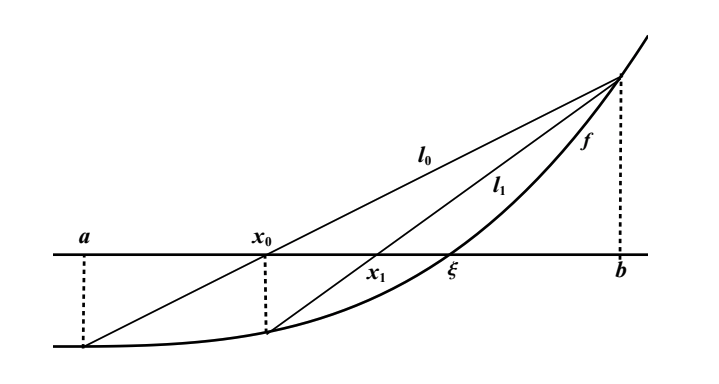
\includegraphics[width=0.8\linewidth]{fig_1.png}
  \caption{Геометрична илюстрация на метода на хордите.}
\end{figure}

\textbf{Формула за последователните приближения на метода на хордите}: Нека за определеност \(f''(x) > 0\), като на чертежа. Правата \(y = l_{n+1}(x)\) има уравнение: \[
  l_{n+1}(x) = f(x_n) + \frac{f(x) - f(b)}{x - b}(x-x_n)
\]  

Приближението \(x_{n+1}\) е корен на уравнението \(l_{n+1} = 0\)  и следователно: \[
x_{n+1} = x_{n} - \frac{f(x_n)}{f(x_{n}) - f(b)}(b - x_n)
\]  

\textbf{Сходимост на метода на хордите}: При направените предположения за \(f\) имаме, че \(f\) е изпъкнала, откъдето \(\{x_n\}\) е монотонна и ограничена редица, следователно е сходяща. Нека \(\underset{n \to \infty}{\lim}x_n = \alpha\). Тогава: \[
  \alpha = \alpha - \frac{f(\alpha)}{f(b) - f(\alpha)}(b - \alpha)
\]     

Получаваме, че \(f(\alpha) = 0\), следователно \(\alpha = \xi\), откъдето е доказана сходимостта на \(x_n\) към \(\xi\).

Сега ще разгледаме скоростта на сходимост. Ще докажем, че сходимостта на метода на хордите е със скоростта на геометричната прогресия. (Ще приложим следствието).

Имаме:\[
  \varphi(x) = x - \frac{f(x)}{f(b) - f(x)}(b-x)
\]  

Разглеждаме \(\varphi'(\xi)\):\[
  \varphi'(\xi) = 1 - \frac{f'(\xi)}{f(b) - f(\xi) }(\xi - b)
\]  

Но имаме, че \(f(\xi) = 0\), значи \[
  \varphi'(\xi) = 1 - \frac{f'(\xi)}{f(b)}(\xi - b) = \frac{f(b) - f'(\xi)(b - \xi)}{f(b)}
\]  

Като заместим \(f(b)\) по формулата на Тейлър имаме: \begin{align*}
  f(b) &= f(\xi) + f'(\xi)(b-\xi) + \frac{f''(\eta_1)}{2}(b-\xi)^{2} \text{ (в числителя) } \\
  f(b) &= f(\xi) +  f''(\eta_2)(b-\xi) \text{ (в знаменателя) }
\end{align*} 

\[
  \varphi'(\xi) = \frac{f''(\eta_1)(b-\xi)}{2f'(\eta_2)}
\] 

Нека \(M := \underset{t \in [a, b]}{\max}|f''(t)|\) и \(m := \underset{t \in [a, b]}{\min}|f'(t)|\). По условие имаме, че \(f'(t) > 0\) в \([a, b]\), следователно \(m > 0\). Оттук: \[
  |\varphi'(\xi)| \leq \frac{M}{2m}|b - \xi|
\]      

Ако \(b - \xi\) е достатъчно малко, то \(|\varphi'(\xi)|\) може да стане по-малко от произволно, предварително избрано \(q < 1\). Но \(b - \xi\) е достатъчно малко, стига интервалът \([a, b]\) да е достатъчно малък. И така ако \(\xi\) е в достатъчно малък интервал \([a, b]\), тo \(|\varphi'(\xi)| < q < 1\) и от следствието имаме, че итерационаият процес породен от \(\varphi\) е сходящ със скорост на геометричната прогресия.           

\subsection{Метод на секущите}

\textbf{Метод на секущите}: Нека \([a, b]\) е даден интервал и \(f(x)\) е два пъти диеференцируема в него функция, която удовлетворява условията: \begin{itemize}
    \item \(f(a)f(b) < 0\) 
    \item \(f'(x)f''(x) \not= 0, \forall x \in [a, b]\)  
\end{itemize}  

Означаваме \(M := \underset{t \in [a, b]}{\max}|f''(t)|\) и \(n := \underset{t \in [a, b]}{\min}|f'(t)|\)

Избираме \(x_0 = a\) или \(x_0 = b\), така че \(f(x_0)f''(x_0) > 0\) След това избираме точка \(x_1: \xi < x_1 < x_0\). Това става, когато \(x_0\) и \(x_1\) са от една и съща страна на \(\xi\), т.с.т.к. \(f(x_0)f(x_1) > 0\).

Построяваме \(x_{2}\) като пресечната точка на секущата \(l_1\) минаваща през точките \((x_0, f(x_0)), (x_1, f(x_1))\) и остта \(x.\)     

\begin{figure}[h!]
  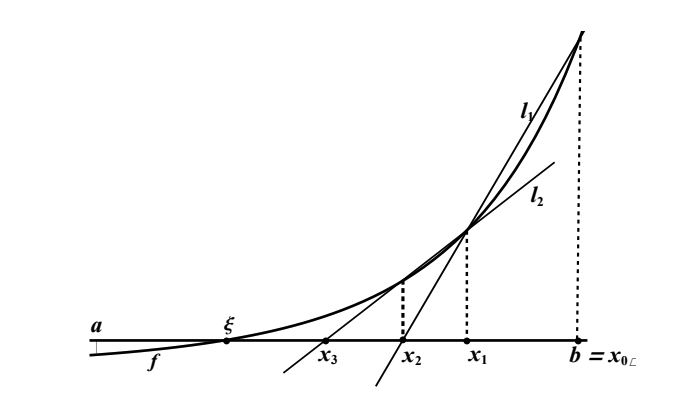
\includegraphics[width=0.8\linewidth]{fig_2.png}
  \caption{Геометрична илюстрация на метода на секущите.}
\end{figure}

\textbf{Формула за последователните приближения}: По формулата на Нютон имаме: \[
  l_n(x) = f(x_n) + \frac{f(x_n)}{f(x_{n-1}) - f(x_n)}(x-x_n)
\] 

\(x_{n+1}\) се определя от уравнението \(l_{n}(x) = 0\). Оттук формулата а пресмятане на \(x_{n+1}\) чрез \(x_n\) е: \[
  x_{n+1} = x_{n} - \frac{f(x_n)}{f(x_{n-1}) - f(x_n)}(x_{n-1} - x_n)
\]       

\textbf{Ред на сходимост}: \[
  |x_{n} - \xi| \leq Cq^{r^{n}}, \forall n
\] 

Тук \(r = \frac{1 + \sqrt{5}}{2}\)  

\subsection{Метод на Нютон}

\textbf{Метод на Нютон (на допирателните)}:  Нека \([a, b]\) е даден интервал и \(f(x)\) е два пъти диеференцируема в него функция, която удовлетворява условията: \begin{itemize}
    \item \(f(a)f(b) < 0\) 
    \item \(f'(x)f''(x) \not= 0, \forall x \in [a, b]\)  
\end{itemize}  

Означаваме \(M := \underset{t \in [a, b]}{\max}|f''(t)|\) и \(n := \underset{t \in [a, b]}{\min}|f'(t)|\)

Както при метода на секущите избираме приближение \(x_0 = 0\) или \(x_0 = b\), така че \(f(x_0)f''(x_0) > 0\).

Следващото приближение \(x_1\) се намира като пресечната точка на оста \(x\) с допирателната \(t_0\) към правата \(y = f(x)\) в точката \(x_0\).      

\begin{figure}[h!]
  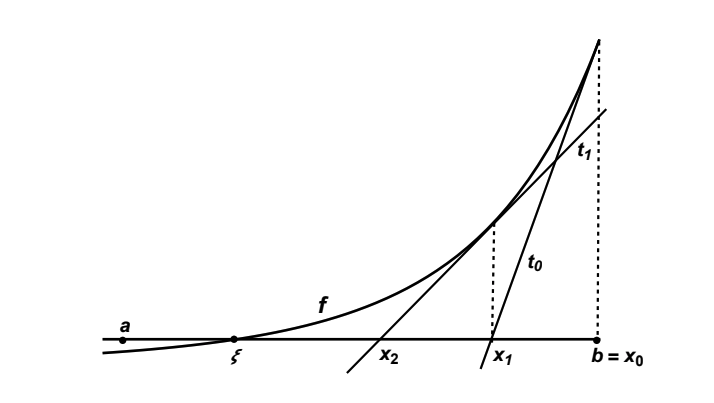
\includegraphics[width=0.8\linewidth]{fig_3.png}
  \caption{Геометрична илюстрация на метода на Нютон.}
\end{figure}

\textbf{Формула за последователните приближения}: Имаме, че \(x_{n+1}\) е нулата на допирателната \(t_n\) към \(f\) в точката \(x_n\). От условието \(l_{n}(x_{n+1}) = 0\), където: \[
  l_{n}(x) = f(x_n) - f'(x_n)(x-x_n)
\] 

намираме формулата за получаване на \(x_{n+1}\) от \(x_n\): \[
  x_{n+1} = x_n - \frac{f(x_n)}{f'(x_n)}
\]  

\textbf{Ред на сходимост}: \[
  |x_{n} - \xi| \leq Cq^{2^{n}},\qquad \forall n,\; q \in (0, 1)
\] 
\newpage
\section{Дискретни разпределения. Равномерно, биномно, геометрично и Поасоново разпределение. Задачи, в които възникват. Моменти - математическо очакване и дисперсия.}

\textbf{Ще се дадат две разпределения, които трябва да се опишат.}

\subsection{Дикстретно вероятностно разпределение на случайна величина}

\textbf{Сигма алгебра}: Нека \(\Omega\) е произволно множество и нека \(\mathcal{A} \in \mathcal{P(\Omega)}\). Казваме, че  \(\mathcal{A}\) е сигма алгебра, ако са изпълнени условията: \begin{itemize}
    \item \(\emptyset in \mathcal{A}\) 
    \item \(\Omega \in \mathcal{A}\) 
    \item Ако \(A \in \mathcal{A}\), то \(\bar{A} \in \mathcal{A}\) 
    \item Ако \(A_1, A_2,... \in \mathcal{A}\), то \(\bigcup_{i=1}A_i \in \mathcal{A}\) и \(\bigcap_{i=1}A_i \in \mathcal{A}\)    
\end{itemize}   

\textbf{Вероятност}: Вероятността \(P\) е функция, дефинирана върху сигма алгебрата \(\mathcal{A}\) от подмножества на \(\Omega\), която удовлетворява аксиомите:      

\begin{itemize}
    \item Неотрицателност: \(P(A) \geq 0\), за всяко събитие \(A \in \mathcal{A}\) 
    \item Нормираност: \(P(\Omega) = 1\) 
    \item Адитивност: Ако \(AB = \emptyset\), то \(P(A\cup B) = P(A) + P(B)\) 
    \item Непрекъснатост (монотонност): За всяка монотонно намаляваща редица \(A_1 \supset A_2 \supset ... \supset A_n \supset ...\), клоняща към празното множество е изпълнено \(\underset{n\to \infty}{\lim}P(A_n) = 0\)   
\end{itemize}

\textbf{Случайна величина}: Случайна величина наричаме функция \(X: \Omega \to \mathbb{R}\)  

\textbf{Дискретна случайна величина}: Нека \(\Omega = \underset{i}{\cup}H_{i}:\qquad H_{i} \cap H_{j} = \emptyset, i \not=j\), а \(x_i\) са произволни реални числа.  

Дискретна случайна величина наричаме: \[
  X(\omega) = \sum_{i}^{}x_iI_{H_i}(\omega)
\] 

Където \(I_{H_i}(\omega) = \begin{cases} 1, \omega \in H_{i} \\ 0, \omega \not\in H_{i}\end{cases}\) е индикатор на множеството \(H_{i}\) 

\textbf{Математическо очакване}: Нека \(X\) е дискретна случйна величина. Математическо очакване наричаме числото: \[
  \mathbb{E}X = \sum_{j}^{}x_jp_j, \text{ където }p_j = P(X=x_j)
\]  

\textbf{Дисперсия}: Нека \(X\) е произволна случайна величина. Дисперсия \(DX\) се дефинира с равенството:\[
  DX = \mathbb{E}(X - \mathbb{E}X)^{2}
\] 

Корен от дисперсията наричаме стандартно отклонение. 

\textbf{Пораждаща функция}: Нека \(X\) е случайна величина, чийто стойности са цели положителни числа. Пораждаща функция на \(X\) наричаме полином, в който пред \(k\)-тата степен на коефициента \(s\) стои вероятността \(P(X=k)\)    : \[
  g_{X}(s) = \sum_{k=0}^{\infty}P(X=k)s^{k}
\]   

\textbf{Свойства на пораждащата функция}:
\begin{itemize}
    \item \(\mathbb{E}X = g'_{X}(1)\) 
    \item \(DX = g''_{X}(1) + g'_{X}(1) - (g'_{X}(1))^{2}\)  
\end{itemize}

\subsection{Разпределение на Бернули}

\textbf{Разпределение на Бернули}: Нека \(X\) е случайна величина. \(X\) има разпредление на Бернули, ако прием две стойности: "1" при успех и "0" при неуспех. Може да се използва за хвърляне на монета - задаваме стойността "1" на ези, а "0" на тура.

Разпределението има вида: 

\begin{table}[]
\centering
  \begin{tabular}{lll}
  X    & 0 & 1     \\
  P & 1-p & p
  \end{tabular}
\end{table}  

\textbf{Математическо очакване}: \[
  \mathbb{E}X = 0(1-p) + 1.p = p
\] 

\[
  \mathbb{E}X^{2} = 0.(1-p)^{2} + 1.p^{2} = p^{2}
\] 

\textbf{Дисперсия}: \[
  DX = \mathbb{E}X^{2} - (\mathbb{E}X)^{2} = p - p^{2} = p(1-p)= pq
\] 

\subsection{Биномно разпределение}

\textbf{Биномно разпределение}: Извършват се \(n\) последователн, независими Бернулиеви опити, като вероятността за успех \(p\) на всеки опеит е една и съща. 

Случайната величина \(X\) равна на броят на успехите, наричаме биномно разпределена и записваме: \(X \in Bi(n, p)\). Вероятността за \(k\) успеха при n опита получаваме чрез: \[
  P(X=k) = \binom{n}{k}p^{k}(1-p)^{n-k}
\]  

Имаме: \begin{itemize}
    \item \(p^{k}\): Вероятността да имаме \(k\) успеха при \(n\) опита.
    \item \((1-p)^{n-k}\): Вероятността да имаме \(n-k\) неуспеха при \(n\) опита.
    \item \(\binom{n}{k}\): Броят различни подредби на успешните и неуспешните опити. 
  \end{itemize}

\underline{Коректност}: Формулата за бинома на Нютон ни дава: \[
  \sum_{k=1}^{n}P(X=k) = \sum_{k=1}^{n}\binom{n}{k}p^{k}(1-p)^{n-k} = (p+(1-p))^{n} = 1
\] 

\textbf{Пораждаща функция}:\[
  g_{X}(s) = \sum_{k=1}^{n}P(X=k)s^{k} = \sum_{k=1}^{n}\binom{n}{k}p^{k}(1-p)^{n-k}s^{k} = \sum_{k=1}^{n}\binom{n}{k}(ps)^{k}(1-p)^{n-k} = (ps + (1-p))^{n}
\]   

\textbf{Математическо очакване}: \[
  \mathbb{E}X = (n(ps + (1-p))^{n-1}p) \overset{s=1}{=} n(p + 1 - p)^{n-1}p = np
\] 

\textbf{Дисперсия}: 

\begin{align*}
  DX &= g''_{X}(1) + g'_{X}(1) - [g'_{X}(1)]^{2} = [n(n-1)(ps+(1-p))^{n-2}p^{2} + np - n^{2}p^{2}\\ 
     &= \overset{s=1}{=} n(n-1)(p+1-p)^{n-2}p^{2} + np - n^{2}p^{2} = \\ 
     &= n(n-1)p^{2} + np - (np)^{2} = np^{2} - np^{2} + np - (np)^{2} = np(1 - p) = npq
\end{align*}

Чрез биномното разпредлеение можем да пресметнем броя на шестиците при хвърляне на 4 зара.

\subsection{Геометрично разпределение}

Нека \(p\) е вероятността за успех, \(q = 1-p\) е вероятността за неуспех.  

\textbf{Геометрично разпределение}: Разглеждаме схема на Бернули с неограничен брой опити. Случайната величина \(X\) равна на "броя на неуспехите до достигане на първи успех" наричаме геометрично разпределена случайна величина и записваме \(X \in Ge(p)\). Вероятността да получим успех при \(k\)-тия опит получаваме пресмятайки: \[
  P(X=k) = (1-p)^{k}p
\] 

\underline{Коректност}: Прилагаме формулата за безкрайна геометрична прогресия: \[
  \sum_{k=0}^{\infty}P(X=k) = \sum_{k=}^{\infty}(1-p)^{k}p = \frac{p}{1-(1-p)}= 1
\] 

\textbf{Пораждаща функция}:\[
  g_{X}(s) = \sum_{k=0}^{\infty}P(X=k)s^{k} = \sum_{k=0}^{\infty}q^{k}ps^{k} = p \sum_{k=0}^{\infty}(qs)^{k} = \frac{p}{1 - qs}
\] 

\textbf{Математическо очакване}: \[
  \mathbb{E}X = g'_{X}(1) = p \left(\frac{q}{(1-qs)^{2}}\right) \overset{s=1}{=} \frac{pq}{(1-q)^{2}} = \frac{pq}{p^{2}} = \frac{p}{q}
\] 

\textbf{Дисперсия}:
\[
  g''_{X}(1) = \left(\frac{pq}{(1-qs)^{2}}\right)^{\prime} \overset{s=1}{=} \frac{2pq^{2}}{(1-q)^{3}} = \frac{2pq^{2}}{p^{3}} = \frac{2q^{2}}{p^{2}}
\]  
\[
  DX = g''_{X}(1) + g'_{X}(1) - (g'_{X}(1))^{2} = \frac{2q^{2}}{p^{2}} + \frac{q}{p} - \frac{q^{2}}{p^{2}} = \frac{q(q+p)}{p^{2}} = \frac{q}{p^{2}}
\] 

Чрез отрицателното разпределение можем да пресметнем броя хвърляния на зар, докато не се падне шестица.

\subsection{Отрицателно биномно разпределение}

\textbf{Отрицателно биномно разпределение}: Разглеждаме схема на Бернули с неограничен брой опити. Случайната величина \(X\) равна на "броя на неуспехите до достигане на r-тия успех" наричаме отрицателно биномно разпределена и записваме \(X \in NB(r, p)\). За да пресметнем вероятността да сме получили \(r\) успеха след \(k\) опита пресмятаме: \[
  P(X=k) = \binom{r+k-1}{k}p^{r}q^{k} = \binom{r+k-1}{r-1}p^{r}q^{k}
\]   

Имаме: \begin{itemize}
  \item \(\binom{r+k-1}{r-1}\): Броят различни начини, по който може да сме получили \(k\) неуспеха и \(r-1\) успеха.
  \item \(p^{r-1}q^{k}\): Вероятността да сме получили \(k\) неуспеха и \(r-1\) успеха.
  \item Умножаваме всичко по \(p\) - вероятността \(r\)-тия (последния) опит да е успех.  
\end{itemize}

\textbf{Коректност}: \[
  \sum_{k=0}^{\infty}P(X=k) = p^{r}\sum_{k=0}^{\infty}\binom{r+k-1}{r-1}q^{k} = \frac{p^{r}}{(1-q)^{r}} = 1
\] 

За да пресметнем очакването и дисперсията ще въведем случайните величини: \begin{itemize}
    \item \(X_1\) броят на неуспехите до първия успех.
    \item \(X_2\) броят на неуспехите между първия и втория успех.
    \item ...
    \item \(X_{r}\) броят на неуспехите между \(r-1\)-вия и \(r\)-тия успех.   
\end{itemize}


Тъй като опитите са независими, то и случайните величини са независими. Имаме, че \(X_{i} \in Ge(p)\).

Имаме, че \(X = X_1 + ...+X_r\), откъдето можем да разгледаме отрицателното биномно разпределение като сума от геометрични разпределения. 

Знаем, че пораждащата функция на \(X_i\) е: \[
  g_{X_i}(s) = \frac{p}{1- qs}
\] 

За пораждащата функция на \(X\) получаваме: \[
  g_{X}(s) = g_{X_1+...X_r}(s) = \prod_{i=1}^{r}g_{X_i}(S)=\frac{p^{r}}{(1-qs)^{r}}
\]  

Прилгаме формулата за отрицателен бином и имаме: \[
  \frac{p^{r}}{(1-qs)^{r}} = p^{r}\sum_{k=0}^{\infty}\binom{r+k-1}{k}q^{k}s^{k} = \sum_{k=0}^{\infty}P(X=k)s^{k}
\] 

Виждаме, че \(X \in NB(r,p)\). От свойствата на очакването и дисперсията имаме: 

\textbf{Математическо очакване}: \[
  \mathbb{E}X = \mathbb{E}(X_1 + ... + X_r) = r \mathbb{E}X_1 = r \frac{p}{q}
\] 

\textbf{Дисперсия}: \[
  DX = r \frac{q}{p^{2}}
\]   

С отрицателното биномно разпределение можем да пресметнем броя хвърляния на монета, докато не сме хвърлили 10 езита.

\subsection{Поасоново разпределение}

\textbf{Поасоново разпределение}: Поасоновото разпределение се използва, когато имаме голям брой събития с малка вероятност за успех, частен случай на биномното при \(n \to \infty, p \to 0\). Казваме, че случайната величина \(X\) равна на броя на успехите е поасоново разпределена и пишем \(X \in Po(\lambda)\). Пресмятаме вероятността за \(k\) успеха чрез:\[
  P(X=k) = \frac{\lambda^{k}e^{-\lambda}}{k!}
\] 

Тук \(\lambda > 0\) е константа. 

\textbf{Коректност}: \[
  \sum_{k=0}^{\infty}\frac{\lambda^{k}e^{-\lambda}}{k!} = e^{-\lambda}\sum_{\lambda^{k}}^{k!} = e^{-\lambda}e^{\lambda} = 1
\] 

\textbf{Пораждаща функция}: 
\[
  g_{X}(s) = \sum_{k=0}^{\infty}P(X=k)s^{k} = \sum_{k=0}^{\infty}\frac{\lambda^{k}e^{-\lambda}}{k!}s^{k} = e^{-\lambda}\sum_{(s\lambda)^{k}}^{k!} = e^{-\lambda}e^{s\lambda} = e^{\lambda(s-1)}
\] 

\textbf{Математическо очакване}: \[
  \mathbb{E}X = g'_{X}(1) = \lambda e^{\lambda(s-1)} \overset{s=1}{=}\lambda
\] 

\textbf{Дисперисия}: 
\[
  DX = g''_{X}(1) + g'_{X}(1) - [g'_{X}(1)]^{2} = \lambda^{2}e^{\lambda(s-1)} + \lambda - \lambda^{2} \overset{s=1}{=} \lambda^{2} + \lambda - \lambda^{2} = \lambda 
\] 

Пример: Произвеждаме 1000 детайла на ден. Вероятността един детайл да е дефектен е \(1/1000\). Получаваме \(\lambda = np = 1\). Вероятността два детайла да се дефектни е: \[
  P(X=2) = \frac{\lambda^{2}e^{-\lambda}}{2!} = \frac{1e^{-1}}{2} = \frac{1}{2e}
\]    
\end{document}

